%\documentclass[a4paper,12pt,twoside]{book}
\documentclass[12pt,times]{report}
\usepackage{mathptmx}%This package supersedes times and mathptm
\usepackage[a4paper,right=2.54cm,left=2.54cm,top=2.54cm,bottom=2.54cm]{geometry}

%%%%paquete para usar citas de diferentes formatos
%%%%%%%%%%%%%%%%%%%%%%%%%%%%%%%%%
%%add al indice
%\usepackage[nottoc,numbib]{tocbibind}
%\usepackage[authoryear,round]{natbib}
\usepackage[utf8]{inputenc}
\usepackage{csquotes}
\usepackage[spanish]{babel}
\usepackage[style=apa ,
%hyperref=auto,
%citestyle=authoryear,
natbib=true,
backend=biber]{biblatex}
\addbibresource{biblio/references.bib}
%\usepackage{biblatex}
%paquete para hiperlinks entre citas e imagenes
%%%%%%%%%%%%%%%%%%%%%%%%%%%%%%%%%
\usepackage[colorlinks=true,
citecolor=blue,
urlcolor=cyan,
bookmarks=true,
linkcolor=blue,
pdftitle={Tesis-nombre-alumno},
pdfauthor={autor nombres}]{hyperref}

\usepackage{amssymb}
\usepackage{graphicx} % for improved inclusion of graphics
%\usepackage{wrapfig} % to include figure with text wrapping around it
\usepackage[margin=10pt,font=small,labelfont=bf]{caption} % for improved layout of figure captions with extra margin, smaller font than text
\usepackage{eucal}
\usepackage[usenames, dvipsnames]{color}
\usepackage[perpage]{footmisc}
%\usepackage[round, sort]{natbib}
\usepackage{ifthen}
\usepackage{multicol} % for pages with multiple text columns, e.g. References
\setlength{\columnsep}{20pt} % space between columns; default 10pt quite narrow
\usepackage[nottoc]{tocbibind} % correct page numbers for bib in TOC, nottoc suppresses an entry for TOC itself
\usepackage{appendix}

%%%----Modificar encabezado y pie de pagina
%%%%%%%%%%%%%%%%%%%%%%%%%%%%%%%%%%%%%%%%%%%%%%%%%%%%%%%%%%%%%%%%%%%%%
\usepackage{fancyhdr} % for better header layout
\newcommand{\changefont}{%
	\fontsize{9pt}{1.5pt}\selectfont
}
\pagestyle{fancy}
\fancyhf{} %% delete default configuration of page
%%\setlength\headheight{15pt}
\fancyhead[L]{\changefont Titulo de tesis aqui}
\fancyhead[R]{\changefont \leftmark}
%%\fancyfoot[L]{\leftmark}
\fancyfoot[R]{\thepage}

%%%%%%%%%%%%%%%%%%%%%%%%%%%%%5
%%%% Configuracion de los parrafos
%\usepackage{setspace}
%\onehalfspacing
%\linespread{1.25} 
\setlength{\parindent}{0.5in} %%sangria
\setlength{\parskip}{3mm}  %%espacio entre parrafos
\linespread{1.3} %This equals 1.5 linespacing in Word
%%%% nuevo parrafo
%%%%%%%%%%%%%%%%%%%%%%%%%%%%%5
%%%% Centrar valores de una tabla
\usepackage{array}
%%CENTRADO HORIZONTAL
\newcolumntype{P}[1]{>{\centering\arraybackslash}p{#1}}
%%CENTRADO VERTICAL
\newcolumntype{M}[1]{>{\centering\arraybackslash}m{#1}}

%%%%%%%%%%%%%%%%%%%%%%%%%%%%%5
%%%%Paquete para alinear texto
\usepackage{ragged2e}
\usepackage{multirow}
\usepackage{makecell}
\usepackage{rotating}
\usepackage{siunitx} % To align the numbers later on
\usepackage[table,xcdraw]{xcolor}
\usepackage{color, colortbl}
\definecolor{Gray}{gray}{0.9}
\definecolor{orange}{rgb}{1,0.647,0}
\definecolor{turq3}{rgb}{0.54, 0.81, 0.94}
\definecolor{turq}{rgb}{0.63, 0.79, 0.95}
\definecolor{bluejean}{rgb}{0.03, 0.27, 0.49}

%%%%%%%%%%%%%%%%%%%%%%%%%
\usepackage{xparse}
\usepackage{expl3}
%%%%funcion de reemplazar regex
\ExplSyntaxOn
\NewDocumentCommand{\replace}{mmm}
{
	\marian_replace:nnn {#1} {#2} {#3}
}

\tl_new:N \l_marian_input_text_tl
\tl_new:N \l_marian_search_tl
\tl_new:N \l_marian_replace_tl

\cs_new_protected:Npn \marian_replace:nnn #1 #2 #3
{
	\tl_set:Nn \l_marian_input_text_tl { #1 }
	\tl_set:Nn \l_marian_search_tl { #2 }
	\tl_set:Nn \l_marian_replace_tl { #3 }
	\regex_replace_all:nnN { \b\u{l_marian_search_tl}\b } { \u{l_marian_replace_tl} } \l_marian_input_text_tl
	\tl_use:N \l_marian_input_text_tl
}
\ExplSyntaxOff

%%%%%%%%%%%%%%%%%%%%%%%%%%%%%%%%%%%%%%
\usepackage{amsmath}
\numberwithin{equation}{chapter} %%enumerar ecuaciones
\renewcommand{\theequation}{Ecuación \thechapter.\arabic{equation}}   
\usepackage{mathtools, nccmath, cool}
%%%Configuraciones de biblatex

%%%hel
%%%%\citeauthor
\makeatletter

%%%%%%%%%%%%
\DeclareCiteCommand{\citeauthor}
{\boolfalse{citetracker}%
	\boolfalse{pagetracker}%
	\usebibmacro{prenote}}
{\ifciteindex
	{\indexnames{labelname}}
	{}%
	\printtext[bibhyperref]{\printnames{labelname}}}
{\multicitedelim}
{\usebibmacro{postnote}}


\DeclareCiteCommand{\citetitle}
{\boolfalse{citetracker}%
	\boolfalse{pagetracker}%
	\usebibmacro{prenote}}
{\ifciteindex
	{\indexfield{indextitle}}
	{}%
	\printtext[bibhyperref]{\printfield[citetitle]{labeltitle}}}
{\multicitedelim}
{\usebibmacro{postnote}}

\DeclareCiteCommand{\cite}
{\usebibmacro{prenote}}
{\usebibmacro{citeindex}%
	\printtext[bibhyperref]{\usebibmacro{cite}}}
{\multicitedelim}
{\usebibmacro{postnote}}

\DeclareCiteCommand*{\cite}
{\usebibmacro{prenote}}
{\usebibmacro{citeindex}%
	\printtext[bibhyperref]{\usebibmacro{citeyear}}}
{\multicitedelim}
{\usebibmacro{postnote}}

\DeclareCiteCommand{\parencite}[\mkbibparens]
{\usebibmacro{prenote}}
{\usebibmacro{citeindex}%
	\printtext[bibhyperref]{\usebibmacro{cite}}}
{\multicitedelim}
{\usebibmacro{postnote}}

\DeclareCiteCommand*{\parencite}[\mkbibparens]
{\usebibmacro{prenote}}
{\usebibmacro{citeindex}%
	\printtext[bibhyperref]{\usebibmacro{citeyear}}}
{\multicitedelim}
{\usebibmacro{postnote}}

\DeclareCiteCommand{\footcite}[\mkbibfootnote]
{\usebibmacro{prenote}}
{\usebibmacro{citeindex}%
	\printtext[bibhyperref]{ \usebibmacro{cite}}}
{\multicitedelim}
{\usebibmacro{postnote}}

\DeclareCiteCommand{\footcitetext}[\mkbibfootnotetext]
{\usebibmacro{prenote}}
{\usebibmacro{citeindex}%
	\printtext[bibhyperref]{\usebibmacro{cite}}}
{\multicitedelim}
{\usebibmacro{postnote}}

\DeclareCiteCommand{\textcite}
{\boolfalse{cbx:parens}}
{\usebibmacro{citeindex}%
	\printtext[bibhyperref]{\usebibmacro{textcite}}}
{\ifbool{cbx:parens}
	{\bibcloseparen\global\boolfalse{cbx:parens}}
	{}%
	\multicitedelim}
{\usebibmacro{textcite:postnote}}
\makeatother
\makeatletter
\let\abx@macro@citeOrig\abx@macro@cite
\renewbibmacro{cite}{%
	\bibhyperref{%
		\let\bibhyperref\relax\relax%
		\abx@macro@citeOrig%
	}%
}
\let\abx@macro@textciteOrig\abx@macro@textcite
\renewbibmacro{textcite}{%
	\bibhyperref{%
		\let\bibhyperref\relax\relax%
		\abx@macro@textciteOrig%
	}%
}%

\makeatother

%%%%%%%%%%%%%%%%%%%%%%%%%%%%%%%%%%%%%%%%%%%
\begin{document}

\begin{titlepage}

	\begin{center}
		%%%cargar imagen
	    
\includegraphics[width=0.45\textwidth]{images_repo/esanlogomin}
		\vspace*{2cm} \\
		UNIVERSIDAD ESAN \vspace*{1ex} \\
		FACULTAD DE INGENIERÍA \vspace*{1ex} \\
		INGENIERÍA DE TECNOLOGÍAS DE INFORMACIÓN Y SISTEMAS\vspace*{8ex} \\
		\textbf{Aplicación de técnicas de Visión Computacional para la clasificación temprana de "Rancha" Phytophthora infestans en las hojas de papa peruano}
		\vspace*{8ex}\\	
		Trabajo de investigación para el curso de Trabajo de Tesis I 
		\vspace*{8ex} \\	
		Sebastian Puruguay \\
		Asesor: Marks Calderón		
		\vfill
		
		Lima, \today 
		
	\end{center}
\end{titlepage}
%%cambiar nombres de objetos para el indice y otros
\renewcommand{\listfigurename}{Índice de Figuras}
\renewcommand{\tablename}{Tabla}
\renewcommand{\listtablename}{Índice de Tablas}

%% Agregar al terminar
%%%La línea de abajo es para quitar encabezado
%\thispagestyle{plain}

\chapter*{Resumen}
\markboth{Resumen}{Resumen}
\addcontentsline{toc}{chapter}{Resumen}


%\newline

\textbf{Palabras claves: } 

\clearpage
%\vspace{0.5cm}
\chapter*{Abstract}
\markboth{Abstract}{Abstract}

%\newline

\textbf{Keywords: } 
%%\thispagestyle{plain}
\begin{center}
	\vspace*{1.5cm}
	{\Large \bfseries  Abstract}
\end{center}
\vspace{0.5cm}
Lorem ipsum dolor sit amet, consectetur adipiscing elit, sed do eiusmod tempor incididunt ut labore et dolore magna aliqua. Ac odio tempor orci dapibus ultrices in iaculis nunc sed. Vivamus arcu felis bibendum ut tristique et egestas quis ipsum. Odio morbi quis commodo odio aenean sed adipiscing diam donec. Donec ultrices tincidunt arcu non sodales neque sodales ut. Fusce ut placerat orci nulla pellentesque dignissim enim sit amet. Facilisi etiam dignissim diam quis enim lobortis. Sit amet justo donec enim diam vulputate ut pharetra. Gravida in fermentum et sollicitudin ac orci phasellus egestas. Ultricies tristique nulla aliquet enim tortor at auctor. Nullam vehicula ipsum a arcu cursus vitae congue mauris. Convallis posuere morbi leo urna molestie at elementum eu facilisis. Elit at imperdiet dui accumsan sit amet nulla. Amet consectetur adipiscing elit pellentesque habitant morbi tristique senectus et. Mauris in aliquam sem fringilla ut morbi. Ultricies integer quis auctor elit sed vulputate mi sit. Nulla pellentesque dignissim enim sit amet venenatis urna cursus eget. Ac feugiat sed lectus vestibulum mattis ullamcorper. Eu augue ut lectus arcu bibendum. Rhoncus dolor purus non enim praesent elementum. 

Nulla facilisi cras fermentum odio eu feugiat pretium. Massa massa ultricies mi quis hendrerit. Id leo in vitae turpis massa sed elementum. Quis vel eros donec ac odio tempor orci. Netus et malesuada fames ac turpis egestas integer eget aliquet. Velit ut tortor pretium viverra suspendisse potenti. Ut enim blandit volutpat maecenas. Nibh tellus molestie nunc non blandit. Mus mauris vitae ultricies leo integer malesuada nunc vel. Vel elit scelerisque mauris pellentesque pulvinar pellentesque habitant. Neque viverra justo nec ultrices dui sapien eget. Vitae aliquet nec ullamcorper sit. Dui id ornare arcu odio ut sem nulla pharetra diam. Et magnis dis parturient montes. Varius morbi enim nunc faucibus.
\newline

\textbf{Keywords: } uno, dos, tres, cuatro
%%\thispagestyle{plain}
\begin{center}
	\vspace*{1.5cm}
	{\Large Para mi X, Y,X}
\end{center}


%%\thispagestyle{plain}
\begin{center}
	\vspace*{1.5cm}
	{\Large \bfseries  Agradecimientos}
\end{center}
\vspace{0.5cm}
Lorem ipsum dolor sit amet, consectetur adipiscing elit, sed do eiusmod tempor incididunt ut labore et dolore magna aliqua. Ac odio tempor orci dapibus ultrices in iaculis nunc sed. Vivamus arcu felis bibendum ut tristique et egestas quis ipsum. Odio morbi quis commodo odio aenean sed adipiscing diam donec. Donec ultrices tincidunt arcu non sodales neque sodales ut. Fusce ut placerat orci nulla pellentesque dignissim enim sit amet. Facilisi etiam dignissim diam quis enim lobortis. Sit amet justo donec enim diam vulputate ut pharetra. Gravida in fermentum et sollicitudin ac orci phasellus egestas. Ultricies tristique nulla aliquet enim tortor at auctor. Nullam vehicula ipsum a arcu cursus vitae congue mauris. Convallis posuere morbi leo urna molestie at elementum eu facilisis. Elit at imperdiet dui accumsan sit amet nulla. Amet consectetur adipiscing elit pellentesque habitant morbi tristique senectus et. Mauris in aliquam sem fringilla ut morbi. Ultricies integer quis auctor elit sed vulputate mi sit. Nulla pellentesque dignissim enim sit amet venenatis urna cursus eget. Ac feugiat sed lectus vestibulum mattis ullamcorper. Eu augue ut lectus arcu bibendum. Rhoncus dolor purus non enim praesent elementum. 

Nulla facilisi cras fermentum odio eu feugiat pretium. Massa massa ultricies mi quis hendrerit. Id leo in vitae turpis massa sed elementum. Quis vel eros donec ac odio tempor orci. Netus et malesuada fames ac turpis egestas integer eget aliquet. Velit ut tortor pretium viverra suspendisse potenti. Ut enim blandit volutpat maecenas. Nibh tellus molestie nunc non blandit. Mus mauris vitae ultricies leo integer malesuada nunc vel. Vel elit scelerisque mauris pellentesque pulvinar pellentesque habitant. Neque viverra justo nec ultrices dui sapien eget. Vitae aliquet nec ullamcorper sit. Dui id ornare arcu odio ut sem nulla pharetra diam. Et magnis dis parturient montes. Varius morbi enim nunc faucibus.
\newline



% outline
\tableofcontents            % print the table of contents

%: ----------------------- contents ------------------------

\setcounter{secnumdepth}{3} % organisational level that receives a numbers
\setcounter{tocdepth}{3}    % print table of contents for level 3

% levels are: 0 - chapter, 1 - section, 2 - subsection, 3 - subsection


%: ----------------------- list of figures/tables ------------------------

%%\listoffigures	% print list of figures

%%\listoftables  % print list of tables



\chapter{PLANTEAMIENTO DEL PROBLEMA}
\section{Descripción de la Realidad Problemática}


Hoy en día, la producción de papa es una de las actividades más importantes en nuestro país tanto a nivel económico como alimenticio y el Perú es el mayor productor de papa en América Latina contando con más de 4mil variedades.\parencite{cr_elcomercioproduccionpapa}.  


De acuerdo al reporte del Ministerio de Desarrollo Agrario y Riego (Midagri) del 2023, el consumo de papa por persona es de, aproximadamente, 92 kilos por año, cifra que ha venido incrementándose desde hace dos décadas debido a la importancia que tiene este tubérculo en la dieta de los peruanos. La papa es considerada uno de los alimentos más importantes y nutritivos en el Perú, rico en carbohidratos, proteínas, vitaminas y minerales.  Mientras que otros productos relevantes como el arroz no se cultivan en más de 7 regiones, lo que evidencia la amplia distribución geográfica del cultivo de papa en el territorio peruano \parencite{cr_agroinforma1}. Asimismo, el tubérculo se siembra en 19 distintas regiones del país, resaltando en departamentos como Puno y Huánuco, que lideran la producción nacional con 20.6\% y 12.6\% respectivamente \parencite{minagri_estadisticas_2022}. También, según el Censo Nacional Agropecuario 2022, el cultivo de papa es el sustento de al menos 710,000 familias en el Perú, representando aproximadamente el 25\% de los hogares dedicados a la agricultura y aportando el 6.5\% al PBI agropecuario del país \parencite{inei_cenagro_2022}.

Sin embargo, el los últimos años, la producción se ha visto afectada por una de las patologías más mortales que es Phytophthora infestans, conocido por los agricultores como Rancha o tizón tardío, la cual es capaz de acabar con el 100\% de cultivos enteros en solo unos días sino se antepone una medida de prevención. Según el técnico del Servicio para el Desarrollo Integral Rural,   la rancha es peligrosa y puede arruinar  toda la siembra. Es relevante para el agricultor diagnosticarla y encontrar la mejor manera de controlarla. Las condiciones climáticas propicias para la aparición de la rancha o tizón tardío se dan cuando las temperaturas fluctúan entre los 15°C y 18°C, o bien, cuando la temperatura se mantiene por debajo de los 25°C durante un periodo de 7 días consecutivos. Asimismo, esta enfermedad se ve favorecida por la presencia de lluvias constantes o cuando los niveles de humedad relativa oscilan entre el 90\% y el 100\% \cite{cr_rancha1}. Los principales síntomas de la enfermedad en el tubérculo son: hojas, lesiones en los bordes mostrando manchas necróticas con halo amarillento y micelio blanquecino en el relieve de la hojas; tallos, lesiones que recorren el tallo de color marrón osucro; tubérculos, lesiones irregulares en de color marrón rojizo que no solo están presentes en los alrededores de la papa sino del al interior también \parencite{cr_rancha2}. 

\begin{figure}[h]
	\begin{center}
		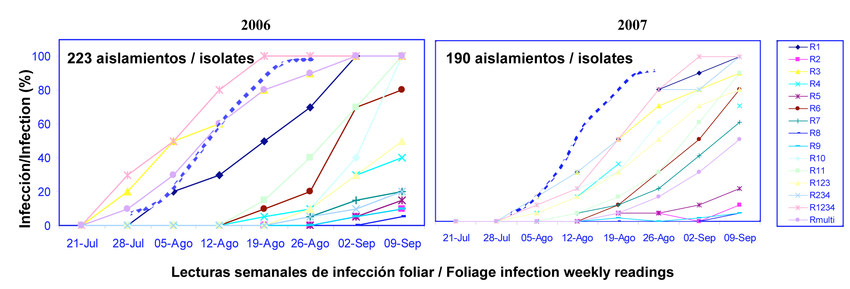
\includegraphics[width=1\textwidth]{1/figures/evolucionrancha.png}
		\caption[Lecturas semanales de infección foliar]{Lecturas semanales de infección foliar\\
			Fuente: \cite{cr_gestion2018emprend}. \textit{El tizón tardío es capaz de llegar a un alto porcentaje de severidad en solo dos semanas}.}
		\label{1:fig}
	\end{center}
\end{figure}

El caso más popular sobre rancha en Perú ocurrió en 2010 afectando a la región de Junín, donde al menos 26 mil de toneladas de papa fueron afectadas por la rancha en dos mil 660 hectáreas , lo cual representó una pérdida de 10 millones de nuevos soles. Esto se pudo evitar con fungicidas; sin embargo, estos son costosos entonces no todos los agricultores tiene accesso a este \parencite{cr_rancha6}. 

En abril de 2024, la rancha afectó a sembríos de papa nativa en la sierra de Lima, según resportes el tizón tardío arrasó con tres custodios de papa autóctonos tres en Huarachorí, dos en Yauyos y uno en Cajatambo \parencite{cr_rancha3}. Asimismo, en marzo de 2024, la rancha afectó fuertemente en el departamento de Junín, haciendo que 2000 agricultores pierdan, aproximadamente, 550 héctareas de papa por el tizón tardío, valorizando esta pérdida en S/300 mil. Siendo este el principal cultivo agricola en su sierra \parencite{cr_rancha4}. Finalmente, en abril de 2024, la rancha atacó el departamento de Apúrimac, la cual perdió una hectárea de papa y una y media hectáreas de cultivos afectados \parencite{cr_rancha5}.

Ante esto, el gobierno se ha visto obligado a concientizar sobre la rancha, en marzo de 2024, el Servicio para el Desarrollo Integral Rural (Sedir) y Servicio Nacional de Sanidad Agraria (Senasa) en Ancash, ya que varios agricultores locales temen perder sus sembríos debido a la rancha, principalmente porque se desarolla en temperaturas entre 12°C y 16°C y con fuerte presencia de humedad. Según la charla, una forma de prevenir la rancha es rotando el cultivo, es decir cambiando a otros productos como maíz y alverja \parencite{cr_agroinforma2}.

Por eso mismo, con el gran avance de la Inteligencia Artificial (IA) se ha perfeccionado y popularizado su uso en el sector agrícola de distintas formas, ya que es una herramienta útil y apta para procesar enormes cantidades de información rápidamente. . La IA es una alternativa tecnología que puede brindar soluciones prácticas porque es eficiente creando algoritmos capaces de detectar patologías a tiempo, así como mejorar tanto la precisión del diagnóstico como la eficiencia del flujo de trabajo en el campo, además que reduce costes porque agiliza. La IA también se puede emplear para identificar a plantas que están en peligro de pescar una enfermedad específica, lo que facilita la intervención y prevención temprana. Por ejemplo, un estudio reciente mostró que un sistema de IA logró detectar la zona enferma de una hoja con una precision deñ 96.44\% \parencite{cr_iaplanta}.

Añadiendo, la adopción de tecnología de IA en el ámbito de la agricultura del Perú puede ofrecer soluciones para una serie de problemas que enfrenta el sistema de siembra y cosecha, como el bajo acceso a asistencia técnica  en este sector en el país, la escasez de personal, la falta de competencias y la insuficiencia de equipos tecnológicos para una mejor desempeño para el proceso agrícola. En muchas ocasiones, particularmente en las zonas rurales y de recursos limitados, la falta de tecnología agrícola adecuada puede restringir la productividad y la calidad de los cultivos en la agricultura peruana. Sin embargo, al emplear herramientas de inteligencia artificial, como sistemas de monitoreo automatizado de cultivos y análisis de datos agrícolas, se puede incrementar la eficiencia en la producción, reducir los costos y garantizar una mayor calidad de los productos agrícolas, beneficiando así a más agricultores y contribuyendo al desarrollo sostenible del sector.En muchos casos, especialmente en las áreas rurales y de bajos ingresos del Perú, la falta de equipamiento agrícola básico y adecuado limita el rendimiento y la productividad de los cultivos. Al utilizar herramientas de inteligencia artificial, como sistemas de monitoreo de cultivos, análisis de patologías en cultivos y predicción del clima, se puede mejorar la toma de decisiones en cuanto a la siembra, el riego y la aplicación de insumos, optimizando los recursos y aumentando los rendimientos, lo que permite una mayor producción agrícola para alimentar a más personas. Un porcentaje significativo de los trabajos se enfocan en la detección y diagnóstico de enfermedades (29.4\%) y en la recomendación de fertilizantes (29.4\%), sin embargo, este último aspecto no abarca específicamente el cultivo de maíz. Los sistemas expertos están diseñados principalmente para que el agricultor pueda tomar decisiones más acertadas durante el ciclo de cultivo, lo cual representa el 80.6\% de los casos. Estos sistemas se consideran usuarios potenciales, ya que muchos agricultores no tienen los recursos para contratar a un experto en el área. Los sistemas expertos ofrecen una alternativa accesible y de bajo costo \parencite{cr_iaplanta2}. 


En este sentido, la presente investigación busca desarrollar e implementar un sistema robusto y escalable de visión computacional, aprovechando los avances tecnológicos más recientes, con el fin de proporcionar una solución innovadora, accesible y de alto impacto para los agricultores peruanos, facilitando la lucha contra esta devastadora enfermedad y promoviendo la resiliencia y productividad de los cultivos de papa a nivel nacional.

\section{Formulación del Problema}
Para formular los problemas de esta investigación, se creó un "árbol de problemas". (véase Anexo \ref{anexos:arbol_problema}).
\subsection{Problema General}
\newcommand{\ProblemaGeneral}{
	¿Es posible desarrollar un sistema de visión computacional que permita la clasificación temprana de la rancha (Phytophthora infestans) en hojas de papa peruana con alta precisión?
}
\ProblemaGeneral
\subsection{Problemas Espec\'{i}ficos}
\newcommand{\Pbone}{
	¿Cómo podemos desarrollar un sistema de detección automática de Rancha Phytophthora infestans en las hojas de papa peruana que sea preciso, eficiente y robusto a la variabilidad de las lesiones y las condiciones ambientales?
}
\newcommand{\Pbtwo}{
	¿Cómo obtener un conjunto de datos representativo y diverso de imágenes de hojas de papa con Rancha y sin ella?
}
\newcommand{\Pbthree}{
	¿Cuáles son las técnicas de visión computacional más apropiadas para la detección temprana de Rancha en hojas de papa peruano?
}
\newcommand{\Pbfour}{
	¿Cuáles son las técnicas de preprocesamiento de imágenes más apropiadas para la detección temprana de Rancha en hojas de papa peruano??
}

\begin{itemize}
	\item \Pbone
	\item \Pbtwo
	\item \Pbthree
	\item \Pbfour
\end{itemize}

\section{Objetivos de la Investigación} 
\subsection{Objetivo General}
\newcommand{\ObjetivoGeneral}{
	Desarrollar un sistema de visión computacional basado en técnicas de aprendizaje profundo para la clasificación temprana de la rancha (Phytophthora infestans) en hojas de papa peruana.
}
\ObjetivoGeneral
\subsection{Objetivos Espec\'{i}ficos}
\newcommand{\Objone}{
	Desarrollar un sistema de detección automática de Rancha Phytophthora infestans que alcance una precisión alta en la detección de lesiones en las hojas de papa.
}
\newcommand{\Objtwo}{
	Recolectar un conjunto de datos amplio y diverso de imágenes de hojas de papa que cubra una variedad de condiciones y escenarios relevantes para la detección de la Rancha.
}
\newcommand{\Objthree}{
	Identificar las técnicas de visión computacional más adecuadas para la detección temprana de Rancha en hojas de papa peruana.
}
\newcommand{\Objfour}{
	Identificar las técnicas de preprocesamiento de imágenes más adecuadas para la detección temprana de Rancha en hojas de papa peruana.
}

\begin{itemize}
	\item {\Objone}
	\item {\Objtwo}
	\item {\Objthree}
	\item {\Objfour}
\end{itemize}

\section{Hipótesis}

\subsection{Hipótesis General}
\newcommand{\HipotesisGeneral}{
	Se sostiene que mediante el desarrollo de un sistema de clasificación automática de las lesiones de Rancha Phytophthora infestans en las hojas de papa peruana, se puede lograr un método de detección la Rancha en las hojsa de papa peruana.
}
\HipotesisGeneral
\subsection{Hipótesis Específicas}
\newcommand{\Hone}{
	La implementación de técnicas de aprendizaje automático y detección de imágenes permitirá desarrollar un sistema de detección automática de Rancha Phytophthora infestans con alta precisión.
}
\newcommand{\Htwo}{
	La recopilación de un conjunto de datos representativo y diverso proporcionará una base sólida para el entrenamiento y la validación de los algoritmos de visión computacional, lo que mejorará su capacidad para detectar con precisión la Rancha en las hojas de papa.
}
\newcommand{\Hthree}{
	Se sostiene que al investigar específicamente técnicas de visión computacional, se logrará una mejora significativa en la detección temprana de Rancha en hojas de papa peruano.
}
\newcommand{\Hfour}{
	Se sostiene que al investigar específicamente técnicas de preprocesamiento de imágenes, se logrará una mejora significativa en la detección temprana de Rancha en hojas de papa peruano.
}
\begin{itemize}
	\item \Hone
	\item \Htwo
	\item \Hthree
	\item \Hfour
\end{itemize}
Se ha verificado que los problemas, objetivos e hipótesis descritos anteriormente guardan una estrecha relación entre sí, como se puede apreciar en la Matriz de Consistencia del \ref{1:table}1.
Los objetivos específicos, por su parte, fueron el resultado de una lluvia de ideas realizada tras analizar los objetivos planteados en los antecedentes. El detalle de estos objetivos, junto con su correspondiente referencia, se encuentra en el \ref{anexos:arbol_objetivo}.
\section{Justificación de la Investigación}

\subsection{Teórica}
El propósito de esta investigación es contribuir al avance en la clasificación temprana de la 'Rancha' Phytophthora infestans en las hojas de papa peruana mediante la aplicación de técnicas de Visión Computacional. Este problema reviste importancia debido a su impacto en la agricultura peruana, donde la detección temprana de la enfermedad es crucial para su manejo efectivo.

Cabe recalcar que cada vez este tipo de herramientas tecnológicas son más útiles para la clasificacion de patologias visuales en las hojas de plantas. Asimosmo, es importante resaltar que no hay este tipo de investigaciones en Perú, siendo uno de los países con más historia con la papa y que cuenta con miles de variedades.

Al implementar este enfoque multimodal, se espera proporcionar una herramienta útil para los agricultores y expertos en la detección temprana de la 'Rancha' Phytophthora infestans, lo que eventualmente podría contribuir a una mejor gestión de esta enfermedad y a la protección de los cultivos de papa en el Perú. 
\subsection{Práctica}
Muchos de los trabajos previos, superaron su efectividad y precision esperada; sin embargo, en gran mayoría de la literatura mencionada (5 de 5) utilizaron técnicas comunes y antiguas, ninguno optó por utilizar técnicas innovadoras como Visual Transformer que en este caso sí se dará.


Al concluior esta investigación, las personas podrán hacer uso del sistema de clasificación temprana de la 'Rancha' Phytophthora infestans en las hojas de papa peruana con el fin de tomar las medidas apropiadas para su control y erradicación. De encontrarse, con una plantación infectada deberán utilizar pesticidas especializados para esos casos de manera profesional. Los beneficiados serán aquellas personas que viven de la cultivación de este tubperculo, tales como agriculturos, campesinos, negociantes y el consumidor final. Esta investigación va a servir para evitar un tardía reacción a la Rancha en los cultivos de papa para que así no haya pérdida de cosecha. El trabajo presente demostrará que un sistema de vision computacional puede clasificar, mediante imágenes RGB de hojas de planta de papa, si el tubérculo presenta la enfermedad de tizón tardío, lo cual puede cambiar el proceso de cuidado de cultivo y no solo del agricultor sino de toda la caneda que se beneficia de este producto.
\subsection{Metodológica}. 
La aplicacion del modelo expuesto ayudará a agricultores a clasificar tempranamente el tizón tardío en la papa haciendo su trabajo más rápido y eficiente, ya que una detección temprana promete ser una rápida toma de decisiones que ayudará solucionar y controlar este problema.

En este trabajo, se emplearon técnicas de Visión Computacional que fueron preparadas con un conjunto de datos conformado por diversas bases de datos reales, las cuales fueron recopiladas previamente.

\section{Delimitación del Estudio}

\subsection{Espacial}
Nuestro estudio abarcó proyectos tecnológicos de diversas localidades y naciones, con un fuerte énfasis en Latinoamérica. No obstante, al entrenar el modelo, solo se consideraron descripciones y comentarios en inglés.

\subsection{Temporal}
El periodo de tiempo tomara en cuenta desde el año 2024, fecha en la que se tiene mapeado los conjuntos de datos de plantas de papa con Rancha hasta el mes de diciembre de 2025, el cual se tendra las ultimas imagenes de plantas de papa con esta patologia.

\subsection{Conceptual}
Esta investigación se orientará en la implementación de un modelo que logre clasificar si un una o varias hojas de papa están infectadas con rancha. Para ello, se valió del uso de herramientas de Vision computacional  para desarrollar los modelos de acuerdo a sus modalidades respectivas.
\subsection{Matriz de Consistencia}
A continuación se presenta la matriz de consistencia elaborada para la presente investigación (véase Anexo \ref{1:table}).
\chapter{Marco Teórico}
\section{Antecedentes de la investigación}
En esta sección se mostrarán diferentes artículos de investigación y tesis que tratan sobre diversas técnicas y enfoques utilizados para enfrentar problemas similares a los abordados en esta tesis. Además, se incluye un cuadro resumen (véase Anexo \ref{A:table}) con la información presentada en esta sección.


\subsection{Automated recognition of optical image based potato leaf blight diseases using deep learning \citep*{CHAKRABORTY2022101781}}

\citeauthor{CHAKRABORTY2022101781} realizó un artículo de investigación el cual fue publicado en la revista «Physiological and Molecular Plant Pathology» en el año 2022. 
Este fue titulado \citetitle{CHAKRABORTY2022101781} la cual traducida al español significa «Reconocimiento automatizado de enfermedades del tizón de la hoja de la papa basado en imágenes ópticas mediante aprendizaje profundo». La investigación sostiene que el Tizón tardío se presenta como manchas en las hojas de la papa y que para su detección los agricultores sospechan de la patología lo que arriesga los cultivos debido a esta subjetividad y enorme consumo de tiempo. Asimismo, el trabajo explora diferentes recientes modelos de Deep Learning, los cuales los compara con técnicas existentes. 

\subsubsection{Planteamiento del Problema y objetivo }
El artículo examina la importancia de la papa como uno de los alimentos más consumidos globalmente, esencial en la dieta diaria de 1.5 mil millones de personas, pero que sufre de diversas enfermedades. Entre las más temidas se encuentra el Tizón tardío, que impacta negativamente en la producción del tubérculo. Por ello, se destaca la necesidad de una detección temprana para aplicar estrategias de manejo eficaces. Sin embargo, los métodos convencionales de diagnóstico, como la inspección visual, son subjetivos y requieren mucho tiempo. Así, el artículo sugiere la necesidad de modelos computacionales avanzados para la clasificación temprana de estas enfermedades, mejorando su gestión y control en la papa. Los objetivos principales son explorar y entrenar modelos de aprendizaje profundo, identificar el modelo de mejor desempeño, optimizar el modelo seleccionado, comparar el modelo propuesto con técnicas existentes y proporcionar una solución práctica y eficiente.


\subsubsection{Fundamento Teórico usado por el Autor}
El autor planteó emplear recientes modelos de Deep Learning, los principales modelos que utilizó fueron VGG16, VGG19, ResNet50 y MobileNet utilizando imágenes ópticas de hojas de papa del conjunto de datos PlantVillage.


\subsubsection{Metodología empleada por los autores}
La metodología empleada por el autor, para la creación de su chatbot consiste en 6 pasos: 

\begin{enumerate}
\item Se adquirió la base de datos de imágenes del conjunto de datos PlantVillage, del cual solo extrajo imágenes de hoja de papa.
\item Realizaron un preprocesamiento de imágenes donde usaron las técnicas de Cambio de ancho, Cambio de Largo, Zoom y recorte aleatorios, Zoom y recortes rotativos y Giro horizontal
\item Los CNN candidatos fueron  VGG16, VGG19, ResNet50 y MobileNet
\item Entrenamiento y testeo de los modelos.
\item Se eligió VGG16 como modelo fianl
\item Las clases que el modelo clasificaba son, Hoja de papa sana, Hoja de papa con Tizon temprano, Hoja de papa con Tizon tardío
\end{enumerate}
\begin{figure}[h]
	\begin{center}
		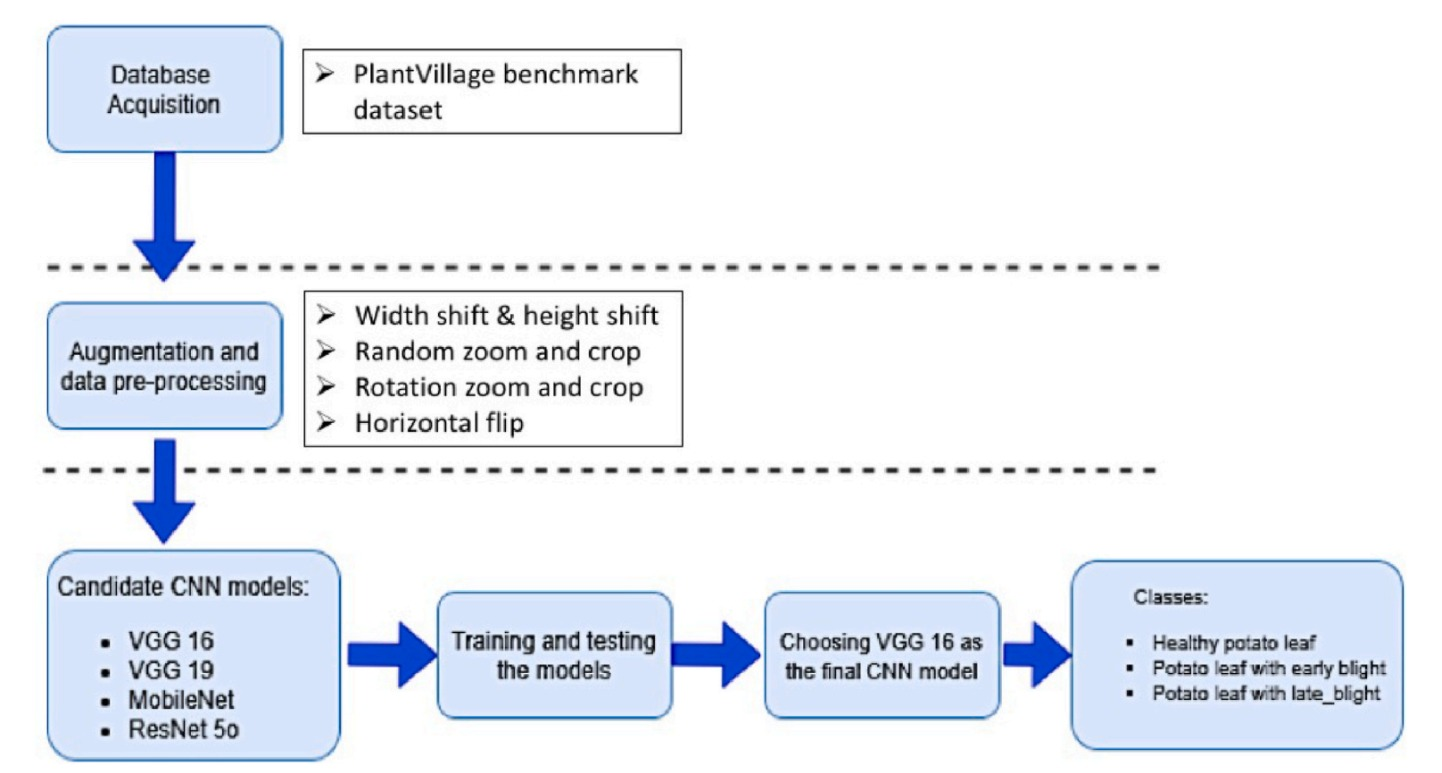
\includegraphics[width=1\textwidth]{2/figures/ant1.jpeg}
		\caption{Metodología propuesta para el modelo 
		(\cite{CHAKRABORTY2022101781})}
	\end{center}
\end{figure}

\subsubsection{Resultados obtenidos}
En el paper, cuando se evaluan las distintas técnicas de CNN a considerar, la que sobresale y tiene un mayor desempeño logrando un accuracy promedio del 92.69\%. Es por eso, que se tunea y se escoge como la técnica principal para el desarrollo del modelo final, obteniendo un accuracy promedio del 97.89\%. 
\begin{figure}[H]
	\begin{center}
		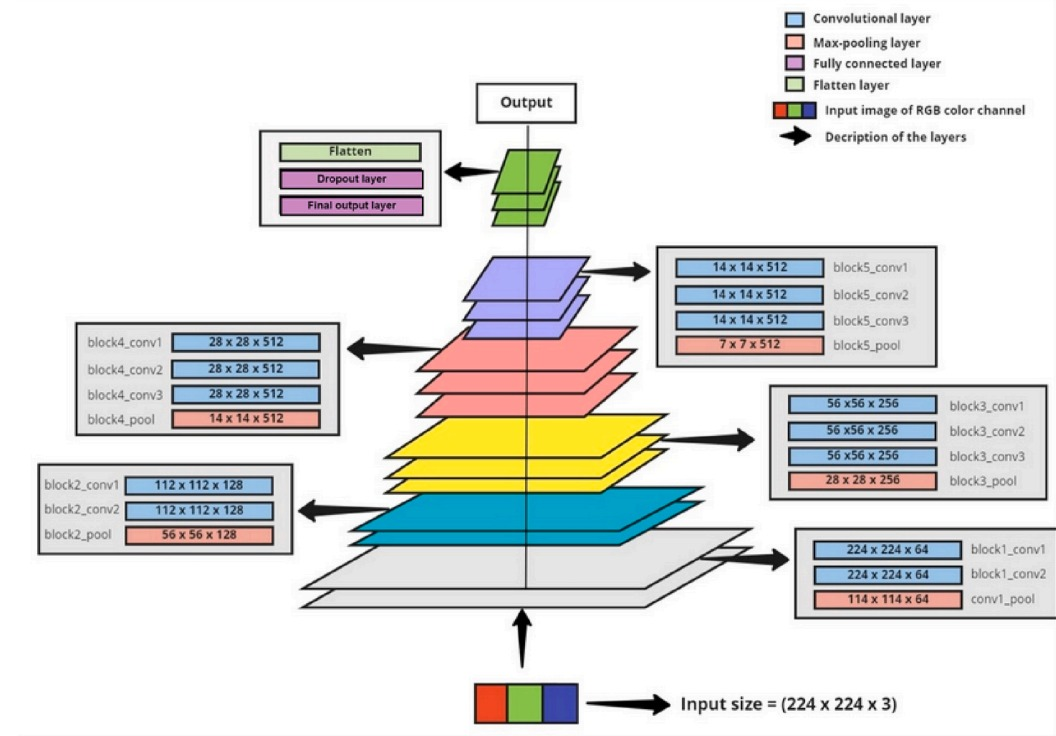
\includegraphics[width=0.8\textwidth]{2/figures/ant1.2.jpeg}
		\caption{Arquitectura del modelo ajustado propuesto de VGG16, muestra las disntitas capas (convolucion). Tambien, se mencionana los respectivos tamaños del filtro convolucional  (\cite{CHAKRABORTY2022101781})}
	\end{center}
\end{figure}

%%%%%%%%%%%%%%%%%%%%%%%%%%%%%%%%%%%%%%%%%%%%%%%%%%%%%%%%%%%%%%%%%%%%%%%%%%%%%%%%%%%%%%%%%%%%%%%%%%%%%%%%%%%%%%%%%%%%%%%%%%%%
\subsection{Research and Validation of Potato Late Blight Detection Method Based on Deep Learning \citep*{antecedente2}}

\citeauthor{antecedente2} realizó este trabajo publicado en la revista Agronomy, para la sección de Precision and Digital Agriculture.
Este fue titulado \citetitle{antecedente2} la cual traducida al español significa «Investigación y validación del método de detección del tizón tardío de la papa basado en aprendizaje profundo». La investigación nos dice que el Tizón tardío puede llevar al fracaso total del cultivo papa. Asimismo, construyeron un total de siete categorías de conjuntos de datos de enfermedades de las hojas de papa en fondos simples y complejos. Finalmente, la investigacion se introduce en diferentes modelos de Deep Learning en distantas versiones.

\subsubsection{Planteamiento del Problema y objetivo }
El trabajo discute sobre el Tizón tardío como enfermedad muy grave para los cultivos de papa. Esta pone en riesgo el total del cultivo, además que los métodos tradicionales como la detección basada en la inspección visual suele ser subjetivo y demora tiempo. Asimismo, los sistemas de detección actuales suelen ser ineficientes debido a la varibilida de luminosidad y el sombreado de las hojas. Es crucial desarrollar un modelo de detección automatizada que pueda superar estas limitaciones, permitiendo una monitorización y prevención temprana del tizón tardío de la papa. El objetivo de este estudio es desarrollar y optimizar un modelo de aprendizaje profundo para la detección del tizón tardío en hojas de papa, que sea altamente preciso y rápido en su inferencia, y que pueda ser implementado en dispositivos móviles para la monitorización automática y la alerta temprana de enfermedades en cultivos. Para alcanzar este objetivo, se plantean las siguientes metas específicas: Lograr una clasificación detallada de enfermedades, Opitmizar el modelo base elegido, Evaluar la viabilidad y efectivdad del modelo en hardware

\subsubsection{Fundamento Teórico usado por el Autor}

El autor planteó utilizar modelos de Deep Learning, se enfocó en modelos de ligeros y eficientes estos con el fin de implantar el modelo en un dispositivo móvil. Las técnicas que utilizó fueron MobileNet, ShuffleNet, GhostNet, and SqueezeNet pre-trained models usando imágenes de hojas de papa de los conjuntos de dato Plant Village y AI Challenger 2018. 


\begin{figure}[H]
	\begin{center}
		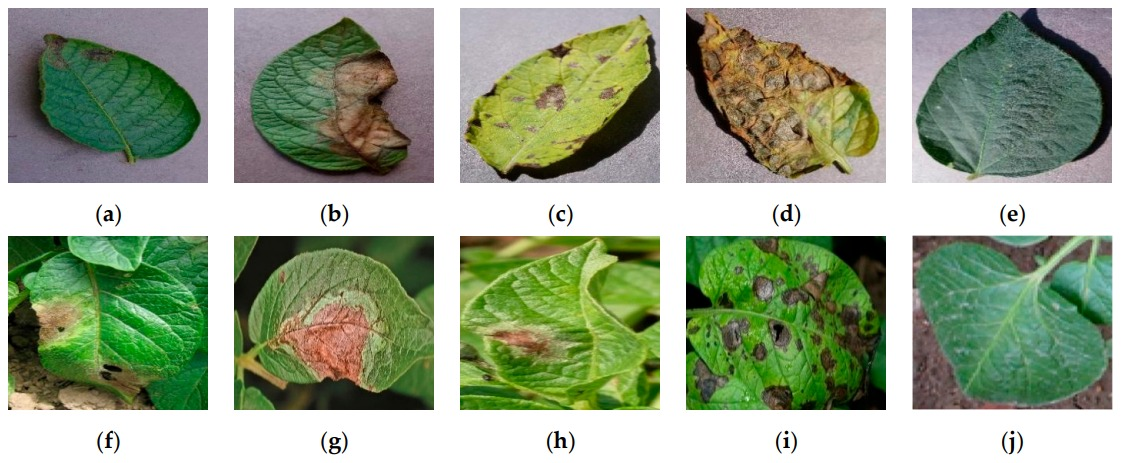
\includegraphics[width=0.6\textwidth]{2/figures/ant2.jpeg}
		\caption{ (a) Etapas tempranas de la hoja con tizón tardío en un contexto único. (b) Etapas finales de la hoja con tizón tardío en un contexto único. (c) Etapas tempranas de la hoja con tizón temprano en un contexto único. (d) Etapas finales de la hoja con tizón temprano en un contexto único. (e) Hoja sana en un contexto único. (f) Etapas tempranas de la hoja con tizón tardío en un contexto natural. (g) Etapas finales de la hoja con tizón tardío en un contexto natural. (h) Etapas tempranas de la hoja con tizón temprano en un contexto natural. (i) Etapas finales de la hoja con tizón temprano en un contexto natural. (j) Hoja sana en un contexto natural. (\cite{antecedente2})}
	\end{center}
\end{figure}


\subsubsection{Metodología empleada por los autores}
La metodología empleada por el autor, para la creación de su modelo final de clasifacion es el siguiente:


\begin{enumerate}
	\item Se adquirió la base de datos de imágenes del conjunto de datos PlantVillage y IA Challenger 2018 dataset, del cual solo extrajo imágenes de hoja de papa.
	\item Realizaron un preprocesamiento de imágenes donde usaron técnicas para la Anotación de hoja, Zona de enfermedad, Volteo de imagen, Mejora HSV, Ajuste de birllo, Agregar sombras
	\item Los CNN candidatos fueron  MobileNet, ShuffleNet, GhostNet y SqueezeNet
	\item Entrenamiento y testeo de los modelos.
	\item Se eligió ShuffleNetV2 como modelo final
	\item Las clases que el modelo clasificaba son, Hoja de papa sana, Tizón tardio nivel 1, Tizón tardio nivel 2 y Tizón tardio nivel 3
\end{enumerate}
\begin{figure}[H]
	\begin{center}
		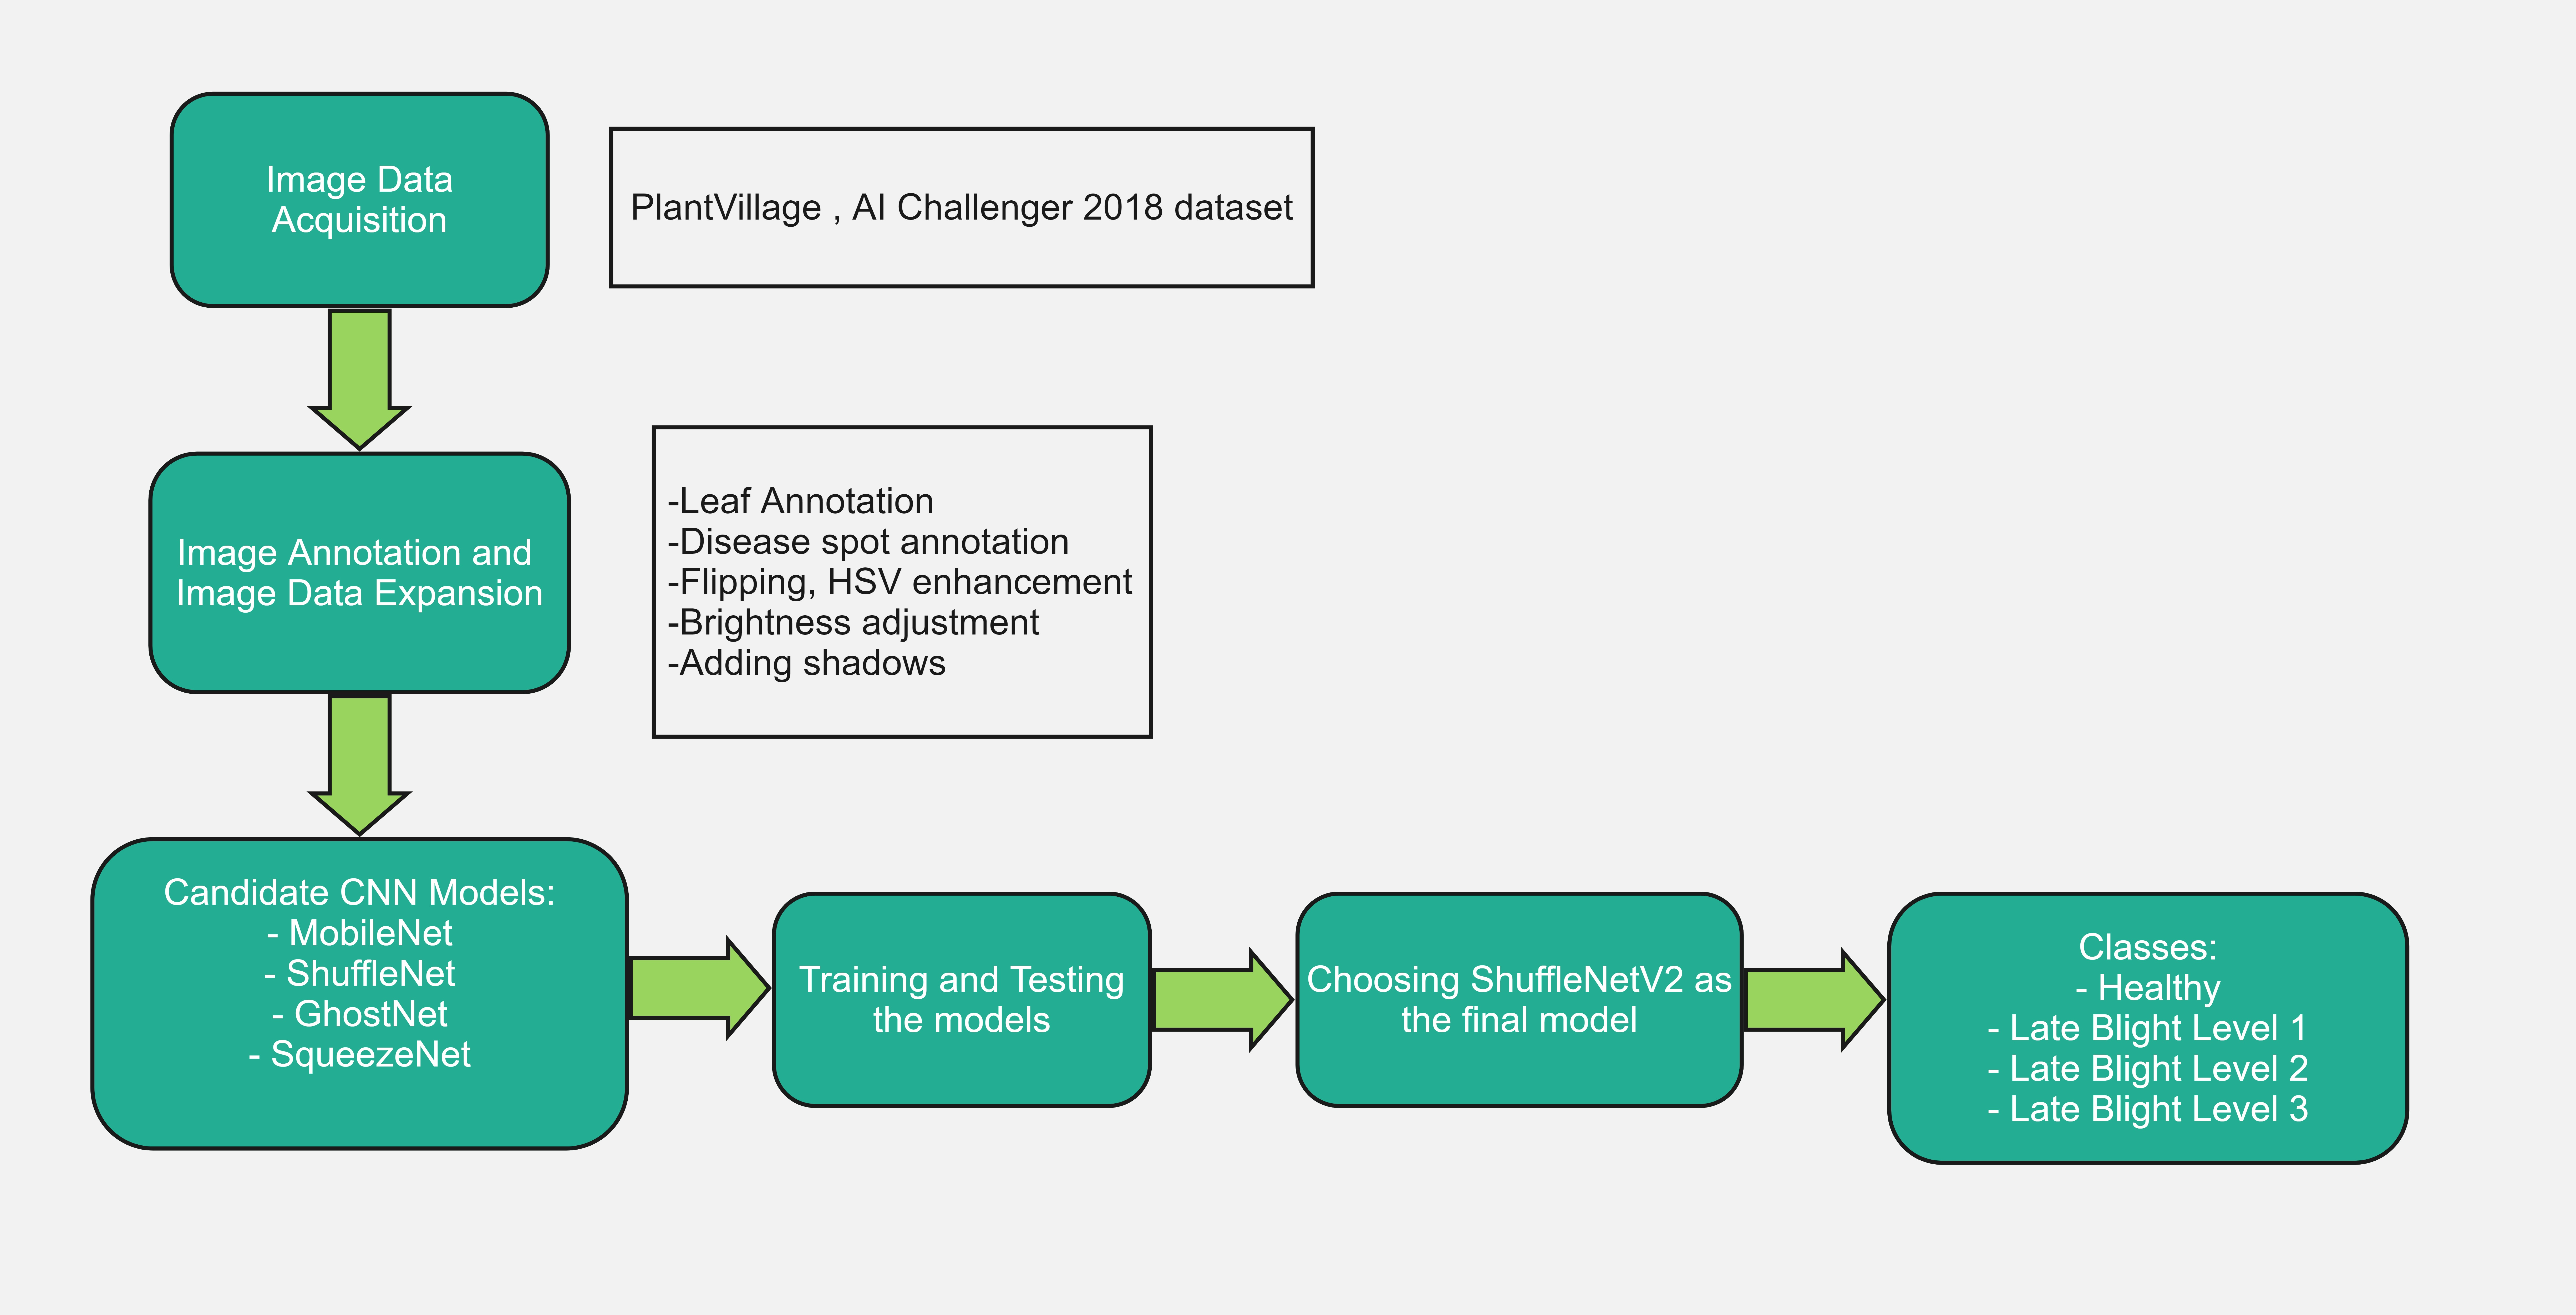
\includegraphics[width=1\textwidth]{2/figures/ant2.2.jpg}
		\caption{Arquitectura del bot de Azure (\cite{antecedente2})}
	\end{center}
\end{figure}


\subsubsection{Resultados obtenidos}
En esta investigacion, se analizaron distintos resultados con diferentes técnicas. Con la técnica final,ShuffleNetV2 , se obtuvieron resultados un accuracy de 95.41\%. Finalmente, se consideró una mejoría para esta técnica, ya que se buscaba el mejor modelo final posible para un dispositivo móvil disminuyendo el tiempo de procesamiento y el costo computacional, tomando esos objetivos en cuenta, se logró un 95.04\%

\begin{figure}[h]						
	\begin{center}
		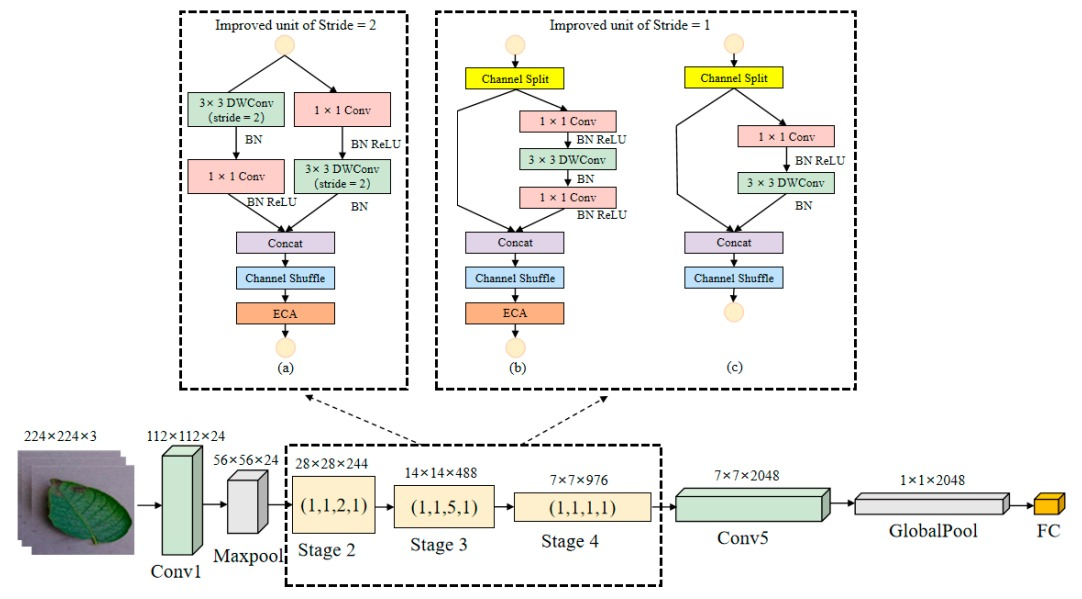
\includegraphics[width=1\textwidth]{2/figures/ant2.3.jpeg}
		\caption{Arquitectura del modelo final. 
			La estructura del modelo mejorado ShuffleNetV2 2×. Nota: La Etapa 2, la Etapa 3 y la Etapa 4 están compuestas por la unidad base original, con Stride = 1, y la unidad modificada está compuesta por una unidad con Stride = 1 y una unidad con Stride = 2. (1, 1, 2, 1) en la Etapa 2 indica una pila de la unidad (a) con Stride = 2 mejorado, una pila de la unidad (b) con Stride = 1 mejorado, dos pilas de la unidad básica con Stride = 1 original, y una pila de la unidad (c) con Stride = 1 mejorado; (1, 1, 5, 1) en la Etapa 3 indica una pila de la unidad (a) con Stride = 2 mejorado, una pila de la unidad (b) con Stride = 1 mejorado, cinco pilas de la unidad básica con Stride = 1 original, y una pila de la unidad (c) con Stride = 1 mejorado; (1, 1, 1, 1) en la Etapa 4 indica una pila de la unidad (a) con Stride = 2 mejorado, una pila de la unidad (b) con Stride = 1 mejorado, una pila de la unidad básica con Stride = 1 original, y una pila de la unidad (c) con Stride = 1 mejorado. (\cite{antecedente2})}
	\end{center}
\end{figure}
\begin{figure}[H]
	\begin{center}
		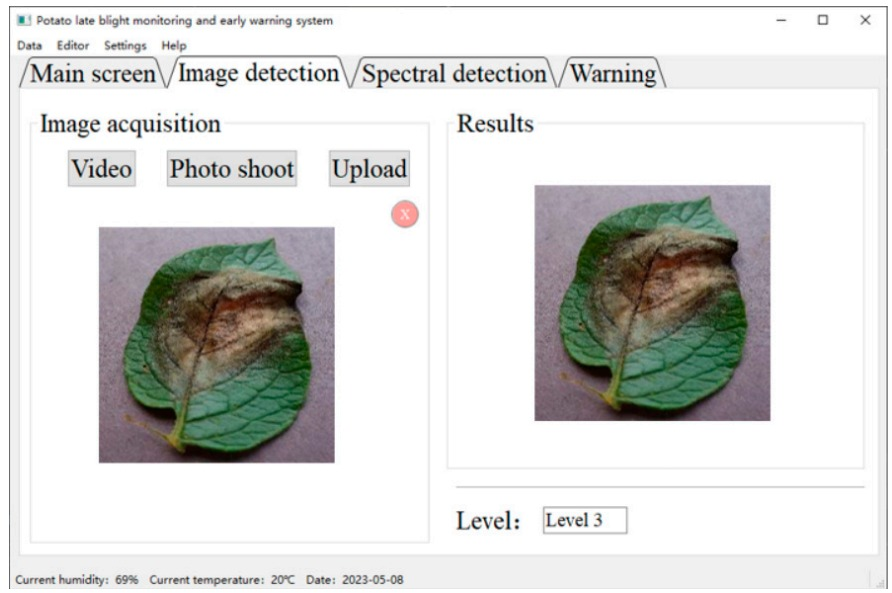
\includegraphics[width=0.7\textwidth]{2/figures/ant2.4.jpeg}
		\caption{Interfaz de operación de detección de imágenes. (\cite{antecedente2})}
	\end{center}
\end{figure}

%%%%%%%%%%%%%%%%%%%%%%%%%%%%%%%%%%%%%%%%%%%%%%%%%%%%%%%%%%%%%%%%%%%%%%%%%%%%%%%%%%%%%%%%%%%%%%%%%%%%%%%%%%%%%%%%%%%%%%%%%%%%


\subsection{Supervised Learning-Based Image Classification for the Detection of Late Blight in Potato Crop \citep*{antecedente3}}

\citeauthor{antecedente3} realizó un trabajo con el fin de ser publicado en la revista Computer Vision and Pattern Recognition Based on Deep Learning. Este fue titulado \citetitle{antecedente3} la cual traducida al español significa  «Clasificación de imágenes basada en aprendizaje supervisado para la detección del tizón tardío en cultivos de papa». La investigación plantea el desarrollo de un modelo de detección temprana del Tizón tardío en la papa utilizando Redes Neuronales Convolucionales y Máquinas de Vectores de Soporte. Asimismo, el autor desarrolló, por sí mismo, su base de datos de imágenes de cultivos de papa. Finalmente, se aplicaron varias métricas de rendimiento, eficiencia y calidad en las tareas de aprendizaje y clasificación para determinar los mejores algoritmos de aprendizaje automático.

\subsubsection{Planteamiento del Problema y objetivo }

La investigación aborda la necesidad de encontrar métodos más eficaces en cuanto a la detección temprana del Tizón Tardío causada por Oomiceto Phytophthora, que afecta rápidamente las hojas, tallos y tubérculos de la papa que es un alimento crucial en la economía de Bógota. Asimismo, la detección tradicional, como pruebas de laboratorio, aunque es eficaz, toma mucho tiempo y es altamente costoso. En conlusión, el objetivo principal del estudio es aplicar técnicas de aprendizaje supervisado y clasificación de imágenes, específicamente mediante redes neuronales convolucionales (CNN) y máquinas de vectores de soporte (SVM), para la detección temprana del tizón tardío en cultivos de papa.

\subsubsection{Fundamento Teórico usado por el Autor}

El autor plantea hacer uso de CNN y SVM como sus posibles modelos finales. Utiliza una CNN, según el preprocesamiento de la data, no modificada y una aumentada, por otro lado, divide SVM en cuatro posibles modelos según caracteristica del preprocesamiento: Color, Textura, PCA, Combined. 

\subsubsection{Metodología empleada por los autores}
La metodología empleada por el autor, para la creación de su modelo consiste en los siguientes pasos: 

\begin{enumerate}
	\item Captura los datos imputados por parte del cliente.
	\item Envía el query a Dialogflow para su procesamiento.
	\item Se procesa la información mediante una API externa y el código implementado, así como la base de datos.
	\item Retorna los resultados procesados y se agrega información extra requerida.
	\item Envía al cliente o usuario la respuesta.
\end{enumerate}

\begin{figure}[H]
	\begin{center}
		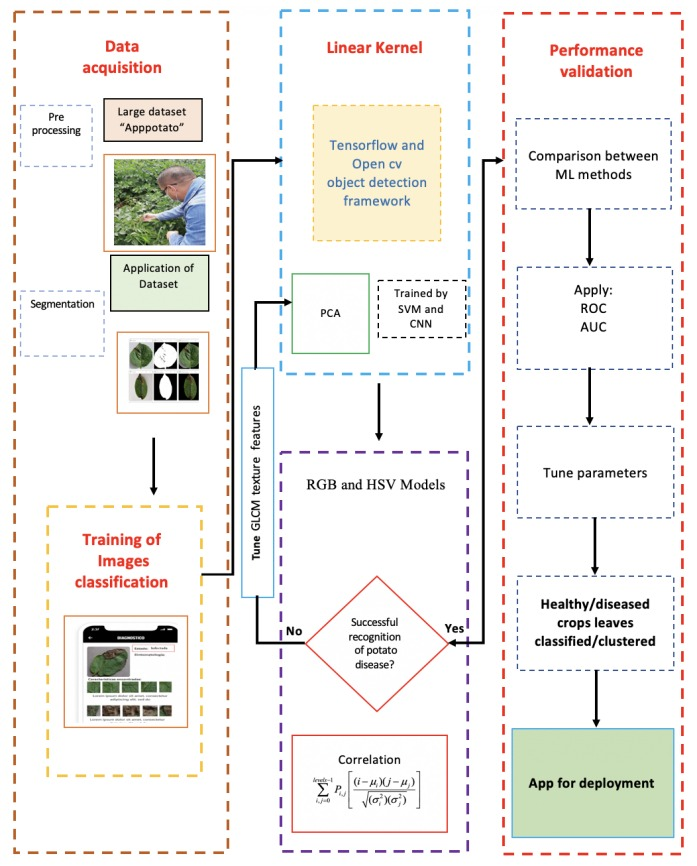
\includegraphics[width=1\textwidth]{2/figures/ant3.jpeg}
		\caption{Diagrama de la metodologia Flowchart(\cite{antecedente3})}
	\end{center}
\end{figure}

\subsubsection{Resultados obtenidos}

Las CNN entrenadas con el conjunto de datos aumentado mostraron el mejor desempeño con una precisión del 93\% y una AUC de 0.97. Además, las SVM entrenadas con características de color obtuvieron mejores resultados en comparación con las SVM entrenadas con otras características. Finalmente, se propone desarrollar una aplicación móvil con características avanzadas para la agricultura de precisión que ayude a los agricultores a identificar la enfermedad del tizón tardío de manera no invasiva y en tiempo real..

%%%%%%%%%%%%%%%%%%%%%%%%%%%%%%%%%%%%%%%%%%%%%%%%%%%%%%%%%%%%%%%%%%%%%%%%%%%%%%%%%%%%%%%%%%%%%%%%%%%%%%%%%%%%%%%%%%%%%%%%%%%%
\subsection{Potato Blight Classification Android Application using Deep Learning  \citep*{antecedente5}}

\citeauthor{antecedente5} realizó un artículo publicado en base de datos de ELSEVIER, siendo también parte de la revista Sustainable Chemistry and Pharmacy en el año 2022. Este fue titulado \citetitle{antecedente5} la cual traducida al español significa «Redes neuronales convolucionales profundas para la detección de enfermedades de la hoja del tomate basada en imágenes». El trabajo nos dice que el reconocimiento de enfermedades foliares en las plantas representa un riesgo significativo para la seguridad alimentaria, ya que puede reducir la producción agrícola y, por ende, la economía nacional. Es crucial identificar estas enfermedades en etapas tempranas para mejorar la calidad y cantidad de los productos agrícolas. Por lo tanto, se requiere un sistema automático de reconocimiento de enfermedades foliares que pueda identificar y clasificar estas enfermedades en etapas tempranas. En este contexto, se han utilizado modelos de redes neuronales convolucionales profundas (DCNN) para el análisis de imágenes de hojas, con el objetivo de mejorar la precisión y reducir el tiempo de respuesta en la identificación de enfermedades foliares en tomates. Se propone un sistema automático de identificación de enfermedades foliares en tomates utilizando DCNN, con un conjunto de datos de 18160 imágenes de hojas de tomate. Este conjunto de datos se dividió en un 60\% para entrenamiento y un 40\% para pruebas, logrando una precisión del 98.40\% en el conjunto de pruebas con el modelo DCNN propuesto.

\subsubsection{Planteamiento del Problema y objetivo }

El artículo aborda principalmente que las enfermedades en las hojas de tomate causan pérdidas significativas en la producción, afectando tanto la calidad como la cantidad de los productos. Identificar y diagnosticar estas enfermedades de manera temprana es crucial, ya que pueden reducir drásticamente el crecimiento de los cultivos y, por lo tanto, la producción. Sin embargo, el diagnóstico manual de las enfermedades foliares puede llevar a una disminución en la producción debido a la gravedad de las enfermedades y a la variabilidad en los síntomas causada por factores ambientales como la temperatura, el viento y la humedad. Por lo tanto, existe una necesidad de desarrollar un sistema automático que pueda identificar y diagnosticar estas enfermedades en etapas tempranas, permitiendo a los agricultores tomar medidas preventivas adecuadas para proteger sus cultivos. El objetivo es desarrollar una herramienta automática que diagnostique las enfermedades de las hojas de tomate tempranamente para mejorar la producción agrícola. Se utilizará un enfoque basado en redes neuronales convolucionales profundas (DCNN) para clasificar 10 tipos de enfermedades en los cultivos de tomate, con el fin de identificar los síntomas de las hojas en etapas tempranas y mejorar la eficiencia y precisión del modelo mediante técnicas de ajuste de parámetros.

\subsubsection{Fundamento Teórico usado por el Autor}

Los autores plantean utilizar como técnica principal una DCNN (Deep Convolutional Neural Networks) y compararla con técnicas como MLP (Multiplayer Layer Perceptron) y SVM (Support Vector Machine).



\subsubsection{Metodología empleada por los autores}
La metodología empleada por los autores, para la creación de su chatbot consiste en los siguientes pasos: 
\begin{enumerate}
	\item Se adquirió la base de datos de imágenes del conjunto de datos PlantVillagey
	\item Realizaron un preprocesamiento de imágenes donde se ajusto el tamaño de imagenes.
	\item El modelo utilizó una DCNN
	\item Entrenamiento y testeo de los modelos.
	\item Se reajusto el modelo
	\item Finalmente se compararon los resultados del modelo final con MLP y SVM
\end{enumerate}
\begin{figure}[H]
	\begin{center}
		
\includegraphics[width=1\textwidth]{2/figures/ant5.jpg}
		\caption{Metodología (\cite{antecedente5})}
	\end{center}
\end{figure}

\subsubsection{Resultados obtenidos}
Como resultado del desarrollo del modelo final, este alcanzó un 98.40\% de accuracy promedio, mientras que SVM obtuvo un accuracy de 90.01\% y MLP un accuracy de 88.30\%. 

\begin{figure}[H]
	\begin{center}
		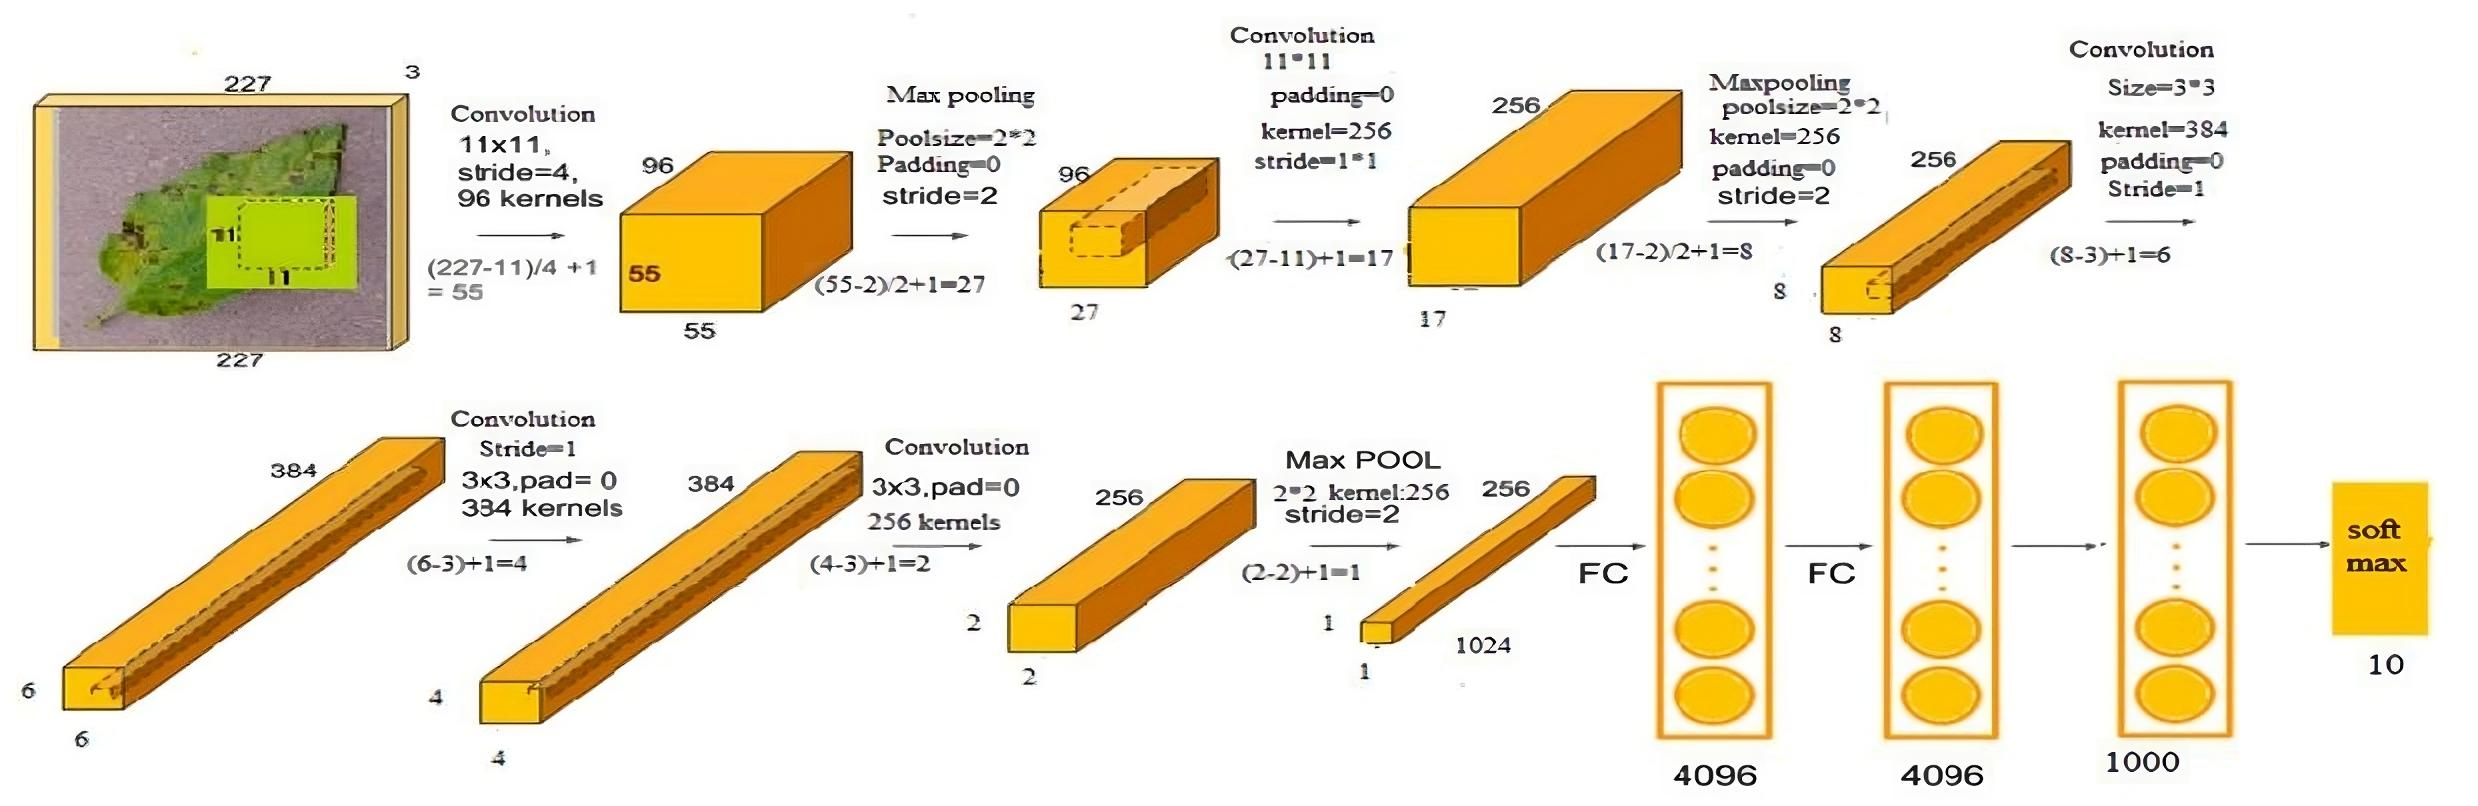
\includegraphics[width=1\textwidth]{2/figures/ant5.2.jpeg}
		\caption{Arquitectura del modelo final (\cite{antecedente5})}
	\end{center}
\end{figure}
%%%%%%%%%%%%%%%%%%%%%%%%%%%%%%%%%%%%%%%%%%%%%%%%%%%%%%%%%%%%%%%%%%%%%%%%%%%%%%%%%%%%%%%%%%%
%%%%%%%%%%%%%%%%%%%%%%%%%%%%%%%%%%%%%%%%%%%%%%%%%%%%%%%%%%%%
\subsection{Deep Convolutional Neural Networks for image based tomato leaf disease detection  \citep*{antecedente6}}

\citeauthor{antecedente6} realizó un artículo publicado en base de datos de International Journal of Advanced Research in Science, Communication and Technology (IJARSCT) en el año 2023. Este fue titulado \citetitle{antecedente6} la cual traducida al español significa «Aplicación para Android de clasificación del tizón de la papa usando el aprendizaje profundo». La investigación sostiene que los agricultores de papas sufren pérdidas económicas debido a enfermedades como el tizón temprano y tardío. La detección temprana y tratamiento adecuado pueden prevenir estas pérdidas, pero los métodos tradicionales son lentos y propensos a errores. Proponemos usar una Red Neuronal Convolucional (CNN) personalizada para diagnosticar enfermedades de plantas de manera rápida y precisa, reduciendo el tiempo de computación y minimizando errores, lo que ayuda a los agricultores a tratar las enfermedades a tiempo y reducir pérdidas.

\subsubsection{Planteamiento del Problema y objetivo }
El trabajo sustenta que la industria de la papa enfrenta un desafío significativo en la prevención de pérdidas de cultivos debido a enfermedades como el tizón temprano y el tizón tardío. Estas enfermedades pueden causar pérdidas económicas sustanciales para los agricultores si no se detectan y tratan a tiempo. Los métodos tradicionales de inspección visual son lentos, propensos a errores y no son viables para aplicaciones en tiempo real debido a los largos tiempos de procesamiento de imágenes. Además, existe la necesidad de mejorar la precisión y reducir el tiempo de computación en los métodos actuales de diagnóstico de enfermedades de las plantas. Por eso, su objetivo es desarrollar una red neuronal convolucional (CNN) eficiente y precisa para detectar enfermedades en las plantas de papa, reduciendo el tiempo de computación y mejorando la precisión, con el fin de ayudar a los agricultores a tratar las enfermedades a tiempo y reducir pérdidas económicas. 

\subsubsection{Fundamento Teórico usado por el Autor}

Los autores formulan utilizar como técnica principal un Red Neuronal Convolucional, mejorarla para que sea una Red neuronal convolucional personalizada de enfermedades profundas (PDDCNN), ya que buscan lograr un modelo que se adapte a distintas regiones de donde se pueda obtener el dataset.


\subsubsection{Metodología empleada por los autores}
La metodología empleada por los autores, para la creación de su chatbot consiste en los siguientes pasos: 
\begin{enumerate}
	\item Se adquirió la base de datos de imágenes del conjunto de datos PlantVillage. Asimismo, añadieron una base de datos de imagenes propias tomadas con camaras digitales
	\item Realizaron un preprocesamiento de imágenes donde se ajusto el tamaño de imagenes segun el dataset..
	\item El modelo utilizó una CNN
	\item Entrenamiento y testeo de los modelos.
	\item Se reajusto el modelo a una PDDCNN
	\item Finalmente, el modelo final detecto las clases Tizon Temprao, Tizon Tardio, Hoja Saludable
\end{enumerate}
\begin{figure}[H]
	\begin{center}
		
\includegraphics[width=1\textwidth]{2/figures/ant6.jpg}
		\caption{Metodología (\cite{antecedente6})}
	\end{center}
\end{figure}

\subsubsection{Resultados obtenidos}
Los resultados finales fueron tomados sobre la base de datos que ellos crearon después de entrenar su modelo con el conjunto de datos PlantVillage. Obtuvo un accuracy de 99\% en el tizon tardio y tizon temprano, mientras que en las hojas sanas tuvieron un accuracy de 100\% 

\begin{figure}[H]
	\begin{center}
		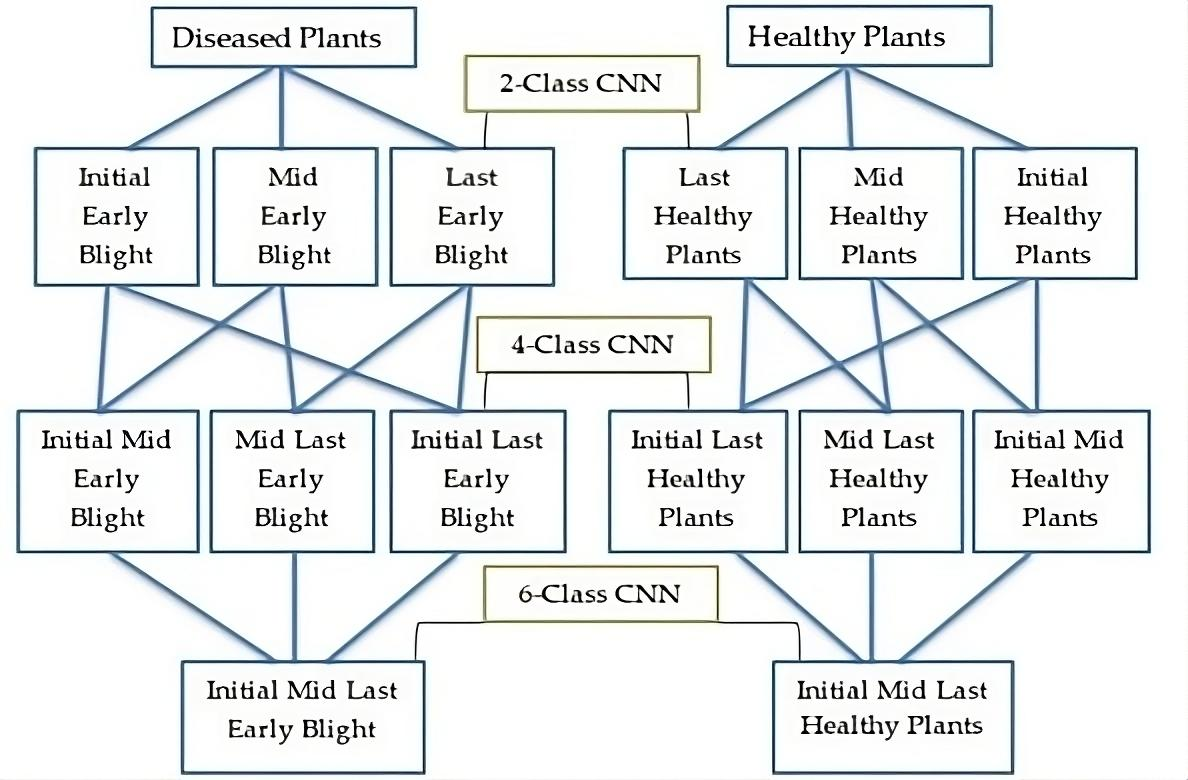
\includegraphics[width=1\textwidth]{2/figures/ant6.2.jpeg}
		\caption{Arquitectura del modelo final (\cite{antecedente6})}
	\end{center}
\end{figure}
%%%%%%%%%%%%%%%%%%%%%%%%%%%%%%%%%%%%%%%%%%%%%%%%%%%%%%%%%%%%%%%%%%%%%%%%%%%%%%%%%%%%%%%%%%%%%%%%%%%%%%%%%%%%%%%%%%%%%%%%%%%%%%
\subsection{Potato Blight Classification Android Application using Deep Learning  \citep*{antecedente7}}

\citeauthor{antecedente7} realizó un artículo publicado en base de datos de ELSEVIER, siendo también parte de la revista Sustainable Chemistry and Pharmacy en el año 2022. Este fue titulado \citetitle{antecedente7} la cual traducida al español significa «Redes neuronales convolucionales profundas para la detección de enfermedades de la hoja del tomate basada en imágenes». El trabajo nos dice que el reconocimiento de enfermedades foliares en las plantas representa un riesgo significativo para la seguridad alimentaria, ya que puede reducir la producción agrícola y, por ende, la economía nacional. Es crucial identificar estas enfermedades en etapas tempranas para mejorar la calidad y cantidad de los productos agrícolas. Por lo tanto, se requiere un sistema automático de reconocimiento de enfermedades foliares que pueda identificar y clasificar estas enfermedades en etapas tempranas. En este contexto, se han utilizado modelos de redes neuronales convolucionales profundas (DCNN) para el análisis de imágenes de hojas, con el objetivo de aumentar la exactitud y disminuir el tiempo de respuesta. identificación de enfermedades foliares en tomates. Se propone un sistema automático de identificación de enfermedades foliares en tomates utilizando DCNN, con un conjunto de datos de 18160 imágenes de hojas de tomate. Este conjunto de datos se dividió en un 60\% para entrenamiento y un 40\% para pruebas, logrando una precisión del 98.40\% en el conjunto de pruebas con el modelo DCNN propuesto.

\subsubsection{Planteamiento del Problema y objetivo }

El artículo aborda principalmente que las enfermedades en las hojas de tomate causan pérdidas significativas en la producción, afectando tanto la calidad como la cantidad de los productos. Identificar y diagnosticar estas enfermedades de manera temprana es crucial, ya que pueden reducir drásticamente el crecimiento de los cultivos y, por lo tanto, la producción. Sin embargo, el diagnóstico manual de las enfermedades foliares puede llevar a una disminución en la producción debido a la gravedad de las enfermedades y a la variabilidad en los síntomas causada por factores ambientales como la temperatura, el viento y la humedad. Por lo tanto, existe una necesidad de desarrollar un sistema automático que pueda identificar y diagnosticar estas enfermedades en etapas tempranas, permitiendo a los agricultores tomar medidas preventivas adecuadas para proteger sus cultivos. El objetivo es desarrollar una herramienta automática que diagnostique las enfermedades de las hojas de tomate tempranamente para mejorar la producción agrícola. Se utilizará un enfoque basado en redes neuronales convolucionales profundas (DCNN) para clasificar 10 tipos de enfermedades en los cultivos de tomate, con el fin de identificar los síntomas de las hojas en etapas tempranas y mejorar la eficiencia y precisión del modelo mediante técnicas de ajuste de parámetros.

\subsubsection{Fundamento Teórico usado por el Autor}

Los autores plantean utilizar como técnica principal una DCNN (Deep Convolutional Neural Networks) y compararla con técnicas como MLP (Multiplayer Layer Perceptron) y SVM (Support Vector Machine).

\subsubsection{Metodología empleada por los autores}
La metodología empleada por los autores, para la creación de su modelo consiste en los siguientes pasos: 
\begin{enumerate}
	\item Se adquirió la base de datos de imágenes del conjunto de datos PlantVillage.
	\item Realizaron un preprocesamiento de imágenes donde se hizo el labeling manualmente.
	\item Se extrajo caracteristicas de las imagenes usando VGG19
	\item Los candidatos de CNN para esta investigacion fueron VGG16, VGG19 e Inception v3
	\item Se hizo el testeo y entrenamiento del modelo
	\item Finalmente, se evaluó el modelo con las siguientes metricas: AUC, CA, F1, Precision y Recall
\end{enumerate}
\begin{figure}[H]
	\begin{center}
		
\includegraphics[width=1\textwidth]{2/figures/ant7.jpg}
		\caption{Metodología (\cite{antecedente7})}
	\end{center}
\end{figure}

\subsubsection{Resultados obtenidos}
Para escoger su modelo consideraron VGG19 con la técnica de clasificación Logistic Regresion. Este alcanzó 97.8\% de accuracy sobre el testeo del dataset. 

\begin{figure}[H]
	\begin{center}
		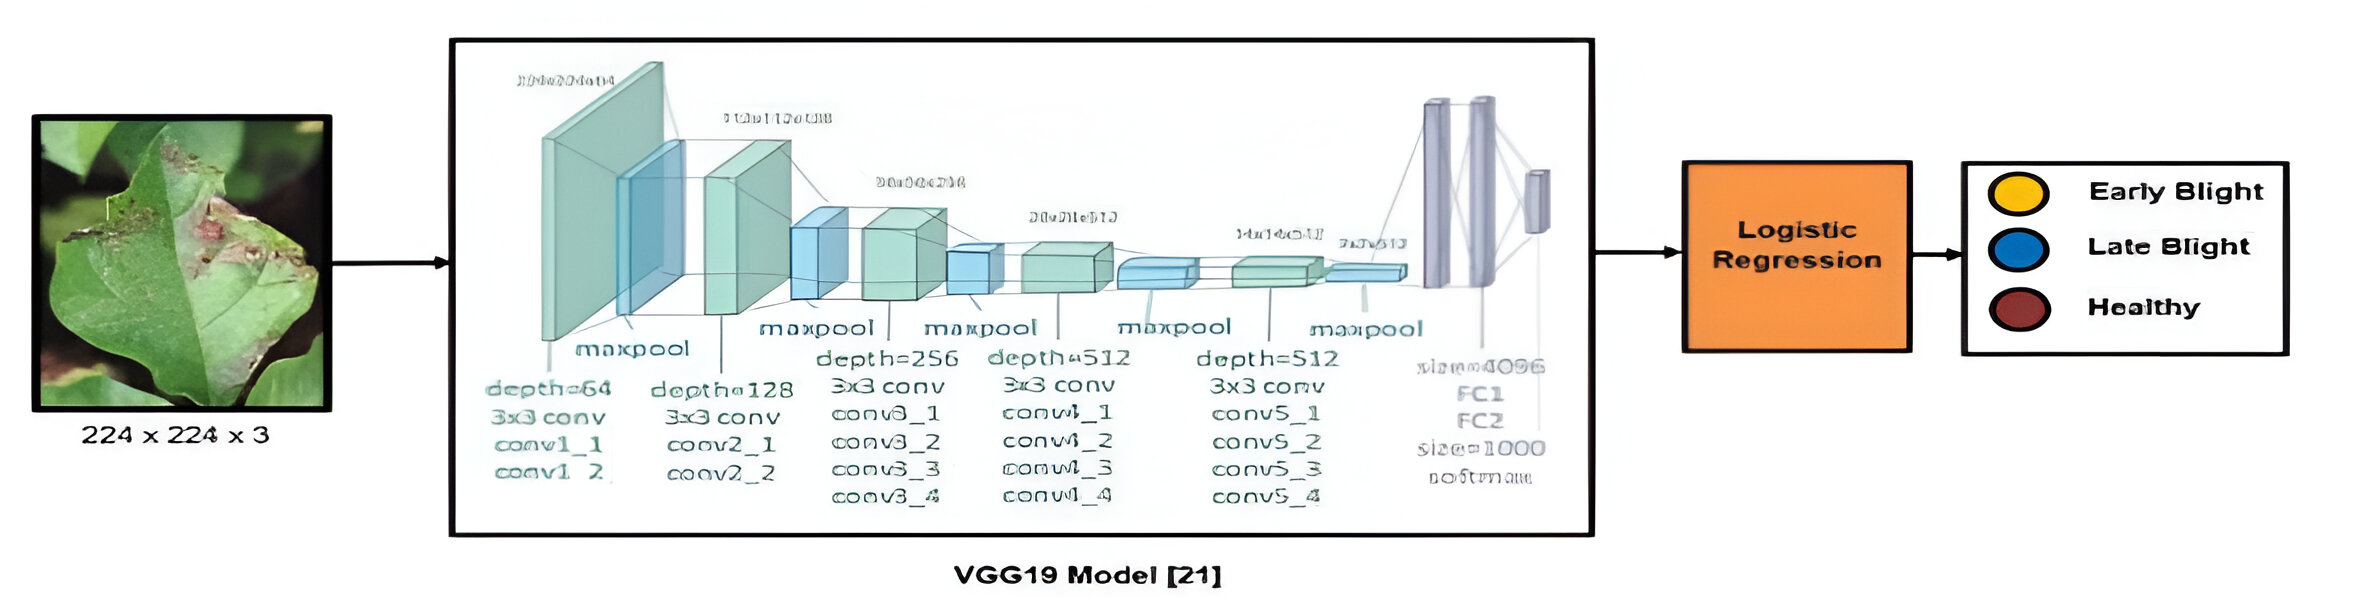
\includegraphics[width=1\textwidth]{2/figures/ant7.2.jpeg}
		\caption{Arquitectura del modelo final (\cite{antecedente7})}
	\end{center}
\end{figure}
%%%%%%%%%%%%%%%%%%%%%%%%%%%%%%%%%%%%%%%%%%%%%%%%%%%%%%%%%%%%%%%%%%%%%%%%%%%%%%%%%%%%%%%%%%%%%%%%%%%%%%%%%%%%%%%%%%%%%%%%%%%%%%
\subsection{Investigation of Phytophthora Infestans Causing Potato Late Blight Disease: A Review \citep*{antecedente4}}

\citeauthor{antecedente4} realizó un trabajo con el fin de ser publicado en la revista Biomedicine and Chemical Sciences. Este fue titulado \citetitle{antecedente4} la cual traducida al español significa  «Investigación de Phytophthora Infestans que causa el tizón tardío de la papa». La investigación sostiene Phytophthora infestans causa el tizón tardío de la papa, infectando raíces, tubérculos y brotes. La propagación se debe al cultivo de tubérculos infectados y restos de plantas en el campo. Las estructuras como micelio, zoosporas, oosporas y esporangios pueden causar infección, y las oosporas pueden sobrevivir de 3 a 4 años en bajas temperaturas. P. infestans puede causar pérdidas de hasta el 100\% en condiciones óptimas. Hay dos patrones de apareamiento, A1 y A2, y varios patrones genéticos que complican el control de la enfermedad. Las estrategias de control incluyen químicos, rotación de cultivos, agentes biológicos y plantas resistentes, siendo más efectivo combinar plantas resistentes y fungicidas. El artículo analiza los factores de propagación y desafíos del tizón tardío.
\subsubsection{Planteamiento del Problema y objetivo }

La investigación aborda que el hongo Phytophthora sp, con más de 60-80 especies, infecta diversas plantas, incluidas las papas y los tomates. Phytophthora infestans, en particular, causa estragos en estos cultivos, provocando pérdidas significativas de rendimiento y desencadenando eventos históricos como la hambruna irlandesa en la década de 1840. A pesar de los esfuerzos de control, la enfermedad del tizón tardío sigue siendo una amenaza global para la producción de papas, con pérdidas que pueden variar del 50 al 100\% dependiendo de diversos factores ambientales y de gestión. El objetivo principal es investigar Phytophthora infestans y su impacto en la enfermedad del tizón tardío en las papas. Se busca comprender mejor los modos de infección, las estrategias de reproducción del patógeno y los factores que contribuyen a su agresividad. A través de esta investigación, se espera identificar mejores métodos de control y gestión de la enfermedad, incluyendo el uso de fungicidas, prácticas culturales y la resistencia de las plantas hospederas, para mitigar las pérdidas económicas y asegurar la seguridad alimentaria en las regiones afectadas.

\subsubsection{Fundamento Teórico usado por el Autor}

El autor desarrolla su investigación en base a múltiples investigaciones pasadas. Desde los orígenes del Tizón tardío, hasta su condición en el mundo actual.

\subsubsection{Metodología empleada por los autores}
La metodología empleada por el autor, para la creación de su chatbot consiste en los siguientes pasos: 


\begin{figure}[H]
	\begin{center}
		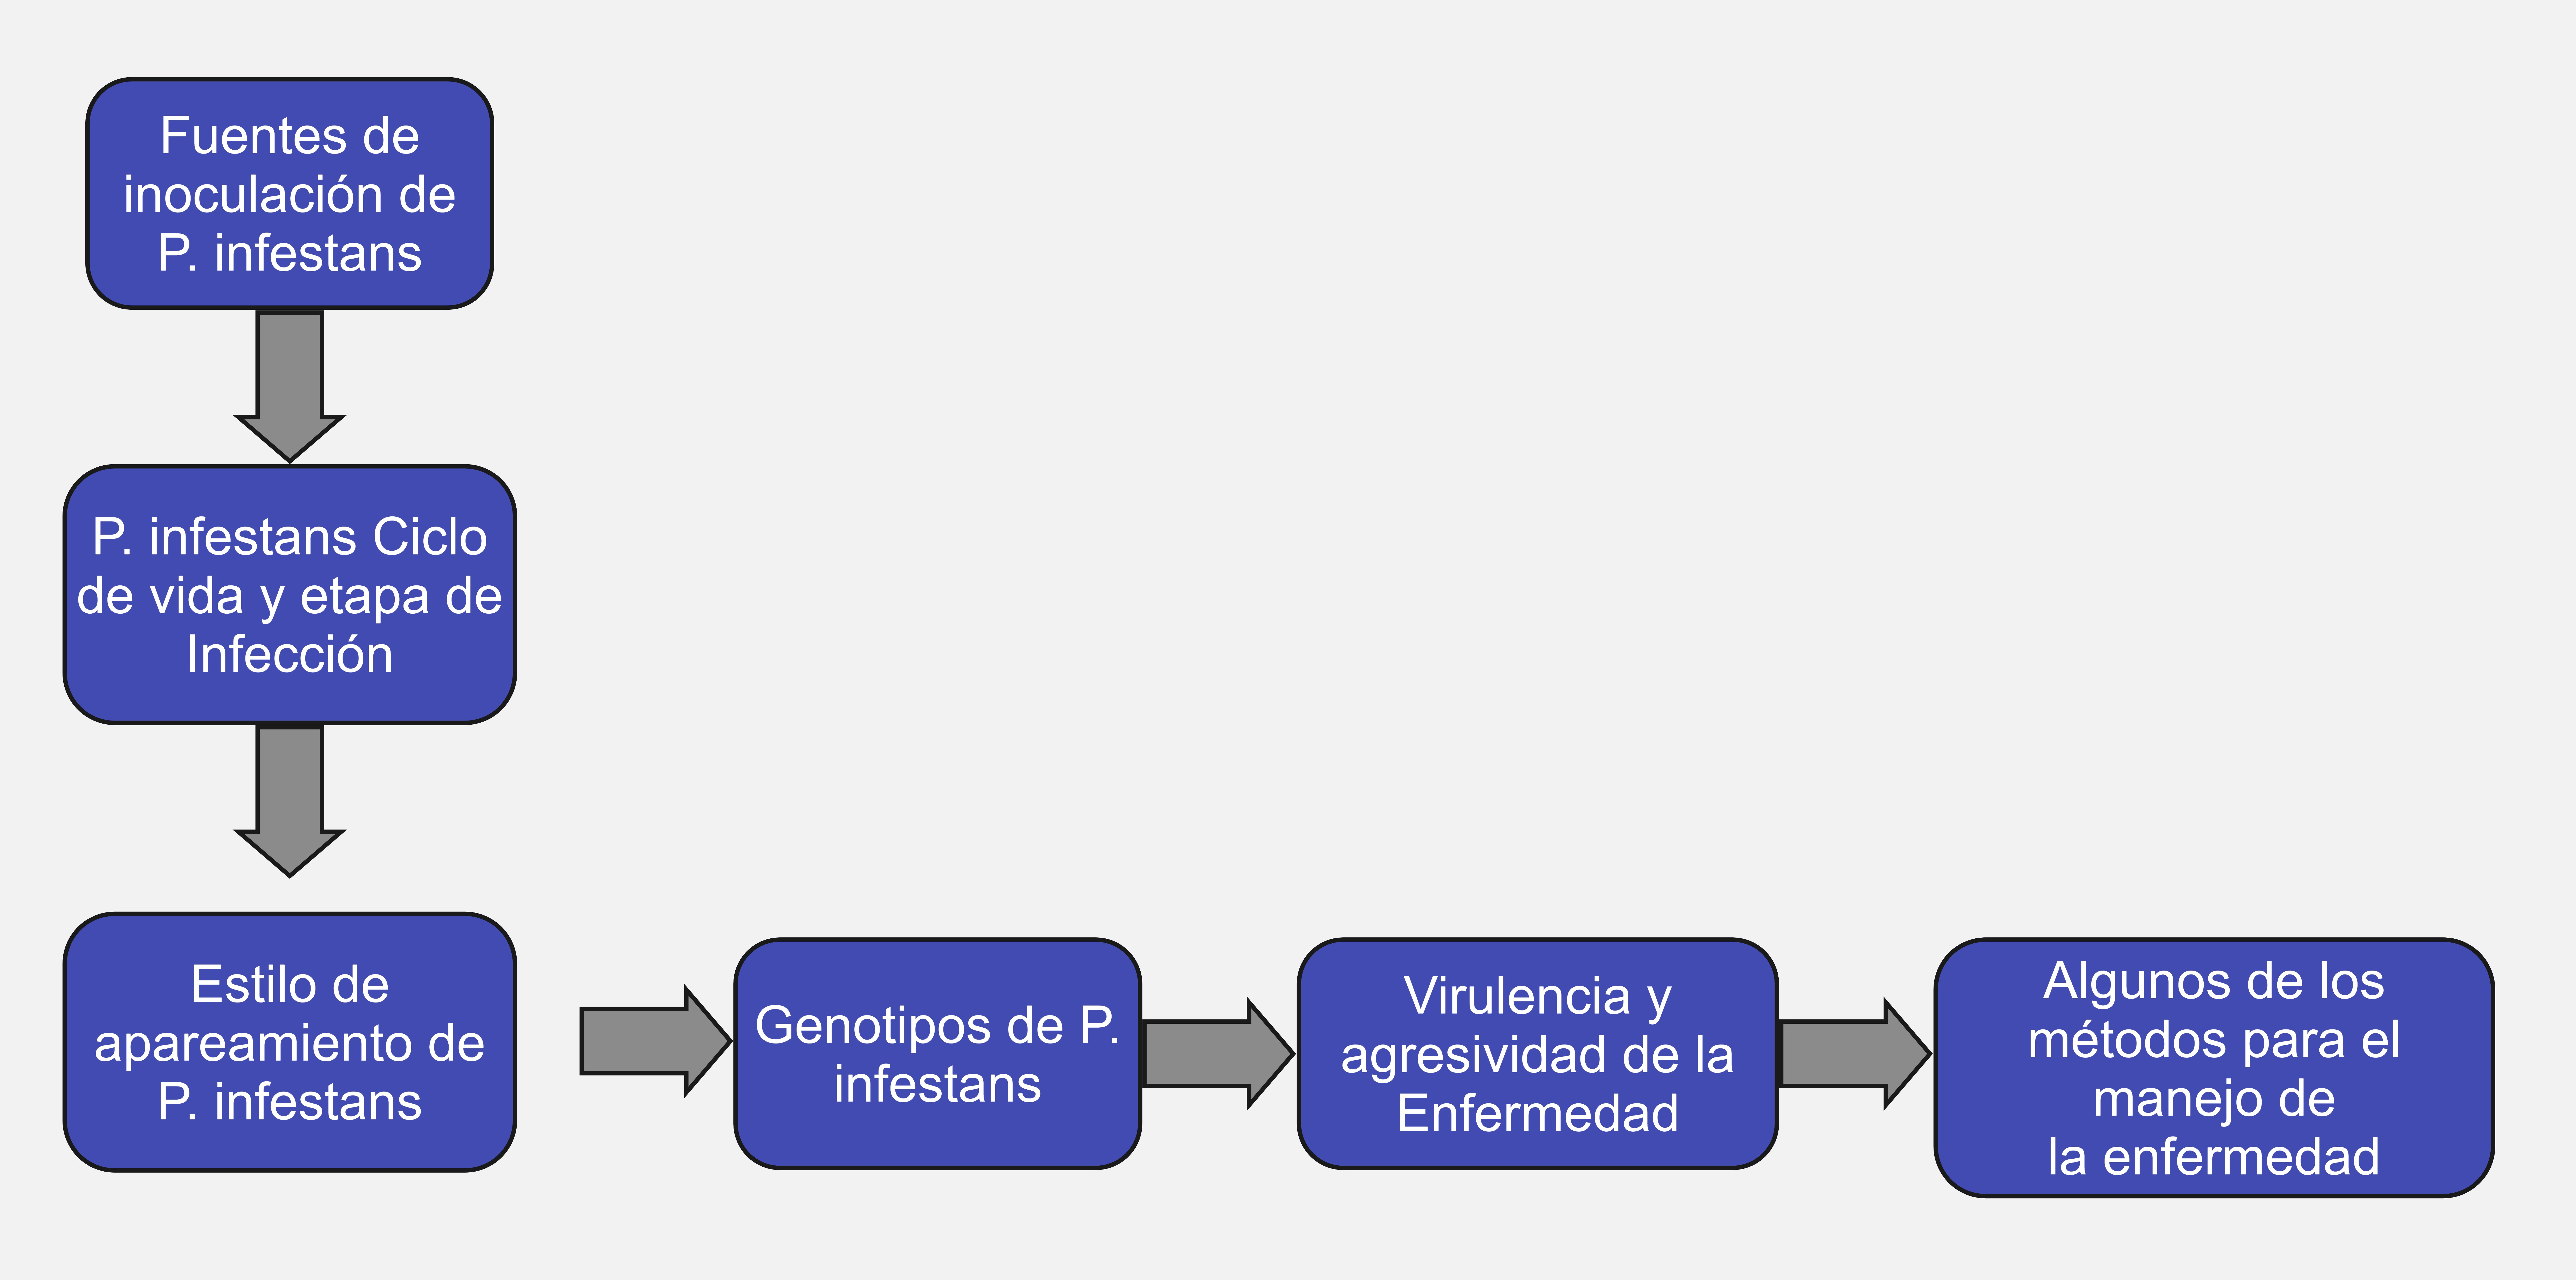
\includegraphics[width=1\textwidth]{2/figures/ant4.jpg}
		\caption{Diagrama de la metodologia(\cite{antecedente4})}
	\end{center}
\end{figure}

\subsubsection{Resultados obtenidos}

Los aislamientos de P. infestans tienen varias estructuras de infección que pueden infectar diferentes partes de la planta de papa y pueden sobrevivir durante un largo período. El hongo es capaz de reproducirse tanto sexual como asexualmente, y también presenta patrones de apareamiento A1 y A2 y diferentes genotipos. Todas estas características han llevado a la aparición de varios desafíos en el estudio de la virulencia y la agresividad. El segundo y más importante desafío incluye cómo elegir el mejor método para controlar la enfermedad (tizón tardío), ya que aparecen aislamientos que pueden resistir diferentes fungicidas, también pueden infectar plantas resistentes y muchas razones hacen que este desafío sea más relevante.

%%%%%%%%%%%%%%%%%%%%%%%%%%%%%%%%%%%%%%%%%%%%%%%%%%%%%%%%%%%%%%%%%%%%%%%%%%%%%%%%%%%%%%%%%%%%%%%%%%%%%%%%%%%%%%%%%%%%%%%%%%%%




%%%%%%%%%%%%%%%%%%%%%%%%%%%%%%%%%%%%%%%%%%%%%%%%%%%%%%%%%%%%%%%%%%%%%%%%%%%%%%%%%%%%%%%%%%%%%%%%%%%%%%%%%%%%%%%%%%%%%%%%%%%%

%%%%%%%%%%%%%%%%%%%%%%%%%%%%%%%%%%%%%%%%%%%%%%%%%%%%%%%%%%%%%%%%%%%%%%%%%%%%%%%%%%%%%%%%%%%%%%%%%%%%%%%%%%%%%%%%%%%%%%%%%%%%

%%%%%%%%%%%%%%%%%%%%%%%%%%%%%%%%%%%%%%%%%%%%%%%%%%%%%%%%%%%%%%%%%%%%%%%%%%%%%%%%%%%%%%%%%%%%%%%%%%%%%%%%%%%%%%%%%%%%%%%%%%%%

%%%%%%%%%%%%%%%%%%%%%%%%%%%%%%%%%%%%%%%%%%%%%%%%%%%%%%%%%%%%%%%%%%%%%%%%%%%%%%%%%%%%%%%%%%%%%%%%%%%%%%%%%%%%%%%%%%%%%%%%%%%%

%%%%%%%%%%%%%%%%%%%%%%%%%%%%%%%%%%%%%%%%%%%%%%%%%%%%%%%%%%%%%%%%%%%%%%%%%%%%%%%%%%%%%%%%%%%%%%%%%%%%%%%%%%%%%%%%%%%%%%%%%%%%

% %%%Ecuacion
% \begin{equation}  
	% \label{eq:RMSE}
	% RMSE = \sqrt{\frac{\sum_{i=1}^{N}{\Big(O_i -T_i\Big)^2}}{N}}
	% \end{equation}

\section{Bases Teóricas}
\subsection{Inteligencia Artificial}
Durante la conferencia de Darmouth en 1956, el informático John McCarthy presento como primera persona el termino "Inteligencia Artificial" al mundo. McCarthy basó su concepto en los fundamentos teóricos publicados por Turing en 1950, donde se planteaba la posibilidad de que las máquinas pudieran pensar. En este evento, diversos investigadores y científicos expusieron las metas y la visión de la IA. Esta conferencia es abiertamente tomada como el inicio de la inteligencia artificial según se sabe en la actualidad. \parencite{teamredac2022}.
Asimismo, hoy en día, no tenemos un concepto exacto acerca de la inteligencia artificial, debido a que es un tema complejo, por lo tanto, es posible hallar distintos conceptos acerca de ella. No obstante, la definición que se usará para términos de la investigación es que la inteligencia artificial es el poder de un ordenador de utilizar algoritmos, recibir datos, procesarlos y en base a esos pasos ser capaz de tomar decisiones similares a las de un ser humano. A diferencia de los humanos, la IA a través del procesamiento de conjuntos de información es capaz de crear máquinas y sistemas para resolver problemas que usualmente necesitan de inteligencia humana para resolverse. Muchos de los algoritmos de la IA se entrenan constituyéndose de datos para mejorar su rendimiento y optimizar las reglas establecidas, lo que se conoce como aprendizaje profundo \parencites{rouhiainen2018inteligencia}{cajahuanca2021inteligencia}. 
Por otro lado, hoy podemos encontrar diferentes tipos de IA, cada una con sus diferentes propósitos y características, de las más conocidas y aplicables en distintos campos académicos y profesionales, como la agricultura e ingeniería, son  Deep learning,  Vision Computer, este mismo contempla técnicas como Vision Transformer, Redes Neuronales Convolucionales, You Only Look One y técnicas para clasificación y regresión como Support Vector Machine.

\subsection{Deep Learning}
El Aprendizaje profundo, que particularmente se usa en los contextos donde la data es compleja y donde hay enormes cantidades de datos disponibles. Este subcampo de la inteligencia artificial se desarrolla mediante el uso de redes neuronales, las cuales se estructuran en niveles de procesamiento para identificar patrones y estructuras en conjuntos de datos extensos. Cada capa aprende un concepto de los datos sobre el que se basan las capas siguientes; cuanto más alto el nivel (capa), más abstractos son los conceptos aprendidos. El aprendizaje profundo no requiere un procesamiento previo de los datos y es capaz de extraer características de forma automática. Por poner una utilización sencilla, una red neuronal encargada de descifrar figuras aprendería a reconocer bordes simples en la primera capa y luego añadiría el reconocimiento de las figuras más complejas compuestas por esos bordes en las capas siguientes. No hay una regla fija sobre cuántas capas son necesarias para constituir una red neuronal profunda \parencites{rusk2016deep}{rouhiainen2018inteligencia}.
Hoy en día muchas de las compañías online y grandes consumidoras de tecnología usan Inteligencia profunda. Por citar a una, Facebook usa esta tecnología para analizar los textos de las conversaciones. Otras compañías como Google, Baidu, y Microsoft usan inteligencia profunda para búsqueda de imágenes, y también traslación de máquinas. Todos los teléfonos inteligentes poseen sistemas de inteligencia profunda corriendo en ellos. Ahora, inteligencia profunda es el estándar para tecnología para reconocimiento del habla, y también para la detección de rostros por cámaras digitales. La inteligencia profunda, también es el centro de los autos que se manejan por sí mismos, donde es usual la localización y el mapeo, la percepción del entorno, planificación y dirección del movimiento, así como el seguimiento del estado del conductor. La inteligencia profunda está revolucionando la agricultura al proporcionar herramientas avanzadas para la clasificación y el análisis, lo que resulta en una mayor eficiencia, precisión y sostenibilidad en las prácticas agrícolas \parencite{kelleher2019deep}.
\subsection{Support Vector Machine: A comprehensive survey on support vector machine classification: Applications, challenges and trends \citep*{tecnica3}}
En los últimos años, se ha realizado una gran cantidad de investigación sobre las máquinas de soporte vectorial (SVM) y sus aplicaciones en varios campos de la ciencia. Las SVM son algoritmos de clasificación y regresión muy poderosos y robustos, especialmente en el reconocimiento de patrones. Aunque en algunos campos las SVM no funcionan bien, se han desarrollado aplicaciones para grandes conjuntos de datos, clasificación múltiple y datos desbalanceados. Además, las SVM se han integrado con métodos avanzados para mejorar su capacidad de clasificación y optimización de parámetros. Este artículo ofrece una introducción a las SVM, describe sus aplicaciones, resume los desafíos y tendencias, identifica limitaciones y discute su futuro y posibles nuevas aplicaciones.
\subsubsection{Introducción}
El aprendizaje automático es un campo multidisciplinario que integra conceptos de la ciencia cognitiva, la informática, la estadística y la optimización, entre otros.. En este campo, la clasificación es un enfoque supervisado que analiza un conjunto de datos y construye un modelo para separar los datos en clases distintas. Existen diversas técnicas de clasificación como el redes neuronales artificiales, k-vecinos más cercanos,, árboles de decisión. redes bayesianas,  y SVM.

\begin{itemize}
	\item \textbf{k-vecinos más cercanos:} Fácil de implementar, pero lento con conjuntos de datos grandes y sensible a parámetros irrelevantes.
	\item \textbf{Árboles de decisión:} Rápidos en la fase de entrenamiento, pero menos flexibles para modelar parámetros.
	\item \textbf{ Redes neuronales:} Ampliamente utilizadas y universales, pero sensibles al ruido en los datos de entrenamiento y requieren considerar muchos factores al construirlas.
\end{itemize}
De estas técnicas, las SVM son conocidas por su capacidad de optimización y generalización. Introducidas por Vapnik, las SVM son modelos de aprendizaje automático basados en kernel para tareas de clasificación y regresión. Las SVM se destacan por su capacidad discriminativa y han demostrado ser superiores a otros métodos de aprendizaje supervisado, convirtiéndose en una de las técnicas de clasificación más usadas.

Las funciones de decisión en SVM se determinan directamente a partir de los datos de entrenamiento, maximizando la separación entre los bordes de decisión en un espacio de características de alta dimensión, lo que minimiza los errores de clasificación y mejora la capacidad de generalización. Una ventaja notable de las SVM es que obtienen un subconjunto de vectores de soporte durante la fase de aprendizaje, lo cual representa una tarea de clasificación y suele ser una pequeña parte del conjunto de datos original.

El documento se organiza en secciones que presentan las bases teóricas, características, ventajas y desventajas de las SVM, sus debilidades, implementaciones y aplicaciones en problemas del mundo real, finalizando con tendencias y desafíos futuros.
\subsubsection{Bases teóricas de SVM}

El objetivo principal en la ordenación de patrones es obtener una tecnica la cual maximice el rendimiento en los datos de preparacion. Las maneras de preparacion traidicionales determinan las tecnicas de tal fin que cada pareja entrada-salida se clasifique bien en la clase que debe estar. Por otro lado, si el clasificador se ajusta demasiado a los datos de preparacion, comienza a memorizar los datos en lugar de aprender a generalizar, degradando su capacidad de generalización. 
Preparar una SVM requiere un grupo de n ejemplos, cada uno tiene que ver con ser un par, un vector de entrada \(x_i\) y la etiqueta asociada \(y_i\). Supongamos que se da un grupo de entrenamiento \(X\) como:

\begin{equation}
	(x_1, y_1), (x_2, y_2), \ldots, (x_n, y_n)
\end{equation}

Dado un conjunto $X = \{(x_i, y_i)\}_{i=1}^n$ donde $x_i \in \mathbb{R}^d$ y $y_i \in \{+1, -1\}$, consideremos el caso de una entrada bidimensional, es decir, $x \in \mathbb{R}^2$. Los datos son linealmente separables y existen numerosos hiperplanos que pueden realizar esta tarea. En la Figura 1 se presentan varios hiperplanos que dividen el conjunto de datos de entrada de manera perfecta. Es evidente que hay una cantidad infinita de hiperplanos capaces de lograr esto. No obstante, la capacidad de generalización depende de la posición del hiperplano de separación óptimo asociado con el margen máximo. El plano de decisión, o el hiperplano que divide el espacio de entrada, se define mediante la ecuación central. $w^T x_i + b = 0$.

El caso más sencillo de SVM es el caso linealmente separable en el espacio de características. Optimizamos el margen geométrico configurando el margen funcional $\kappa_i = 1$ (también conocido como Hiperplano Canónico).


\begin{figure}[H]
	\begin{center}
		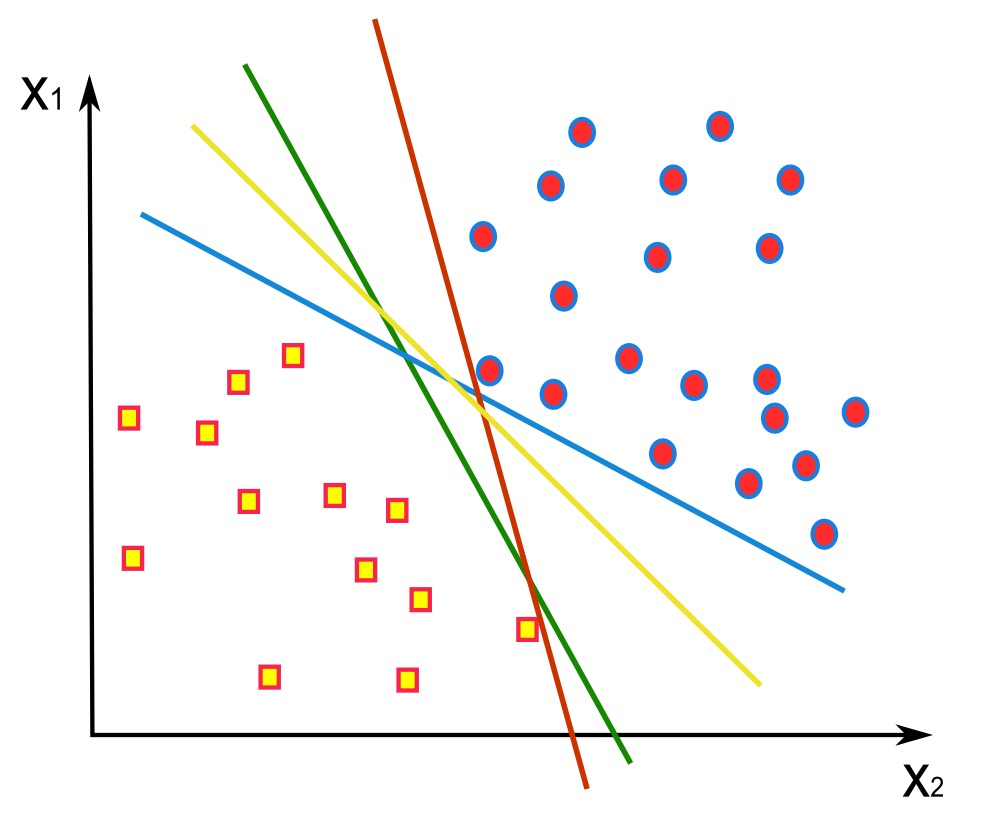
\includegraphics[width=1\textwidth]{2/figures/svm1.jpeg}
		\caption{Hiperplanos de separación(\cite{tecnica3})}
	\end{center}
\end{figure}

\begin{itemize}
	\item \textbf{Margen Geométrico:}
	\begin{itemize}
		\item El margen geométrico se define como:
		\[
		\gamma = \frac{1}{\|w\|}
		\]
		\item El hiperplano de separación óptimo maximiza este margen, mejorando la capacidad de generalización del modelo.
	\end{itemize}
	
	\item \textbf{Optimización del Margen:}
	\begin{itemize}
		\item La optimización del margen geométrico implica minimizar la norma del vector de pesos \( w \).
		\item Esto se resuelve mediante un problema de programación cuadrática para encontrar el hiperplano óptimo y dos hiperplanos paralelos (H1 y H2) que maximicen la distancia entre ellos sin que haya datos entre estos hiperplanos.
	\end{itemize}
	
	\item \textbf{Vectores de Soporte:}
	\begin{itemize}
		\item Los puntos de datos más cercanos al hiperplano de separación, llamados vectores de soporte, definen este hiperplano. Los demás puntos no afectan la solución del SVM.
	\end{itemize}
	
	\item \textbf{Formulación Dual:}
	\begin{itemize}
		\item Se utiliza la formulación dual mediante multiplicadores de Lagrange para simplificar el problema.
		\item Esto permite que los datos de entrenamiento aparezcan solo como productos punto entre vectores, lo cual es fundamental para generalizar el procedimiento a casos no lineales.
		\item La Lagrangiana es:
		\[
		L(w, b, \alpha) = \frac{1}{2} \|w\|^2 - \sum_{i=1}^{l} \alpha_i \left[ y_i \left( w \cdot x_i + b \right) - 1 \right]
		\]
	\end{itemize}
	
	\item \textbf{Solución Dual:}
	\begin{itemize}
		\item La solución del problema dual implica derivar con respecto a \( w \) y \( b \) y luego sustituir estas derivadas en la Lagrangiana original:
		\[
		\frac{\partial L(w, b, \alpha)}{\partial w} = w - \sum_{i=1}^{l} \alpha_i y_i x_i = 0 \Rightarrow w = \sum_{i=1}^{l} \alpha_i y_i x_i
		\]
		\[        \frac{\partial L(w, b, \alpha)}{\partial b} = - \sum_{i=1}^{l} \alpha_i y_i = 0 \Rightarrow \sum_{i=1}^{l} \alpha_i y_i = 0        \]
		\item Los vectores de soporte son aquellos con \( \alpha_i > 0 \), y son cruciales para definir los hiperplanos \( H_1 \) y \( H_2 \).
	\end{itemize}
\end{itemize}
\begin{figure}[H]
	\begin{center}
		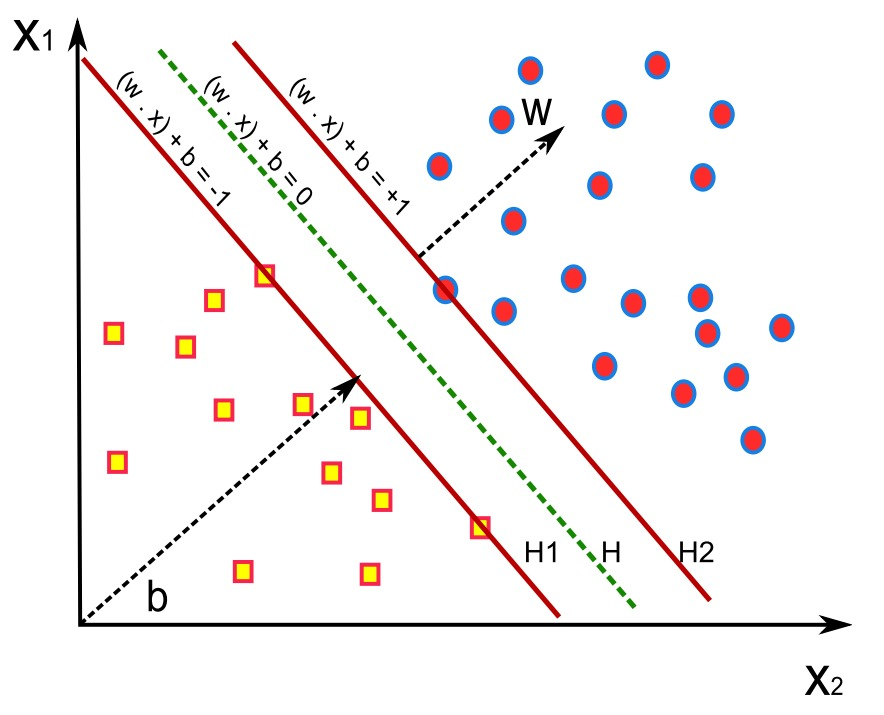
\includegraphics[width=0.8\textwidth]{2/figures/svm2.jpeg}
		\caption{Clasificador óptimo(\cite{tecnica3})}
	\end{center}
\end{figure}

\begin{itemize}
	\item El problema de aprendizaje presentado anteriormente es válido solo para datos linealmente separables, lo cual es raro en la vida real.
	\item En muchos casos, los datos de entrenamiento tienen intersecciones y no pueden ser separados linealmente sin errores.
	\item Los métodos de programación cuadrática anteriores no pueden ser usados en estos casos porque la condición $ y_i ( w \cdot x_i + b ) \geq 1 $ no puede ser satisfecha para todos los puntos de datos.
	\item En casos de intersección, algunos puntos de datos no pueden ser clasificados correctamente, y los valores correspondientes de $ \alpha_i $ tienden a infinito.
	\item Para manejar esto, se introduce el concepto de "soft margin", permitiendo una cierta cantidad de errores de clasificación.
	\item Se agregan variables de holgura no negativas $ \xi_i $ (slack variables) en la ecuación de separación:
	\[
	y_i ( w \cdot x_i + b ) \geq 1 - \xi_i \quad \text{con} \quad \xi_i \geq 0
	\]
\end{itemize}
\begin{figure}[H]
	\begin{center}
		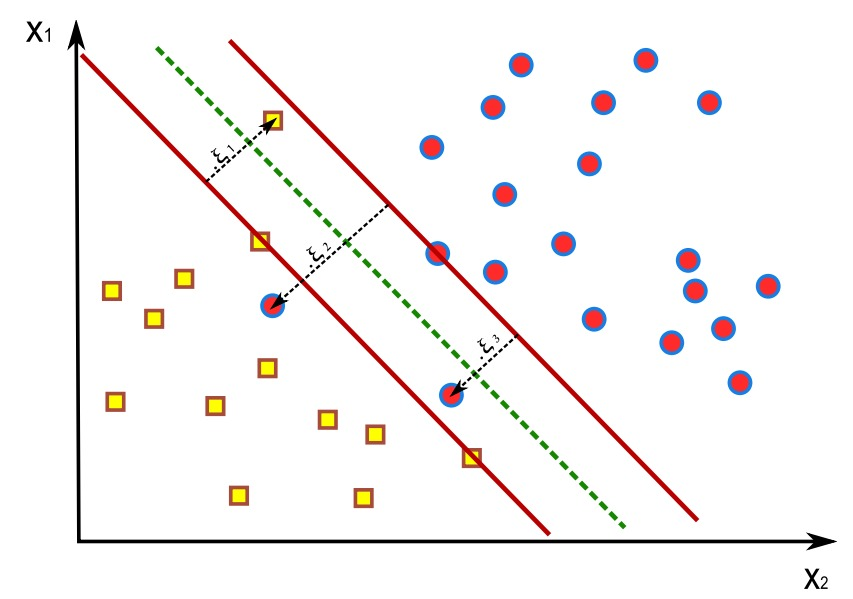
\includegraphics[width=0.8\textwidth]{2/figures/svm3.jpeg}
		\caption{Hiperplanos de margen suave.(\cite{tecnica3})}
	\end{center}
\end{figure}

\begin{figure}[H]
	\begin{center}
		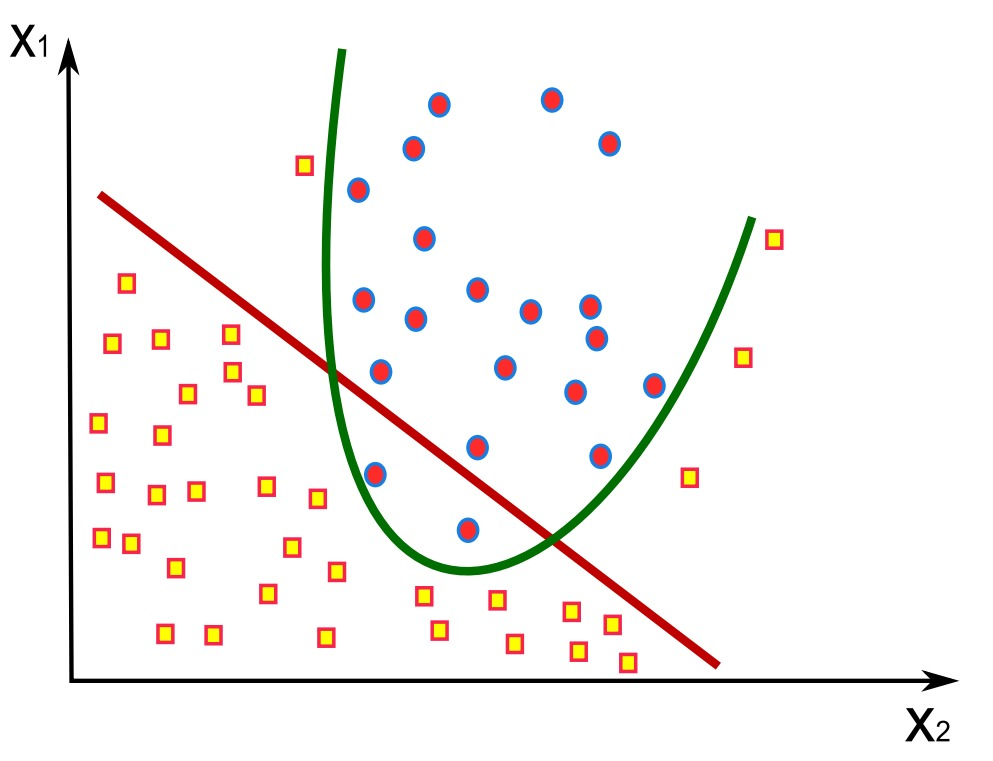
\includegraphics[width=0.8\textwidth]{2/figures/svm4.jpeg}
		\caption{Clasificacion no lineal.(\cite{tecnica3})}
	\end{center}
\end{figure}

En un SVM, el hiperplano óptimo se determina para maximizar la capacidad de generalización del modelo. Sin embargo, si la data de preparacion son linealmente unibles, el clasificador que se tuvo podria no tener una alta capacidad de generalización, incluso si los hiperplanos se determinan de manera óptima. Es decir, para engrandezer el hueco entre clases, el espacio de entrada original se transforma en un espacio de características altamente dimensional llamado ``espacio de características''.

La idea simple en la arquitectura de SVM no lineales es convertir los vectores que recben $x \in \mathbb{R}^n$ en vectores $U(x)$ de un cardumen de características altisimamente dimensional $F$ (donde $U$ representa la asignación: $\mathbb{R}^n \rightarrow \mathbb{R}^f$) y terminar la dificultad de clasificación lineal en este espacio de características. El conjunto de hipótesis consideradas será de la forma:

\[
f(x) = \sum_{i=1}^{l} w_i \phi_i(x) + b
\]

donde $\phi: X \rightarrow F$ es una asignación no lineal de un espacio de entrada a un espacio de características.

Una caracteristica de los componentes de aprendizaje lineales es que pueden expresarse en una vista dual, lo que significa que la ecuación anterior se puede expresar como una combinación lineal de los puntos de datos de entrenamiento. Por lo tanto, la regla de decisión puede evaluarse utilizando productos punto:

\[
f(x) = \sum_{i=1}^{l} \alpha_i y_i K(x_i, x) + b
\]

donde $K(x_i, x)$ es una función kernel que representa el producto punto en el espacio de características.

Los kernel son funciones que satisfacen ciertas propiedades y permiten calcular eficientemente la función de decisión. Algunos de los kernel más utilizados son:

\begin{itemize}
	\item Kernel lineal: $K(x_i, x_j) = (x_i \cdot x_j)$
	\item Kernel Gaussiano: $K(x_i, x_j) = e^{-\frac{||x_i - x_j||^2}{2\sigma^2}}$
	\item Kernel RBF: $K(x_i, x_j) = e^{-c||x_i - x_j||^2}$
	\item Kernel sigmoide: $K(x_i, x_j) = \tanh(g(x_i \cdot x_j) + m)$
\end{itemize}

La elección del kernel depende de las características de los datos y es necesario determinar los parámetros óptimos del kernel utilizado para obtener buenos resultados.

\subsubsection{Debilidades de SVM}
A pesar de la capacidad de generalización y las muchas ventajas de SVM, tienen algunas debilidades muy marcadas, entre las que se encuentran: la selección de parámetros, la complejidad algorítmica que afecta el tiempo de entrenamiento del clasificador en conjuntos de datos grandes, el desarrollo de clasificadores óptimos para problemas multiclase y el rendimiento de SVM en conjuntos de datos desequilibrados.

\paragraph{Complejidad algorítmica}

Limitación principal: alto costo computacional en conjuntos de datos voluminosos. Las SVM, si bien son herramientas poderosas, presentan una desventaja significativa: su elevado costo computacional al trabajar con conjuntos de datos de gran tamaño. La razón de esto reside en el crecimiento cuadrático de la matriz del kernel de entrenamiento con respecto al tamaño del conjunto de datos. Esta dependencia cuadrática deriva en un proceso de entrenamiento sumamente lento para conjuntos de datos voluminosos.

Los métodos de entrenamiento para SVM se pueden categorizar en selección de datos, descomposición, implementaciones geométricas, implementaciones paralelas y heurísticas. Sus ideas centrales y los algoritmos más representativos se presentan en esta sección.

\textbf{Métodos de selección de datos para SVM:} intentan disminuir el tamaño de los conjuntos de datos eliminando las instancias que no contribuyen a la definición del hiperplano separador óptimo. Estos métodos se basan en las instancias que están más cerca del límite de separación y se denominan vectores de soporte (SVs).

\textbf{Métodos de descomposición:} se basan en que el tiempo de entrenamiento se puede reducir si solo se tienen en cuenta las restricciones activas del problema QP. Un método similar a los métodos de conjunto activo para la optimización se aplica en estos métodos de descomposición.

\textbf{Métodos de implementación paralela:} dividen el conjunto de entrenamiento en subconjuntos independientes para entrenar SVM en diferentes procesadores.

\textbf{Métodos geométricos:} están basados en que calcular el hiperplano separador óptimo es equivalente a encontrar el par de puntos más cercanos que pertenecen a envolventes convexas.

\textbf{Métodos heurísticos:} incluyen técnicas como la inicialización de valores de parámetros para el inicio del problema QP, entre otros.



\subsubsection{Implementaciones de SVM}
\paragraph{Resumen de Implementaciones SVM:}
\begin{itemize}
	\item Actualmente existen varias implementaciones de Máquinas de Vectores de Soporte (SVM) en la literatura.
	\item El tiempo computacional varía entre las implementaciones debido a diferentes heurísticas utilizadas para resolver el problema de programación cuadrática.
	\item En conjuntos de datos grandes, las SVM enfrentan tiempos de entrenamiento enormes debido a su complejidad computacional casi cúbica.
\end{itemize}

\paragraph*{Enfoques para Mejorar el Tiempo de Entrenamiento de SVM:}
\begin{itemize}
	\item \textbf{Reducción de Datos:} Se centra en entrenar SVM con un subconjunto de datos probablemente vectores de soporte.
	\item \textbf{Fragmentación (Chunking):} Divide el problema en fragmentos más pequeños, resolviendo cada uno de forma iterativa.
	\item \textbf{Descomposición:} Resuelve una secuencia de problemas de optimización más pequeños para reducir la complejidad.
	\item \textbf{Optimización Secuencial Mínima (SMO):} Optimiza un subconjunto mínimo de dos puntos en cada iteración, escalando bien con conjuntos de datos grandes.
	\item \textbf{Reducción (Shrinking):} Acelera la optimización al reducir el número de valores del kernel necesarios.
	\item \textbf{Selección de Trabajo (Working Selection):} Selecciona un conjunto inicial de variables para optimizar SMO de manera eficiente.
\end{itemize}

\paragraph*{Beneficios de las Implementaciones SVM:}
\begin{enumerate}
	\item Pueden manejar conjuntos de datos grandes de manera eficiente.
	\item Soportan funciones de kernel estándar y personalizadas.
	\item Eficientes para clasificación multiclase y validación cruzada.
	\item Pueden manejar SVM ponderadas para datos desbalanceados.
	\item Proporcionan estimaciones de probabilidad.
\end{enumerate}

\paragraph*{Implementaciones SVM Populares:}
\begin{itemize}
	\item \textbf{SVMLight:} Utiliza técnicas de Selección de Trabajo y Reducción, eficiente para conjuntos de datos grandes.
	\item \textbf{SVMTorch:} Utiliza Selección de Trabajo y Reducción para problemas de regresión a gran escala.
	\item \textbf{Pegasos:} Implementa métodos de descomposición para reducción del tiempo de entrenamiento, adecuado para SVM no lineales.
	\item \textbf{LIBSVM:} Basado en SMO con algoritmo avanzado de selección de conjunto de trabajo, eficiente para conjuntos de datos grandes.
	\item \textbf{SVM Incremental:} Marco para aprendizaje incremental y adaptación de clasificadores SVM.
\end{itemize}

\begin{table}[H]
	\centering
	\caption{Implementaciones SVM}
	\label{tab:svm-implementations}
	\begin{tabular}{p{3cm}p{5cm}p{7cm}}
		\toprule
		\textbf{Implementación} & \textbf{Desarrollador} & \textbf{Código Fuente y Universidad} \\
		\midrule
		SVMTorch & Ronan Collobert and Samy Bengio & C++ - Université de Montréal \\
		Pegasos & Shai Shalev-Shwartz & C++ - The Hebrew University of Jerusalem\\
		LibSVM & Chih-Chung Chang and Chih-Jen Lin & C and Java - National Taiwan University \\
		SVMLight & Thorsten Joachims & C - Cornell University \\
		Incremental SVM & Chris Diehl & M - Carnegie Mellon \\
		\bottomrule
	\end{tabular}
\end{table}

\subsubsection{Aplicaciones en problemas del mundo real en Clasificacion de imagenes}
\paragraph{Clasificación de Cálculos Renales:} En \cite{svmm1}, se emplean filtros de mediana y Gaussiano, y se aplica un enmascaramiento no agudo para mejorar las imágenes. Se utilizan operaciones morfológicas y segmentación basada en entropía para encontrar la región de interés, y luego se emplean técnicas de clasificación KNN y SVM para el análisis de imágenes de cálculos renales.

\paragraph{Detección Temprana de Melanoma:} En \cite{svmm2}, se presenta un dispositivo de manejo con bajo costo y alto rendimiento para mejorar la detección temprana de melanoma en atención primaria. Se propone un sistema de hardware dinámico para implementar un clasificador SVM en cascada en FPGA para la detección temprana de melanoma.

\paragraph{Reconocimiento de Expresiones Faciales:} En \cite{svmm3}, se presenta un marco para el reconocimiento de expresiones independiente de la persona mediante el aprendizaje de múltiples tipos de características faciales a través del aprendizaje de múltiples núcleos en SVM multiclase.

\paragraph{Reconocimiento de Gestos de Mano:} Se aborda el reconocimiento de signos indios basado en técnicas de reconocimiento de gestos de mano dinámicos en escenarios en tiempo real. Se utilizan momentos de Hu y trayectorias de movimiento para la extracción de características y la clasificación de gestos mediante SVM.

\paragraph{Clasificación de Imágenes Hiperespectrales:} En \cite{svmm4}, se propone una técnica para la clasificación espectral-espacial de imágenes hiperespectrales que combina la clasificación pixel a pixel con SVM y la información contextual espacial con un enfoque de Campo Aleatorio de Markov para refinar los resultados de la clasificación.

\paragraph{Selección de Características para la Clasificación de Masas Mammográficas:} En \cite{svmm5}, se abordan métodos de selección de características para la clasificación de masas en mamografías, integrando un procedimiento basado en eliminación recursiva de características SVM con una selección de características de información mutua normalizada.

\paragraph{Clasificación de Imágenes mediante SVM con Kernel de Intersección de Histogramas:} En \cite{svmm6}, se propone un método para la clasificación de imágenes mediante SVM con kernel de intersección de histogramas. Se presenta un solver de kernel de intersección de histogramas determinista y escalable.

\paragraph{Decodificación de Códigos QR a Color:} En \cite{svmm7}, se proponen dos enfoques para resolver problemas de decodificación de códigos QR a color. LSVM-CMI y QDA-CMI, que modelan conjuntamente diferentes tipos de distorsión cromática.


\begin{figure}[H]
	\begin{center}
		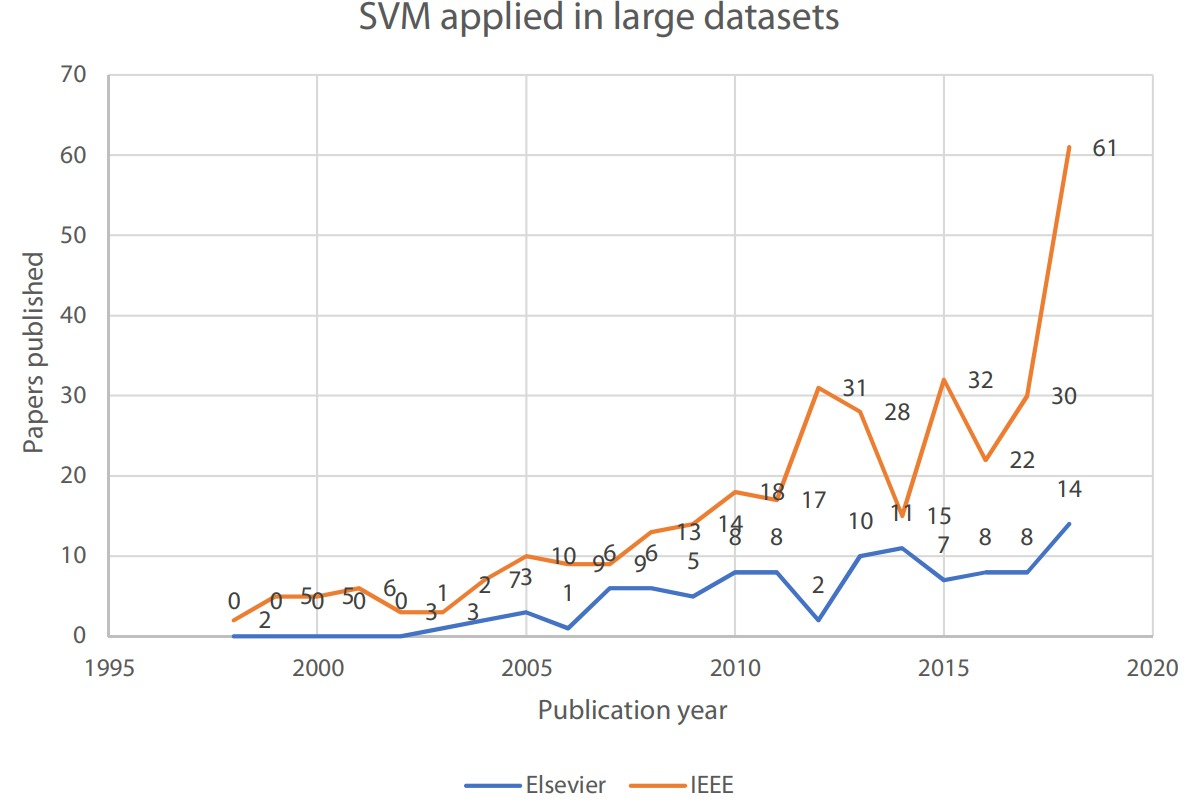
\includegraphics[width=1\textwidth]{2/figures/svm5.jpeg}
		\caption{Número de publicaciones, en capítulos de libros y revistas, por año que contienen los términos de búsqueda SVM y Grandes conjuntos de datos.(\cite{tecnica3})}
	\end{center}
\end{figure}

\begin{figure}[H]
	\begin{center}
		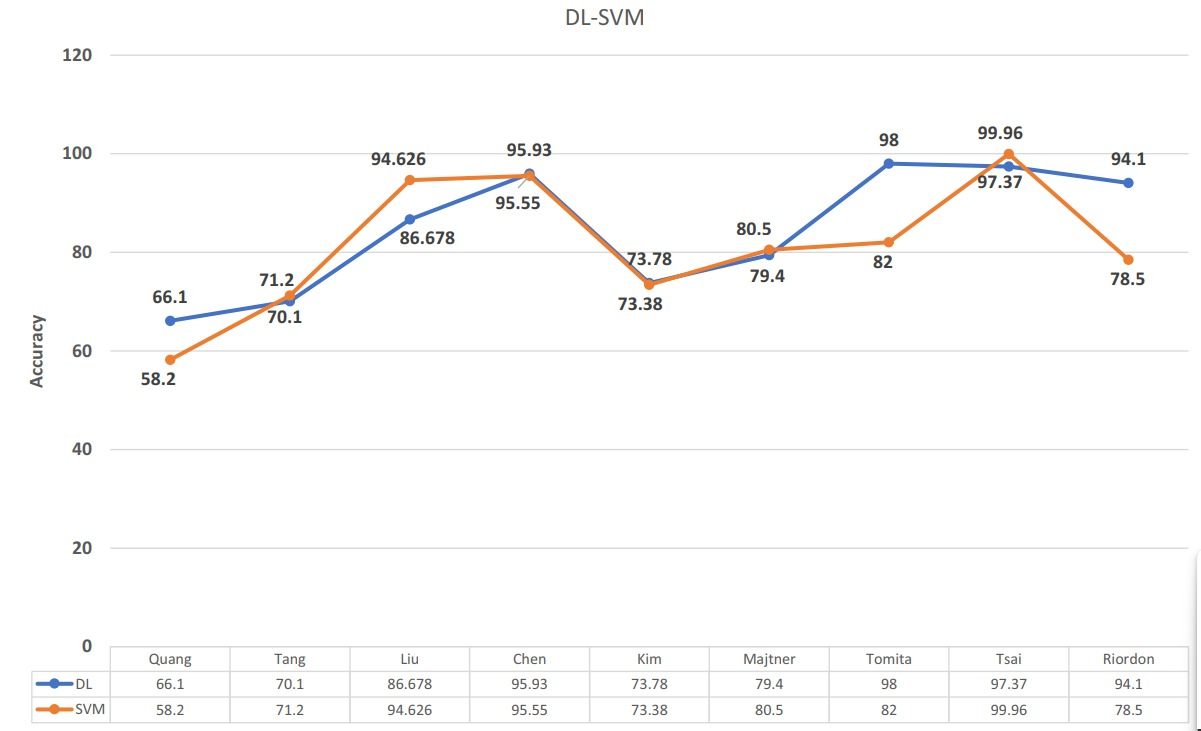
\includegraphics[width=1\textwidth]{2/figures/svm6.jpeg}
		\caption{Rendimiento de SVM frente a Aprendizaje profundo(\cite{tecnica3})}
	\end{center}
\end{figure}

\subsubsection{Conclusiones}
Debido a sus sólidos fundamentos teóricos y capacidad de generalización, entre otras ventajas, las SVM han sido implementadas en muchas aplicaciones del mundo real. Los algoritmos SVM han sido implementados en diversos campos de investigación como: categorización de texto (e hipertexto), detección de pliegues de proteínas y homología remota, clasificación de imágenes, bioinformática (clasificación de proteínas y cáncer), reconocimiento de caracteres escritos a mano, detección de rostros, control predictivo generalizado y muchos más. Muchos investigadores han demostrado que las SVM son mejores que otras técnicas de clasificación actuales. Sin embargo, a pesar de que las SVM tienen algunas limitaciones relacionadas con la selección de parámetros, la complejidad algorítmica, conjuntos de datos multiclase y conjuntos de datos desequilibrados, han sido implementadas en muchos problemas de clasificación de la vida real debido a sus buenos fundamentos teóricos y rendimiento de generalización.

Es importante mencionar que las SVM no son tan populares cuando los conjuntos de datos son muy grandes porque algunas implementaciones de SVM requieren un tiempo de entrenamiento enorme o, en otros casos, cuando los conjuntos de datos están desequilibrados, la precisión de las SVM es pobre. Hemos presentado algunas técnicas para enfrentar estos desequilibrios en los conjuntos de datos. Este artículo describe detalladamente las principales desventajas de las SVM y muchos algoritmos implementados para enfrentar estas desventajas, y cita los trabajos de investigadores que han enfrentado estas desventajas.
\subsection{Redes neuronales convolucionales: Review of Image Classification Algorithms Based on Convolutional Neural Networks \citep*{tecnica2}}
Este artículo destaca el papel crucial de las redes neuronales convolucionales (CNN) en la clasificación de imágenes desde 2012. Explora su evolución desde modelos básicos hasta arquitecturas avanzadas y su influencia en áreas de reconocimiento visual. Compara métodos de clasificación y analiza el impacto de CNN en diversas aplicaciones, subrayando tendencias actuales en el campo. La introducción aborda la importancia de la clasificación de imágenes y su evolución desde la extracción manual de características hasta el uso de CNN, inspiradas en la biología. Modelos como LeNet-5, AlexNet y ZFNet han mejorado significativamente el rendimiento en este ámbito.

A pesar de que las CNN se diseñaron originalmente para la visión por computadora, su aplicación exitosa en el análisis de imágenes de teledetección ha llevado a la necesidad de un análisis sistemático de los métodos de clasificación de imágenes basados en CNN. Este artículo se dedica a detallar el desarrollo de casi todas las arquitecturas de CNN típicas en tareas de clasificación de imágenes, con el objetivo de proporcionar inspiración para el diseño de modelos CNN en el campo del análisis de imágenes de teledetección.


\subsubsection{Visión general de las CNN}
La CNN tiene una estructura principal compuesta por capas convolucionales, de agrupación, de activación no lineal y completamente conectadas. Después de preprocesar la imagen, se introduce en la red a través de la capa de entrada, se procesa mediante capas convolucionales y de agrupación alternadas, y finalmente se clasifica mediante la capa completamente conectada. En comparación con MLP, la CNN agrega capas convolucionales y de agrupación, lo que mejora el rendimiento en términos de tamaño del modelo y capacidad de procesamiento. La capa convolucional identifica eficazmente la correlación entre las características de los píxeles de la imagen, mientras que la capa de agrupación reduce la carga computacional y la sensibilidad excesiva a la posición. La CNN asegura cierto grado de invarianza ante cambios en la imagen como desplazamientos, escalados y distorsiones.

Para CNNs con una cierta profundidad, la operación de convolución de múltiples capas convolucionales puede extraer diferentes características de la entrada. La capa convolucional inferior generalmente extrae características comunes como textura, líneas y bordes, mientras que la capa superior extrae características más abstractas. La capa convolucional tiene varios núcleos de convolución con parámetros aprendibles, que son matrices compuestas por pesos aprendibles. Estas matrices de pesos suelen ser de tamaño 3 × 3, 5 × 5 y 7 × 7, con una longitud y ancho iguales y un número impar. Normalmente, la capa convolucional ingresará a los mapas de características. La matriz de pesos del núcleo de convolución corresponde al área local del mapa de características de conexión, y el núcleo de convolución realiza operaciones de convolución secuenciales en el área del mapa de características mediante deslizamiento. 

La fórmula para la salida de una superficie de características en la capa convolucional puede expresarse aproximadamente como:

\[ \text{{feature\_surface\_out}} = \sum_{i=1}^{N} M_i * W_i + B \]

Donde \( M_i \) representa una superficie de características de los mapas de características de entrada, \( W_i \) es la matriz de pesos del núcleo de convolución, la matriz de sesgo es \( B \), \( f(\cdot) \) es la función de activación no lineal y \( \text{{feature\_surface\_out}} \) es una superficie de características de salida.


\begin{figure}[H]
	\begin{center}
		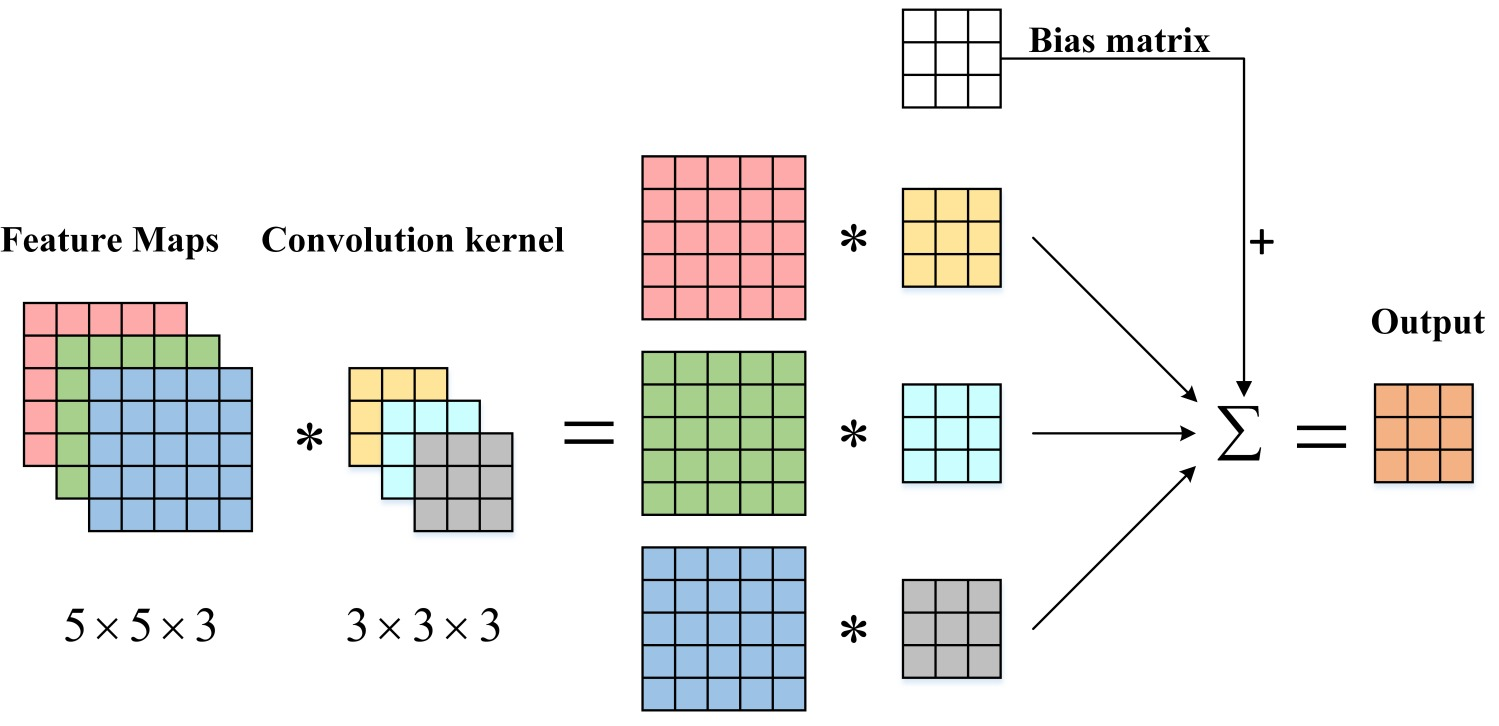
\includegraphics[width=1\textwidth]{2/figures/cnn1.jpeg}
		\caption{Diagrama esquemático del proceso de convolución(\cite{tecnica2})}
	\end{center}
\end{figure}

La capa de agrupación generalmente sigue a la capa convolucional. Las principales razones para usar la capa de agrupación son: realizar un procesamiento de submuestreo y reducción de dimensionalidad en la imagen de entrada para reducir el número de conexiones de la capa convolucional, reduciendo así la carga computacional de la red; lograr invariancia de escala, invariancia de traslación e invariancia de rotación de la imagen de entrada; hacer que el mapa de características de salida sea más robusto ante la distorsión y el error de una sola neurona.

Los métodos de agrupación más utilizados son el promedio y el máximo. Aunque existen otras formas de agrupación que pueden mitigar de manera más efectiva el sobreajuste de las redes neuronales convolucionales, como la Agrupación Lp, Agrupación Mixta, Agrupación Estocástica, Agrupación de Pirámide Espacial (SPP) y Agrupación Ordenada Multiescala, entre otros. Sin embargo, para el modelo clásico de red neuronal convolucional, aunque la mejor operación de agrupación no es la agrupación promedio o la agrupación máxima, son los dos métodos más clásicos. En [72], Bourbeau realizó principalmente un análisis teórico sobre el rendimiento de la agrupación promedio y la agrupación máxima. La operación de agrupación satisface la siguiente relación general entre el tamaño de las matrices de entrada y salida:

\[o = \left( \frac{{i - k}}{s} \right) + 1 \]

\begin{figure}[H]
	\begin{center}
		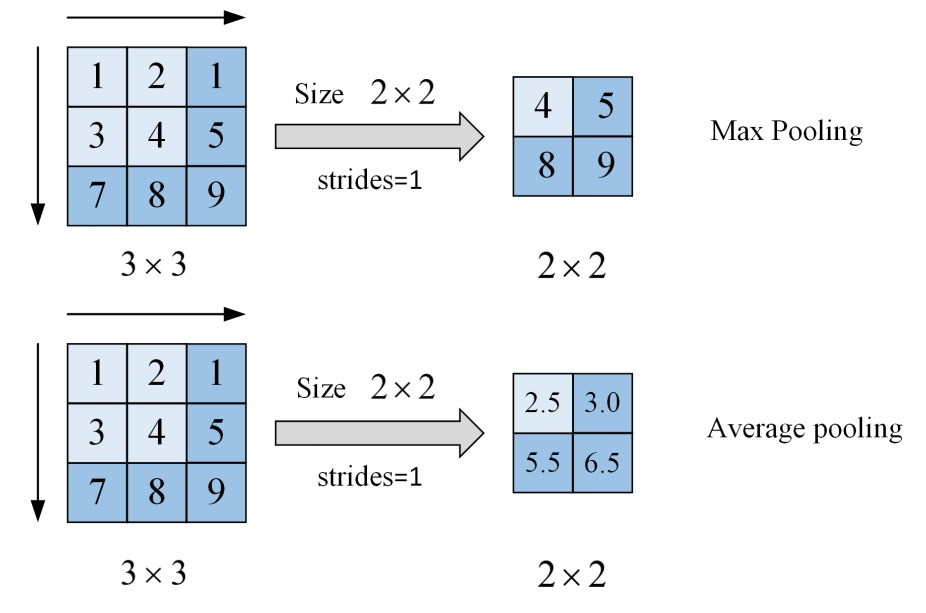
\includegraphics[width=1\textwidth]{2/figures/cnn2.jpeg}
		\caption{Agrupación máxima y agrupación promedio, no implica relleno cero.(\cite{tecnica2})}
	\end{center}
\end{figure}

El propósito de la función de activación es establecer una relación funcional entre la entrada y la salida, introduciendo así un componente no lineal en la red neural. Una función de activación adecuada puede mejorar significativamente el rendimiento de la red. Algunas funciones comunes incluyen sigmoides y Tanh, que son no linealidades saturantes. Sin embargo, para abordar los problemas asociados con estas no linealidades saturantes, se han propuesto funciones no saturantes como ReLU, Leaky ReLU, PReLU, RReLU y ELU. Estas funciones no saturantes son mucho más rápidas para el entrenamiento por descenso de gradiente, lo que resulta en redes mucho más eficientes. Las neuronas con funciones no saturantes se conocen como Unidades Lineales Rectificadas (ReLUs).

En la arquitectura de las CNN, la clasificación final se logra desde la capa de salida, generalmente la última capa de la capa completamente conectada (FC layer). Las diferentes funciones de pérdida también afectan el rendimiento de la arquitectura de la CNN y se aplican a diferentes tareas visuales (como la clasificación de imágenes, reconocimiento facial y reconocimiento de objetos). La función de pérdida más comúnmente utilizada es Softmax+Entropía Cruzada, con muchas versiones mejoradas basadas en ella, como center-loss, L-Softmax, A-Softmax, AM-Softmax, PEDCC-loss, entre otras, que desempeñan un papel importante en diferentes tareas visuales.

\begin{table}[H]
	\centering
	\caption{Funciones de pérdida comunes para modelos CNN.}
	\label{tab:loss_functions}
	\begin{tabular}{p{3cm}p{5cm}p{7cm}}
		\toprule
		Función de Pérdida & Ecuación & Característica \\
		\bottomrule
		L1 (MAE) & $\text{Pérdida}(y, y^*) = \frac{1}{m} \sum_{i=1}^{m} |y^*_i - y_i|$ & Ampliamente utilizado en problemas de regresión. La pérdida L1 se denomina error absoluto medio (MAE). \\
		\midrule
		L2 (MSE) & $\text{Pérdida}(y, y^*) = \frac{1}{m} \sum_{i=1}^{m} (y^*_i - y_i)^2$ & Ampliamente utilizado en problemas de regresión. La pérdida L2 se denomina error cuadrático medio (MSE). \\
		\midrule
		Softmax + Entropía Cruzada & $\text{Pérdida}(y, y^*) = - \sum_{i} y_i \log\left(\frac{\sum_{m}^{i=1} y_i}{\sum_{i}^{m} y_i}\right)$ & Esta función suele emplearse como sustitución del MSE en problemas de clasificación multi-clase. También se utiliza comúnmente en modelos CNN. \\
		\midrule
	\end{tabular}
\end{table}


El flujo de datos en la arquitectura CNN se introduce básicamente en la sección anterior. Entendemos claramente que el entrenamiento de la red se basa en el paso fundamental de la actualización del gradiente, es decir, necesita calcular el gradiente de la función objetivo (función de pérdida) aplicando una derivada de primer orden con respecto a los parámetros de la red, y luego la información del gradiente se transfiere a la capa de red anterior en forma de cálculo de derivada parcial para lograr la actualización de los parámetros de aprendizaje de cada capa de red. La función del optimizador es proporcionar una manera de hacer que la actualización del gradiente sea más razonable, es decir, la macroscópica es que toda la red puede converger más rápido, un valor óptimo local más pequeño (pérdida más pequeña), cálculos más baratos, etc.

\begin{table}[H]
	\centering
	\caption{Métodos de optimización para modelos CNN.}
	\label{tab:optimization_methods}
	\begin{tabular}{p{2.5cm}p{5cm}p{7cm}}
		\toprule
		Nombre & Método & Características \\
		\midrule
		Batch Gradient Descent (BGD) & Calcula el gradiente de todo el conjunto de entrenamiento y posteriormente utiliza este gradiente para actualizar los parámetros. & 1. Para un conjunto de datos de pequeño tamaño, el modelo CNN converge más rápido y crea un gradiente extra estable utilizando BGD. 2. Generalmente no es adecuado para un conjunto de entrenamiento grande. 3. Requiere una cantidad sustancial de recursos. \\
		\midrule
		Stochastic Gradient Descent (SGD) & Muestrea seleccionando arbitrariamente parte del conjunto de entrenamiento. & 1. Para un conjunto de entrenamiento de gran tamaño, esta técnica es más eficiente en memoria y mucho más rápida que BGD. 2. Se introduce aleatoriedad y ruido debido a sus actualizaciones frecuentes. Su convergencia no es estable, pero la expectativa sigue siendo igual al descenso de gradiente correcto. \\
		\midrule
		Mini-batch Gradient Descent & Divide las muestras de entrenamiento en varios mini lotes, y luego se realiza la actualización de parámetros siguiendo el cálculo del gradiente en cada mini lote. & Este método combina las ventajas técnicas de SGD y SGD, que tienen una convergencia estable, más eficiencia computacional y una eficacia de memoria extra. \\
		\midrule
		Momentum & Introduce un parámetro de momento en SGD que acumula información de gradiente histórica. & Cuando el entrenamiento cae en un mínimo local, la información del gradiente con momento puede ayudar a la red a escapar y encontrar el mínimo global. \\
		\midrule
		Adaptive Moment Estimation (Adam) & Calcula una tasa de aprendizaje adaptativa para cada parámetro en el modelo. & Se combinan las ventajas del momento y RMSprop. Es ampliamente utilizado en el aprendizaje profundo y representa la última tendencia de optimización. \\
		\bottomrule
	\end{tabular}
\end{table}
\subsubsection{Clasificación de imágenes basada en CNN}
En general, la clasificación de imágenes implica extraer características de la imagen manualmente o mediante métodos de aprendizaje de características, y luego usar un clasificador para identificar la categoría del objeto. Antes del aprendizaje profundo, se utilizaba ampliamente el modelo de Bag of Words, que involucraba tres procesos: extracción de características de bajo nivel, codificación de características y diseño de clasificador. Este método tradicional fue común hasta 2012, siendo utilizado en competiciones como PASCAL VOC y ILSVRC 2010. Sin embargo, la aparición de las CNNs revolucionó la clasificación de imágenes, permitiendo un aprendizaje de características más eficaz y un proceso de clasificación de extremo a extremo que no requiere la extracción manual de características, superando las limitaciones de los métodos tradicionales. Esta sección presenta los modelos clásicos de clasificación de imágenes basados en CNN a lo largo del tiempo.



\begin{itemize}
	\item \textbf{LeNet Network:} En 1998, Lecun  desarrolló el modelo LeNet-5 para clasificar imágenes digitalmente, superando a otros métodos de la época y utilizando retropropagación por primera vez en CNNs. LeNet-5, con 7 capas y ~60k parámetros, se divide en un área de convolución y un área FC, utilizando la función de activación sigmoid y el clasificador softmax. Aunque tuvo buenos resultados en MNIST, su rendimiento en conjuntos de datos más grandes fue limitado debido a la complejidad computacional y la falta de investigación en inicialización de parámetros y algoritmos de optimización. Eventualmente, fue superado por otros métodos de aprendizaje automático como SVM.
	\item \textbf{AlexNet Network:} En 2012, AlexNet, desarrollado por Krizhevsky et al., ganó la ILSVR 2012 con gran ventaja, demostrando que las características aprendidas superan a las diseñadas manualmente. Utilizó procesamiento paralelo entre GPUs debido a las limitaciones de la GPU GTX 580. AlexNet tiene 8 capas y ~60M parámetros, con 5 capas de convolución y 3 capas FC. Requiere un tamaño de convolución mayor para las imágenes más grandes de ImageNet. Mejoras clave incluyen:
	ReLU: Aceleró la convergencia y redujo la desaparición del gradiente.
	Dropout: Controló la complejidad del modelo y mitigó el sobreajuste.
	Aumento de datos: Usó técnicas como volteo, recorte y cambios de color para ampliar conjuntos de datos y reducir el sobreajuste.
	Pooling superpuesto: Mejoró la precisión del modelo y alivió el sobreajuste.
	
	
	
	\begin{figure}[H]
		\begin{center}
			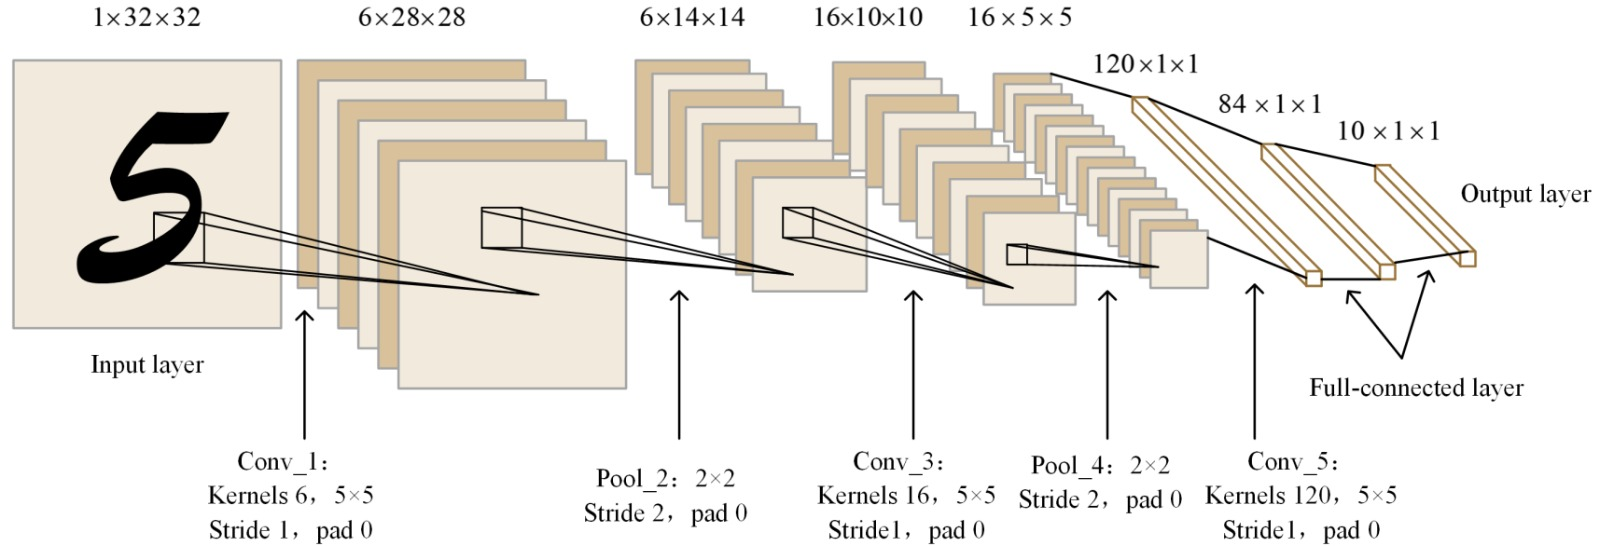
\includegraphics[width=1\textwidth]{2/figures/cnn3.jpeg}
			\caption{La arquitectura de la red LeNet-5. La forma de salida es canal × altura × anchura. Cada capa convolucional
				Utiliza tallas 5 × 5, relleno 0, zancadas 1. Cada capa de agrupación tiene un tamaño de 2 × 2 y zancadas 2.(\cite{tecnica2})}
		\end{center}
	\end{figure}
	\item \textbf{VGGNet:} En 2014, Simonyan et al. propusieron el modelo VGG, obteniendo el segundo lugar en ILSVR 2014. Similar a AlexNet, VGG usa una estructura de área de convolución seguida de área FC. Utiliza varias capas de convolución idénticas seguidas de una capa de pooling que reduce la altura y anchura a la mitad. VGG-16, una variante con 16 capas, conecta cinco bloques en serie y termina con dos capas FC de 4096 neuronas y una capa de salida de 1000 clasificaciones.
	
	Mejoras respecto a AlexNet:
	
	Red modular: Uso de módulos básicos para construir el modelo.
	Convoluciones más pequeñas: Filtros de 3x3 que aumentan la profundidad y reducen parámetros comparado con filtros más grandes.
	Entrenamiento multi-escala: Escala la imagen de entrada y la recorta aleatoriamente, logrando aumento de datos y previniendo el sobreajuste.
	
	\begin{figure}[H]
		\begin{center}
			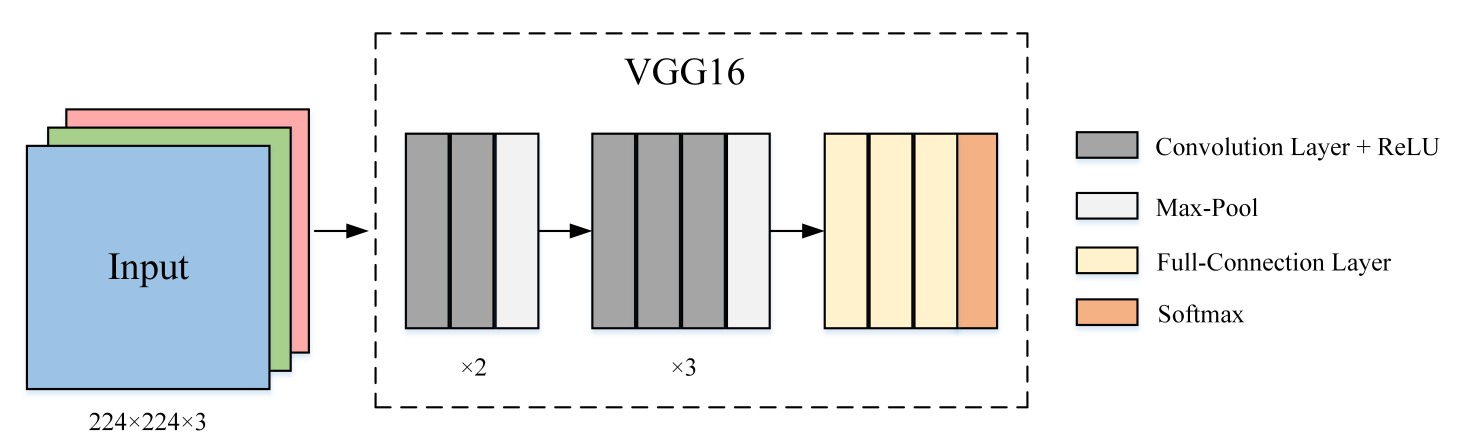
\includegraphics[width=1\textwidth]{2/figures/cnn4.jpeg}
			\caption{ La arquitectura de la red VGG-16. Conv: tamaño = 3 × 3, zancada = 1, relleno = 1. Piscina:
				tamaño = 3 × 3, zancada = 2.
				(\cite{tecnica2})}
		\end{center}
	\end{figure}
	\item \textbf{ GoogLeNet/InceptionV1 to V4:}En 2014, GoogLeNet, propuesta por Christian Szegedy et al., ganó el campeonato de ILSVR 2014 introduciendo el módulo Inception.
	
	InceptionV1:
	
	Tiene 22 capas y alrededor de 6 millones de parámetros.
	El módulo Inception contiene 4 ramas paralelas: tres con capas de convolución de diferentes tamaños (1x1, 3x3, 5x5) y una con una capa de max-pooling, seguido de convolución 1x1.
	Mejora la adaptabilidad y la fusión multi-escala al aumentar el ancho del modelo.
	
	InceptionV2:
	
	Reemplaza convoluciones de 5x5 con dos convoluciones de 3x3 para reducir el tiempo de cálculo.
	Introduce Batch Normalization (BN) para estabilizar y acelerar el entrenamiento mediante la normalización de las entradas de las capas.
	
	InceptionV3:
	
	Utiliza convoluciones factoradas y asimétricas, reemplazando una convolución 3x3 por una 1x3 seguida de una 3x1 para reducir los parámetros y mejorar la eficiencia computacional.
	Implementa reducción del tamaño de la cuadrícula mediante operaciones de pooling y convoluciones con stride 2.
	Introduce técnicas adicionales para optimizar la eficiencia computacional y prevenir el sobreajuste, como el uso de múltiples tamaños de escala para las imágenes de entrada.
	\begin{figure}[H]
		\begin{center}
			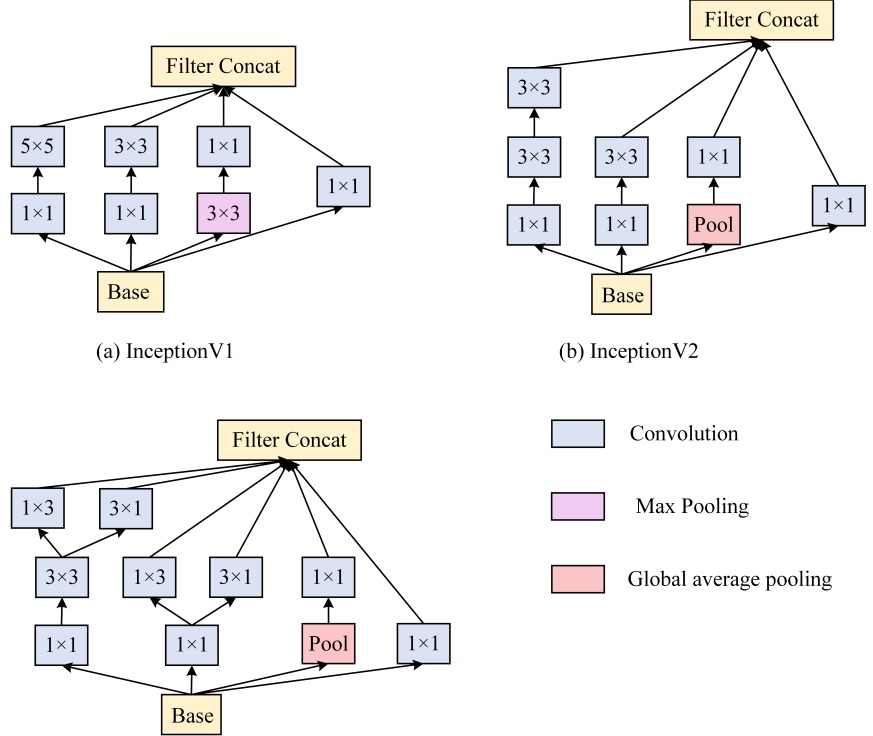
\includegraphics[width=1\textwidth]{2/figures/cn55.jpeg}
			\caption{  Módulo InceptionV1 a V3
				(\cite{tecnica2})}
		\end{center}
	\end{figure}
	InceptionV4:
	
	Reduce la complejidad de InceptionV3 mediante la unificación de las opciones de cada bloque de Inception.Los bloques de Inception y de Reducción son utilizados para simplificar y optimizar la arquitectura. El "stem" de la arquitectura se modifica para ser más uniforme y mejorar la eficiencia. Se optimiza el uso de memoria durante la retropropagación, permitiendo entrenar el modelo sin particionar réplicas.
	
	\begin{figure}[H]
		\begin{center}
			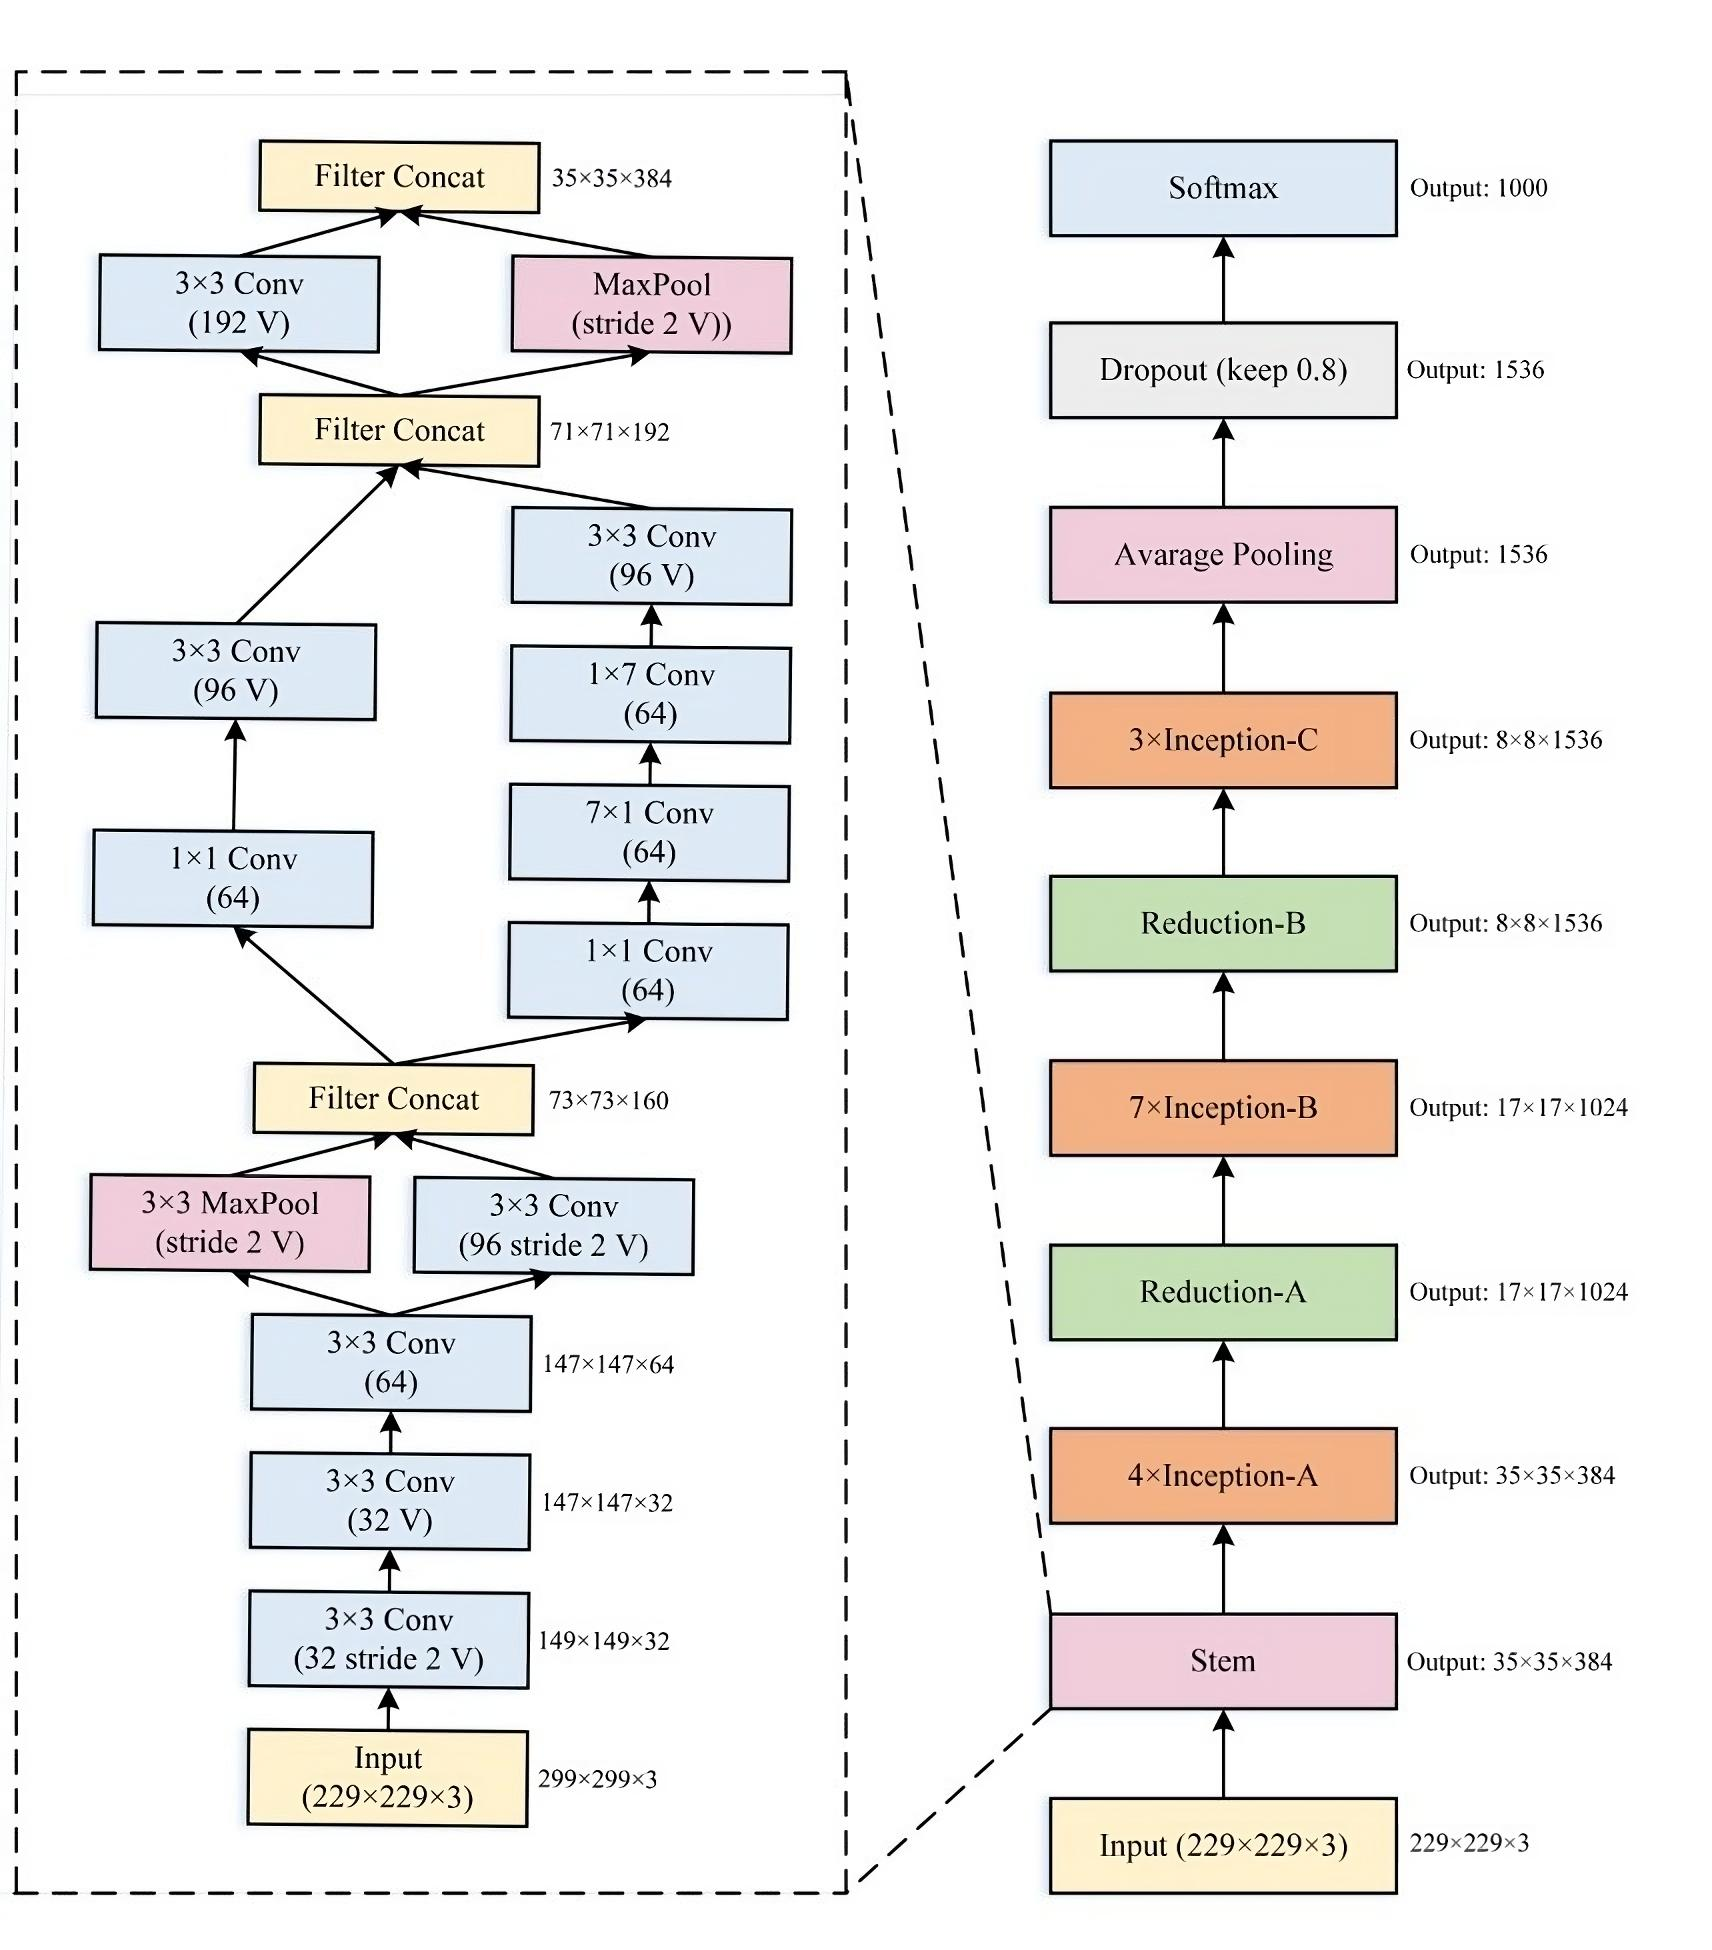
\includegraphics[width=1\textwidth]{2/figures/cnn6.jpeg}
			\caption{ Arquitectura general de InceptionV4. La parte superior de la imagen es la estructura general, la parte inferior de la
				La imagen es el tallo de la arquitectura.
				(\cite{tecnica2})}
		\end{center}
	\end{figure}
	
	\item \textbf{Residual Learning Networks (ResNet):} En 2015, la red residual profunda ResNet, propuesta por Kaiming He et al., ganó el primer premio en ILSVR2015. A medida que las redes se vuelven más profundas, aumenta el rendimiento de la red, pero simplemente aumentar la profundidad de la red no mejora efectivamente el rendimiento. ResNet aborda este problema mediante conexiones residuales, que permiten que las redes profundas alcancen una alta precisión. En lugar de aprender la asignación deseada directamente, las conexiones residuales ajustan una asignación residual relacionada con la identidad, lo que facilita la optimización y el aprendizaje. Los bloques residuales en ResNet contienen dos capas convolucionales 3x3, seguidas de normalización y activación ReLU, con una conexión directa de entrada al bloque final. Para profundidades mayores, se puede añadir una capa convolucional 1x1 para controlar el número de canales. ResNet ha demostrado ser una contribución significativa al lograr precisión incluso con profundidades mayores, superando a las redes previas.En 2015, ResNet, una red residual profunda propuesta por Kaiming He et al., ganó el primer premio en ILSVR2015. A medida que las redes se vuelven más profundas, el rendimiento aumenta, pero simplemente aumentar la profundidad no garantiza una mejora efectiva. ResNet aborda este desafío mediante conexiones residuales, que permiten a las redes profundas alcanzar altos niveles de precisión. En lugar de aprender directamente la asignación deseada, las conexiones residuales ajustan una asignación residual relacionada con la identidad, lo que facilita la optimización y el aprendizaje. Los bloques residuales en ResNet consisten en dos capas convolucionales 3x3, seguidas de normalización y activación ReLU, con una conexión directa de entrada al bloque final. Para profundidades mayores, se puede añadir una capa convolucional 1x1 para controlar el número de canales. ResNet ha demostrado ser una contribución significativa al lograr una alta precisión incluso con profundidades mayores, superando a las redes anteriores.
	
	\item \textbf{Mejoras de ResNet:}
	ResNet con preactivación: He et al. introdujeron una estructura de preactivación que mejora el rendimiento de ResNet al preactivar la BN y ReLU. Este enfoque permite el entrenamiento exitoso de ResNet con más de 1000 capas, enfatizando la importancia del mapeo de identidad.
	
	Profundidad estocástica: El método de profundidad estocástica, propuesto por Huang et al., elimina ciertas capas durante el entrenamiento, reduciendo significativamente el tiempo de entrenamiento y aumentando la profundidad de ResNet. Este método resulta efectivo incluso con más de 1200 capas, mejorando el error de prueba y el tiempo de entrenamiento en los conjuntos de datos CIFAR-10/100.
	
	Redes Residuales Amplias (WRNs): Para contrarrestar la desaceleración del entrenamiento debido a la disminución de la reutilización de características en redes más profundas, las WRNs introducen bloques de eliminación amplia, ampliando las capas de peso de las unidades residuales originales y agregando eliminación entre ellas. Este enfoque, con menos capas que las ResNets más profundas, reduce el tiempo de entrenamiento y tiene un mejor rendimiento en los conjuntos de datos CIFAR e ImageNet.
	
	ResNeXt: ResNeXt introduce el concepto de "Cardinalidad C", el número de rutas en un bloque, para superar los desafíos de adaptación del conjunto de datos. Aumentar la cardinalidad resulta más efectivo que aumentar la profundidad o el ancho. Las estructuras de convolución agrupada, como en la Figura 18c, son más rápidas y eficientes, formando la base de ResNeXt.
	
	Redes Residuales Dilatadas (DRN): Yu et al. abordan la pérdida de resolución y la reducción de la información de características en el submuestreo al introducir convoluciones dilatadas. Estas convoluciones aumentan el campo receptivo de las capas superiores, compensando la reducción de campos receptivos inducida por la eliminación del submuestreo. DRN logra una precisión significativamente mejorada en la clasificación de imágenes en comparación con ResNet.
	
	Otros modelos: Variantes como la ResNet reducida de Veit et al., Resnet en Resnet (RiR), la técnica DropBlock, Big Transfer (BiT) y NFNet, ofrecen enfoques únicos para mejorar el rendimiento de ResNet. Estos métodos incluyen la eliminación de capas, arquitecturas de doble flujo, eliminación de características y estructuras sin BN, logrando mejoras notables en velocidad de entrenamiento y precisión.
	
	\begin{figure}[H]
		\begin{center}
			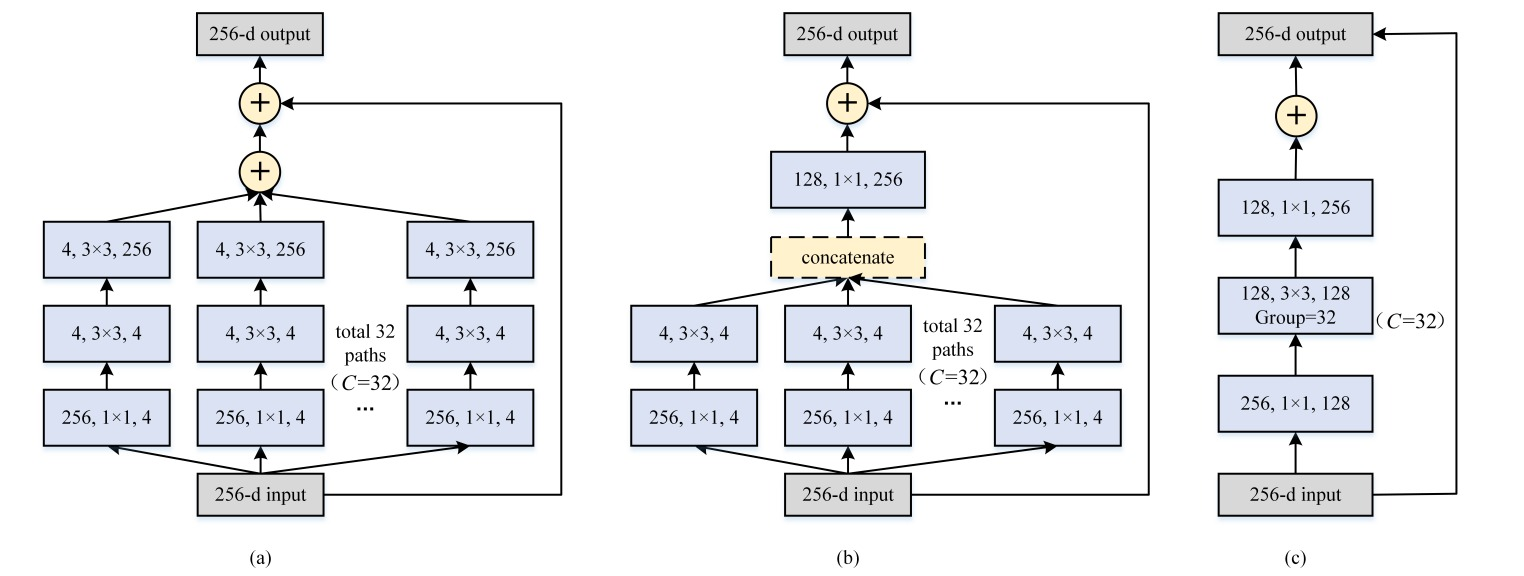
\includegraphics[width=1\textwidth]{2/figures/cnn7.jpeg}
			\caption{Bloques de construcción equivalentes de ResNeXt.
				(\cite{tecnica2})}
		\end{center}
	\end{figure}
	
	\item \textbf{MobileNet V1 to V3:} En 2017, Google presentó MobileNetV1, una red liviana diseñada para dispositivos móviles y embebidos. Utiliza convolución separable en profundidad, que consta de convolución en profundidad y convolución puntual, en lugar de convolución estándar, reduciendo significativamente el costo computacional y los parámetros. MobileNetV1 ofrece dos hiperparámetros, el multiplicador de ancho x y el multiplicador de resolución x, para equilibrar eficazmente el cálculo y la precisión.
	
	En 2018, MobileNetV2 abordó el problema de los parámetros cero en la convolución separable en profundidad al introducir Residuos Invertidos y Cuellos de Botella Lineales. A diferencia del bloque residual estándar, el bloque residual invertido de MobileNetV2 sigue una secuencia de 1 × 1 (expansión) → 3 × 3 → 1 × 1 (compresión). Además, reemplaza el último ReLU con una transformación lineal para evitar la pérdida de información.
	
	En 2019, MobileNetV3 mejoró la eficiencia y precisión al incorporar el bloque SE para atención por canal y la tecnología de Búsqueda de Arquitectura Neural (NAS). El enfoque NAS consciente de la plataforma se utiliza para la búsqueda por bloques para encontrar estructuras globales de red, mientras que NetAdapt ajusta individualmente las capas de manera secuencial. MobileNetV3 también adopta la función de activación h-swish, modificando el sigmoidal de la función swish para mejorar la precisión.
	
	\begin{figure}[H]
		\begin{center}
			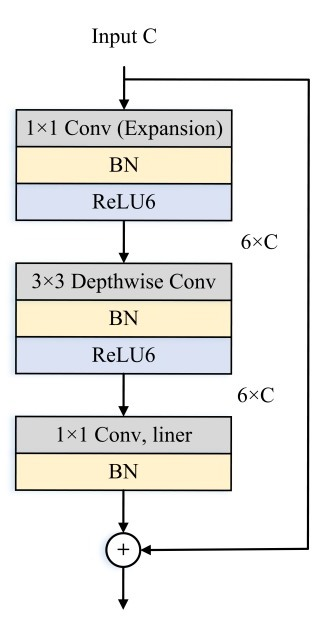
\includegraphics[width=0.6\textwidth]{2/figures/cnn8.jpeg}
			\caption{  El bloque residual de cuello de botella de MobileNetV2. C es el número de canales y las relaciones de expansión son 6.
				(\cite{tecnica2})}
		\end{center}
	\end{figure}
	
	
	\item \textbf{ShuffleNet V1 to V2:}
	
	En 2017, ShuffleNetV1, desarrollado por Face++, se enfocó en plataformas móviles como drones, robots y teléfonos inteligentes. Utiliza convolución Pointwise Group y Channel Shuffle para mejorar el bloque residual. La convolución Pointwise Group resuelve el problema de los canales limitados debido a convoluciones costosas, mientras que Channel Shuffle aborda la pérdida de información entre grupos de canales en bloques de convolución de grupo. La unidad ShuffleNet (stride = 1) reemplaza la primera convolución 1 × 1 con convolución de grupo pointwise seguida de una operación de mezcla de canales. La unidad ShuffleNet (stride = 2) agrega un GAP de 3 × 3 a la ruta de acceso directo y reemplaza la concatenación de canales con una suma de elementos. MobileNetV1 experimentó con diferentes números de grupos para convoluciones y escalas para el número de filtros.
	
	En 2018, ShuffleNetV2 optimizó la velocidad y precisión considerando la complejidad computacional, el costo de acceso a la memoria y las características de la plataforma. Cuatro directrices principales surgieron de los experimentos: el ancho de canal igual minimiza el costo de acceso a la memoria; la convolución de grupo excesiva aumenta este costo; la fragmentación de la red reduce el paralelismo y las operaciones elemento a elemento tienen una alta relación MAC/FLOPs. La unidad ShuffleNetV2 evita violar estas directrices para mejorar la eficiencia.
	\begin{figure}[H]
		\begin{center}
			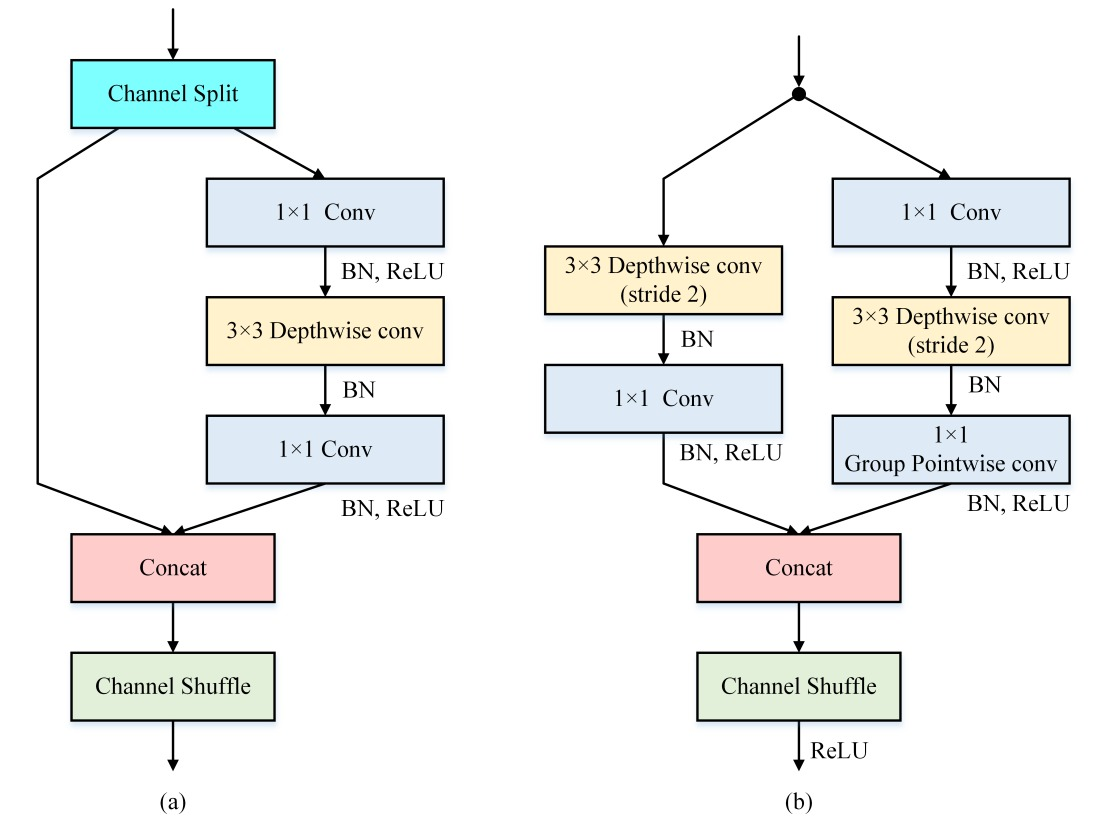
\includegraphics[width=1\textwidth]{2/figures/cnn9.jpeg}
			\caption{  El bloque residual de cuello de botella de MobileNetV2. C es el número de canales y las relaciones de expansión son 6.
				(\cite{tecnica2})}
		\end{center}
	\end{figure}
	
	\item \textbf{Data Augmentation:} as CNN a menudo enfrentan el riesgo de sobreajuste debido a datos limitados. Las técnicas tradicionales de aumento de datos incluyen una colección de métodos, como voltear, cambiar el espacio de color, recortar, rotar, trasladar e inyectar ruido, que pueden mejorar los atributos y el tamaño del conjunto de datos de entrenamiento. Además, tienen el potencial de mejorar significativamente la generalización de los modelos de DL. El aumento de datos automatizado tiene el potencial de abordar algunas debilidades de los métodos tradicionales de aumento de datos, ya que entrenar un modelo CNN con una política de aumento de datos aprendida puede mejorar significativamente la precisión, la robustez del modelo y el rendimiento en el aprendizaje semi-supervisado para la clasificación de imágenes. La técnica de Aumento de Datos de Muestra Mixta (MSDA) consiste en mezclar aleatoriamente dos muestras de entrenamiento y sus etiquetas según una cierta proporción, lo que no solo puede reducir la identificación errónea de algunas muestras difíciles, sino también mejorar la robustez del modelo y hacerlo más estable durante el entrenamiento.
\end{itemize}
\subsubsection{Conclusiones} 
Esta revisión abarca no solo los modelos convencionales de CNN, sino también métodos mixtos y estrategias de entrenamiento, destacando puntos clave en la clasificación de imágenes.

Los modelos clásicos de CNN (2012-2017) sentaron las bases para el diseño estructural actual. La integración del mecanismo de atención en las CNN, como los bloques SE, mejora su rendimiento. Las redes para plataformas móviles son más pequeñas y eficientes, aprovechando al máximo los recursos limitados. La elección de hiperparámetros es crucial, y la búsqueda NAS facilita el diseño de redes de alto rendimiento. El aprendizaje por transferencia y el aumento de datos mejoran las predicciones y el rendimiento.

Los modelos livianos sacrifican precisión por eficiencia, y aún se explora su uso en sistemas limitados. El campo de NLP ha avanzado más en el aprendizaje semi-supervisado y no supervisado.

Futuras direcciones incluyen la combinación de convolución y Transformer, como en la red CoAtNet, y la revisión de componentes convencionales de CNN, que podría llevar a avances significativos.
\subsection{Vision Transformer: Explainability of Vision Transformers: A Comprehensive Review and New Perspectives \citep*{tecnica1}}
Los transformers han sido importantes en el procesamiento del lenguaje y, recientemente, se han destacado en la visión por computadora. Aunque su funcionamiento interno no se comprende completamente, la explicabilidad es crucial. Este estudio revisa métodos de explicabilidad para transformers visuales, propone una taxonomía y ofrece criterios de evaluación y herramientas. También señala áreas no exploradas que podrían mejorar la explicabilidad y sugiere futuras investigaciones.

\subsubsection{Introducción}
La Inteligencia Artificial (IA) ha experimentado avances notables en los últimos años, principalmente impulsada por el éxito de las Redes Neuronales Profundas (DNNs) en una amplia gama de aplicaciones, como el diagnóstico médico, las aplicaciones financieras, las evaluaciones de riesgos y la generación de imágenes y videos. Estos logros han sido significativos en términos de rendimiento y precisión en diversas tareas, sin embargo, la aplicación práctica de las DNNs sigue siendo limitada debido a su naturaleza opaca y la falta de transparencia en su toma de decisiones.

La opacidad de las DNNs plantea preocupaciones importantes en términos de confiabilidad y seguridad, ya que los usuarios y los responsables de la toma de decisiones pueden tener dificultades para comprender por qué un modelo ha llegado a una determinada conclusión o recomendación. Esto es particularmente problemático en áreas donde las decisiones basadas en IA pueden tener un impacto significativo en la vida de las personas, como la salud y la justicia. La falta de transparencia también puede ocultar sesgos y errores en los modelos, lo que socava aún más la confianza en su uso.

Para abordar estos desafíos, ha surgido el campo de la Inteligencia Artificial Explicable (XAI), cuyo objetivo es mejorar la comprensión y la transparencia de los modelos de IA. La XAI busca proporcionar explicaciones claras y comprensibles sobre cómo se toman las decisiones por parte de los modelos de IA, permitiendo a los usuarios entender y confiar en sus resultados. Al comprender cómo funciona un modelo y por qué toma ciertas decisiones, los usuarios pueden evaluar mejor su fiabilidad y corregir posibles sesgos o errores.

En este contexto, los transformers, modelos basados en atención, han surgido como una alternativa poderosa a las arquitecturas de redes neuronales convolucionales (CNNs) tradicionales en áreas como el Procesamiento del Lenguaje Natural (NLP) y la Visión por Computadora (CV). Los transformers han demostrado ser altamente efectivos para capturar relaciones a largo plazo en datos secuenciales, lo que los hace adecuados para tareas que requieren un procesamiento de contexto complejo.

En particular, los Vision Transformers (ViT) aplican la arquitectura de transformers a la tarea de visión por computadora, lo que ha llevado a avances significativos en tareas como el reconocimiento de imágenes, la detección de objetos y la segmentación de imágenes. Los ViT han demostrado resultados comparables e incluso superiores a los obtenidos con CNNs en algunas aplicaciones.

Sin embargo, a pesar de su éxito, la comprensión y la explicabilidad de los transformers, especialmente en el contexto de la visión por computadora, siguen siendo áreas de investigación activa. Se necesitan métodos y técnicas robustas para explicar las decisiones tomadas por estos modelos, así como herramientas y marcos para evaluar y comparar sus explicaciones. Al mejorar la explicabilidad de los transformers, podemos fortalecer la confianza en su uso y abrir nuevas oportunidades para aplicaciones prácticas en una variedad de campos.

\subsubsection{ Arquitectura de Vision Transformer}
Los Vision Transformers (ViTs) aprovechan los avances de los transformers en NLP para aplicaciones visuales. Utilizan bloques de transformers que permiten integrar información global en toda la imagen mediante auto-atención. Las imágenes se representan como secuencias de tokens, con una capa de incrustación de parches para dividirlas en parches. Estos parches se aplanan y se tratan como tokens, luego se transforman en vectores de características. Para la clasificación, se agrega un token de clasificación. La red ViT también incluye otros componentes como una activación GELU, normalización de capa y conexión residual.Se puede encontrar una ilustración de la arquitectura ViT en la Figura 7.
\begin{figure}[H]
	\begin{center}
		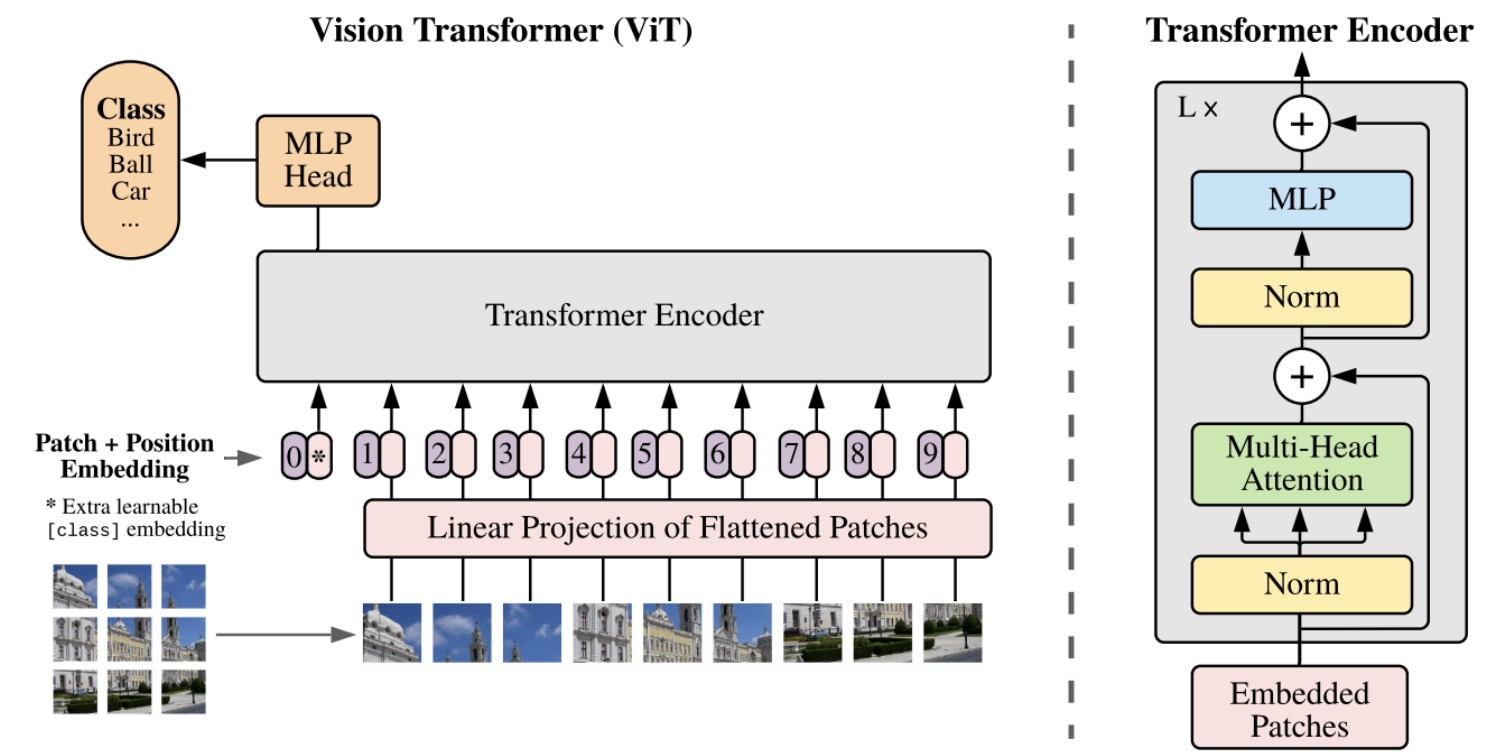
\includegraphics[width=1\textwidth]{2/figures/vt1.jpeg}
		\caption{Arquitectura de Vision Transformer (\cite{tecnica1})}
	\end{center}
\end{figure}

\subsubsection{ Explicacion y métodos para Visual Transformer} 
Tras los trabajos innovadores presentados basados en transformers visuales para diversos dominios de visión por computadora, han surgido múltiples enfoques para mejorar la explicabilidad de estas redes. Sin embargo, se necesita una encuesta exhaustiva para comprender mejor estos métodos e identificar áreas de mejora. Con un enfoque en la tarea de clasificación, esta sección presenta una visión general de las técnicas de explicabilidad existentes para transformers visuales. Para proporcionar una visión clara, categorizamos y resumimos estos métodos en cinco grupos distintos según sus procedimientos de trabajo, motivaciones y características estructurales, como se ilustra en la Figura 8.
\begin{figure}[H]
	\begin{center}
		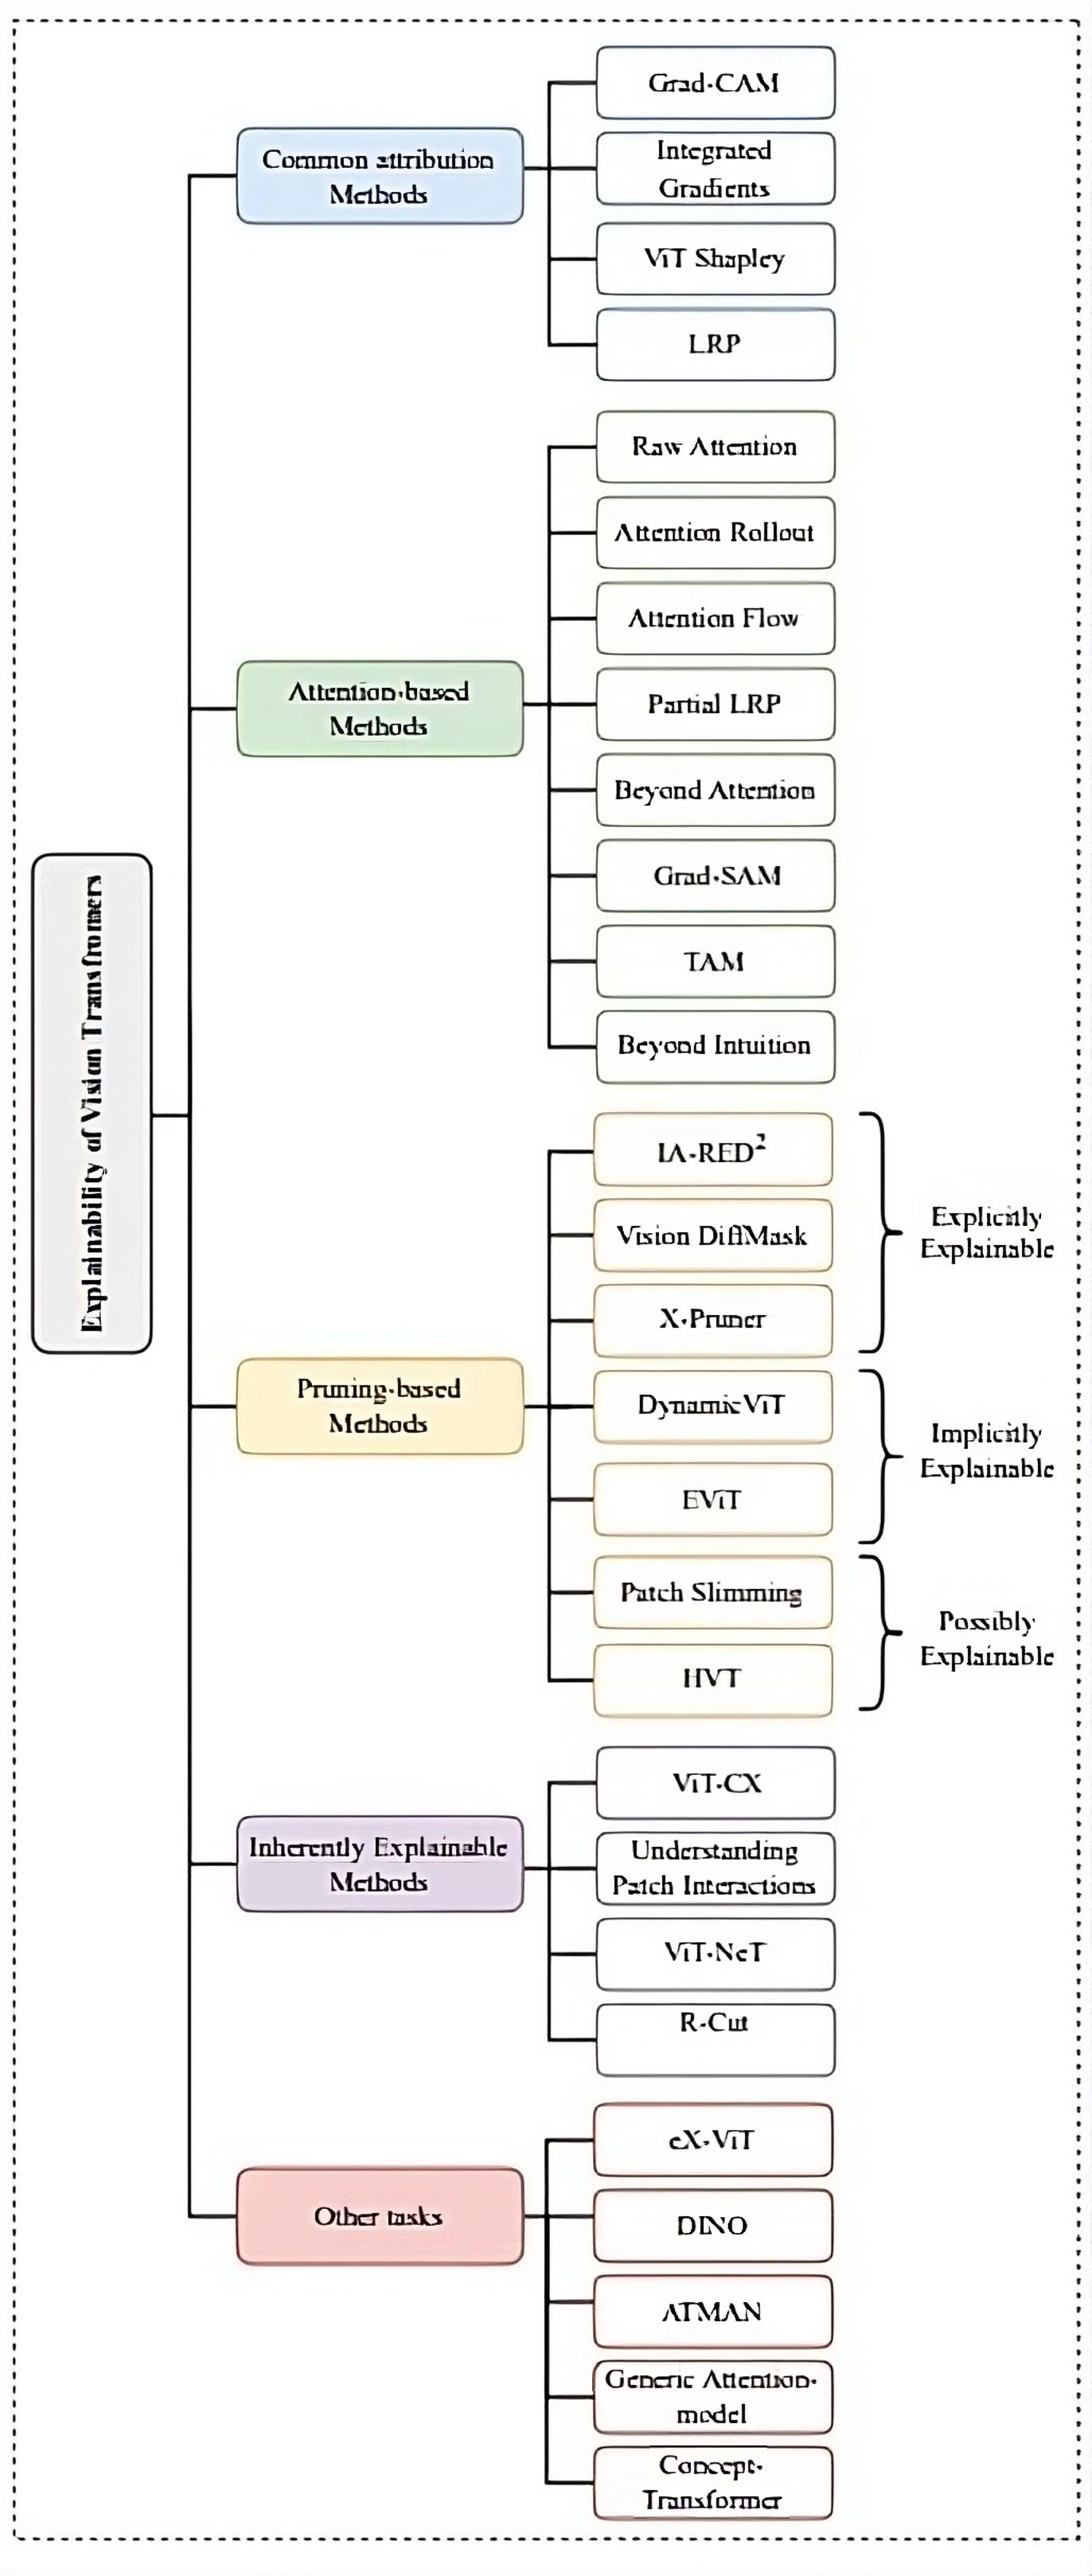
\includegraphics[width=0.6\textwidth]{2/figures/vt2.jpeg}
		\caption{ Taxonomía de los métodos de explicabilidad para
			Transformadores de visión (\cite{tecnica1})}
	\end{center}
\end{figure}

\subsubsection{ Métodos basados en atención}
Los métodos basados en atención aprovechan el mecanismo de atención de los modelos para identificar y priorizar las partes más relevantes de una secuencia de entrada. Muchos enfoques existentes se centran en utilizar los pesos de atención o el conocimiento codificado en ellos para explicar el comportamiento del modelo. En aplicaciones basadas en visión, la visualización de los pesos de atención puede ser útil para identificar patrones de atención, aunque puede volverse menos confiable a medida que la red crece más profunda y más compleja. Para superar estos desafíos, se han introducido dos métodos: "Attention Rollout" y "Attention Flow", que cuantifican el flujo de información y aproximan la atención a los tokens de entrada de manera más holística. Estos métodos tienen sus limitaciones, por lo que se han desarrollado enfoques adicionales, como "GradSAM" y "Transition Attention Maps" (TAM), que aplican funciones como gradientes a los pesos de atención para mejorar la explicación de las predicciones del modelo. Además, el marco "Beyond Intuition" propone una aproximación novedosa para aproximarse a las contribuciones de los tokens, operando en dos etapas: percepción de atención y retroalimentación de razonamiento.

\begin{table}[htbp]
	\centering
	\caption{Methods for Attention-based Class-specific Multi-modality}
	\label{tab:methods}
	\begin{tabular}{llllll}
		\toprule
		Method & Attention & Class-specific & Multi-modality & Backbone & Date \\
		\midrule
		Raw Attention & Yes & No & No & VIT, DEIT & 2017 \\
		Attention Rollout & Yes & No & No & VIT, DEIT & 2020 \\
		Attention Flow & Yes & No & No & VIT, DEIT & 2020 \\
		Partial LRP & Yes & No & No & VIT & 2019 \\
		Grad-SAM & Yes & Yes & No & VIT & 2021 \\
		Beyond Attention & Yes & Yes & Yes & VIT & 2021 \\
		TAM & Yes & Yes & No & VIT, DEIT & 2021 \\
		Beyond Intuition & Yes & Yes & Yes & BERT, VIT, CLIP & 2023 \\
		\bottomrule
	\end{tabular}
\end{table}

\begin{figure}[H]
	\begin{center}
		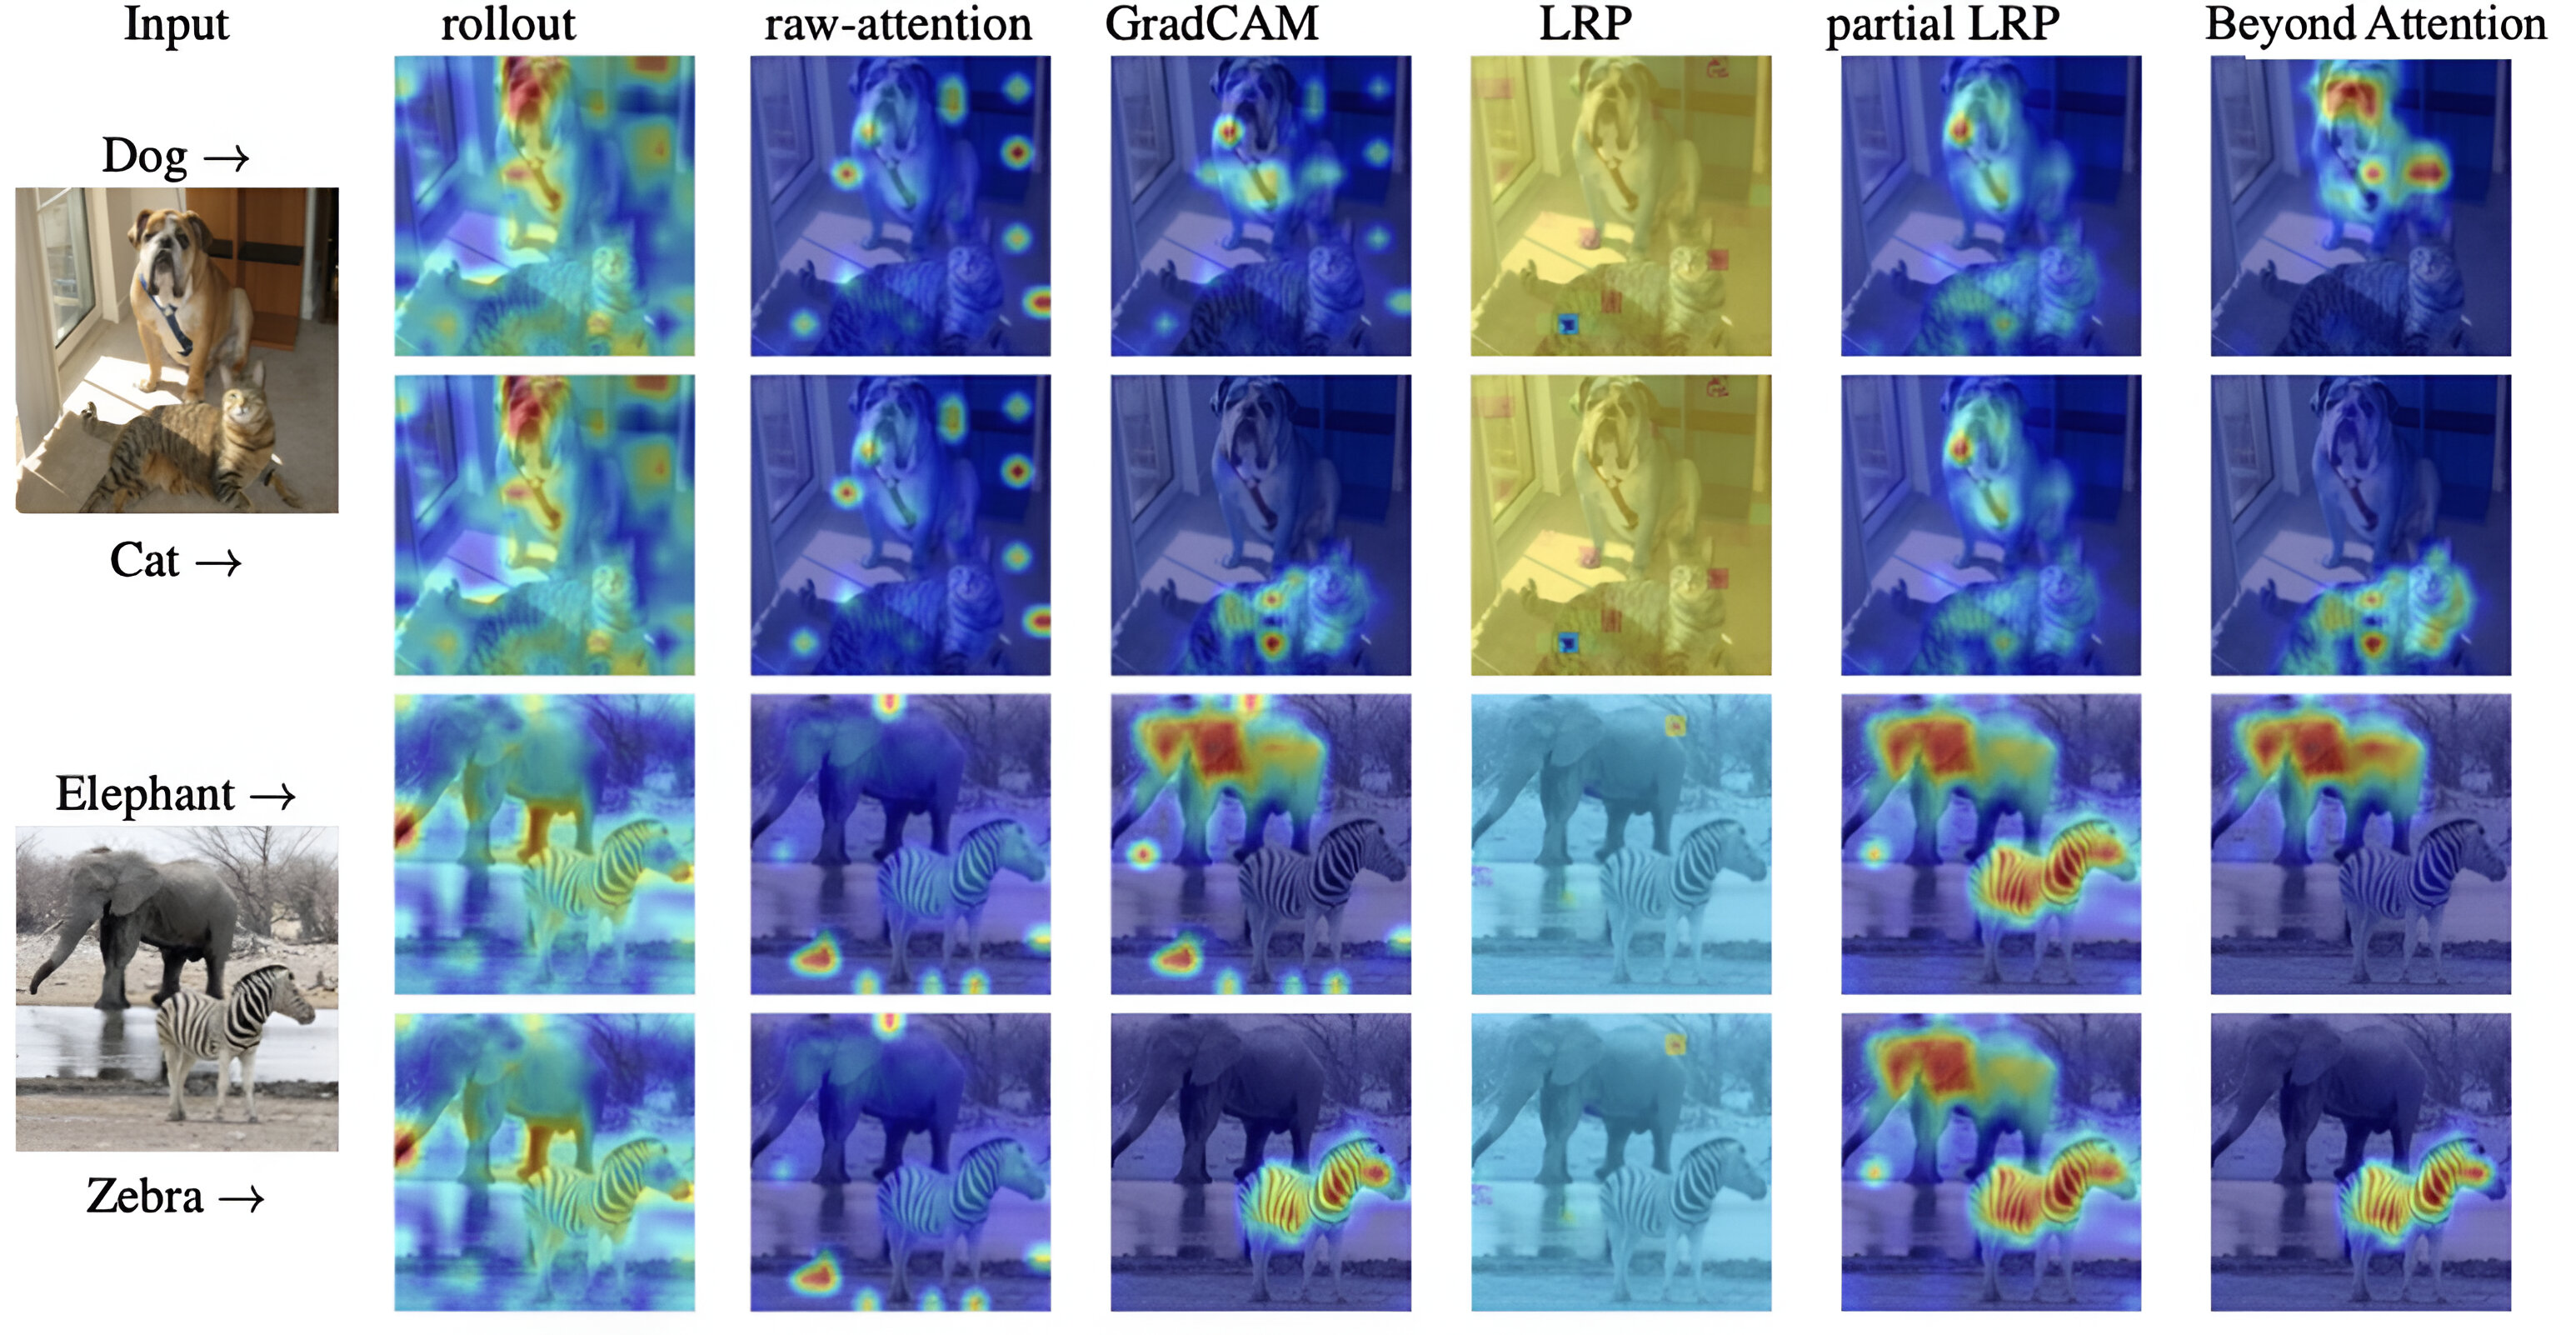
\includegraphics[width=1\textwidth]{2/figures/vt4.jpeg}
		\caption{ Visualizaciones específicas de clase de varios métodos basados en la atención, para cada imagen se pueden ver resultados de dos clases diferentes(\cite{tecnica1})}
	\end{center}
\end{figure}

\subsubsection{ Métodos basados en la poda} 
Los métodos basados en poda son una poderosa herramienta utilizada para optimizar la eficiencia y complejidad de los transformers. Estos métodos intentan eliminar elementos redundantes o poco informativos como tokens, parches, bloques o cabezas de atención de las redes. Algunos de estos métodos están explícitamente desarrollados con fines de explicabilidad, mientras que otros se centran principalmente en mejorar la eficiencia y no tienen como objetivo específico la explicabilidad. Sin embargo, estudios indican que las técnicas del segundo grupo también pueden impactar positivamente la explicabilidad del modelo. Se pueden categorizar los métodos de poda basados en ViT en tres grupos: métodos explícitamente explicables, implícitamente explicables y posiblemente explicables.

Entre los métodos de poda explícitamente explicables, hay varios enfoques notables que buscan proporcionar modelos menos complejos y más interpretables. Por ejemplo, el método IA-RED2 busca encontrar el equilibrio perfecto entre eficiencia e interpretabilidad al eliminar dinámicamente los parches menos informativos, lo que resulta en una velocidad significativamente mayor con una pérdida mínima de precisión. Otro método, X-Pruner, está diseñado específicamente para podar unidades menos significativas, logrando importantes ahorros computacionales sin perder precisión.

Por otro lado, los métodos de poda implícitamente explicables, como el marco DynamicViT, están diseñados principalmente para mejorar la eficiencia de la red, pero también pueden mejorar la explicabilidad al localizar las partes críticas de la imagen que contribuyen más a la clasificación. EViT es otro enfoque innovador que reorganiza los tokens de una imagen basándose en el concepto de atención, manteniendo los tokens más relevantes mientras fusiona los menos atentos en un solo token, lo que reduce los costos computacionales sin comprometer la precisión del modelo. Estos métodos mejoran la interpretabilidad y ofrecen una comprensión más clara de las decisiones del modelo.   

\begin{table}[H]
	\centering
	\caption{ Comparacion de metodos de poda basados en DeiT-S Touvron en 2021 en el conjunto de datos ImageNet}
	\label{tab:pruning_comparison}
	\begin{tabular}{lccc}
		\toprule
		Método de poda & GFLOPs $\downarrow$ (\%) & TOP-1 Exactitud $\downarrow$ (\%) & Rendimiento $\uparrow$ (\%) \\
		\midrule
		IA-RED2        & --                        & 0.7                               & 46                            \\
		DynamicViT     & 37                        & 0.5                               & 54                            \\
		EViT           & 35                        & 0.3                               & 50                            \\
		
		HVT            & 47.8                      & 1.8                               & --                            \\
		\bottomrule
	\end{tabular}
\end{table}


Los métodos posiblemente explicables son enfoques adicionales de poda que, aunque inicialmente no se diseñaron para mejorar la interpretabilidad de ViT, podrían ofrecer un potencial para investigar su impacto en la explicabilidad de los modelos. Por ejemplo, Patch Slimming es un algoritmo novedoso que acelera ViTs al dirigirse a los parches redundantes en las imágenes de entrada, lo que potencialmente destaca características visuales importantes y mejora la interpretabilidad. Otro enfoque, Hierarchical Visual Transformer (HVT), mejora la escalabilidad y el rendimiento de ViTs al reducir gradualmente la longitud de la secuencia a medida que aumenta la profundidad del modelo. Aunque estos métodos se han evaluado principalmente en términos de eficiencia, existe una brecha significativa en la literatura en cuanto a la evaluación de su explicabilidad. En contraste, los métodos inherentemente explicables, como ViT-CX, se centran en desarrollar modelos que puedan explicarse a sí mismos, utilizando herramientas interpretables como mapas de saliencia para proporcionar explicaciones más significativas.

\begin{figure}[H]
	\begin{center}
		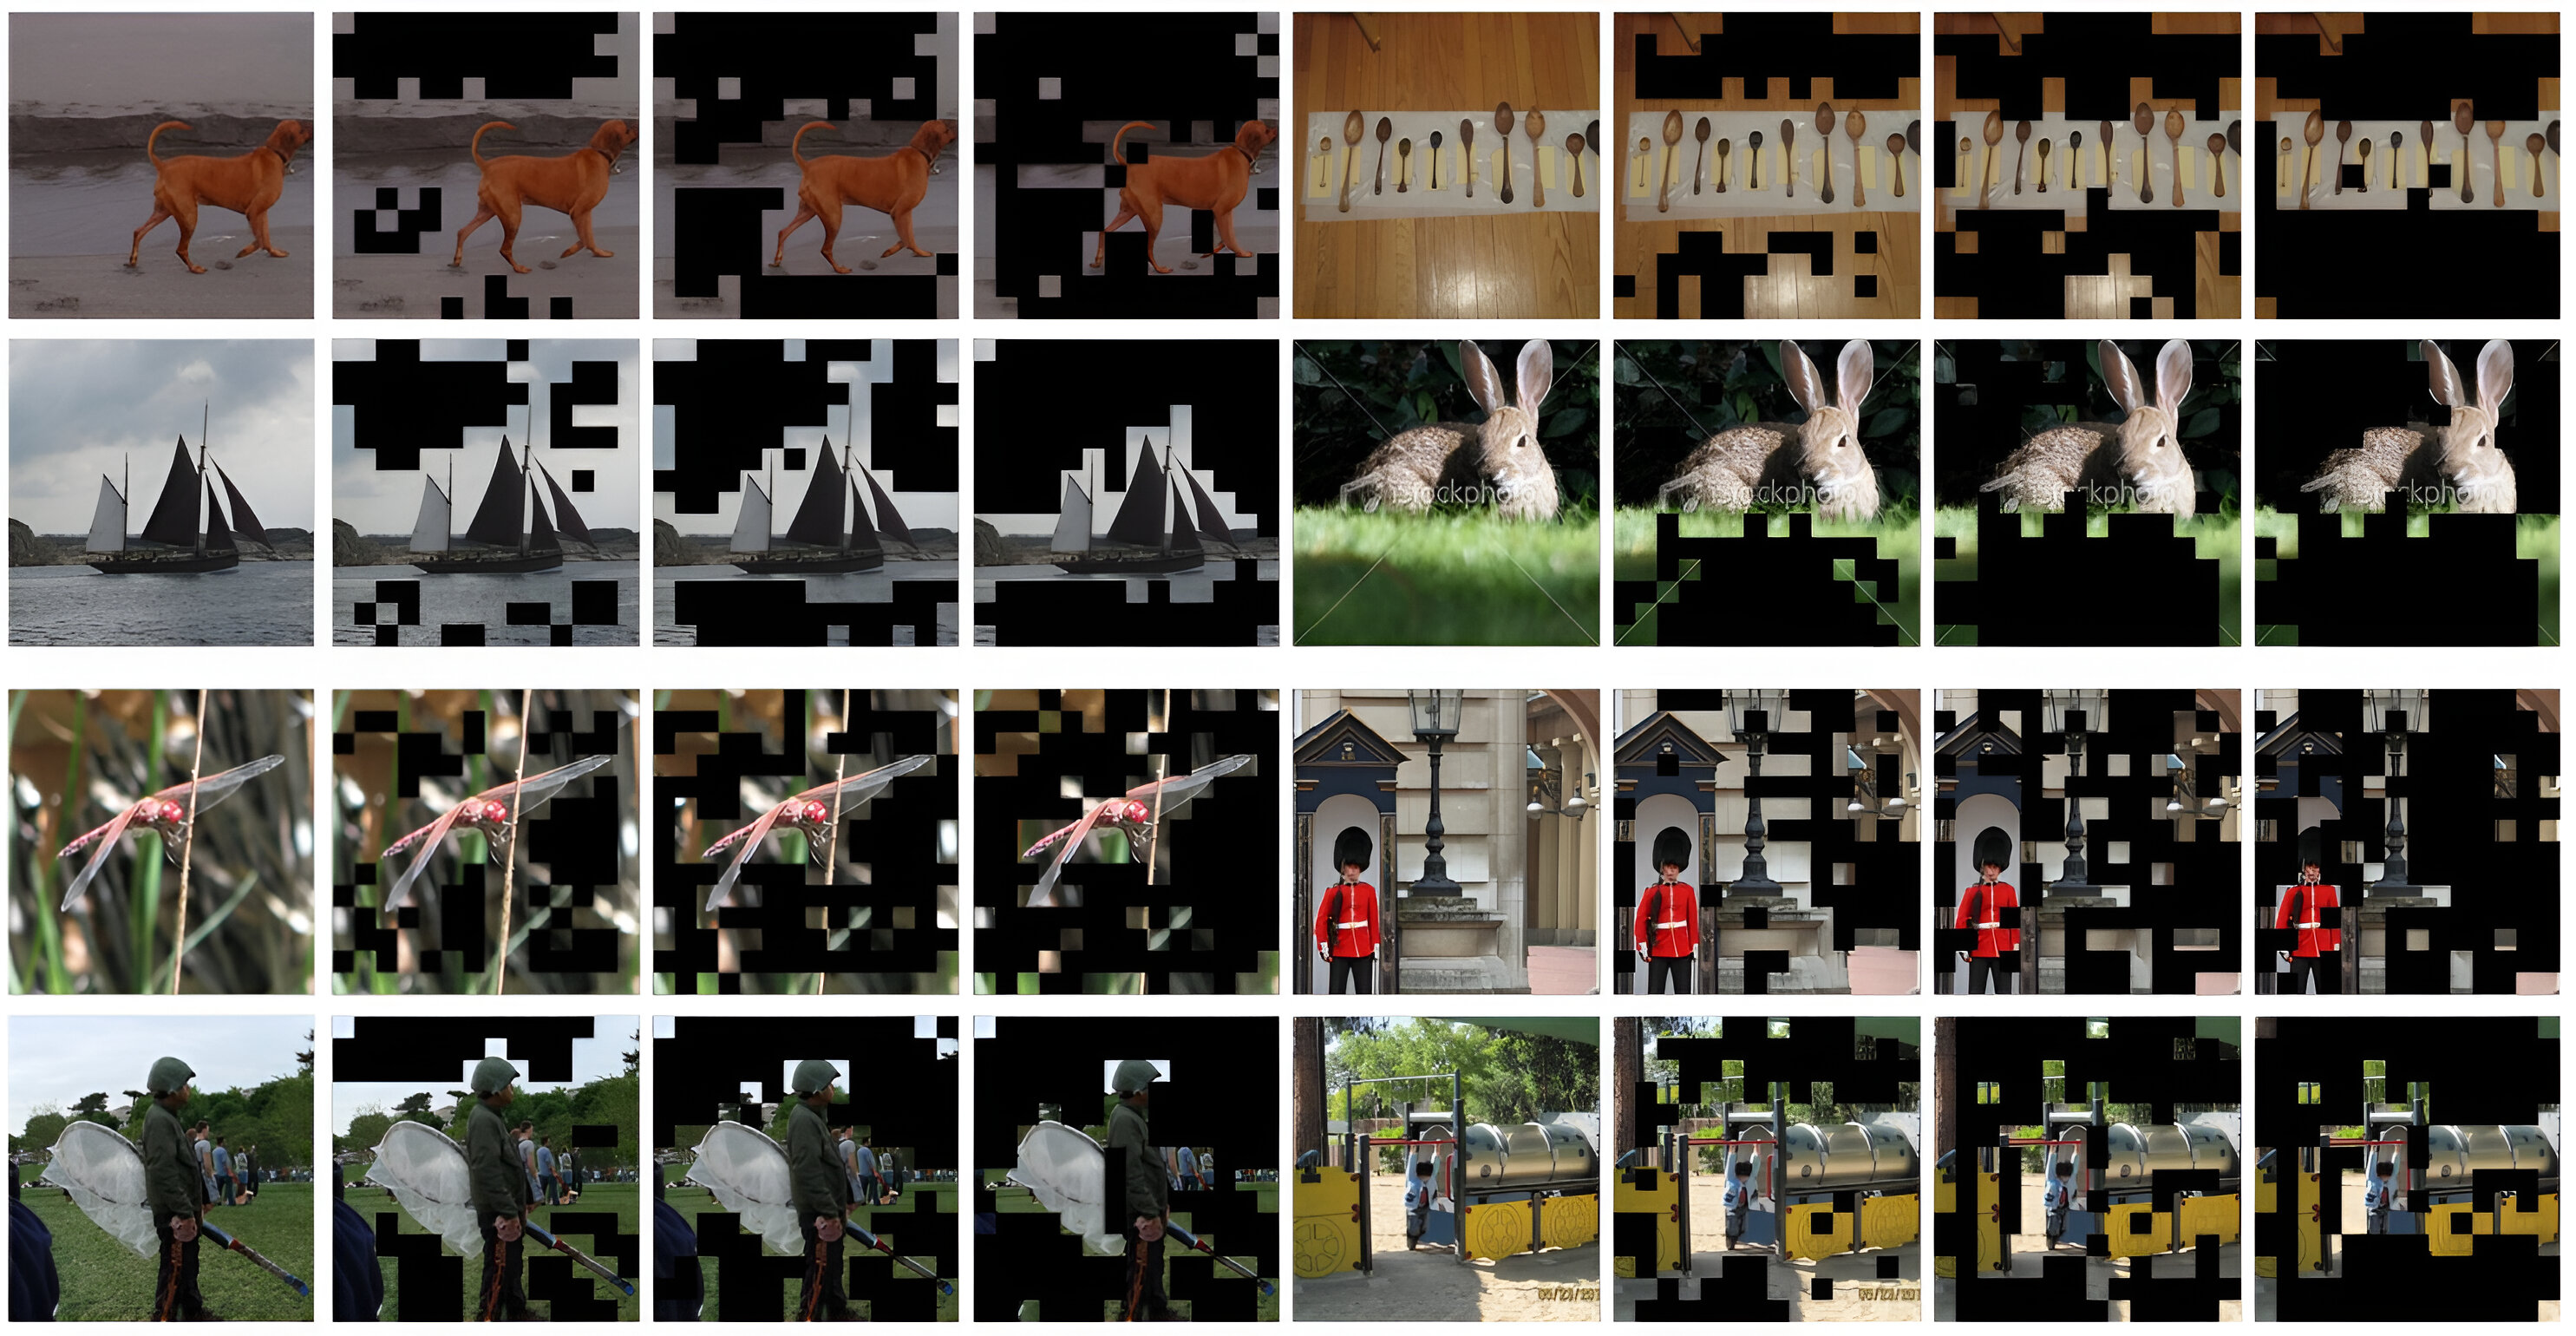
\includegraphics[width=1\textwidth]{2/figures/vt6.jpeg}
		\caption{Visualización de tokens desatentos en EViT-DeiT-S con 12 capas; Se puede ver que las fichas de falta de atención se fusionan gradualmente (como se representa mediante áreas enmascaradas) o se eliminan, mientras que las fichas más informativas se conservan. Esto permite a los ViT centrarse en tokens específicos de clase en imágenes, lo que conduce a una mejor interpretabilidad(\cite{tecnica1})}
	\end{center}
\end{figure}


\subsubsection{Evaluación de explicación}
En secciones anteriores, presentamos varias técnicas de explicación desarrolladas específicamente para aplicaciones basadas en ViT. Sin embargo, evaluar qué tan bien estas técnicas representan el proceso de razonamiento de un modelo presenta diferentes desafíos. Para abordar esta preocupación, la literatura sugiere una serie de criterios evaluativos, que ayudan a seleccionar y diseñar la técnica de explicabilidad más apropiada. A continuación, se resumen estos criterios:
\begin{itemize}
	\item \textbf{Deletion and Insertion:} Se utilizan para evaluar la fidelidad de un mapa de saliencia al modelo objetivo. Calculan cómo el mapa de saliencia identifica los píxeles más influyentes para la predicción del modelo.
	\item \textbf{Effective Complexity:} Evalúa el número de atribuciones que superan un umbral, indicando la importancia o insignificancia de las características correspondientes.
	
	\item \textbf{Faithfulness:} Método para evaluar la calidad de las atribuciones de características sin intervención humana, midiendo cuán precisamente las atribuciones de características se alinean o correlacionan con las predicciones del modelo.
	
	\item \textbf{(In)fidelity:} Se utiliza para evaluar qué tan bien una explicación captura los cambios en las predicciones de un modelo cuando la entrada sufre perturbaciones significativas.
	
	\item \textbf{Intersection over Union (IoU) test:} Métrica estándar para evaluar el rendimiento de los detectores y seguidores de objetos, que también se ha utilizado para evaluar métodos de explicabilidad midiendo la superposición entre los mapas de explicabilidad predichos y las cajas delimitadoras de la verdad terrenal de los objetos de interés.
	
	\item \textbf{Perturbation Tests:} Funcionan al enmascarar gradualmente tokens de entrada basándose en las explicaciones proporcionadas por el método de explicabilidad dado.
	
	\item \textbf{Pointing Game:} Método para evaluar los mapas de saliencia de la explicación en comparación con las cajas delimitadoras anotadas por humanos.
	
	\item \textbf{Segmentation Tests:} Consideran cada visualización como una segmentación suave de la imagen y las comparan con la verdad terrenal proporcionada en el conjunto de datos.
	
	\item \textbf{Sensitivity:} Evalúa cómo varían las explicaciones con pequeñas perturbaciones en la entrada.
	
	\item \textbf{Sensitivity-n:} Propuesto para probar valores de atribución específicos en lugar de considerar solo las clasificaciones de importancia.
\end{itemize}

\begin{figure}[H]
	\begin{center}
		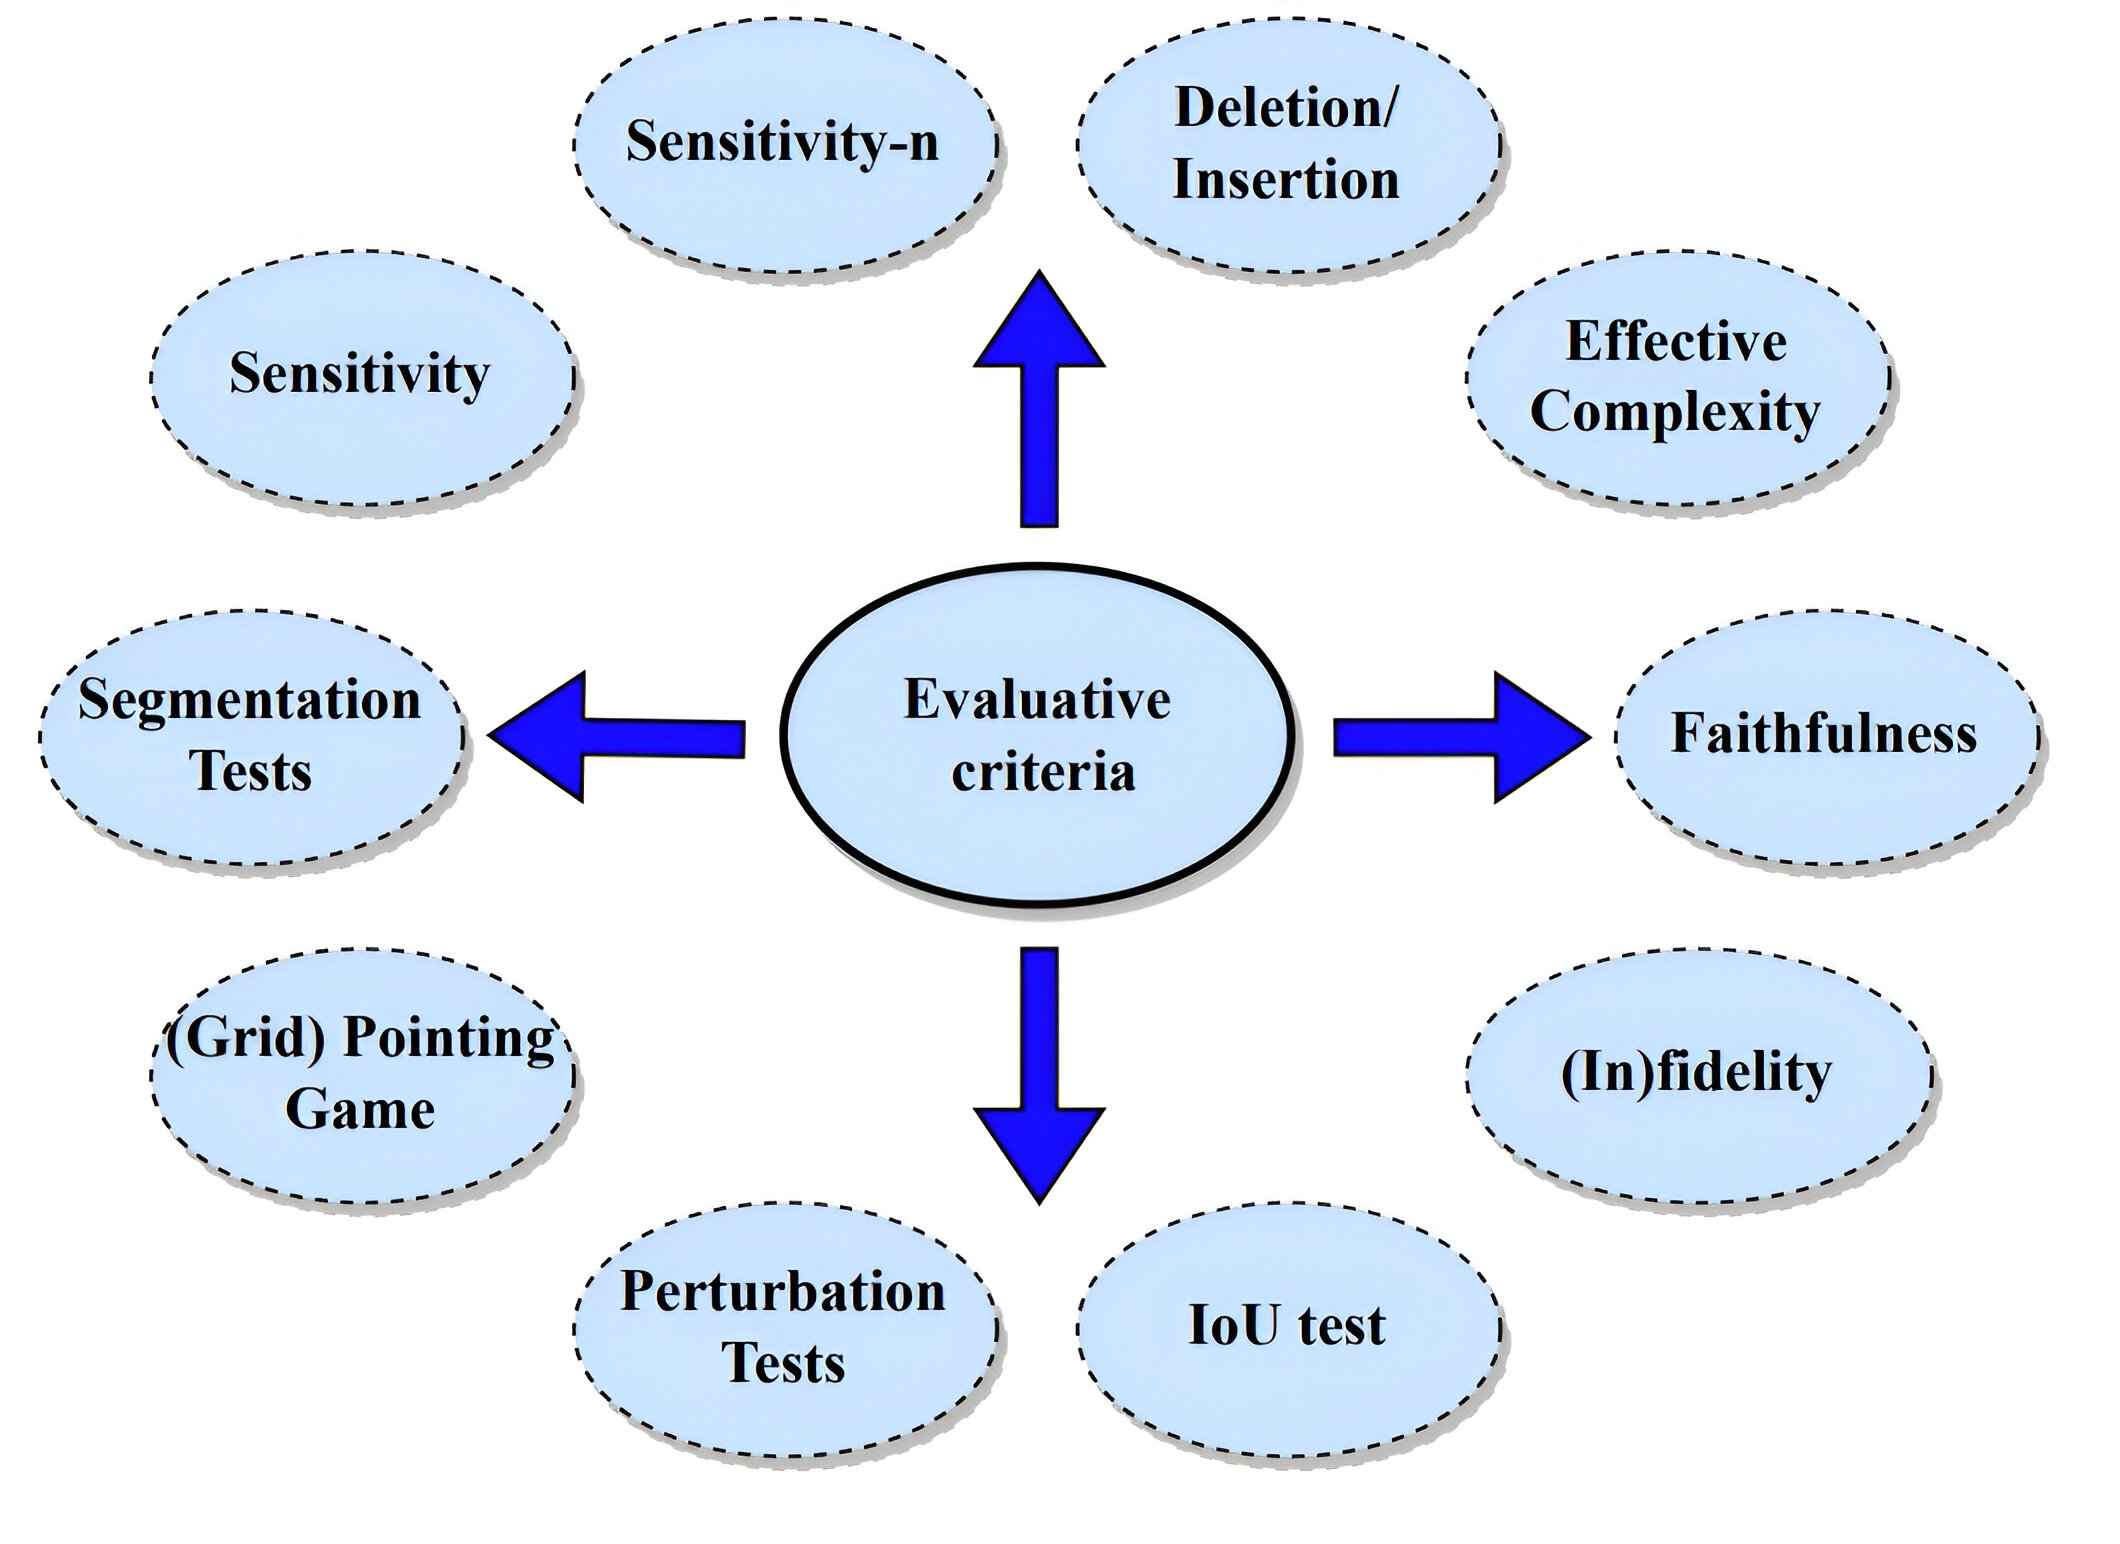
\includegraphics[width=1\textwidth]{2/figures/vt8.jpeg}
		\caption{Diferentes criterios para evaluar los métodos de explicabilidad en aplicaciones basadas en la visiónt(\cite{tecnica1})}
	\end{center}
\end{figure}

\subsubsection{Conclusión}

En resumen, este trabajo ofrece una visión completa de las técnicas de explicabilidad propuestas para los transformers visuales. Hemos proporcionado una taxonomía de los métodos basada en sus motivaciones, estructuras y escenarios de aplicación, categorizándolos en cinco grupos. Además, detallamos los criterios de evaluación de la explicabilidad, así como las herramientas y marcos de trabajo utilizados. Por último, discutimos varios problemas esenciales pero poco explorados para mejorar la explicabilidad de los transformers visuales y sugerimos direcciones de investigación potenciales para futuras inversiones. Esperamos que este artículo de revisión ayude a los lectores a comprender mejor los mecanismos internos de los transformers visuales, así como a resaltar problemas abiertos para trabajos futuros.

\subsection{You Only Look One (YOLO): You Only Look Once: Unified, Real-Time Object Detection \citep*{tecnica4}}
YOLO trata la detección de objetos como un problema de regresión, prediciendo cuadros delimitadores y probabilidades de clase directamente de imágenes completas en una sola evaluación. Esto permite una arquitectura muy rápida, procesando imágenes en tiempo real a 45 cuadros por segundo, con Fast YOLO alcanzando 155 cuadros por segundo. Aunque YOLO puede cometer más errores de localización, es menos propenso a falsos positivos de fondo y generaliza mejor a diferentes dominios como el arte.
\subsubsection{Introducción}
En la detección de objetos, los sistemas actuales utilizan enfoques complejos que reutilizan clasificadores para detectar objetos, lo que los hace lentos y difíciles de optimizar. En contraste, el enfoque de YOLO reframes la detección como un problema de regresión única, lo que permite predecir objetos y sus ubicaciones directamente desde los píxeles de la imagen en una sola evaluación. Esto ofrece varias ventajas: en primer lugar, YOLO es extremadamente rápido, con una tasa de ejecución de hasta 150 cuadros por segundo, lo que permite el procesamiento de video en tiempo real con una latencia mínima. Además, YOLO considera globalmente la imagen al realizar predicciones, lo que le permite codificar implícitamente información contextual sobre las clases y su apariencia. Por último, YOLO aprende representaciones generalizables de objetos, lo que lo hace menos propenso a descomponerse al aplicarse en nuevos dominios o entradas inesperadas. Sin embargo, YOLO aún se queda atrás en precisión en comparación con otros sistemas de detección de vanguardia, especialmente en la localización precisa de objetos pequeños.

\begin{figure}[H]
	\begin{center}
		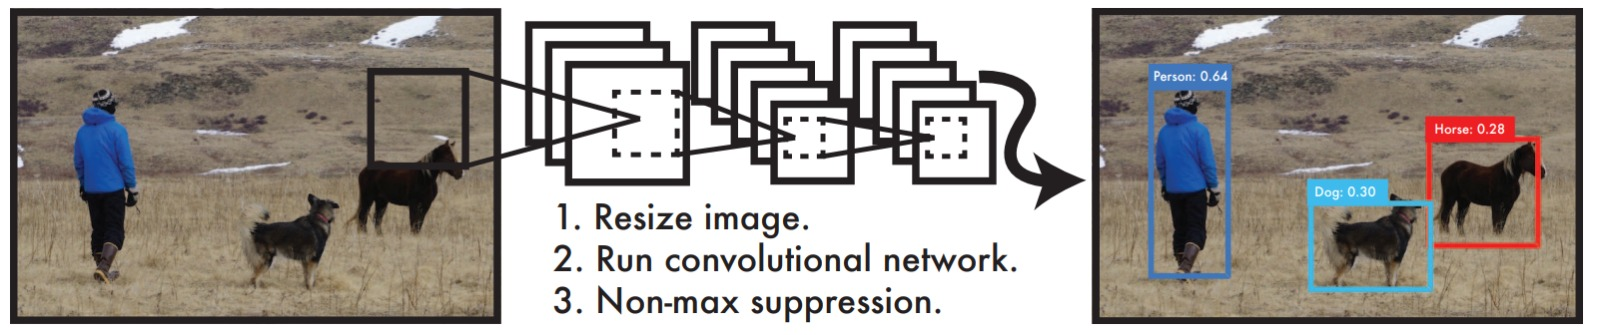
\includegraphics[width=1\textwidth]{2/figures/yolo1.jpeg}
		\caption{El sistema de detección YOLO. Procesamiento de imágenes
			con YOLO es simple y directo. Nuestro sistema (1) cambia de tamaño
			la imagen de entrada a 448 × 448, (2) ejecuta una única red convolucional en la imagen y (3) establece umbrales para las detecciones resultantes mediante
			La confianza del modelo.(\cite{tecnica4})}
	\end{center}
\end{figure}
\subsubsection{Detección unificada}
El método fusiona todos los elementos de detección de objetos en una única red neuronal. Esta red utiliza características de toda la imagen para predecir simultáneamente las cajas delimitadoras y las clases de objetos, permitiendo un entrenamiento de extremo a extremo y velocidades en tiempo real sin perder precisión. La imagen se divide en una cuadrícula $S \times S$, donde cada celda detecta un objeto si su centro cae en ella. Cada celda predice $B$ cajas delimitadoras y sus puntuaciones de confianza, indicando la certeza del modelo sobre la presencia y precisión del objeto, además de $C$ probabilidades de clase condicionales. Durante la prueba, se combinan estas probabilidades y las predicciones de confianza para obtener puntuaciones específicas de clase para cada caja.

\begin{figure}[H]
	\begin{center}
		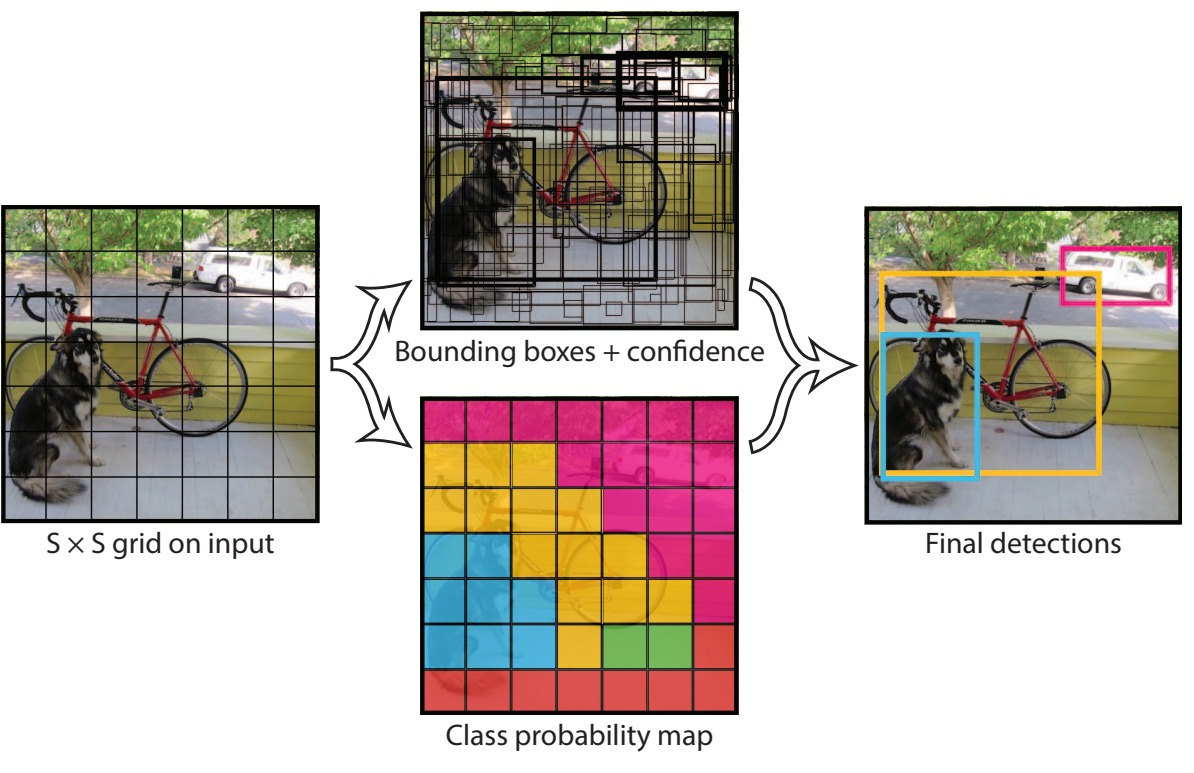
\includegraphics[width=1\textwidth]{2/figures/yolo2.jpeg}
		\caption{El sistema aborda la detección como un problema de regresión, donde la imagen se divide en una cuadrícula S × S. Para cada celda de esta cuadrícula, se predicen cuadros delimitadores, confianza asociada con esos cuadros y probabilidades de clase. Estas predicciones se codifican en un tensor con dimensiones S × S × (B x 5 + C). (\cite{tecnica4})}
	\end{center}
\end{figure}

Este modelo, una red neuronal convolucional, se evalúa en el conjunto de datos de detección PASCAL VOC. Utiliza capas convolucionales para extraer características de la imagen y capas completamente conectadas para predecir las salidas. Basado en GoogLeNet, consta de 24 capas convolucionales y 2 capas completamente conectadas. En lugar de módulos de inception, emplea capas de reducción de 1 × 1 seguidas de convoluciones de 3 × 3. Además, desarrolla una versión rápida de YOLO con menos capas convolucionales y filtros para mejorar la detección rápida de objetos.

\begin{figure}[H]
	\begin{center}
		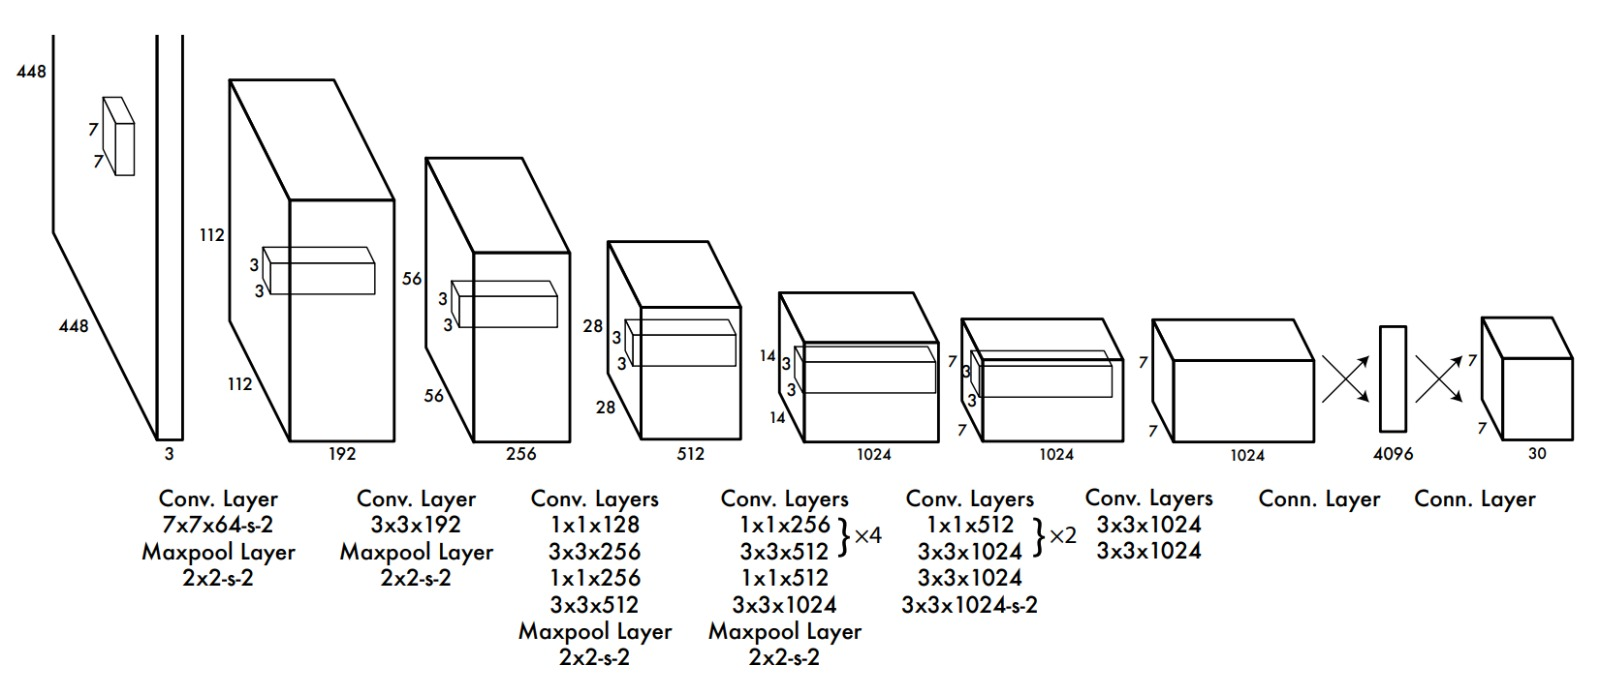
\includegraphics[width=1\textwidth]{2/figures/yolo3.jpeg}
		\caption{La red de detección consta de 24 capas convolucionales y 2 capas completamente conectadas. Se utilizan capas convolucionales de 1 × 1 para reducir el espacio de características de las capas anteriores y se preentrenan en la tarea de clasificación de ImageNet a la mitad de la resolución (224 × 224), incrementando la resolución para la detección. (\cite{tecnica4})}
	\end{center}
\end{figure}

\paragraph{Training} 
Las capas convolucionales se preentrenan en el conjunto de datos ImageNet de 1000 clases, logrando una precisión top-5 del 88\%. La red se convierte para la detección, aumentando la resolución de entrada de 224 × 224 a 448 × 448 para capturar detalles. La capa final predice las probabilidades de clase y las coordenadas de las cajas delimitadoras, optimizando para el error cuadrático medio. Se entrena durante aproximadamente 135 épocas en los conjuntos de datos de PASCAL VOC 2007 y 2012, utilizando un tamaño de lote de 64 y una tasa de aprendizaje variable. Durante la inferencia, predice detecciones con una sola evaluación de red, empleando supresión no máxima para corregir múltiples detecciones..

\paragraph{Limitaciones de YOLO}
YOLO impone restricciones espaciales significativas en las predicciones de las cajas delimitadoras. Cada celda de la cuadrícula solo puede predecir dos cajas y asignar una única clase, lo que limita la capacidad del modelo para detectar objetos cercanos, especialmente objetos pequeños que aparecen en grupos, como bandadas de pájaros.

Dado que el modelo aprende de los datos, enfrenta dificultades para generalizar a objetos con relaciones de aspecto nuevas o inusuales. Además, utiliza características relativamente gruesas para predecir las cajas delimitadoras debido a múltiples capas de muestreo descendente desde la imagen de entrada.

La función de pérdida utilizada durante el entrenamiento no distingue entre errores en cajas delimitadoras pequeñas y grandes, lo que puede llevar a una penalización desproporcionada por errores en cajas pequeñas, que tienen un impacto significativo en la evaluación de la superposición de IOU. En consecuencia, las localizaciones incorrectas son la principal fuente de error en nuestro modelo.

\subsubsection{Experimentos}
Se contrastó YOLO con otros sistemas de detección en tiempo real en PASCAL VOC 2007, revelando que YOLO y Fast R-CNN muestran distintos perfiles de errores. Asimismo, se evidenció la capacidad de YOLO para generalizar mejor en nuevos dominios, como conjuntos de datos de obras de arte, en comparación con otros métodos actuales en VOC 2012.

Dentro del ámbito de la detección de objetos en tiempo real, la mayoría de los esfuerzos de investigación se enfocan en mejorar la velocidad de los procesos estándar de detección. YOLO fue evaluado frente a otros métodos, resaltando su rapidez y precisión. Se introdujo una versión más ágil, Fast YOLO, que sobrepasa considerablemente a los enfoques previos en cuanto a precisión y velocidad.

Además, se examinaron otros métodos como Fastest DPM, R-CNN menos R, Fast R-CNN y Faster R-CNN, destacando sus velocidades y precisión en comparación con YOLO. Sin embargo, ninguno de ellos logra igualar el desempeño en tiempo real de YOLO.

\begin{table}[H]
	\centering
	\caption{Comparación de Detectores en Tiempo Real y Menos que en Tiempo Real}
	\label{tab:real-time-detectors}
	\begin{tabular}{|l|l|l|l|}
		\hline
		\textbf{Detector} & \textbf{Entrenamiento} & \textbf{mAP} & \textbf{FPS} \\ \hline
		100Hz DPM  & 2007 & 16.0 & 100 \\ \hline
		30Hz DPM  & 2007 & 26.1 & 30 \\ \hline
		Fast YOLO & 2007+2012 & 52.7 & 155 \\ \hline
		YOLO & 2007+2012 & 63.4 & 45 \\ \hline
		\multicolumn{4}{|c|}{\textbf{Menos que en Tiempo Real}} \\ \hline
		Fastest DPM  & 2007 & 30.4 & 15 \\ \hline
		R-CNN Minus R  & 2007 & 53.5 & 6 \\ \hline
		Fast R-CNN  & 2007+2012 & 70.0 & 0.5 \\ \hline
		Faster R-CNN VGG-16  & 2007+2012 & 73.2 & 7 \\ \hline
		YOLO VGG-16 & 2007+2012 & 66.4 & 21 \\ \hline
	\end{tabular}
\end{table}


Para examinar las diferencias entre YOLO y detectores de última generación, se realizó un análisis detallado de los resultados en VOC 2007, comparando YOLO con Fast R-CNN. Usando la metodología de Hoiem, se clasificaron las predicciones en categorías basadas en el tipo de error:

\begin{itemize}
	\item \textbf{Correcto}: clase correcta e IOU > 0.5
	\item \textbf{Localización}: clase correcta, 0.1 < IOU < 0.5
	\item \textbf{Similar}: clase similar, IOU > 0.1
	\item \textbf{Otro}: clase incorrecta, IOU > 0.1
	\item \textbf{Fondo}: IOU < 0.1 para cualquier objeto
\end{itemize}

La Figura \ref{fig:error_analysis} muestra el desglose promedio de cada tipo de error en las 20 clases. YOLO tiene más errores de localización que cualquier otra fuente combinada, mientras que Fast R-CNN comete menos errores de localización pero muchos más errores de fondo. El 13.6\% de las detecciones de Fast R-CNN son falsos positivos sin objetos, siendo casi 3 veces más propenso a predecir detecciones de fondo en comparación con YOLO.

\begin{figure}[h]
	\centering
	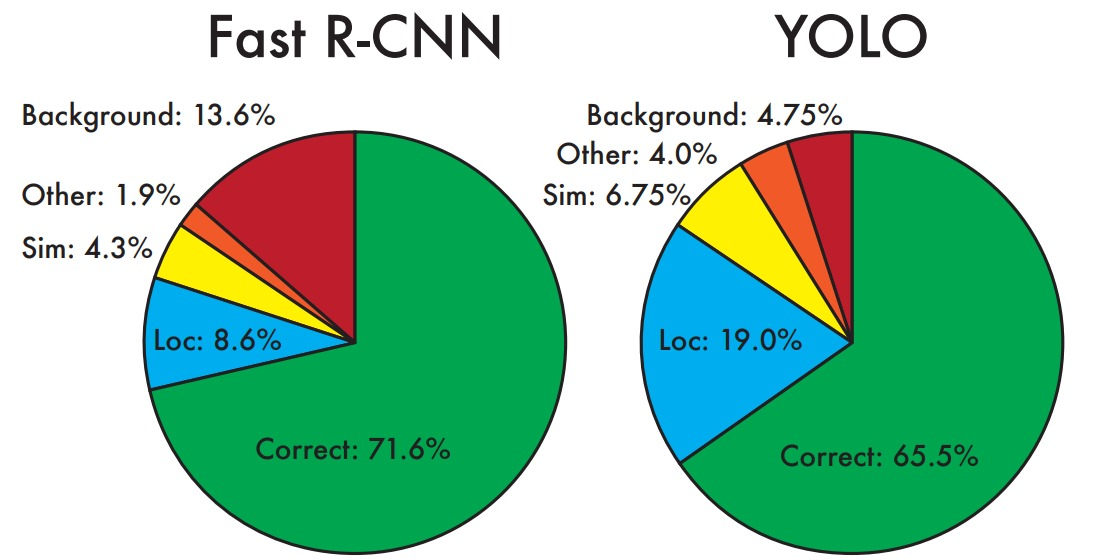
\includegraphics[width=0.8\textwidth]{2/figures/yolo4.jpeg}
	\caption{Análisis de Errores: Fast R-CNN vs. YOLO. Estos gráficos muestran el porcentaje de errores de localización y de fondo en las principales detecciones de varias categorías.}
	\label{fig:error_analysis} 
\end{figure}

YOLO comete muchos menos errores de fondo que Fast R-CNN. Al usar YOLO para eliminar las detecciones de fondo de Fast R-CNN, se obtiene una mejora significativa en el rendimiento. Por cada cuadro delimitador que predice R-CNN, se verifica si YOLO predice un cuadro similar. Si es así, se le da un impulso a esa predicción basado en la probabilidad predicha por YOLO y la superposición entre los dos cuadros.

El mejor modelo de Fast R-CNN alcanza un mAP de 71.8\% en el conjunto de prueba de VOC 2007. Cuando se combina con YOLO, su mAP aumenta a 75.0\%, con una ganancia de 3.2\%, como se muestra en la Tabla \ref{table:combination}.

\begin{table}[h]
	\centering
	\begin{tabular}{|l|c|c|c|}
		\hline
		\textbf{Modelo} & \textbf{mAP} & \textbf{Combinado} & \textbf{Ganancia} \\
		\hline
		Fast R-CNN & 71.8 & - & - \\
		Fast R-CNN (2007 data) & 66.9 & 72.4 & 0.6 \\
		Fast R-CNN (VGG-M) & 59.2 & 72.4 & 0.6 \\
		Fast R-CNN (CaffeNet) & 57.1 & 72.1 & 0.3 \\
		YOLO & 63.4 & 75.0 & 3.2 \\
		\hline
	\end{tabular}
	\caption{Experimentos de combinación de modelos en VOC 2007. Se examina el efecto de combinar varios modelos con la mejor versión de Fast R-CNN.}
	\label{table:combination}
\end{table}

El aumento de rendimiento no es simplemente un subproducto de la combinación de modelos, ya que la combinación de diferentes versiones de Fast R-CNN produce beneficios pequeños (entre 0.3 y 0.6\%). En cambio, la eficacia de YOLO se debe a que comete diferentes tipos de errores en las pruebas, lo que mejora significativamente el rendimiento de Fast R-CNN.


\subsubsection{Detección en Tiempo Real en el Mundo Real}

YOLO es un detector de objetos rápido y preciso, lo que lo hace ideal para aplicaciones de visión por computadora. Se conectó YOLO a una cámara web y se verificó que mantiene el rendimiento en tiempo real, incluyendo el tiempo para capturar imágenes desde la cámara y mostrar las detecciones.

\begin{figure}[h]
	\centering
	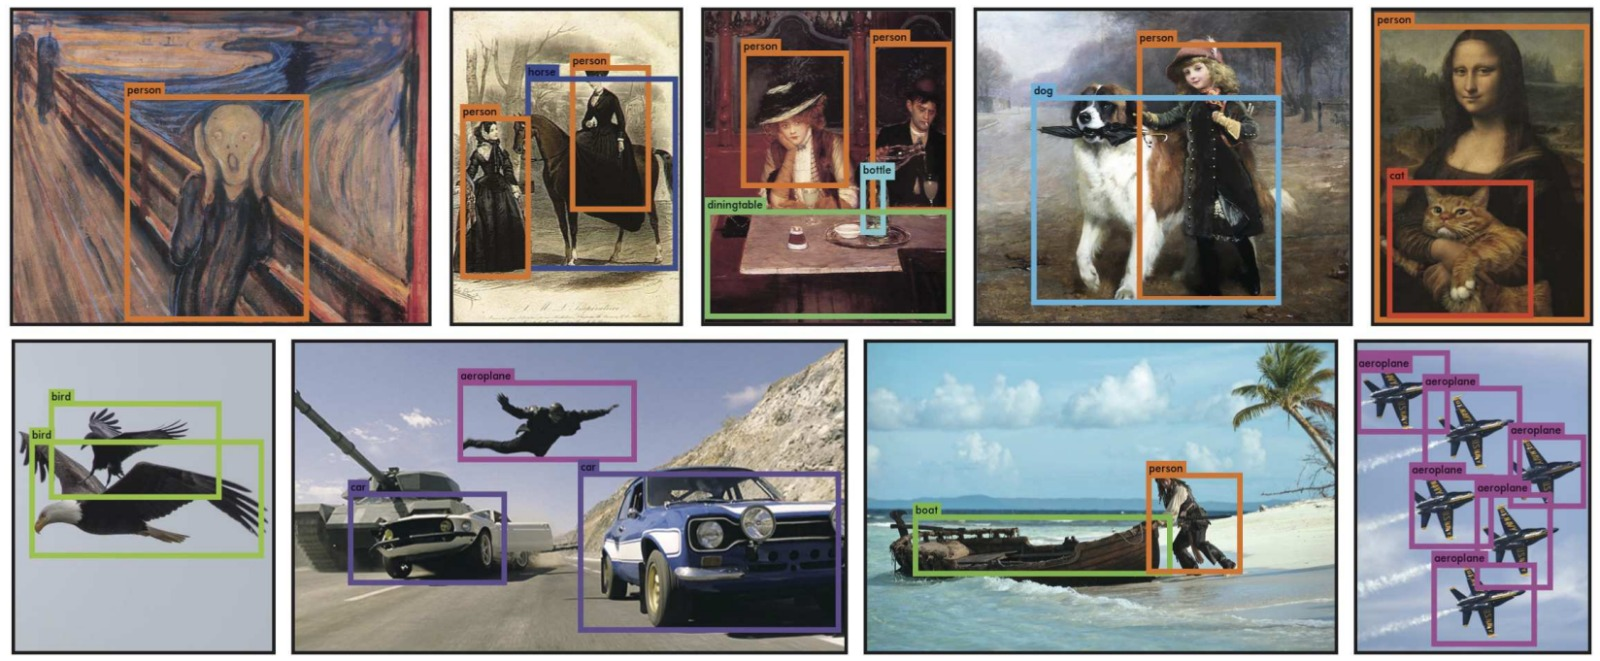
\includegraphics[width=0.8\textwidth]{2/figures/yolo5.jpeg}
	\caption{Resultados cualitativos. YOLO se ejecuta con obras de arte de muestra e imágenes naturales de Internet. Es mayoritariamente exacto, aunque cree que una persona es un avión.(\cite{tecnica4})}
	
\end{figure}

El sistema resultante es interactivo y atractivo. Aunque YOLO procesa imágenes individualmente, cuando se conecta a una cámara web funciona como un sistema de seguimiento, detectando objetos a medida que se mueven y cambian de apariencia.

\subsubsection{Conclusion}
YOLO es un detector de objetos rápido y preciso, ideal para aplicaciones de visión por computadora. Al conectarse a una cámara web, mantiene el rendimiento en tiempo real, incluyendo la captura y visualización de imágenes. El sistema es interactivo y funciona como un sistema de seguimiento, detectando objetos en movimiento

\section{Marco Conceptual}
Para de


%%\chapter{Metodología de la Investigación}
\section{Diseño de la investigación}
En esta sección del documento se explica cuál fue el diseño, el tipo y el enfoque del trabajo de investigación, así como también la población y la muestra. 

\subsection{Tipo de la investigación}
Para determinar el tipo de la investigación, primero fue necesario definir el actual trabajo como Diseño Experimental ya que, según \cite{bk_hernandez2014metodologia} en su libro \citetitle{bk_hernandez2014metodologia}, se pretende establecer el posible efecto de una causa que se manipula. Dentro de esta categoría se clasifica como Diseño Experimental Puro, ya que se manipuló intencionalmente más de una variable independiente (fueron agregadas y/o removidas) con la finalidad de medir el efecto que estas generan en la variable dependiente, el estado final de financiamiento de un proyecto de tecnología en Kickstarter.

\subsection{Enfoque de la investigación}
El presente trabajo tuvo un enfoque cuantitativo ya que, según \cite{bk_hernandez2014metodologia} en su libro \citetitle{bk_hernandez2014metodologia}, este enfoque utiliza la recolección de datos para probar hipótesis con base en la medición numérica y el análisis estadístico, con el fin de establecer pautas de comportamiento y probar teorías. Esto se refleja en los 10 pasos del proceso cuantitativo descritos por el anterior autor y que fueron aplicados en la investigación, desde la concepción de la idea hasta la elaboración del reporte de resultados.

\subsection{Población}
La población fueron todos los proyectos de la web de crowdfunding Kickstarter.

\subsection{Muestra}
La muestra fueron 27,251 proyectos, incluyendo exitosos y fracasados, de la categoría Tecnología, de la web de crowdfunding Kickstarter, entre los periodos 2009 y 2019. Como se mencionó en el Capítulo I, el criterio de la elección de esta categoría se debe a su bajo ratio de éxito de financiamiento en promedio durante los periodos mencionados, los cuales se consideraron hasta el 2019 dado que tomar el año 2020 incurriría en la distorsión del ratio por la coyuntura de la pandemia del Covid-19.

\subsection{Operacionalización de Variables}
En la Tabla \ref{3:table1} se presenta la operacionalización de variables para la investigación.

%\begin{table}[h!]

\begin{longtable}{M{3cm}M{4.2cm}M{3.6cm}M{4.8cm}}
	\caption[Matriz de operacionalización de variables]{Matriz de operacionalización de variables.}
	\label{3:table1}
	\newcommand{\multirot}[1]{\multirow{2}{*}[-8ex]{\rotcell{\rlap{#1}}}}
	\centering
	\small
	\tabularnewline \specialrule{.1em}{.05em}{.05em}
	VARIABLE & DIMENSIÓN & INDICADOR & CÁLCULO
	\\%%[5pt]
	\specialrule{.1em}{.05em}{.05em}
	\multirow{7}{3cm}[-4ex]{\centering Independiente: Aprendizaje Profundo Multimodal} & \multirow{6}{4.2cm}[-1ex]{
	\centering Modelo de Aprendizaje Profundo
	} & \multicolumn{2}{c}{\centering Cantidad de modelos de Aprendizaje Profundo}
   	\\
	\cline{3-4}
	 &  & \multirow{5}{3.6cm}[0ex]{\centering Efectividad de modelos de Aprendizaje Profundo} & Exactitud
	\\
	\cline{4-4}
	 &  &  & Precisión
	\\
	\cline{4-4}
	 &  &  & Área bajo la curva ROC
	\\
	\cline{4-4}
	 &  &  & Sensibilidad
	\\
	\cline{4-4}
	 &  &  & Puntaje F1
	\\%%[10pt]
	\cline{2-4}
	 & Estructura del modelo de Aprendizaje Profundo
	 & \multicolumn{2}{c}{\thead{Complejidad de la estructura de\\ modelos de Aprendizaje Profundo}}
	\\
	\hline
	\multirow{7}{3cm}[-4ex]{\centering Dependiente: Financiamiento de un proyecto} & \multirow{2}{4.2cm}[-2ex]{\centering Crowdfunding} & \multirow{2}{3.6cm}[0ex]{\centering Estado de financiamiento de un proyecto} & $Exitoso = Meta \leq Contribuci\acute{o}n$ \\
	\cline{4-4}
	 &  &  &
	 $Fracasado = Meta > Contribuci\acute{o}n$ \\
	\cline{2-4}
	 & \multirow{5}{4.2cm}[-2ex]{\centering Campaña del proyecto en Kickstarter} & \multirow{3}{3.6cm}[0ex]{\centering Metainformación} & Cantidad de patrocinadores
	\\%%[10pt]
	\cline{4-4} 
	&  &  & Duración en días
	\\%%[10pt]
	\cline{4-4} 
	&  &  & Completitud de la meta
	\\%%[10pt]
	\cline{3-4} 
	&  & Descripción & Cantidad de palabras
	\\%%[10pt]
	\cline{3-4} 
	&  & \multirow{2}{3.6cm}[0ex]{\centering Comentarios} & Cantidad de comentarios \\%%[10pt]
	\cline{4-4} 
	&  &  & Cantidad de palabras
	\\%%[10pt]
	\specialrule{.1em}{.05em}{.05em}
\end{longtable}
%\par	%%Salto de linea
%\bigskip
\begin{flushleft}	%%Alinear a la izquierda sin justificar
	\small Fuente: Elaboración propia.
\end{flushleft}
%\end{table}

El trabajo busca resolver el problema de clasificación del estado final de financiamiento de un proyecto implementando un modelo de Aprendizaje Profundo Multimodal.

Como se explica en la subsección 2.3.3, un proyecto de Kickstarter presenta 5 categorías de acuerdo al logro del objetivo de su meta. Dado que se busca predecir si llegará a ser financiado o no, el estudio se delimita a exitoso o fracasado. Para determinar este valor, y según la política “Todo o Nada” de la plataforma explicado en la subsección 2.3.2, un proyecto es determinado como exitoso cuando el monto contribuido al culminar el tiempo de vida de su campaña logra ser mayor o igual a su meta estimada. De lo contrario, es un proyecto fracasado.

El modelo propuesto, alimentado de 3 modalidades independientes presentes en cada campaña de Kickstarter, comprende el ensamblaje de 3 modelos de Aprendizaje Profundo: un modelo Perceptrón Multicapa (MLP), una Red Neuronal Convolucional (CNN) y un modelo LSTM Bidireccional. Para estos 2 últimos, se trabajaron sus datos de entrada con técnicas de Procesamiento de Lenguaje Natural que incluye desde el pre-procesamiento de los textos hasta su conversión en vectores que finalmente fueron entrenados en sus respectivos modelos.

Por último, para poder evaluar la efectividad que este registrará al ser entrenado, su desempeño será evaluado a través de métricas de clasificación de Minería de Datos. Para la investigación, las 5 métricas utilizadas fueron la exactitud, la precisión, el área bajo la curva ROC, la sensibilidad y el puntaje F1, las cuales se describen en la Sección 3.3.2.

\section{Técnicas de recolección de datos}
Los conjuntos de datos recolectados para la investigación se componen de variables cuantitativas (características del proyecto como la meta de financiamiento, montos prometidos, duración de la campaña y otros indicadores financieros) y cualitativas (descripción y comentarios del proyecto). Para obtener los 3 principales datasets, se siguió el flujo de la Figura \ref{3:fig1}. La base de datos de la metainformación fue construída luego de descargar un histórico público de 10 años de la página web “Web Robots” y posteriormente pre-procesarla. Por el lado de la descripción y comentarios de los patrocinadores, se usaron técnicas y herramientas de \textit{web scraping} a partir de los URLs de cada proyecto disponibles en la Metainformación.

\begin{figure}[h]
	\begin{center}
		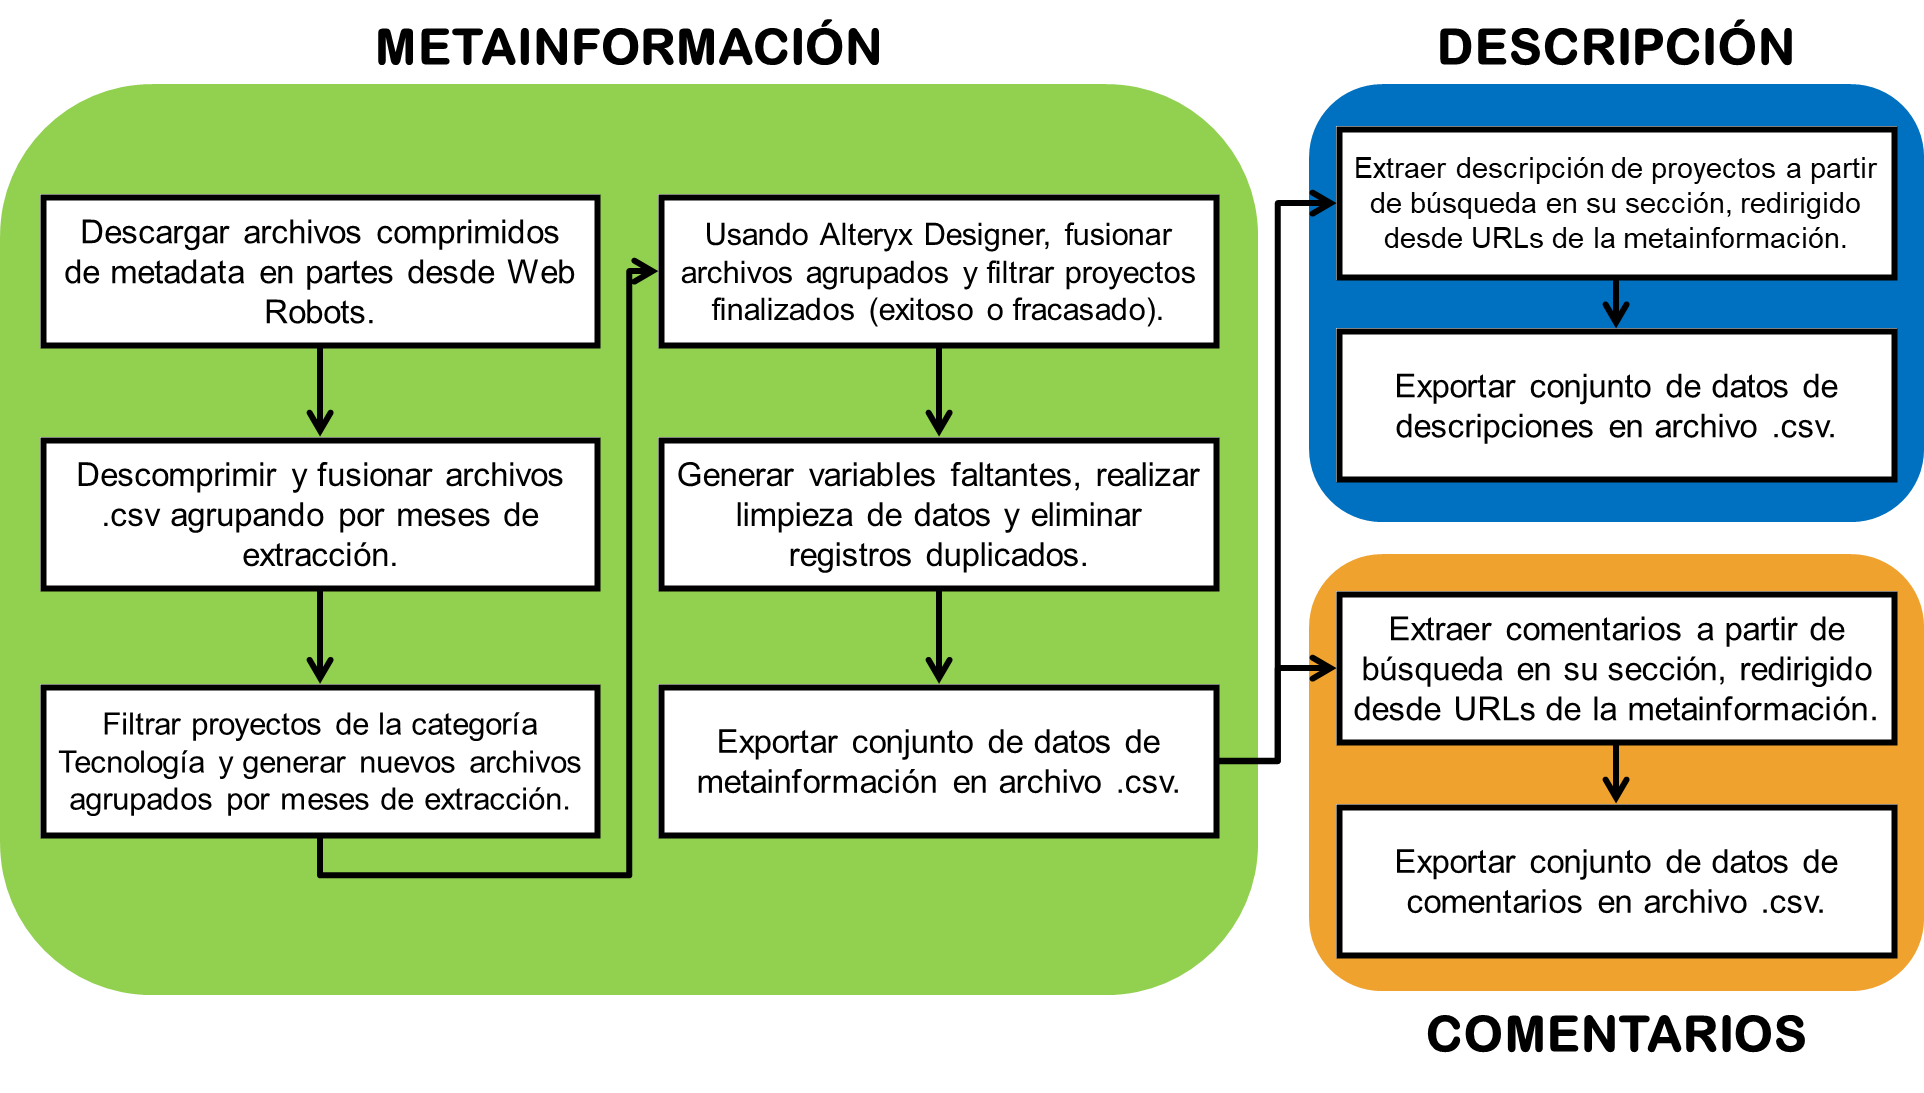
\includegraphics[width=0.89\textwidth]{3/figures/data_recolection_flux.png}
		\caption[Flujograma de la recolección de conjuntos finales de datos]{Flujograma de la recolección de conjuntos finales de datos.\\
			Fuente: Elaboración propia.}
		\label{3:fig1}
	\end{center}
\end{figure}

Asimismo, para encontrar algunos de los papers con la información requerida más cercana, se utilizaron keywords o palabras clave como \textit{crowdfunding}, \textit{Machine Learning}, \textit{Deep Learning}, \textit{prediction}, \textit{Kickstarter}, \textit{accuracy} y \textit{projects}.

%\newpage
\section{Técnicas para el procesamiento y análisis de la información}

\subsection{Metodología de implementación de la solución}
Como se explicó en el punto 2.2.6 del Marco Teórico del presente trabajo, según \cite{tec_braulio2015metodologiasdm}, dentro de los sistemas de analítica de negocio, Big Data y Minería de Datos, tres de las metodologías más usadas son CRISP-DM, SEMMA y KDD. Los mismos autores detallan en la Tabla \ref{2:table1} las características que cada una presenta al compararse.

Para escoger la metodología, se elaboró la Tabla \ref{3:table2} con el fin de comparar las utilizadas por los autores en los antecedentes. 17 de los 18 autores implementaron sus propias metodologías, las cuales de acuerdo a su similitud se agruparon en 8 grupos.

%\newpage
%\begin{table}[htbp]
\vspace{2ex}
\begingroup
	\renewcommand\arraystretch{0.2}
	\begin{longtable}{M{3cm}M{2.5cm}M{2.5cm}M{6cm}}
		\caption[Cuadro comparativo para la selección de la metodología]{Cuadro comparativo para la selección de la metodología.}
		\label{3:table2}
		\newcommand{\multirot}[1]{\multirow{2}{*}[-8ex]{\rotcell{\rlap{#1}}}}
		%\scriptsize
		\footnotesize
		\centering
		\small
		%% Se agrega tabularnewline para longtable
		\tabularnewline \specialrule{.1em}{.05em}{.05em}
		Metodología & Cantidad de referencias & Número de pasos & Nombre de los pasos
		\\
		\specialrule{.1em}{.05em}{.05em}
		{CRISP-DM}
		& 1
		& 6
		& \setlist{nolistsep}
		\begin{itemize}[label={--},nosep,noitemsep,leftmargin=*,topsep=0pt,partopsep=0pt]
			\item Comprensión del negocio.
			\item Comprensión de los datos.
			\item Preparación de los datos.
			\item Modelado.
			\item Evaluación.
			\item Despliegue.
		\end{itemize}                                                 
		\\
		\hline
		{Grupo A}
		& 2
		& 6
		& \setlist{nolistsep}
		\begin{itemize}[label={--},nosep,noitemsep,leftmargin=*,topsep=0pt,partopsep=0pt]
			\item Formulación del problema.
			\item Recolección de datos.
			\item Pre-procesamiento de datos.
			\item Modelado.
			\item Evaluación.
			\item Despliegue.
		\end{itemize} 
		\\
		\hline
		{Grupo B}
		& 1
		& 6
		& \setlist{nolistsep}
		\begin{itemize}[label={--},nosep,noitemsep,leftmargin=*,topsep=0pt,partopsep=0pt]
			\item Formulación del problema.
			\item Recolección de datos.
			\item Selección de características.
			\item Modelado.
			\item Evaluación.
			\item Despliegue.
		\end{itemize} 
		\\
		\hline
		{Grupo C}
		& 2
		& 5
		& \setlist{nolistsep}
		\begin{itemize}[label={--},nosep,noitemsep,leftmargin=*,topsep=0pt,partopsep=0pt]
			\item Recolección de datos.
			\item Pre-procesamiento de datos.
			\item Selección de características.
			\item Modelado.
			\item Evaluación.
		\end{itemize} 
		\\
		\hline
		{Grupo D}
		& 3
		& 5
		& \setlist{nolistsep}
		\begin{itemize}[label={--},nosep,noitemsep,leftmargin=*,topsep=0pt,partopsep=0pt]
			\item Formulación del problema.
			\item Recolección de datos.
			\item Pre-procesamiento de datos.
			\item Modelado.
			\item Evaluación.
		\end{itemize} 
		\\
		\hline
		{Grupo E}
		& 3
		& 5
		& \setlist{nolistsep}
		\begin{itemize}[label={--},nosep,noitemsep,leftmargin=*,topsep=0pt,partopsep=0pt]
			\item Recolección de datos.
			\item Pre-procesamiento de datos.
			\item Modelado.
			\item Evaluación.
			\item Despliegue.
		\end{itemize} 
		\\
		\hline
		{Grupo F}
		& 3
		& 4
		& \setlist{nolistsep}
		\begin{itemize}[label={--},nosep,noitemsep,leftmargin=*,topsep=0pt,partopsep=0pt]
			\item Recolección de datos.
			\item Pre-procesamiento de datos.
			\item Modelado.
			\item Evaluación.
		\end{itemize} 
		\\
		\hline
		{Grupo G}
		& 1
		& 4
		& \setlist{nolistsep}
		\begin{itemize}[label={--},nosep,noitemsep,leftmargin=*,topsep=0pt,partopsep=0pt]
			\item Recolección de datos.
			\item Modelado.
			\item Evaluación.
			\item Despliegue.
		\end{itemize} 
		\\
		\hline
		{Grupo H}
		& 2
		& 3
		& \setlist{nolistsep}
		\begin{itemize}[label={--},nosep,noitemsep,leftmargin=*,topsep=0pt,partopsep=0pt]
			\item Recolección de datos.
			\item Modelado.
			\item Evaluación.
		\end{itemize} 
		\\
		\specialrule{.1em}{.05em}{.05em}
	\end{longtable}%
\endgroup
	%\par	%%Salto de linea
	%\bigskip
	\begin{flushleft}	%%Alinear a la izquierda sin justificar
		\small Fuente: Elaboración propia
	\end{flushleft}
%\end{table}

Si bien es cierto que de las 3 metodologías mencionadas por \citeauthor{tec_braulio2015metodologiasdm}, solamente 1 autor especifica en su investigación el uso de una de ellas, en este caso CRISP-DM \parencite{pr_fernandezblanco2020crowdfunding_empirical}, otros 3 autores (grupos A y B) en sus propias metodologías siguieron secuencias de actividades que se encuentran comprendidas también dentro de esta metodología. Por su parte, los grupos C, F y H guardan cierta relación de semejanza con la metodología SEMMA por comprender enfocarse más en el modeloado, así como tener de primera actividad el Muestreo y culminar con la evaluación de resultados, obviando la actividad de formulación del problema. En el Anexo \ref{anexo4} se puede observar con más detalle las metodologías de la Tabla \ref{3:table2} asignadas a la investigación correspondiente.

Además de lo anterior expuesto, algunas de las siguientes características de acuerdo a la literatura también influyeron en la elección de la metodología CRISP-DM:

\begin{itemize}
	\item La metodología seleccionada contempla entre sus fases la comprensión del negocio además de la parte técnica que incluye el modelado y análisis de resultados. Esta guarda un rol importante ya que en ella se define el inicio de todo el proceso para dar el alcance del proyecto y definir objetivos que se buscan a partir de la Minería de Datos y Big Data. La formulación del problema se encuentra presente en el actual trabajo.
	\item Ayuda a los responsables del proyecto y/o investigación en la planeación y toma de decisiones (fase Despliegue) a partir de los resultados obtenidos, reportando y convirtiéndolos en oportunidades a considerar en los objetivos.
	\item Evalúa en todo el proceso los datos y variables usadas con el fin de crear el mejor modelo. Estas serán importantes para interpretar los resultados y tomar decisiones.
	\item Respecto a las otras dos metodologías, ambas omiten en su primera iteración la formulación del problema, la cual se encuentra presente en el actual trabajo. Por el lado de KDD, si bien esta contempla 9 pasos durante su proceso, el objetivo de KDD en cada uno de estos resulta ser más técnico, es decir, trabajar, seleccionar e interpretar métricas, variables, modelos, entre otros para obtener los mejores resultados más allá de considerar el contexto y comprensión del negocio. De hecho, no existe alguna fase dedicada al entendimiento del mismo.
	\item Por otra parte, la metodología SEMMA se basa, como su nombre lo indica, en la selección, exploración y modelado de grandes cantidades de datos para descubrir patrones de negocio desconocidos. Sin embargo, al limitarse a 5 fases comenzando con la fase de muestreo, no hace hincapié en la comprensión del negocio, sino más bien comienza con el procesamiento de datos para la construcción del modelo.
\end{itemize}

Cada una de las fases de la metodología seleccionada se detalla en la Figura \ref{3:fig2}.

\begin{figure}[htbp]
	\begin{center}
		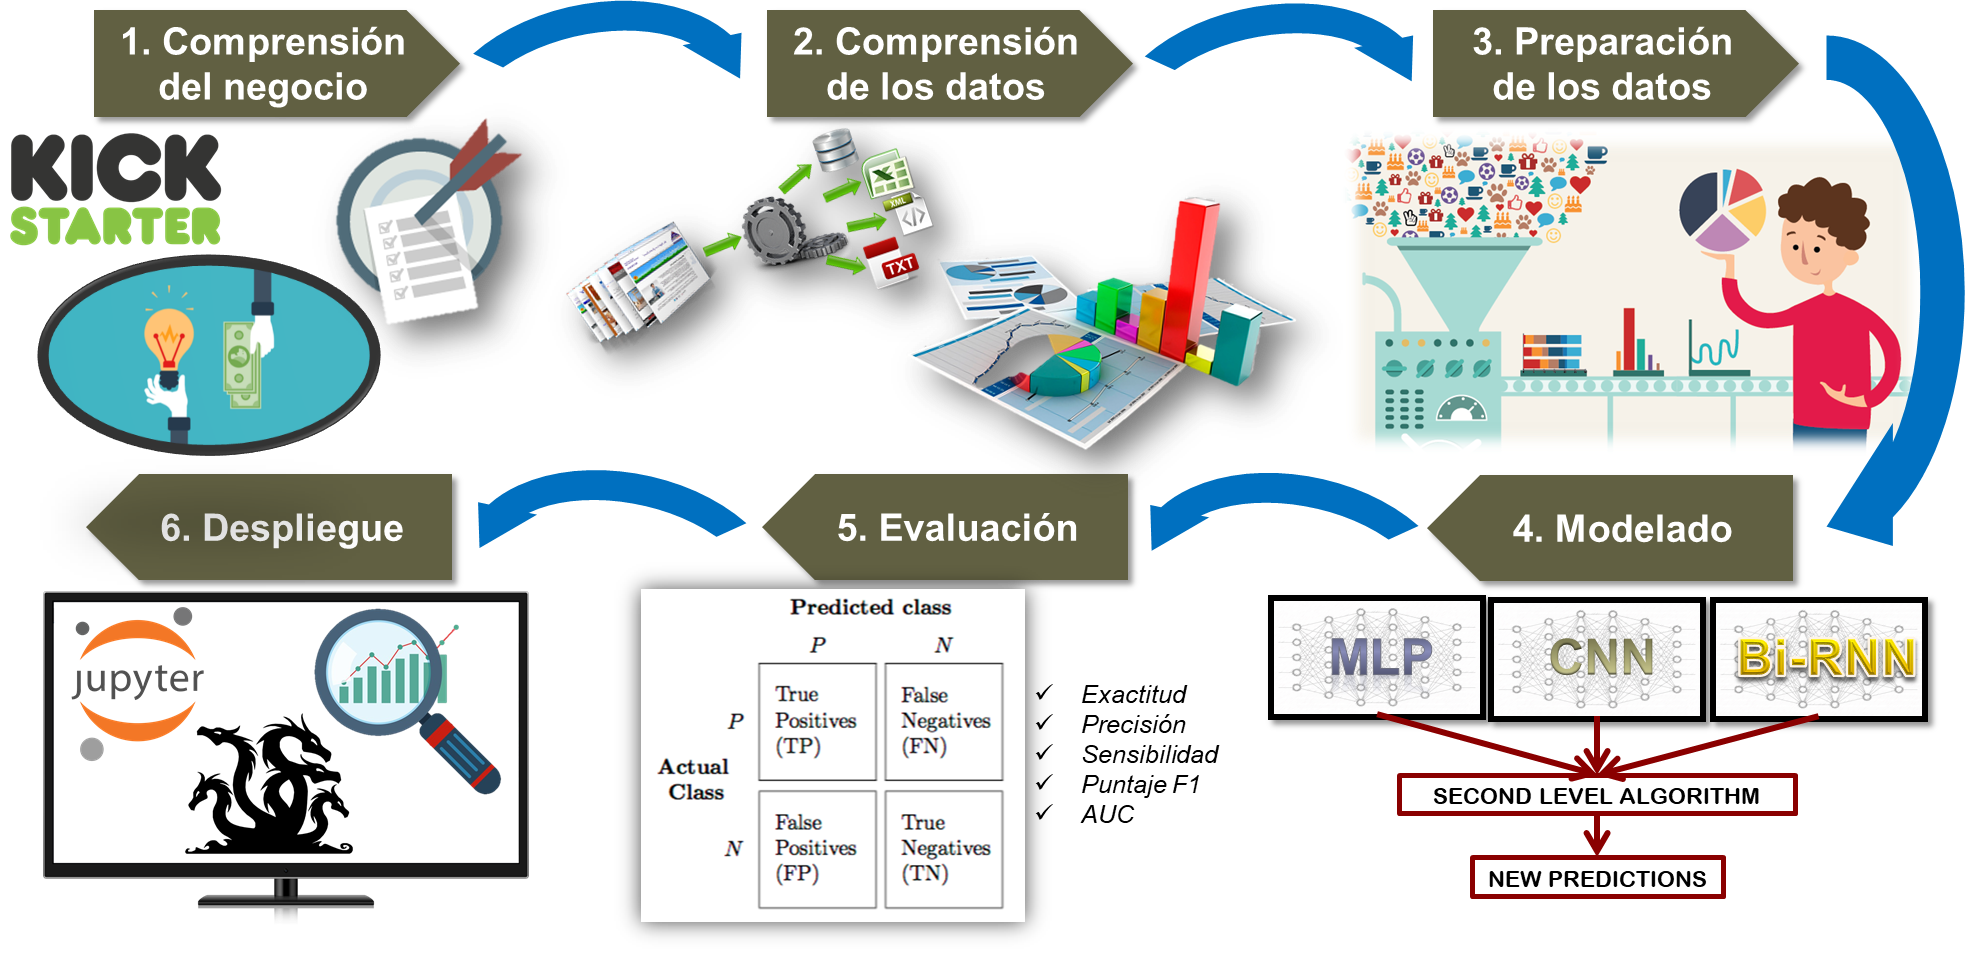
\includegraphics[width=1\textwidth]{3/figures/metodologia.png}
		\caption[Metodología de la investigación]{Metodología de la investigación.\\
			Fuente: Elaboración propia}
		\label{3:fig2}
	\end{center}
\end{figure}

Durante el proceso de la implementación de la metodología, en donde se decidió construir un modelo de Aprendizaje Profundo Multimodal (utilizado por \cite{pr_kamath2018suplearn}, \cite{pr_jin2019dayssuccess}, y \cite{pr_cheng2019deeplearning}), de acuerdo a la literatura, se analizaron las siguientes posibles modalidades que se tomarían en cuenta para la investigación:

\begin{itemize}
	\item \textbf{Metainformación}: \cite{pr_chen2013kickpredict}, \cite{pr_mitra2014phrases}, \cite{pr_zhou2015projectdesc}, \cite{pr_chen2015predcrowd}, \cite{pr_beckwith2016predcrowd}, \cite{pr_li2016predcrowd}, \cite{pr_yuan2016textanalytics}, \cite{pr_sawhney2016usingLT}, \cite{pr_kaur2017socmedcrowd}, \cite{pr_kamath2018suplearn}, \cite{pr_yu2018deeplearning}, \cite{pr_jin2019dayssuccess}, \cite{pr_cheng2019deeplearning}, \cite{pr_fernandezblanco2020crowdfunding_empirical}.
	\item \textbf{Descripción del proyecto}: \cite{pr_mitra2014phrases}, \cite{pr_zhou2015projectdesc}, \cite{pr_yuan2016textanalytics}, \cite{pr_sawhney2016usingLT}, \cite{pr_kamath2018suplearn}, \cite{pr_lee2018contentDL}, \cite{pr_jin2019dayssuccess}, \cite{pr_cheng2019deeplearning}, \cite{pr_chen2019keywords_crowdfunding}, \cite{pr_chaichi2019nlp_3dprinting}.
	\item \textbf{Comentarios en la campaña}: \cite{pr_chen2015predcrowd}, \cite{pr_li2016predcrowd}, \cite{pr_lee2018contentDL}, \cite{pr_jin2019dayssuccess}, \cite{pr_shafqat2019topicpredictions}.
	\item \textbf{Actualizaciones y/o recompensas}: \cite{pr_zhou2015projectdesc}, \cite{pr_lee2018contentDL}.
	\item \textbf{Contenido audiovisual (imagen y/o video del proyecto)}: \cite{pr_cheng2019deeplearning}.
\end{itemize}

De las anteriores modalidades, las actualizaciones no representan un cambio significativo ya que consisten en agregar o desagregar contenido textual o modificar recompensas en la campaña. Por el lado del contenido audiovisual, además de no presentarse en todas las campañas, para el caso particular de la categoría Tecnología no se encontró un patrón entre sus imágenes que pueda ser de utilidad, como se presenta en el trabajo de tesis de pregrado del presente investigador \parencite{pr_puente2019kickstarter_prediction}.

Finalmente, fueron seleccionadas las modalidades de metainformación, descripción del proyecto y comentarios, para este último considerando solamente expresados por patrocinadores. Las 2 primeras se localizan en la sección principal de la campaña, mientras que la tercera se ubica en su sección respectiva, como se puede apreciar en la Figura \ref{3:fig3}.
\begin{figure}[htbp]
	\begin{center}
		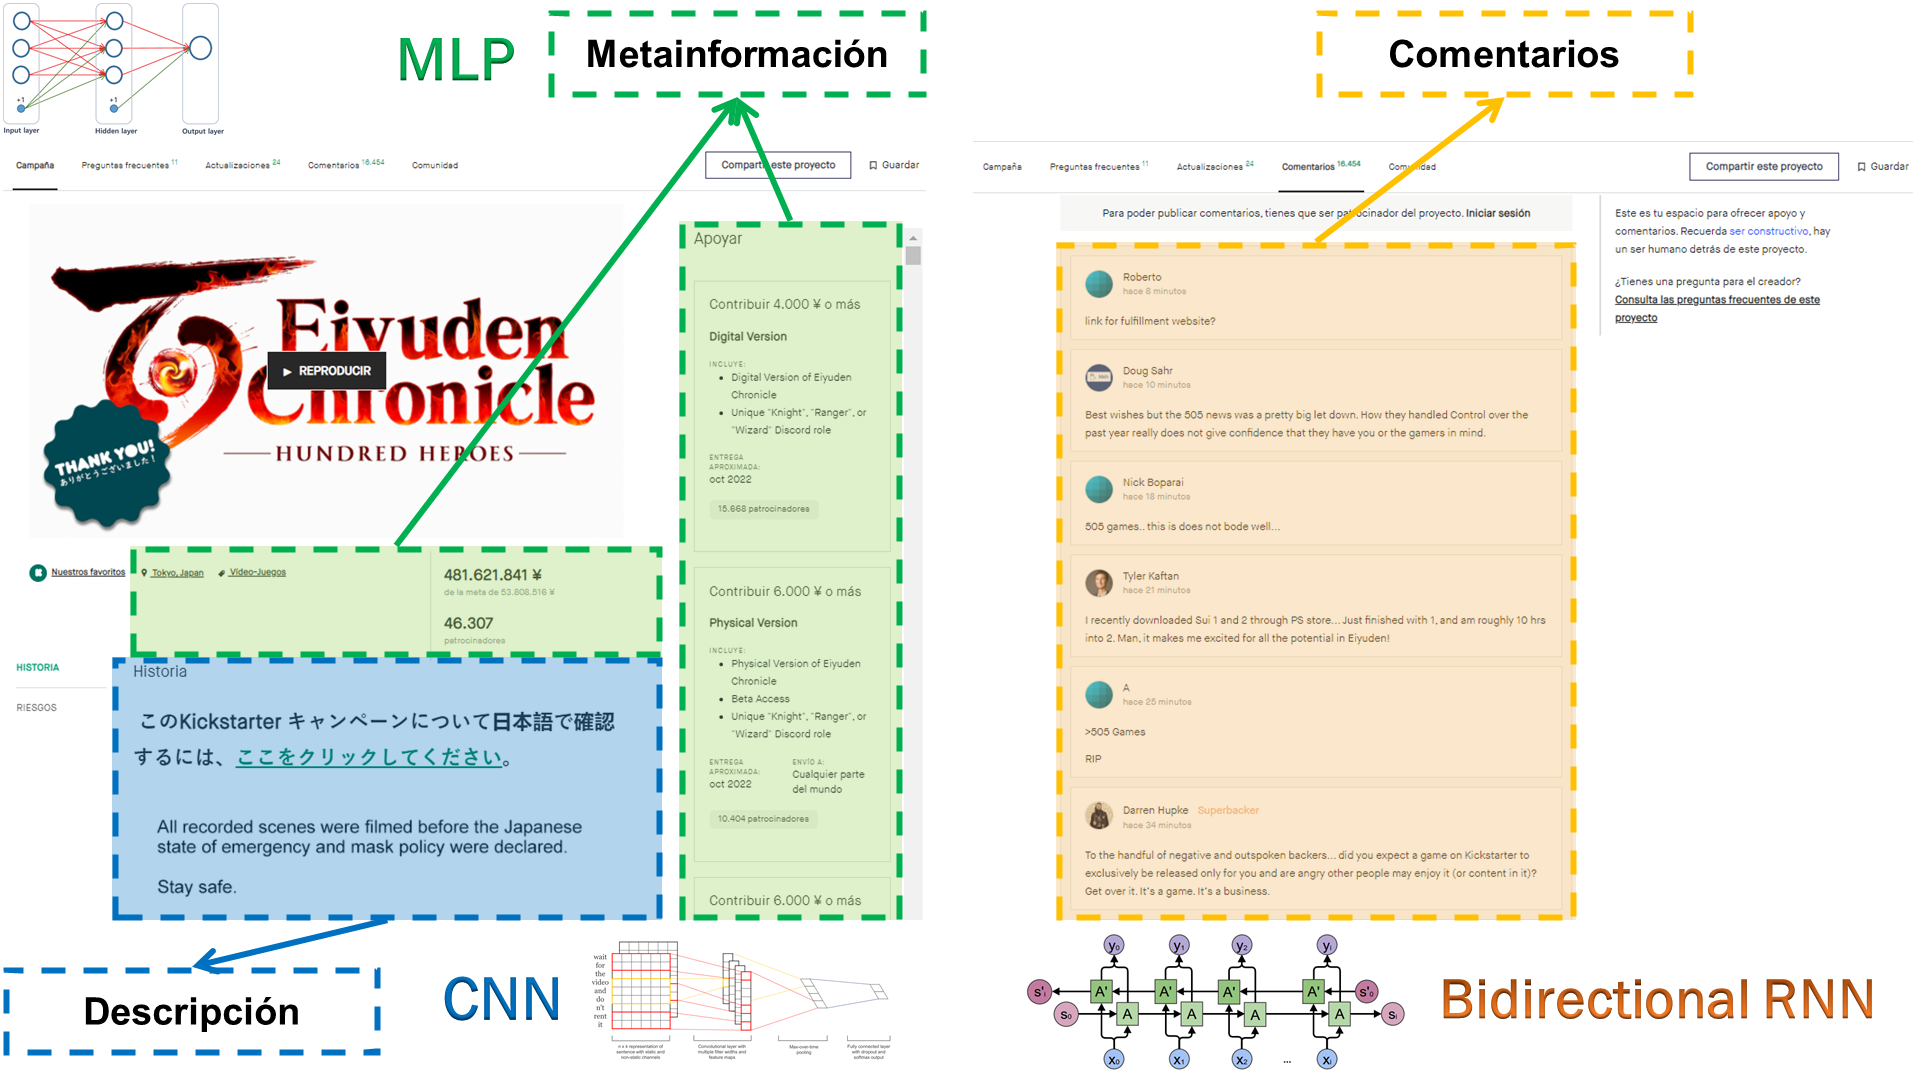
\includegraphics[width=0.90\textwidth]{3/figures/framework.png}
		\caption[Marco de trabajo del prototipo final]{Marco de trabajo del prototipo final.\\
			Fuente: Elaboración propia}
		\label{3:fig3}
	\end{center}
\end{figure}

\newpage
\subsubsection{Comprensión del negocio}
En la primera fase, se definió el problema a partir de comprender el contexto de la investigación. A partir de aquí, se formularon los objetivos y requerimientos que se espera lograr en el proyecto. La lista de actividades y tareas se presenta en la Tabla \ref{3:table3}.

\vspace{2ex}
\begingroup
\renewcommand\arraystretch{0.3}
\begin{longtable}{m{5cm}m{5cm}M{5cm}}
	\caption[Actividades de fase Comprensión del negocio]{Actividades de fase Comprensión del negocio.}
	\label{3:table3}
	\newcommand{\multirot}[1]{\multirow{2}{*}[-8ex]{\rotcell{\rlap{#1}}}}
	%\scriptsize
	\footnotesize
	%\centering
	\small
	%% Se agrega tabularnewline para longtable
	\tabularnewline \specialrule{.1em}{.05em}{.05em}
	\centering Actividades & \centering Descripción & Tareas
	\\
	\specialrule{.1em}{.05em}{.05em}
	Definir problemas, objetivos e hipótesis.
	& Definición de los problemas, objetivos e hipótesis generales y específicos de la investigación.
	& \setlist{nolistsep}
	\begin{itemize}[label={--},nosep,noitemsep,leftmargin=*,topsep=0pt,partopsep=0pt]
		\item Identificar la realidad problemática del contexto.
		\item Definir los objetivos de la investigación.
		\item Formular las hipótesis del trabajo.
	\end{itemize}                                               
	\\
	\hline
	Desarrollar la literatura de la investigación.
	& Selección de los antecedentes y trabajos previos relacionados a la investigación.
	& \setlist{nolistsep}
	\begin{itemize}[label={--},nosep,noitemsep,leftmargin=*,topsep=0pt,partopsep=0pt]
		\item Buscar material académico sobre las variables de la investigación.
		\item Buscar material académico relacionado a la solución de la realidad problemática.
	\end{itemize} 
	\\
	\hline
	Definir metodología de la investigación.
	& Definición de la metodología a implementarse en el estudio.
	& \setlist{nolistsep}
	\begin{itemize}[label={--},nosep,noitemsep,leftmargin=*,topsep=0pt,partopsep=0pt]
		\item Evaluar metodologías de la literatura.
		\item Seleccionar metodología a implementar en el trabajo.
	\end{itemize} 
	\\
	\specialrule{.1em}{.05em}{.05em}
\end{longtable}%
\endgroup

%\par	%%Salto de linea
%\bigskip
\begin{flushleft}	%%Alinear a la izquierda sin justificar
	\small Fuente: Elaboración propia
\end{flushleft}

A continuación, cada actividad de la anterior tabla es detallada y se indican sus entregables respectivos.

\newpage
\textbf{Actividad 1: Definir problemas, objetivos e hipótesis}
\\
En esta actividad se detalla cómo se definieron los problemas, objetivos e hipótesis generales y específicos de la investigación a partir del estudio de la coyuntura en que se desenvuelve la realidad problemática.

\textbf{Entregable}: Problemas, objetivos e hipótesis definidos.


\textbf{Actividad 2: Desarrollar la literatura de la investigación}
\\
A partir de la definición de los objetivos, se realizó la búsqueda de fuentes, publicaciones, libros, artículos y material académico relacionado al contexto del financiamiento colectivo, sus características y qué métodos se utilizaron para resolver problemas dentro del entorno. Asimismo, se elaboró el marco teórico abordado en el estudio.

\textbf{Entregable}: Material académico y conocimientos obtenidos sobre el ambiente del crowdfunding y la Inteligencia Artificial.


\textbf{Actividad 3: Definir metodología de la investigación}
\\
Luego de conseguir los recursos intelectuales suficientes y los trabajos previos para el desarrollo de la investigación, se analizó cada antecedente y se compararon todas las metodologías implementadas por cada autor. Al culminar con esta tarea, en base a la literatura y los procesos más alineados al presente trabajo, se seleccionó la metodología CRISP-DM como la mejor opción.

\textbf{Entregable}: Metodología de implementación de la solución.


\subsubsection{Comprensión de los datos}
La segunda fase abarcó tanto la recolección de los datos como el análisis estadístico de estos para conocer un poco más sus características. El conjunto total de datos utilizado para la investigación consistió en la recolección de 27,251 proyectos tecnológicos de Kickstarter comprendidos entre los años 2009 y 2019, en 3 partes: metainformación, descripción y comentarios (excluyendo los del creador) del proyectos.

Para ello, se elaboró una lista de actividades y tareas presentadas en la Tabla \ref{3:table4}.

\vspace{2ex}
\begingroup
\renewcommand\arraystretch{0.3}
\begin{longtable}{m{4cm}m{5.5cm}M{5.5cm}}
	\caption[Actividades de fase Comprensión de los datos]{Actividades de fase Comprensión de los datos.}
	\label{3:table4}
	\newcommand{\multirot}[1]{\multirow{2}{*}[-8ex]{\rotcell{\rlap{#1}}}}
	%\scriptsize
	\footnotesize
	%\centering
	\small
	%% Se agrega tabularnewline para longtable
	\tabularnewline \specialrule{.1em}{.05em}{.05em}
	\centering Actividades & \centering Descripción & Tareas
	\\
	\specialrule{.1em}{.05em}{.05em}
	Construir base de datos de Metainformación.
	& Construcción de base de datos que contenga las variables de la campaña con excepción del contenido textual (descripción, actualizaciones y comentarios acerca del proyecto).
	& \setlist{nolistsep}
	\begin{itemize}[label={--},nosep,noitemsep,leftmargin=*,topsep=0pt,partopsep=0pt]
		\item Descargar conjuntos de datos comprimidos de la página Web Robots.
		\item Descomprimir archivos en partes y fusionarlos en uno solo según su mes.
		\item Fusionar archivos por mes, realizar limpieza de datos y generar base final.
	\end{itemize} 
	\\
	\hline
	Construir base de datos de Descripción.
	& Construcción de base de datos que contenga la descripción del proyecto en la página principal de la campaña.
	& \setlist{nolistsep}
	\begin{itemize}[label={--},nosep,noitemsep,leftmargin=*,topsep=0pt,partopsep=0pt]
		\item Identificar sección de descripción a partir de la búsqueda del URL desde la base de datos de Metainformación.
		\item Capturar información de sección identificada.
		\item Generar base final.
	\end{itemize} 
	\\
	\hline
	Construir base de datos de Comentarios.
	& Construcción de base de datos que contenga los comentarios de los patrocinadores del proyecto en su sección correspondiente.
	& \setlist{nolistsep}
	\begin{itemize}[label={--},nosep,noitemsep,leftmargin=*,topsep=0pt,partopsep=0pt]
		\item Identificar sección de comentarios a partir de la búsqueda del URL desde la base de datos de Metainformación.
		\item Capturar información de sección identificada, excluyendo comentarios y respuestas de los creadores del proyecto.
		\item Generar base final.
	\end{itemize}
	\\
	\hline
	Realizar análisis exploratorio y estadístico de variables considerados.
	& Análisis exploratorio y estadístico de las variables disponibles para cada modalidad.
	& \setlist{nolistsep}
	\begin{itemize}[label={--},nosep,noitemsep,leftmargin=*,topsep=0pt,partopsep=0pt]
		\item Describir distribución de los datos y tendencias.
		\item Analizar existencia de correlación entre variables.
	\end{itemize}
	\\
	\specialrule{.1em}{.05em}{.05em}
\end{longtable}%
\endgroup

%\par	%%Salto de linea
%\bigskip
\begin{flushleft}	%%Alinear a la izquierda sin justificar
	\small Fuente: Elaboración propia
\end{flushleft}

A continuación, se detalla cada actividad y su entregable respectivo.

\textbf{Actividad 1: Construir base de datos de Metainformación}
\\
De acuerdo a la Figura \ref{3:fig1}, en esta actividad se enfocó en la construcción de la base de datos de la Metainformación desde la descarga de los conjuntos de datos comprimidos de la página Web Robots hasta la generación del archivo final luego de limpiar los datos.

La 2 primeras tareas de la anterior tabla se resumen en el flujo de la Figura \ref{3:fig4}.

\begin{figure}[h]
	\begin{center}
		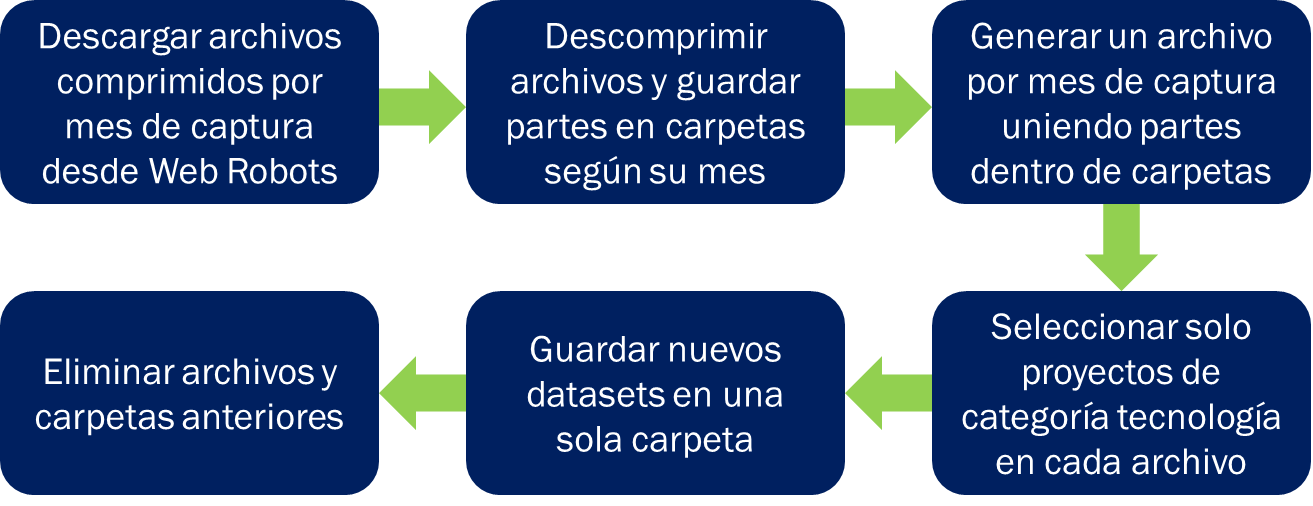
\includegraphics[width=0.8\textwidth]{3/figures/flujograma_metadata_t1_t2.png}
		\caption[Proceso de obtención y preparación de datasets iniciales de Metainformación]{Proceso de obtención y preparación de datasets iniciales de Metainformación.\\
			Fuente: Elaboración propia.}
		\label{3:fig4}
	\end{center}
\end{figure}

La siguiente fase de la actividad fue la selección de variables y limpieza de datos utilizando el software Alteryx Designer, el cual permite desarrollar flujos de trabajo para preparar, unir y analizar volúmenes de datos complejos de distintas fuentes. Se ejecutó el flujograma representado de forma resumida en la Figura \ref{3:fig5}.

\begin{figure}[h]
	\begin{center}
		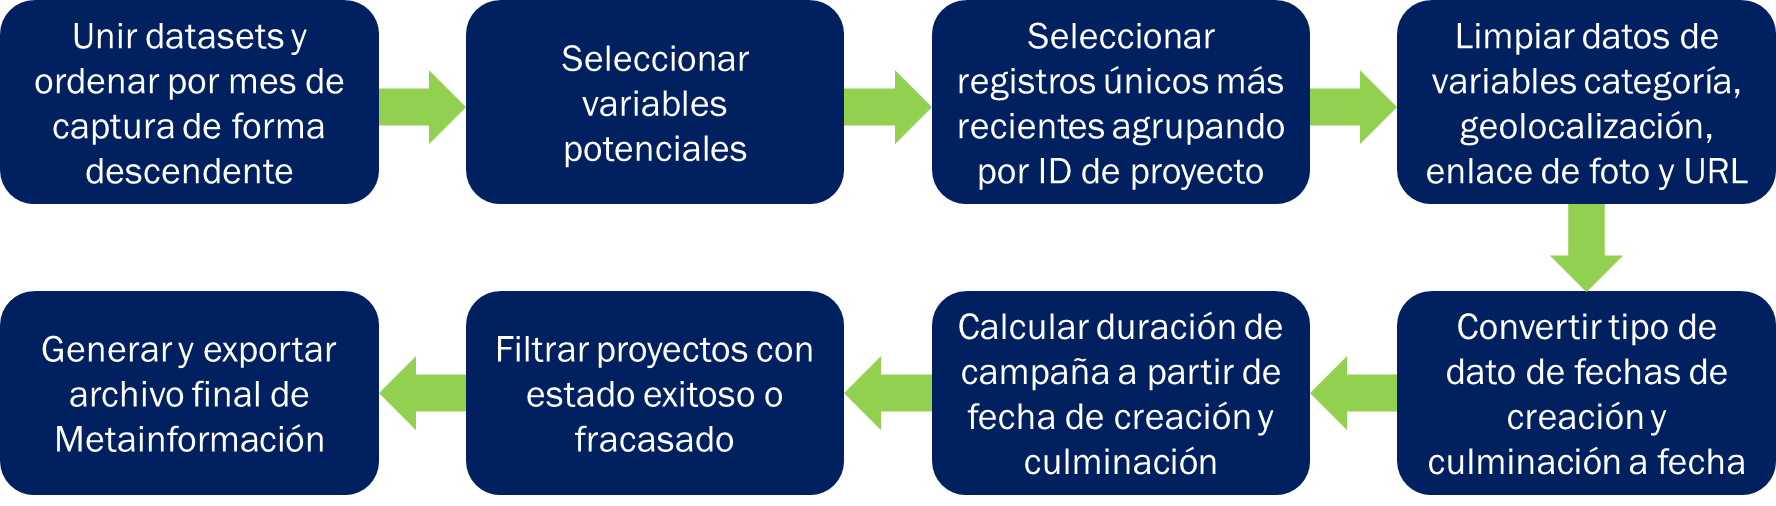
\includegraphics[width=1\textwidth,clip]{3/figures/flujograma_metadata_t3.png}
		\caption[Proceso resumido de generación de conjunto final de Metainformación]{Proceso resumido de generación de conjunto final de Metainformación.\\
			Fuente: Elaboración propia.}
		\label{3:fig5}
	\end{center}
\end{figure}

\textbf{Entregable}: Conjunto de datos de Metainformación, que contiene 19 variables cuantitativas y cualitativas para la muestra considerada.

\textbf{Actividad 2: Construir base de datos de Descripción}
\\
De acuerdo a la Figura \ref{3:fig1}, una vez generado el conjunto de datos de Metainformación descrito en la anterior actividad, a partir de la variable \textit{urls} se puede extraer la descripción de cada proyecto, siguiendo el proceso del diagrama de flujo representado en la Figura \ref{3:fig6}.

\begin{figure}[h]
	\begin{center}
		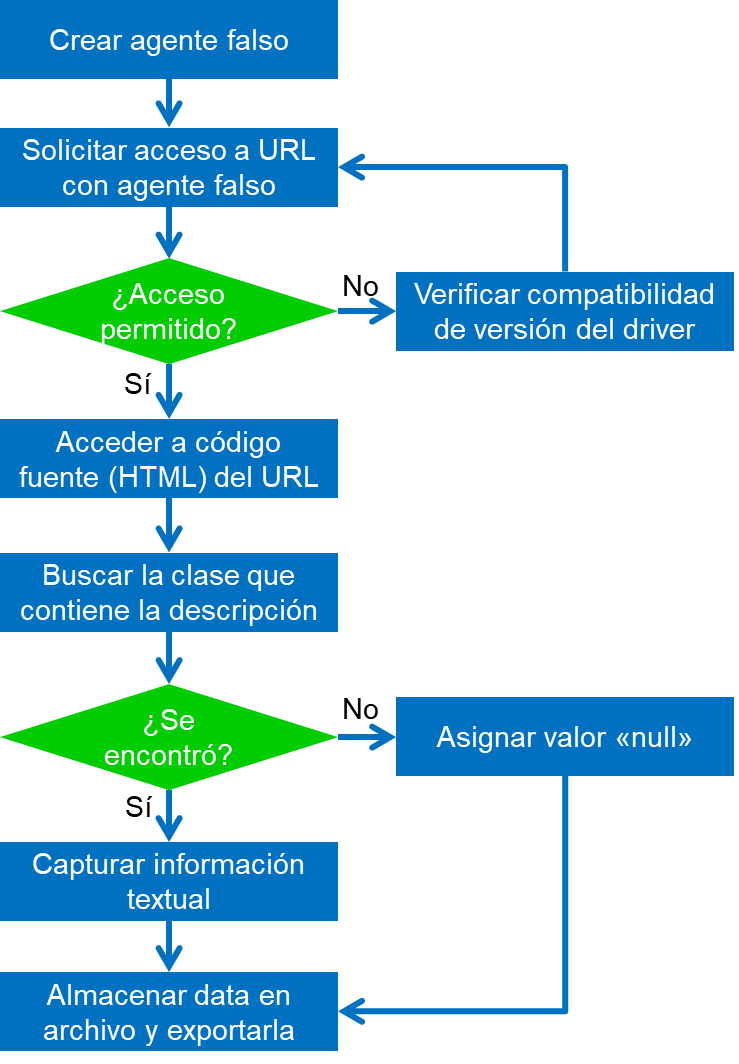
\includegraphics[width=0.5\textwidth]{3/figures/diagrama_flujo_scrapping_descripcion.png}
		\caption[Proceso de extracción de la descripción de un proyecto]{Proceso de extracción de la descripción de un proyecto.\\
			Fuente: Elaboración propia.}
		\label{3:fig6}
	\end{center}
\end{figure}

\textbf{Entregable}: Conjunto de datos de Descripción, que contiene la variable textual de descripción del proyecto para la muestra considerada.

\textbf{Actividad 3: Construir base de datos de Comentarios}
\\
De acuerdo a la Figura \ref{3:fig1}, y realizando el mismo ejercicio con Descripción, una vez generado el conjunto de datos de Metainformación, a partir de la variable \textit{urls} se pueden extraer los comentarios de los patrocinadores por cada proyecto, siguiendo el proceso del diagrama de flujo representado en la Figura \ref{3:fig7}.

\begin{figure}[h]
	\begin{center}
		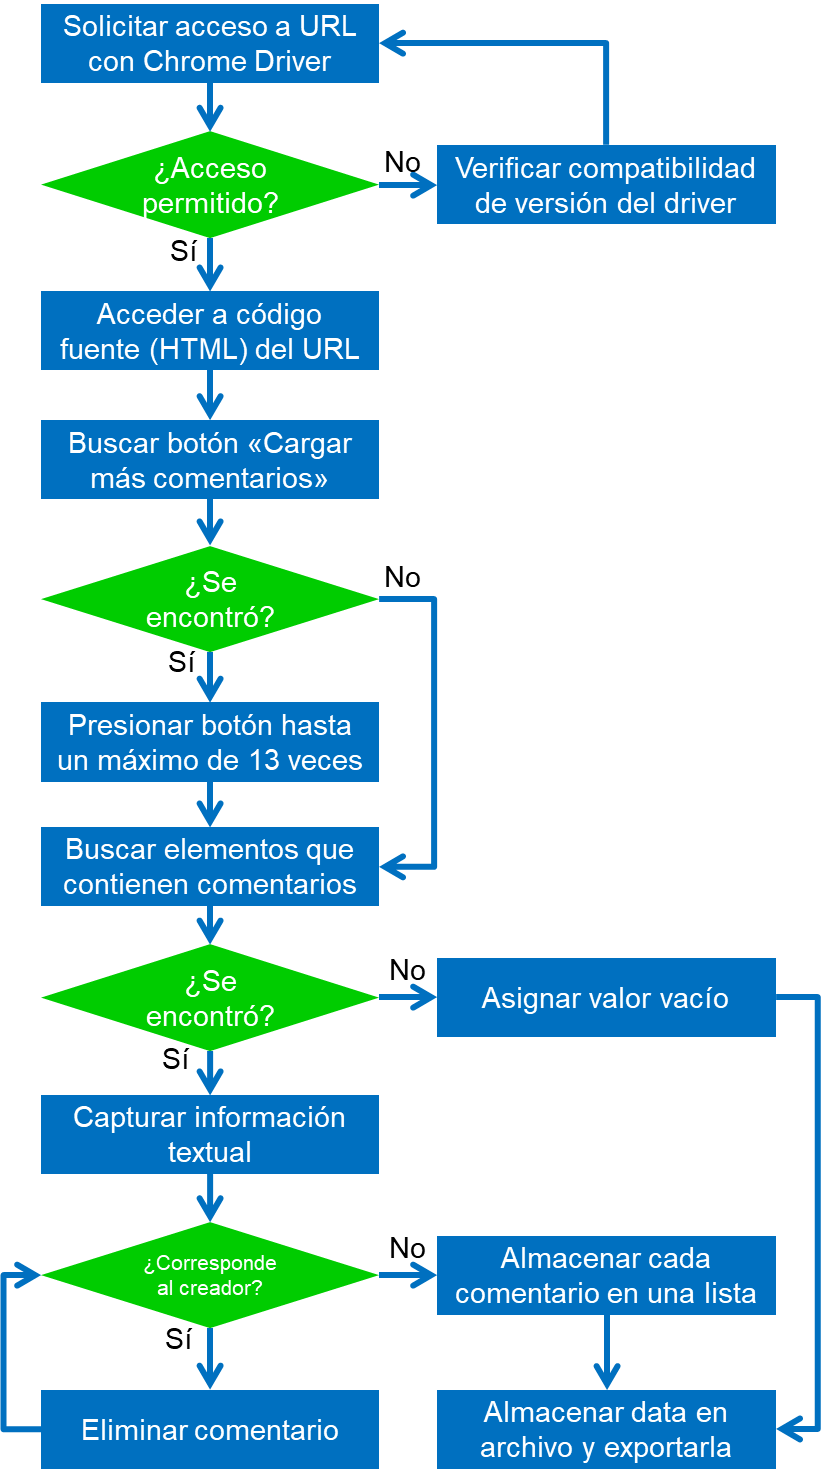
\includegraphics[width=0.45\textwidth]{3/figures/diagrama_flujo_scrapping_comentarios.png}
		\caption[Proceso de extracción de comentarios de un proyecto]{Proceso de extracción de comentarios de un proyecto.\\
			Fuente: Elaboración propia.}
		\label{3:fig7}
	\end{center}
\end{figure}

\textbf{Entregable}: Conjunto de datos de Comentarios, que contiene la variable textual de comentarios de los patrocinadores, cada uno separado por autor y almacenados en conjunto en una lista por proyecto, para la muestra considerada.

\textbf{Actividad 4: Realizar análisis exploratorio y estadístico de variables considerados}
\\
En esta actividad, las variables de los 3 conjuntos finales de datos se describen en distribución de gráficos de barras, diagramas de cajas y bigotes y análisis de correlaciones de variables para la Metainformación; y nubes de palabras para la Descripción y Comentarios.

\textbf{Entregable}: Gráficos estadísticos de Metainformación, Descripción y Comentarios.

\subsubsection{Preparación de los datos}
En el anterior paso, se logró analizar estadísticamente las tendencias y distribuciones de cada variable según su respectiva modalidad. En esta etapa, como se detalla en la Tabla \ref{3:table5}, las variables observadas fueron pre-procesadas con la finalidad de incluir datos homologados que no afecten negativamente el rendimiento de los modelos.

\vspace{2ex}
\begingroup
\renewcommand\arraystretch{0.3}
\begin{longtable}{m{5cm}m{5cm}M{5cm}}
	\caption[Actividades de fase Preparación de los datos]{Actividades de fase Preparación de los datos.}
	\label{3:table5}
	\newcommand{\multirot}[1]{\multirow{2}{*}[-8ex]{\rotcell{\rlap{#1}}}}
	%\scriptsize
	\footnotesize
	%\centering
	\small
	%% Se agrega tabularnewline para longtable
	\tabularnewline \specialrule{.1em}{.05em}{.05em}
	\centering Actividades & \centering Descripción & Tareas
	\\
	\specialrule{.1em}{.05em}{.05em}
	Pre-procesar base de datos de Metainformación.
	& Pre-procesamiento de las variables actuales y adicionales luego de evaluación de su comportamiento entre ellas.
	& \setlist{nolistsep}
	\begin{itemize}[label={--},nosep,noitemsep,leftmargin=*,topsep=0pt,partopsep=0pt]
		\item Añadir más variables cuantitativas según literatura.
		\item Evaluar comportamiento de variables en conjunto utilizando matriz de correlaciones.
		\item Armar grupos combinatorias potenciales de variables.
		\item Escalar variables a un mismo rango.
	\end{itemize}                                             
	\\
	\hline
	Pre-procesar base de datos de Descripción.
	& Pre-procesamiento de la variable \textit{description}.
	& \setlist{nolistsep}
	\begin{itemize}[label={--},nosep,noitemsep,leftmargin=*,topsep=0pt,partopsep=0pt]
		\item Realizar limpieza de datos de los textos.
		\item Armar vocabulario de palabras únicas.
		\item Transformar textos en vectores de palabras.
	\end{itemize} 
	\\
	\hline
	Pre-procesar base de datos de Comentarios.
	& Pre-procesamiento de la variable \textit{comments}.
	& \setlist{nolistsep}
	\begin{itemize}[label={--},nosep,noitemsep,leftmargin=*,topsep=0pt,partopsep=0pt]
		\item Realizar limpieza de datos de los textos.
		\item Armar vocabulario de palabras únicas.
		\item Transformar textos en vectores de palabras.
	\end{itemize}
	\\
	\specialrule{.1em}{.05em}{.05em}
\end{longtable}%
\endgroup

%\par	%%Salto de linea
%\bigskip
\begin{flushleft}	%%Alinear a la izquierda sin justificar
	\small Fuente: Elaboración propia
\end{flushleft}

A continuación, se detalla cada actividad y su entregable respectivo.

\textbf{Actividad 1: Pre-procesar base de datos de Metainformación}
\\
En esta actividad, antes de realizar el pre-procesamiento de las variables finales, se agregaron algunas cuantitativas sugeridas en la literatura que no estaban consideradas inicialmente. Para evaluar correctamente el nuevo conjunto de variables, se realizó un nuevo análisis de correlación y se armaron grupos de combinatorias de variables cuyos rendimientos serán medidos en los siguientes pasos. Previamente a la evaluación, los subconjuntos de entrenamiento y prueba divididos en 80\% y 20\% respectivamente (según \cite{pr_yuan2016textanalytics}, \cite{pr_yu2018deeplearning}, \cite{pr_chen2019keywords_crowdfunding}, \cite{pr_mitra2014phrases} y \cite{pr_sawhney2016usingLT}) estratificados según la variable \textit{state}, se escalaron a un mismo rango para evitar un entrenamiento incorrecto.

\textbf{Entregable}: Conjuntos de datos pre-procesados de Metainformación.

\textbf{Actividad 2: Pre-procesar base de datos de Descripción}
\\
Esta actividad se resume en la Figura \ref{3:fig8}, en donde se realizó desde la limpieza de los datos textuales, eliminando palabras y partes de ellas que no aportan para el diccionario final que se usará en la siguiente etapa, hasta la elaboración del vocabulario de palabras únicas, mayormente sustantivos y verbos en su forma original, los cuales se les asignaron un código para poder formar vectores de palabras y crear más adelante, las incrustaciones de palabras.

\begin{figure}[!ht]
	\begin{center}
		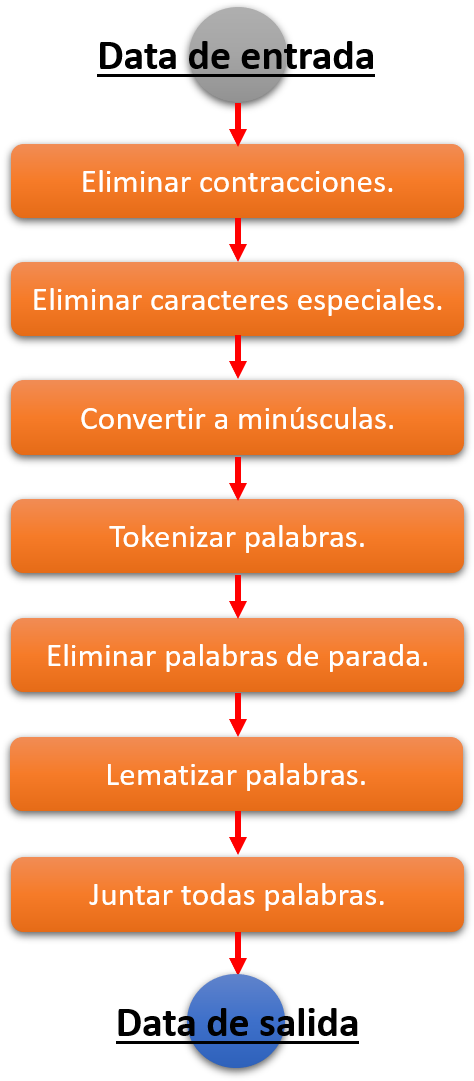
\includegraphics[width=0.33\textwidth]{3/figures/description_data_clean.png}
		\caption[Proceso de limpieza de conjunto de datos de descripciones]{Proceso de limpieza de conjunto de datos de descripciones.\\
			Fuente: Elaboración propia.}
		\label{3:fig8}
	\end{center}
\end{figure}

Luego de separar, al igual que la Metainformación, los subconjuntos de entrenamiento y prueba en 80\% y 20\% respectivamente estratificados según la variable \textit{state}, se ejecutó el proceso de la Figura \ref{3:fig9} dividido en 2 partes.

\begin{figure}[!ht]
	\centering
	\small
	\begin{subfigure}{.50\textwidth}
		\centering
		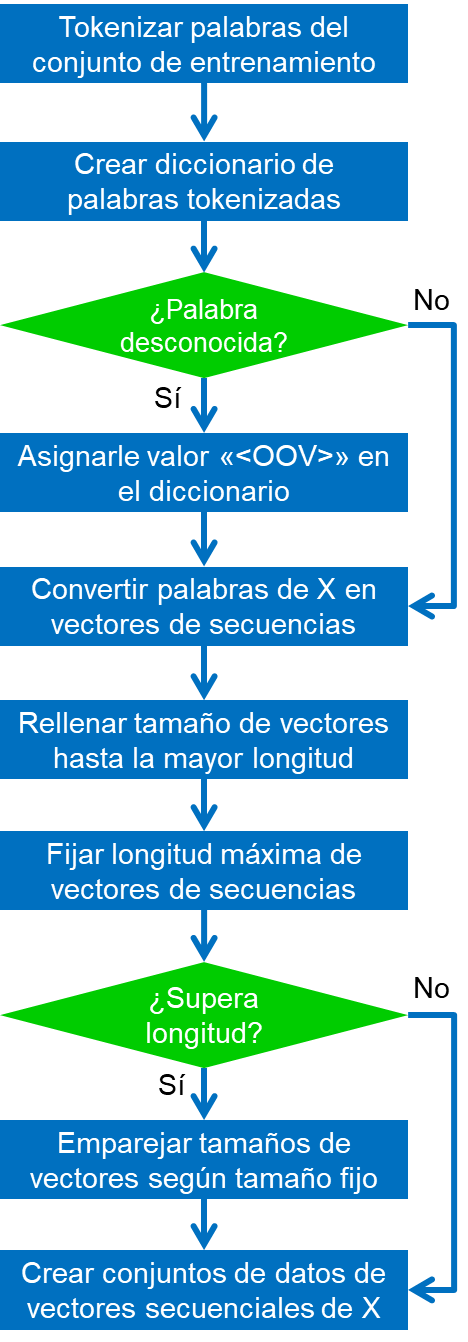
\includegraphics[width=0.65\linewidth]{3/figures/description_text_to_sequence.png}
		\caption{vectorización de palabras}
	\end{subfigure}%
	\begin{subfigure}{.50\textwidth}
		\centering
		\includegraphics[width=0.55\linewidth]{3/figures/description_embedding_matrix.png}
		\caption{matriz de incrustaciones de palabras}
	\end{subfigure}
	\caption[Procesos de vectorización y creación de matriz incrustaciones de palabras]{Procesos de vectorización y creación de matriz incrustaciones de palabras.\\
		Fuente: Elaboración propia.}
	\label{3:fig9}
\end{figure}

La primera mitad corresponde a la transformación del texto, para los subconjuntos de entrenamiento y prueba, de las descripciones en representaciones de vectores numéricos para la fase de entrenamiento del modelo. De forma paralela, se creó una matriz de incrustaciones de palabras que será parte de la capa de incrustaciones en la arquitectura del modelo.

\textbf{Entregable}: Descripciones representadas en secuencias de vectores numéricos y matriz de incrustaciones de palabras.

\textbf{Actividad 3: Pre-procesar base de datos de Comentarios}
\\
Al igual que en el proceso de Descripción, se realizó la limpieza de los datos textuales siguiendo la misma secuencia de la Figura \ref{3:fig7} para generar la representación de palabras de los comentarios en vectores numéricos, con la diferencia de acotar el tamaño final de los vectores debido a su extensa longitud al agruparse todos aquellos separados por autor. De igual manera, para generar la matriz de incrustaciones de palabras, se repitió el proceso de la Figura \ref{3:fig9}.

\textbf{Entregable}: Comentarios representadas en secuencias de vectores numéricos y matriz de incrustaciones de palabras.

\subsubsection{Modelamiento}
Al concluir la etapa del pre-procesamiento, las variables pudieron ser utilizadas para los modelos de cada modalidad, que fueron diseñados siguiendo las actividades de la Tabla \ref{3:table6}.

\vspace{2ex}
\begingroup
\renewcommand\arraystretch{0.3}
\begin{longtable}{m{4.6cm}m{4.9cm}M{5.5cm}}
	\caption[Actividades de fase Modelamiento]{Actividades de fase Modelamiento.}
	\label{3:table6}
	\newcommand{\multirot}[1]{\multirow{2}{*}[-8ex]{\rotcell{\rlap{#1}}}}
	%\scriptsize
	\footnotesize
	% \centering
	\small
	%% Se agrega tabularnewline para longtable
	\tabularnewline \specialrule{.1em}{.05em}{.05em}
	\centering Actividades & \centering Descripción & Tareas
	\\
	\specialrule{.1em}{.05em}{.05em}
	Desarrollar modelo predictivo de Metainformación.
	& Implementación del modelo Perceptrón Multicapa (MLP) para la modalidad Metainformación.
	& \setlist{nolistsep}
	\begin{itemize}[label={--},nosep,noitemsep,leftmargin=*,topsep=0pt,partopsep=0pt]
		\item Realizar benchmarking de modelos utilizados en trabajos previos.
		\item Diseñar arquitectura del modelo predictivo de acuerdo a opción escogida.
	\end{itemize}
	\\
	\hline
	Desarrollar modelo predictivo de Descripción.
	& Implementación de la Red Neuronal Convolucional (CNN) para la modalidad Descripción.
	& \setlist{nolistsep}
	\begin{itemize}[label={--},nosep,noitemsep,leftmargin=*,topsep=0pt,partopsep=0pt]
		\item Realizar benchmarking de modelos utilizados en trabajos previos.
		\item Diseñar arquitectura del modelo predictivo de acuerdo a opción escogida.
	\end{itemize}
	\\
	\hline
	Desarrollar modelo predictivo de Comentarios.
	& Implementación del modelo LSTM Bidireccional para la modalidad Comentarios.
	& \setlist{nolistsep}
	\begin{itemize}[label={--},nosep,noitemsep,leftmargin=*,topsep=0pt,partopsep=0pt]
		\item Realizar benchmarking de modelos utilizados en trabajos previos.
		\item Diseñar arquitectura del modelo predictivo de acuerdo a opción escogida.
	\end{itemize}
	\\
	\hline
	Desarrollar modelo ensamblado apilado.
	& Implementación del modelo de Aprendizaje Profundo Multimodal.
	& \setlist{nolistsep}
	\begin{itemize}[label={--},nosep,noitemsep,leftmargin=*,topsep=0pt,partopsep=0pt]
		\item Realizar benchmarking de modalidades utilizadas en trabajos previos.
		\item Diseñar arquitectura del modelo ensamblado apilado.
	\end{itemize}
	\\
	\specialrule{.1em}{.05em}{.05em}
\end{longtable}%
\endgroup
%\par	%%Salto de linea
%\bigskip
\begin{flushleft}	%%Alinear a la izquierda sin justificar
	\small Fuente: Elaboración propia
\end{flushleft}

%A continuación, se detalla cada actividad y su entregable respectivo.
\textbf{Actividad 1: Desarrollar modelo predictivo de Metainformación}
\\
En esta actividad, se diseñó la arquitectura que se usó para la modalidad Metainformación. Para ello, se realizó benchmarking sobre las propuestas de los autores enunciadas a continuación.

\begin{itemize}
	\item \textbf{Perceptrón Multicapa (MLP)}: \cite{pr_kamath2018suplearn}, \cite{pr_yu2018deeplearning}, \cite{pr_cheng2019deeplearning}.
	\item \textbf{Máquina de Vectores de Soporte (SVM)}: \cite{pr_chen2013kickpredict}, \cite{pr_beckwith2016predcrowd}, \cite{pr_sawhney2016usingLT}.
	\item \textbf{Regresión Logística}: \cite{pr_mitra2014phrases}, \cite{pr_zhou2015projectdesc}, \cite{pr_beckwith2016predcrowd}, \cite{pr_li2016predcrowd}, \cite{pr_kaur2017socmedcrowd}.
	\item \textbf{Regresión Log-logística}: \cite{pr_li2016predcrowd}.
	\item \textbf{Bosques Aleatorios}: \cite{pr_chen2015predcrowd}, \cite{pr_yuan2016textanalytics}, \cite{pr_kamath2018suplearn}.
	\item \textbf{Árboles de Decisión}: \cite{pr_beckwith2016predcrowd}, \cite{pr_kamath2018suplearn}.
	\item \textbf{Naïve Bayes}: \cite{pr_beckwith2016predcrowd}, \cite{pr_kamath2018suplearn}.
	\item \textbf{Modelo Seq2seq}: \cite{pr_jin2019dayssuccess}.
\end{itemize}

De acuerdo a los resultados de los autores citados, los modelos de Redes Neuronales (MLP), SVM y Regresión Logística tuvieron los mejores rendimientos en sus experimentos. Dado que la investigación consistió en implementar un modelo de Aprendizaje Profundo Multimodal, en donde se ensamblan modelos de Aprendizaje Profundo, se optó por el modelo Perceptrón Multicapa para la Metainformación.

Para desarrollar la arquitectura del modelo Perceptrón Multicapa, se evaluaron metodologías y estrategias utilizadas en la literatura, como la investigación de los autores \cite{pr_yu2018deeplearning} y las 17 Reglas del Pulgar según \cite{tec_ranjan2019thumbrules}.

De estas últimas reglas, se consideraron las siguientes 13:
\begin{itemize}
	\item El número de capas ocultas debe comenzar con 2, sin considerar la última capa.
	\item El número de neuronas en capas intermedias debe seguir progresión geométrica de 2.
	\item El número de nodos para la capa de salida de clasificación debe ser 1 si es clasificación binaria, y el número de clases si se trata de una clasificación multiclase.
	\item Usar la función de activación \textit{relu} para las capas intermedias.
	\item La función de activación para la capa de salida debe ser \textit{sigmoid} para clasificación binaria y \textit{softmax} para clasificación multiclase.
	\item Las capas de desactivación deben de ir después de cada capa, excepto luego de la capa de entrada, y su ratio debe ser recomendable 0.5, aunque podría usarse un menor valor.
	\item Usar escaladores como \textit{MinMaxScaler}, o \textit{StandardScaler} si el anterior no funciona bien, como método para pre-procesar los datos cuantitativos.
	\item Usar la función \textit{train\_test\_split} para separar la data en subconjuntos de entrenamiento y prueba. En caso la data se encuentre desbalanceada, utilizar parámetro \textit{stratify} con Y.
	\item Balancear los pesos de las clases en caso la data se encuentre desbalanceada.
	\item Usar \textit{Adam} como optimizador con sus ratios por defecto de preferencia.
	\item Utilizar \textit{binary\_crossentropy} como función de pérdida para clasificación binaria y \textit{categorical\_crossentropy} para clasificación multiclase.
	\item Utilizar la métrica de exactitud (\textit{accuracy}) para clasificación. En caso se tenga data desbalanceada, se sugiere usar sensibilidad (\textit{recall}) o ratio de falsos positivos.
	\item Comenzar con 20 épocas y aumentar gradualmente en caso se perciba mejora de la exactitud y decrecimiento de la pérdida. Se recomienda entrenar con hasta 100 épocas.
\end{itemize}

Por el lado de la metodología seguida por \citeauthor{pr_yu2018deeplearning}, los investigadores determinaron el número de neuronas de la capa de entrada como el número de variables del conjunto de datos, el número de neuronas en la capa de salida como el número de clases, y agregar una o más capas lineales como capas ocultas entre la capa de entrada y la capa de salida. Se encontraron puntos de coincidencias con las Reglas del Pulgar en la función de activación como \textit{relu} para las capas ocultas, la función de activación \textit{sigmoid} para la capa de salida en caso se presente un problema de clasificación binario y \textit{softmax} para un problema de clasificación multiclase, utilizar de preferencia el optimizador \textit{Adam} y aumentar el número de épocas de entrenamiento en caso darse mejoras del rendimiento del modelo.

\textbf{Entregable}: Modelo Perceptrón Multicapa para modalidad Metainformación.

\vspace{0.3cm}
\textbf{Actividad 2: Desarrollar modelo predictivo de Descripción}
\\
En esta actividad, se diseñó la arquitectura que se usó para la modalidad Descripción. Para ello, se realizó benchmarking sobre las propuestas de los autores enunciadas a continuación.

\begin{itemize}
	\item \textbf{CNN}: \cite{pr_cheng2019deeplearning}.
	\item \textbf{LSTM}: \cite{pr_jin2019dayssuccess}.
	\item \textbf{Modelo Seq2seq}: \cite{pr_lee2018contentDL}.
	\item \textbf{Máquina de Vectores de Soporte o variantes}: \cite{pr_sawhney2016usingLT}, \cite{pr_chen2019keywords_crowdfunding}.
	\item \textbf{Regresión Logística}: \cite{pr_mitra2014phrases}, \cite{pr_zhou2015projectdesc}.
	\item \textbf{LDA o variantes}: \cite{pr_yuan2016textanalytics}, \cite{pr_sawhney2016usingLT}.
\end{itemize}

De acuerdo a la anterior lista, los modelos como el LDA o Seq2seq requirieron procesadores de gama alta o pocos proyectos para ser entrenados debido a la complejidad de su arquitectura. Por el lado de los modelos SVM y Regresión Logística, al ser métodos de Aprendizaje Automático, se descartaron para la investigación dado a la imposibilidad de ser anexadas a modelos de Aprendizaje Profundo. Finalmente, entre el modelo CNN y LSTM, se optó por elegir el primero para la modalidad de descripción dado que este, el cual bajo una arquitectura unidimensional puede ser aplicado para textos, solo necesita usar representaciones de textos en vectores para clasificar un target, a diferencia del segundo método, el cual fue utilizado para la modalidad de comentarios al tratarse estos de secuencias de palabras.

Para desarrollar el submodelo basado en una CNN, se siguieron los pasos utilizados por \cite{tec_malik2019pythonnlp} para diseñar la arquitectura, asignando el tamaño máximo de palabras de las descripciones como el número de neuronas de la capa de entrada, en este caso 3,671, fijando por defecto 128 filtros para la capa de convolución unidimensional y tamaño de kernel 5, agregando una capa de reducción (\textit{GlobalMaxPooling}) luego de la capa de convolución y una capa densa antes de la capa de salida de clasificación. La dimensión de la capa de incrustación fue 100 ya que la matriz asignada en este parámetro fue entrenada con el algoritmo GloVe de 100 dimensiones. Los parámetros establecidos para el número de neuronas de las capas intermedias y funciones de activación de cada capa derivaron de las mismas estrategias empleadas para la construcción del submodelo de Metainformación, siendo 64 el número de neuronas de la única capa densa y utilizó la función \textit{tanh} en vez de \textit{relu} por presentar una mejor performance en el entrenamiento. Ambos son opciones válidas para el problema de la desaparición de gradientes según \cite{tec_brownlee2019vanishing_gradients}. Por último, la función de activación de la capa de salida, al igual que el anterior modelo, fue \textit{sigmoid} por ser clasificación binaria.

\cite{tec_ardi2020conv1d}, por su lado, coincide con el párrafo anterior, agregando una capa de aplanamiento después de la capa de reducción y hasta 3 capas de desactivación entre la capa de reducción y la capa de salida. Para el presente trabajo, las capas de desactivación no fueron tomadas en cuenta ya que su inclusión no afectó notablemente el rendimiento del modelo entrenado, como se explica más adelante en el Capítulo V.

\textbf{Entregable}: Red Neuronal Convolucional para modalidad Descripción.

\vspace{0.3cm}
\textbf{Actividad 3: Desarrollar modelo predictivo de Comentarios}
\\
En esta actividad, se diseñó la arquitectura que se usó para la modalidad Comentarios. Para ello, se realizó benchmarking sobre las propuestas de los autores enunciadas a continuación.

\begin{itemize}
	\item \textbf{LSTM}: \cite{pr_jin2019dayssuccess}, \cite{pr_shafqat2019topicpredictions}.
	\item \textbf{LDA o variantes}: \cite{pr_shafqat2019topicpredictions}.
	\item \textbf{Modelo Seq2seq}: \cite{pr_lee2018contentDL}, \cite{pr_jin2019dayssuccess}.
	\item \textbf{HAN}: \cite{pr_lee2018contentDL}.
	\item \textbf{Regresión Logística}: \cite{pr_li2016predcrowd}, \cite{pr_kaur2017socmedcrowd}.
	\item \textbf{Regresión Log-logística}: \cite{pr_li2016predcrowd}.
\end{itemize}

Como se menciona en la anterior actividad, para el modelo predictivo de comentarios se implementó un modelo de LSTM dado el comportamiento de esta modalidad basada en secuencias de palabras. Además, se definió esta red como Bidireccional para que cada comentario que se busque predecir pueda ser entrenado en ambas direcciones de la secuencia, es decir con palabras previas y posteriores en una oración, logrando así encaminar de forma más efectiva hacia su clasificación de estado de financiamiento.

En una primera instancia, se planeó considerar desarrollar un modelo LDA teniendo como base el trabajo de \cite{pr_shafqat2019topicpredictions}. Sin embargo, tal y como los autores mencionan, la complejidad de su arquitectura sumado a la poca cantidad de registros utilizados para el entrenamiento (solo 600 proyectos) contrastan con las características de la variable de comentarios en esta investigación. Además, este tipo de redes neuronales recurrentes representa una mejor opción para tratar problemas de secuencias de palabras ya que almacenan estados previos para decidir el siguiente en un texto.

Para desarrollar el submodelo basado en una LSTM Bidireccional, al tratarse de un modelo más complejo que un MLP o una CNN ya que está compuesto por compuertas y funciones de activación pre-establecidas, según \cite{tec_malik2019pythonnlp} se debe diseñar la misma arquitectura que se utilizó para una CNN, con la diferencia de reemplazar desde la capa de convolución unidimensional hasta la capa densa previa a la capa de salida por una capa LSTM con un número de neuronas asignada por el usuario. Para mantener la relación con el modelo anterior también basado en contenido textual, se asignaron 128 neuronas. Según \cite{tec_brownlee2017bidirectional_lstm}, con la finalidad de lograr mejores resultados luego del entrenamiento, se debe establecer la capa como Bidireccional. Como resultado de este valor agregado, el número de neuronas se duplicó a 256 ya que la característica de las RNN Bidireccionales es la búsqueda de un estado guardado previa y posteriormente al estado actual, es decir, en 2 sentidos (ver ejemplo de Figura \ref{2:fig44}). La longitud de la capa de entrada fue de 5,000, un valor fijado por el usuario ante el enorme costo computacional que supone utilizar la longitud máxima de comentarios, como se definió en el modelo de descripción. Estos detalles se explican más adelante en el Capítulo V. Por último, el ratio de desactivación de su capa respectiva fue de 0.50 según una de las Reglas del Pulgar, la dimensión de la capa de incrustación fue de 100 al igual que el anterior modelo y la función de activación de la capa de activación continuó siendo \textit{sigmoid} por ser una clasificación binaria.

\textbf{Entregable}: Modelo LSTM Bidireccional para modalidad Comentarios.

\vspace{0.3cm}
\textbf{Actividad 4: Desarrollar modelo ensamblado apilado}
\\
En esta actividad, los modelos desarrollados por cada modalidad se ensamblaron luego de ajustarse sus hiperparámetros a partir de los mejores resultados obtenidos. La apilación consistió en cargar cada uno simultáneamente, y unir las predicciones de salida en una nueva capa. Debido a esta acción, para entrenar el modelo de Aprendizaje Profundo Multimodal desarrollado se necesitó unir en una lista los datos de entrada utilizados para las 3 modalidades, ya que estos ingresan en simultáneo.

De los 2 enfoques de modelos ensamblados de Aprendizaje Profundo explicados por \cite{tec_brownlee2018stacked_models} en el Capítulo II, se implementó un modelo apilado integrado, ya que la otra alternativa se basa en juntar las predicciones de distintos modelos para entrenar la unión en un nuevo modelo. Además, la primera estrategia consiste en asignar todas las capas de los modelos cargados como «no entrenables», con el fin de evitar que los pesos establecidos de cada submodelo no se actualicen durante la fase de entrenamiento del modelo propuesto y solamente ocurra para los pesos de la nueva capa oculta y la de salida, consiguiendo así una mejor clasificación a partir de la búsqueda de la mejor combinación de las predicciones de cada modalidad. El autor también agrega una capa densa luego de la capa concatenada para profundizar un poco más la red creada y lograr un mejor rendimiento del modelo. El número de neuronas definidas en esta capa oculta no sigue una regla como el caso de los anteriores modelos, ya que el autor sugirió utilizar 10 neuronas. Sin embargo, sí se mantiene aplicando la definición de la función de activación \textit{relu} para la capa oculta y \textit{sigmoid} para la capa de salida.

Los autores \cite{pr_cheng2019deeplearning}, asimismo, son los únicos de los 18 antecedentes mencionados que implementaron un modelo de Aprendizaje Profundo Multimodal. Su trabajo consistió en ensamblar 3 modalidades presentes en la sección principal de la campaña: la metainformación, la imagen y la descripción del proyecto. Para ello, utilizaron los modelos SVM, un VGG16 pre-entrenado con ImageNet y BoVW, y SVMs usando BoW y TF-IDF respectivamente.

\textbf{Entregable}: Modelo de Aprendizaje Profundo Multimodal

\subsubsection{Evaluación}
Esta fase comprende la evaluación de los modelos desarrollados en la investigación a través de las métricas de clasificación seleccionadas y explicadas en la sección 3.3.2. En la Tabla \ref{3:table7} se indican las actividades y tareas seguidas para esta etapa.

%\vspace{2ex}
%\begingroup
%\renewcommand\arraystretch{0.3}
\begin{longtable}{m{5cm}m{4.5cm}M{5.5cm}}
	\caption[Actividades de fase Evaluación]{Actividades de fase Evaluación.}
	\label{3:table7}
	\newcommand{\multirot}[1]{\multirow{2}{*}[-8ex]{\rotcell{\rlap{#1}}}}
	%\scriptsize
	\footnotesize
	%\centering
	\small
	%% Se agrega tabularnewline para longtable
	\tabularnewline \specialrule{.1em}{.05em}{.05em}
	\centering Actividades & \centering Descripción & Tareas
	\\
	\specialrule{.1em}{.05em}{.05em}
	Evaluar el modelo predictivo de Metainformación.
	& Evaluación del desempeño del modelo Perceptrón Multicapa para la modalidad Metainformación.
	& \setlist{nolistsep}
	\begin{itemize}[label={--},nosep,noitemsep,leftmargin=*,topsep=0pt,partopsep=0pt]
		\item Ejecutar experimentos para definir hiperparámetros.
		\item Comparar resultados por cada grupo de combinatorias de variables.
	\end{itemize}
	\\
	\hline
	Evaluar el modelo predictivo de Descripción.
	& Evaluación del desempeño de la Red Neuronal Convolucional para la modalidad Descripción.
	& \setlist{nolistsep}
	\begin{itemize}[label={--},nosep,noitemsep,leftmargin=*,topsep=0pt,partopsep=0pt]
		\item Ejecutar experimentos para definir hiperparámetros.
		\item Comparar resultados de cada experimento.
	\end{itemize}
	\\
	\hline
	Evaluar el modelo predictivo de Comentarios.
	& Evaluación del desempeño de la red LSTM Bidireccional para la modalidad Comentarios.
	& \setlist{nolistsep}
	\begin{itemize}[label={--},nosep,noitemsep,leftmargin=*,topsep=0pt,partopsep=0pt]
		\item Ejecutar experimentos para definir hiperparámetros.
		\item Comparar resultados de cada experimento.
	\end{itemize}
	\\
	\hline
	Evaluar el modelo ensamblado apilado.
	& Evaluación del desempeño del modelo de Aprendizaje Profundo Multimodal.
	& \setlist{nolistsep}
	\begin{itemize}[label={--},nosep,noitemsep,leftmargin=*,topsep=0pt,partopsep=0pt]
		\item Entrenar modelo combinando cada modalidad.
		\item Ejecutar experimentos para definir hiperparámetros.
		\item Comparar resultados de cada experimento.
	\end{itemize}
	\\
	\specialrule{.1em}{.05em}{.05em}
\end{longtable}%
%\endgroup
%\par	%%Salto de linea
%\bigskip
\begin{flushleft}	%%Alinear a la izquierda sin justificar
	\small Fuente: Elaboración propia
\end{flushleft}

\textbf{Actividad 1: Evaluar desempeño del modelo predictivo de Metainformación}
\\
En esta actividad, primero se entrenó el submodelo durante 100 épocas alternando con cada una de las 8 combinaciones de variables potenciales. Se determinó así al mejor grupo a partir del mejor valor de exactitud obtenido con el conjunto de datos de validación. Para obtener los mejores hiperparámetros, se ejecutaron entre 3 y 5 experimentos del modelo diseñado de Metainformación con las nuevas variables. Al compararse los resultados no solo se definieron los hiperparámetros de mejor performance, sino también las variables finales del modelo que superaron al resto a nivel general. Luego de definir el modelo mejor calibrado, este fue entrenado con las clases balanceadas de la variable dependiente y una configuración personalizada de elementos para su ejecución. Para ello, se utilizó un acelerador GPU de máximo 38 GB de RAM con tiempo de ejecución estándar. Al final de la acción, se calcularon los valores de las 5 métricas por el cual fue evaluado a partir de su matriz de confusión.

\textbf{Entregable}: Resultados de métricas de clasificación para modelo de Metainformación.

\textbf{Actividad 2: Evaluar desempeño del modelo predictivo de Descripción}
\\
En esta actividad, para obtener los mejores hiperparámetros, se ejecutaron igualmente entre 3 y 5 experimentos del modelo diseñado de Descripción, comparando cada resultado con su sucesor. Si este, con distintos valores para sus hiperparámetros, generaba una mayor exactitud y menor pérdida, tanto en entrenamiento como en prueba, se le consideraba como el modelo mejor calibrado. El ejercicio se repitió hasta que un experimento no logre superar en performance a su antecesor. Luego de definir el modelo mejor calibrado, este fue entrenado con las clases balanceadas de la variable dependiente y una configuración personalizada de elementos para su ejecución. Para ello, se utilizó un acelerador GPU. Al final de la acción, se calcularon los valores de las 5 métricas por el cual fue evaluado a partir de su matriz de confusión.

\textbf{Entregable}: Resultados de métricas de clasificación para modelo de Descripción.

\vspace{0.5cm}
\textbf{Actividad 3: Evaluar desempeño del modelo predictivo de Comentarios}
\\
Repitiendo el proceso para la modalidad de Descripción, para obtener los mejores hiperparámetros, se ejecutaron entre 3 y 5 experimentos del modelo diseñado de Comentarios, comparando cada resultado con su sucesor. Si este, con distintos valores para sus hiperparámetros, generaba una mayor exactitud y menor pérdida, tanto en entrenamiento como en prueba, se le consideraba como el modelo mejor calibrado. El ejercicio se repitió hasta que un experimento no logre superar en performance a su antecesor. Luego de definir el modelo mejor calibrado, este fue entrenado con las clases balanceadas de la variable dependiente y una configuración personalizada de elementos para su ejecución. A diferencia de los 2 modelos anteriores, se utilizó un acelerador TPU ya que se requirió mayor rendimiento de RAM. Al final de la acción, se calcularon los valores de las 5 métricas por el cual fue evaluado a partir de su matriz de confusión.

\textbf{Entregable}: Resultados de métricas de clasificación para modelo de Comentarios.

\vspace{0.5cm}
\textbf{Actividad 4: Evaluar desempeño del modelo ensamblado apilado}
\\
Finalmente, en esta actividad se entrenó el modelo ensamblado por las 3 modalidades que comprende el trabajo. Para determinar los mejores hiperparámetros, también se ejecutaron entre 3 y 5 experimentos siguiendo las metodologías anteriores. Para el modelo propuesto, se utilizó un acelerador GPU ya que fue entrenado con modelos pre-entrenados que solo requirió unir sus datos de entrada para esta acción. Para concluir la actividad, se calcularon los valores de las 5 métricas por el cual fue evaluado a partir de su matriz de confusión.

\textbf{Entregable}: Resultados de métricas de clasificación para modelo de Aprendizaje Profundo Multimodal.

\subsubsection{Despliegue}
En la última fase de la metodología seguida, se desplegó el modelo propuesto una vez terminada su entrenamiento y evaluación correspondiente. Las actividades que se llevaron a cabo son detalladas en la Tabla \ref{3:table8}.

%\vspace{2ex}
%\begingroup
%\renewcommand\arraystretch{0.3}
\begin{longtable}{m{4.5cm}m{5.3cm}M{5.2cm}}
	\caption[Actividades de fase Despliegue]{Actividades de fase Despliegue.}
	\label{3:table8}
	\newcommand{\multirot}[1]{\multirow{2}{*}[-8ex]{\rotcell{\rlap{#1}}}}
	%\scriptsize
	\footnotesize
	\centering
	\small
	%% Se agrega tabularnewline para longtable
	\tabularnewline \specialrule{.1em}{.05em}{.05em}
	\centering Actividades & \centering Descripción & Tareas
	\\
	\specialrule{.1em}{.05em}{.05em}
	Diseñar prototipo de sistema con modelo propuesto.
	& Diseño del prototipo del sistema que integrará la captura de datos con el modelo propuesto para predecir el estado de financiamiento de un proyecto.
	& \setlist{nolistsep}
	\begin{itemize}[label={--},nosep,noitemsep,leftmargin=*,topsep=0pt,partopsep=0pt]
		\item Diseñar estructura de prototipo de sistema conformado por captura de datos y modelo propuesto.
		\item Cargar complementos del modelo.
	\end{itemize}
	\\
	\hline
	Ejecutar prototipo con proyectos tecnológicos vigentes.
	& Ejecución del sistema prototipo en tiempo real con proyectos de tecnología de campañas vigentes.
	& \setlist{nolistsep}
	\begin{itemize}[label={--},nosep,noitemsep,leftmargin=*,topsep=0pt,partopsep=0pt]
		\item Ejecutar prototipo con dirección web de proyecto consultado.
		\item Clasificar el estado de financiamiento a partir de resultado predicho.
	\end{itemize}
	\\
	\specialrule{.1em}{.05em}{.05em}
\end{longtable}%
%\endgroup
%\par	%%Salto de linea
%\bigskip
\begin{flushleft}	%%Alinear a la izquierda sin justificar
	\small Fuente: Elaboración propia
\end{flushleft}

Luego de analizar el desempeño de cada modelo, tanto individual como el modelo final, se compararon los resultados con los antecedentes y se desarrolló una prueba piloto en la cual el modelo apilado entrenado fue ejecutado usando como entrada la URL de un proyecto aleatorio de Kickstarter para, luego de obtener sus características, predecir su estado de financiamiento. Esta acción también se encuentra detallada en el Capítulo V.

\textbf{Actividad 1: Diseñar prototipo de sistema con modelo propuesto}
\\
En esta actividad, se diseñó el prototipo del sistema que integra tanto su fase inicial de captura de datos del URL dado por el usuario como el modelo de Aprendizaje Profundo Multimodal denominado «The Hydra». Antes de comenzar el proceso seguido en la Figura \ref{3:fig10}, se cargaron los complementos necesarios para el correcto funcionamiento del mismo.

\begin{figure}[h]
	\begin{center}
		\includegraphics[width=0.95\textwidth]{5/figures/demo_flux.png}
		\caption[Proceso de operación del prototipo del sistema]{Proceso de operación del prototipo del sistema.\\
			Fuente: Elaboración propia.}
		\vspace{-0.75cm}
		\label{3:fig10}
	\end{center}
\end{figure}

\textbf{Entregable}: Arquitectura del prototipo del sistema integrado.

\vspace{0.25cm}
\textbf{Actividad 2: Ejecutar prototipo con proyectos tecnológicos vigentes}
\\
En esta actividad, se ejecutan las acciones de la arquitectura del prototipo mencionadas en la figura anterior. Comienza desde la captura de datos del proyecto consultado a través de su dirección web y culmina con la predicción de su estado de financiamiento.

\textbf{Entregable}: Predicción del proyecto consultado.

\vspace{0.5cm}
\subsection{Metodología para la medición de resultados}
Para evaluar la performance de un modelo, que representa la quinta fase de la metodología CRISP-DM, se utilizan diversas métricas como instrumentos de medición de desempeño a partir de los resultados arrojados en la Matriz de confusión. A continuación, se detalla su concepto y sus elementos.

\begin{itemize}
	\item \textbf{Matriz de confusión}: Es una tabla de NxN que resume el nivel de éxito de las predicciones de un modelo de clasificación; es decir, la correlación que existe entre la etiqueta y la clasificación del modelo. Un eje de una matriz de confusión es la etiqueta que el modelo predijo; el otro es la etiqueta real. N representa el número de clases. Es un problema de clasificación binaria, N=2 \parencite{gl_kohavi1998ml_glossary}. Su principal objetivo es describir el rendimiento de un modelo supervisado de Machine Learning en los datos de prueba, donde se desconocen los verdaderos valores. Se le llama “matriz de confusión” porque hace que sea fácil detectar dónde el sistema está confundiendo dos clases \parencite{gl_bigdata2019metricas}. Se representa en la Tabla \ref{2:table2}.
	
	\begin{table}[h!]
		\caption[Matriz de confusión]{Matriz de confusión.}
		\label{2:table2}
		\centering
		\small
		\begin{tabular}{llcc}
			\specialrule{.1em}{.05em}{.05em}
			&                                                            & \multicolumn{2}{c}{Valores Actuales}
			\\
			\cline{3-4} 
			& \multicolumn{1}{l}{}                                      & \multicolumn{1}{c}{Positivos (1)} & \multicolumn{1}{c}{Negativos (0)}
			\\
			\specialrule{.1em}{.05em}{.05em}
			\multicolumn{1}{c}{}                                             & \multicolumn{1}{c}{Positivos (1)} & \multicolumn{1}{c}{Verdaderos Positivos (VP)}             & \multicolumn{1}{c}{Falsos Positivos (FP)}                 \\ \cline{2-4} 
			\multicolumn{1}{c}{\multirow{-2}{*}{Valores Predichos}} & \multicolumn{1}{c}{Negativos (0)} & \multicolumn{1}{c}{Falsos Negativos (FN)}                 & \multicolumn{1}{c}{Verdaderos Negativos (VN)}
			\\
			\specialrule{.1em}{.05em}{.05em}
		\end{tabular}
		\par	%%Salto de linea
		\bigskip
		\begin{flushleft}	%%Alinear a la izquierda sin justificar
			\small Fuente: \cite{gl_izco2018bdc}
		\end{flushleft}
	\end{table}	
\end{itemize}

\begin{itemize}
	\item \textbf{Verdadero positivo} (TP o \textit{True Positive}): Es el ejemplo en el que el modelo predijo de manera correcta la clase positiva. Por ejemplo, el modelo infirió correctamente que un paciente con determinadas características descritas en las variables sufre de cáncer \parencite{gl_google2018machinelearning}.
	\item \textbf{Verdadero negativo} (TN o \textit{True Negative}): Es el ejemplo en el que el modelo predijo de manera correcta la clase negativa. Por ejemplo, el modelo infirió correctamente que una determinada especie animal de acuerdo a sus características no era un mamífero \parencite{gl_google2018machinelearning}.
	\item \textbf{Falso positivo} (FP, \textit{False Positive} o Error del Tipo I): Es el ejemplo en el que el modelo predijo de manera incorrecta la clase positiva. Por ejemplo, el modelo infirió que un paciente varón presentaba embarazo (clase positiva) cuando en realidad no era así \parencite{gl_google2018machinelearning}.
	\item \textbf{Falso negativo} (FN, \textit{False Negative} o Error del Tipo II): Es el ejemplo en el que el modelo predijo de manera incorrecta la clase negativa. Por ejemplo, el modelo infirió que un mensaje de correo electrónico en particular no era spam (clase negativa), pero ese mensaje en realidad sí era spam \parencite{gl_google2018machinelearning}. 
\end{itemize}

Explicado los conceptos anteriores, se derivan las siguientes métricas de clasificación usadas comúnmente, de las cuales serán usadas solo las 3 primeras tomando como referencia los papers de los antecentes:
\begin{itemize}
	\item \textbf{Exactitud} (\textit{accuracy}): Representa la fracción de predicciones que se realizaron correctamente sobre el total de ejemplos en un modelo de clasificación. Se determina mediante la siguiente fórmula \parencite{gl_kohavi1998ml_glossary}:
	
	%\begin{equcaption}[!ht]
	\begin{equation}\label{eq:accuracy}
	\phantomsection
	Exactitud=\frac{V.P.+V.N.}{V.P.+V.N.+F.P.+F.N.}
	\end{equation}
	\myequations{Fórmula para calcular la exactitud}
	%\caption[Fórmula para calcular la exactitud]{Fórmula para calcular la exactitud. Fuente: \cite{gl_kohavi1998ml_glossary}}
	%\end{equcaption}
	
	Esta métrica responde a la pregunta ¿Cuál es la proporción de predicciones que se realizaron correctamente? \parencite{gl_izco2018bdc}
	
	\item \textbf{Precisión} (\textit{precision}): Representa el número de elementos identificados correctamente como positivo de un total de elementos identificados como positivos \parencite{gl_bigdata2019metricas}. Se calcula mediante la siguiente fórmula:
	
	%\begin{equcaption}[!ht]
	\begin{equation}\label{eq:precision}
	\phantomsection
	Precisi\acute{o}n=\frac{V.P.}{V.P.+F.P.}
	\end{equation}
	\myequations{Fórmula para calcular la precisión}
	%\caption[Fórmula para calcular la precisión]{Fórmula para calcular la precisión. Fuente: \cite{gl_kohavi1998ml_glossary}}
	%\end{equcaption}
	
	Esta métrica responde a la pregunta ¿Qué proporción de predicciones positivas es correcta? \parencite{gl_izco2018bdc}
	
	\item \textbf{Área bajo la curva ROC} (\textit{AUC}): Considera todos los umbrales de clasificación posibles. Representa la probabilidad de que un clasificador tenga más seguridad de que un ejemplo resulte ser un verdadero positivo con respecto a que sea un falso positivo \parencite{gl_google2018machinelearning}. Para entender el concepto del área, se necesita entender qué es la curva ROC y para qué sirve en primer lugar.
	
	La curva ROC permite cuantificar la performance de distinción entre dos cosas del modelo como, por ejemplo, si un paciente tiene cáncer o no.
	
	Siguiendo el anterior ejemplo, se tiene un modelo que predice si un paciente sufre de cáncer o no, cuyo resultado es el siguiente (Figura \ref{3:fig11})
	
	\begin{figure}[htbp]
		\begin{center}
			\includegraphics[width=0.55\textwidth]{3/figures/auc_example.jpg}
			\caption[Descripción de resultados de modelo descriptivo de ejemplo]{Descripción de resultados de modelo descriptivo de ejemplo.\\
				Fuente: \cite{gl_gonzalez2019auc}. \textit{Curvas ROC y Área bajo la curva (AUC)}.}
			\label{3:fig11}
		\end{center}
	\end{figure}
	
	En esta imagen, se puede observar que el área de borde verde (que contiene a los Falsos Positivos y el total de Negativos) representa a todos los pacientes que no tienen cáncer, mientras que el área de borde rojo (que contiene a los Falsos Negativos y el total de Positivos) representa a todos los pacientes que sí tienen cáncer. El umbral, que está establecido con valor 0.5, representa el punto de corte en el que el modelo clasificará a todos los pacientes por encima de ese valor como positivos, es decir, que sí tienen cáncer; mientras que aquellos por debajo del valor del umbral serán clasificados como negativos, es decir, que no tienen cáncer.
	
	Cuando el umbral se desplaza hacia la izquierda, es decir, cuando la sensibilidad aumenta, la especificidad disminuirá. Por el contrario, cuando el umbral se desplaza hacia la derecha, la sensibilidad disminuirá y la especificidad aumentará. Se concluye entonces que existe una relación inversa entre la sensibilidad y la especificidad. En la curva ROC se representa la sensitividad (1-especificidad) \parencite{gl_gonzalez2019auc}.
	
	Ahora bien, el área que se grafica bajo esta curva explicará qué tan bien funciona el modelo. Este tendrá un mejor desempeño si la curva se aleja de la diagonal principal como se observa en la Figura \ref{3:fig12} y se calcula con la siguiente fórmula:
	
	\begin{equation}\label{eq:auc}
	\phantomsection
	P( score(x^{+}) > score(x^{-}) )
	\end{equation}
	\myequations{Fórmula para calcular el área bajo la curva ROC}
	
	\begin{figure}[htbp]
		\begin{center}
			\includegraphics[width=1\textwidth]{3/figures/auc_curves.jpg}
			\caption[Comparación de tres resultados de la curva AUC en el modelo]{Comparación de tres resultados de la curva AUC en el modelo.\\
			Fuente: \cite{gl_molina2017pediatria_curvaroc}. \textit{Pruebas diagnósticas con resultados continuos o politómicos. Curvas ROC}. (p. 4)}
			\label{3:fig12}
		\end{center}
	\end{figure}
	
	Una interpretación básica del área bajo la curva ROC respecto del poder discriminante del modelo se muestra a continuación \parencite{bk_britos2006datamining}:
	\begin{itemize}
		\item Si el área bajo la curva ROC = 0.5, entonces el poder discriminante del modelo es nulo.
		\item Si el área bajo la curva 0.5 $<$ ROC $<$ 0.7, entonces el poder discriminante del modelo no es aceptable.
		\item Si el área bajo la curva 0.7 $\leq$ ROC $<$ 0.8, entonces el poder discriminante del modelo es aceptable.
		\item Si el área bajo la curva 0.8 $\leq$ ROC $<$ 0.9, entonces el poder discriminante del modelo es excelente.
		\item Si el área bajo la curva ROC $\geq$ 0.9, entonces el poder discriminante del modelo es excepcionalmente bueno.
	\end{itemize}
	\item \textbf{Sensibilidad} (\textit{recall}, \textit{sensitivity} o \textit{True Positive Rate}): Representa el número de elementos correctamente identificados como positivos del total de positivos verdaderos \parencite{gl_bigdata2019metricas}. Se calcula mediante la siguiente fórmula:
	
	%\begin{equcaption}[!ht]
	\begin{equation}\label{eq:recall}
	\phantomsection
	Sensibilidad=\frac{V.P.}{V.P.+F.N.}
	\end{equation}
	\myequations{Fórmula para calcular la sensibilidad}
	%\caption[Fórmula para calcular la sensibilidad]{Fórmula para calcular la sensibilidad. Fuente: \cite{gl_kohavi1998ml_glossary}}
	%\end{equcaption}
	
	\item \textbf{Puntaje F1} (\textit{F1-Score}): Representa la media armónica de la precisión y la sensibilidad. Normalmente, se usa cuando uno difiere mucho del otro y no es posible realizar una conclusión determinante ya que solo es posible predecir bien una clase \parencite{gl_bigdata2019metricas}. Se calcula mediante la siguiente fórmula:
	
	%\begin{equcaption}[!ht]
	\begin{equation}\label{eq:f1-score}
	\phantomsection
	Puntaje F1=\frac{2*Precisi\acute{o}n*Sensibilidad}{Precisi\acute{o}n+Sensibilidad}
	\end{equation}
	\myequations{Fórmula para calcular el puntaje F1}
	%\caption[Fórmula para calcular el puntaje F1]{Fórmula para calcular el puntaje F1. Fuente: \cite{gl_kohavi1998ml_glossary}}
	%\end{equcaption}
	
\end{itemize}

La elección de las anteriores métricas para evaluar cada modelo por modalidad y el modelo ensamblado propuesto se dio luego de realizar benchmarking sobre aquellas que fueron utizadas por los autores en los antecedentes de la investigación.

\begin{itemize}
	\item \textbf{Exactitud}: \cite{pr_chen2013kickpredict}, \cite{pr_chen2015predcrowd}, \cite{pr_beckwith2016predcrowd}, \cite{pr_yuan2016textanalytics}, \cite{pr_sawhney2016usingLT}, \cite{pr_kaur2017socmedcrowd}, \cite{pr_kamath2018suplearn}, \cite{pr_yu2018deeplearning}, \cite{pr_lee2018contentDL}, \cite{pr_cheng2019deeplearning}, \cite{pr_chen2019keywords_crowdfunding}, \cite{pr_shafqat2019topicpredictions}.
	\item \textbf{Precisión}: \cite{pr_beckwith2016predcrowd}, \cite{pr_yuan2016textanalytics}, \cite{pr_kaur2017socmedcrowd}, \cite{pr_cheng2019deeplearning}.
	\item \textbf{Sensibilidad}: \cite{pr_beckwith2016predcrowd}, \cite{pr_yuan2016textanalytics}, \cite{pr_kaur2017socmedcrowd}, \cite{pr_cheng2019deeplearning}, \cite{pr_chen2019keywords_crowdfunding}.
	\item \textbf{Especificidad}: \cite{pr_chen2019keywords_crowdfunding}.
	\item \textbf{Ratio de Falsa Alarma}: \cite{pr_kaur2017socmedcrowd}.
	\item \textbf{Media Geométrica (G-Mean)}: \cite{pr_chen2019keywords_crowdfunding}.
	\item \textbf{Puntaje F1}: \cite{pr_zhou2015projectdesc}, \cite{pr_beckwith2016predcrowd}, \cite{pr_yuan2016textanalytics}, \cite{pr_kaur2017socmedcrowd}, \cite{pr_cheng2019deeplearning}, \cite{pr_chen2019keywords_crowdfunding}.
	\item \textbf{Curva ROC}: \cite{pr_zhou2015projectdesc}, \cite{pr_beckwith2016predcrowd}.
	\item \textbf{Área bajo la Curva ROC (AUC)}: \cite{pr_beckwith2016predcrowd}, \cite{pr_li2016predcrowd}, \cite{pr_kaur2017socmedcrowd}, \cite{pr_yu2018deeplearning}, \cite{pr_cheng2019deeplearning}.
	\item \textbf{Área bajo la Curva Precisión-Sensibilidad (PRC)}: \cite{pr_kaur2017socmedcrowd}.
	\item \textbf{Error de Validación Cruzada}: \cite{pr_mitra2014phrases}.
	\item \textbf{Coeficiente de Correlación de Matthew (MCC)}: \cite{pr_kaur2017socmedcrowd}.
	\item \textbf{Divergencia de Kullback-Leibler (KL)}: \cite{pr_jin2019dayssuccess}.
	\item \textbf{Raíz del Error Cuadrático Medio (RMSE)}: \cite{pr_jin2019dayssuccess}.
	\item \textbf{Error Absoluto Medio (MAE)}: \cite{pr_jin2019dayssuccess}.
	\item \textbf{Índice de Concordancia (CI)}: \cite{pr_jin2019dayssuccess}.
\end{itemize}

\begin{landscape}
	\section{Cronograma de actividades y presupuesto}
	Se elaboró un cronograma de actividades de toda la investigación, mostrada en la Figura \ref{3:fig13}, contemplando desde el inicio de la misma a mediados del 2020 hasta la sustentación del trabajo estimado para finales de mayo del 2021.
	
	\begin{figure}[!ht]
		\begin{center}
			\includegraphics[width=1.55\textwidth]{3/figures/cronograma.png}
			\caption[Cronograma de actividades de la investigación]{Cronograma de actividades de la investigación.\\
				Fuente: Elaboración propia.}
			\label{3:fig13}
		\end{center}
	\end{figure}
	
\end{landscape}

Los costos personales del autor de la investigación se muestran en la Tabla \ref{3:table9}. Estos incluyen las herramientas adquiridas antes del inicio de la investigación como la laptop, así como pagos de servicios generales y del trámite de elaboración y sustentación pública de Tesis.

\begin{table}[h!]
	\caption[Presupuesto de los costos personales del autor]{Presupuesto de los costos personales del autor.}
	\label{3:table9}
	\centering
	\small
	\begin{tabular}{lcrr}
		\specialrule{.1em}{.05em}{.05em}
		\multicolumn{1}{c}{\centering{Item}} & \multicolumn{1}{c}{\centering{Tiempo usado (horas)}} & \multicolumn{1}{c}{\centering{Costo (soles)}} & \multicolumn{1}{c}{\centering{Subtotal}}
		\\
		\specialrule{.1em}{.05em}{.05em}
		\multicolumn{4}{l}{Recursos materiales}
		\\
		Laptop Lenovo ideapad 330 Core i7 8va Gen  &  & S/.4,500.00 & S/.4,500.00
		\\
		\hline
		\multicolumn{4}{l}{Pagos del trámite de elaboración y sustentación pública de Tesis}
		\\
		Derecho de inscripción de tema de investigación &  & S/.800.00 & S/.800.00
		\\
		Reserva del tema de tesis  &  & S/.2,700.00 & S/.2,700.00 \\
		Derecho de sustentación                                                          & & S/.1,500.00                                                                               & S/.1,500.00                                                                              \\
		\hline
		\multicolumn{4}{l}{Recursos humanos}
		\\
		Avance de tesis                                                                  & \multicolumn{1}{r}{900}                                                                    & Incalculable                                                                              & -                                                                                        \\
		\hline
		\multicolumn{4}{l}{Servicios generales}
		\\
		Internet + luz (7 meses)                                                         & \multicolumn{1}{r}{110}                                                                    & S/.80.00                                                                                  & S/.560.00                                                                              \\
		\specialrule{.1em}{.05em}{.05em}
		Total &  &  & \multicolumn{1}{l}{S/.10,060.00}
		\\
		\specialrule{.1em}{.05em}{.05em}
	\end{tabular}
	%\par	%%Salto de linea
	%\bigskip
	\begin{flushleft}	%%Alinear a la izquierda sin justificar
		\small Fuente: Elaboración propia.
	\end{flushleft}
\end{table}

Asimismo, también se contemplan los costos por uso de servicios en la nube como parte del proceso extracción de comentarios desde servidores en Google Cloud Platform (GCP) y desarrollo de modelos en Google Colab Pro en la Tabla \ref{3:table10}.

\begin{table}[h!]
	\caption[Presupuesto de los costos de las herramientas para el proyecto]{Presupuesto de los costos de las herramientas para el proyecto.}
	\label{3:table10}
	\centering
	\small
	\begin{tabular}{lcrcr}
		\specialrule{.1em}{.05em}{.05em}
		\multicolumn{1}{c}{\centering{Item}} & \multicolumn{1}{c}{\centering{Unidades}} & \multicolumn{1}{c}{\centering{Costo (dólares)}} & \multicolumn{1}{l}{\centering{Horas}} & \multicolumn{1}{c}{\centering{Subtotal}} \\
		\specialrule{.1em}{.05em}{.05em}
		\multicolumn{4}{l}{Google Cloud Platform} & -\$98.56
		\\
		Instancia VM Ubuntu (g1-small, 12GB RAM) & 1 & \$0.021 & 310 & \$6.51 \\
		Imagen de instancia Ubuntu & 8 & \$0.02 & 306 & \$48.96                                                                              \\
		Instancia VM de Windows Server 2019 (4GB RAM) & 1 & \$0.086 & 300 & \$25.80                                                                              \\
		Costo por instancias encendidas & 10 & & & \$3.41                                                                               \\
		Uso de instancias posteriormente eliminadas & & & & \$95.88                                                                              \\
		Pago mensual (luego de aceptar mejora de plan) & 4 & \$5.22 & & \$20.88                                                                              \\
		Crédito de \$300.00 por 12 meses & 1 & -\$300.00 & & -\$300.00                                                                            \\
		\hline
		\multicolumn{4}{l}{Google Colab Pro} & \$49.95
		\\
		Pago mensual (luego de aceptar mejora de plan) & 5 & \$9.99 & \multicolumn{1}{l}{} & \$49.95                                                                              \\
		\specialrule{.1em}{.05em}{.05em}
		Total a pagar &  &  &  & \$49.95
		\\
		\specialrule{.1em}{.05em}{.05em}
	\end{tabular}
	%\par	%%Salto de linea
	%\bigskip
	\begin{flushleft}	%%Alinear a la izquierda sin justificar
		\small Fuente: Elaboración propia.
	\end{flushleft}
\end{table}

Los montos por el uso de instancias creadas en GCP son descontados de los \$300.00 en crédito gratuito válidos por 12 meses \parencite{ot_googlecloud_freetrial}, recibidos inicialmente desde el 12 de agosto del 2020 para poder ser usados como versión de prueba. A partir del siguiente mes, se mejoró el plan para acceder a más servicios y comenzó a facturarse \$5.22 por mes.
%%\chapter{DESARROLLO DEL EXPERIMENTO}
\section{X}

Hello, here is some text without a meaning.  This text should 
show what a printed text will look like at this place.  If you 
read this text, you will get no information.  Really?  Is there 
no information?  Is there a difference between this text and some 
nonsense like ``Huardest gefburn?  Kjift " not at all!...

\begin{table}
	\centering
	\begin{tabular}{l|r}
		Item & Quantity \\\hline
		Widgets & 42 \\
		Gadgets & 13
	\end{tabular}
	\caption{\label{tab:widgets1}An example table.}
\end{table}

\section{Y}

 Nisi porta lorem mollis aliquam ut porttitor leo. Aenean pharetra magna ac placerat vestibulum. Est placerat in egestas erat imperdiet sed euismod. Velit euismod in pellentesque massa placerat. Enim praesent elementum facilisis leo vel fringilla. Ante in nibh mauris cursus mattis molestie a iaculis. Erat pellentesque adipiscing commodo elit at imperdiet dui accumsan sit. Porttitor lacus luctus accumsan tortor posuere ac ut. Tortor at auctor urna nunc id. A iaculis at erat pellentesque adipiscing commodo elit. 


\section{Z}

Nisi porta lorem mollis aliquam ut porttitor leo. Aenean pharetra magna ac placerat vestibulum. Est placerat in egestas erat imperdiet sed euismod. Velit euismod in pellentesque massa placerat. Enim praesent elementum facilisis leo vel fringilla. Ante in nibh mauris cursus mattis molestie a iaculis. Erat pellentesque adipiscing commodo elit at imperdiet dui accumsan sit. Porttitor lacus luctus accumsan tortor posuere ac ut. Tortor at auctor urna nunc id. A iaculis at erat pellentesque adipiscing commodo elit. 

El paper es citado  y el otro paper .

%%\chapter{Análisis y Discusión de Resultados}
En este capítulo, se continuaron las 3 últimas fases de la metodología seleccionada.

\section{Modelamiento}
Antes de crear los modelos correspondientes, y después de definir los valores de entrada y parámetros (las subsecciones que se detallarán a continuación), se asigna una semilla inicial con un valor fijado por el usuario con el fin de evitar resultados aleatorios para futuras iteraciones. Se establece, además, una ruta local en donde se almacena cada punto de control basado en la mejora de la pérdida del subconjunto de validación con respecto a su iteración anterior. En caso de un estancamiento de esta última durante 10 épocas, es decir, si el valor de la pérdida no decrementa, el modelo dejará de entrenar. A esta regla se le añade la reducción de la tasa de aprendizaje luego de 5 épocas en caso el valor de la exactitud del subconjunto de validación no refleje un incremento. El objetivo de estas condiciones es evitar el sobreajuste en los modelos durante el entrenamiento.

Por último, es importante asignar un peso distinto para cada una de las dos clases de la variable dependiente \textit{state}. Con el fin de evitar un mal entrenamiento, los pesos de ambas clases se balancean y se almacenan en un diccionario con su etiqueta correspondiente.

\textbf{Actividad 1: Desarrollar modelo predictivo de Metainformación}
\\
Se diseñó el modelo de descripciones basada en un Perceptrón Multicapa (MLP por sus siglas en inglés) bajo la arquitectura de la Figura \ref{4:fig34} y teniendo como referencia a los autores \citeauthor{pr_yu2018deeplearning}. Se asignaron 100 épocas y el número de lotes fue 32.

\begin{figure}[!ht]
	\begin{center}
		\includegraphics[width=0.43\textwidth]{4/figures/model_mlp_metadata.png}
		\caption[Arquitectura de modelo MLP para la metadata]{Arquitectura de modelo MLP para la metadata.\\
			Fuente: Elaboración propia.}
		\vspace{-0.5cm}
		\label{4:fig34}
	\end{center}
\end{figure}

La arquitectura comienza con la capa de entrada alimentadas por las 6 variables consideradas, que representan la cantidad de neuronas, tanto de entrada como de salida.

Si bien no existe alguna regla general para definir el número de capas óptimas, así como los hiperparámetros que se deben configurar en ellas, se puede utilizar como referencia algunas metodologías como las Reglas del Pulgar según \cite{tec_ranjan2019thumbrules}.

De acuerdo a una de ellas, el número de capas ocultas comienza con 2 sin contar la última. La primera capa densa continúa a la capa de entrada, mientras que la segunda aparece después de la primera capa de desactivación.

Otro punto considerado fue el número de nodos o neuronas de las capas intermedias. Estas deben seguir una progresión geométrica de 2, donde la primera capa debe ser la mitad del número de variables en la capa de entrada. Dado que la mitad de 6 es un valor que no cumple, un número potencial puede ser 4.

El autor también menciona tener en consideración utilizar la función de activación \textit{\textbf{relu}} para las capas intermedias, una tasa de abandono de por lo menos 0.5 para las capas de desactivación, tamaño de salida de 1 neurona y función de activación \textit{\textbf{sigmoide}} por tratarse de un problema de clasificación binaria, utilizar el optimizador \textit{\textbf{adam}}, comenzar con 20 épocas en adelante de acuerdo al progreso de los resultados y fijar un tamaño de lote bajo progresión geométrica de 2; además de otros requerimientos previamente establecidos como la ponderación de clases para la variable dependiente en caso de datos desbalanceados y escalado de datos antes del entrenamiento.

Estas opciones fueron probadas en el modelo y evaluadas con las métricas correspondientes. Sin embargo, al calibrar el modelo y comparar distintos resultados, se obtuvo que la mejor cantidad de neuronas para la primera capa densa era de 32. De este modo, la siguiente capa intermedia se le asignó la mitad (16). La función de activación \textit{\textbf{tanh}} para la segunda capa oculta presentó mejores resultados, así como tasas de abandono entre 0.25 y 0.3 para las capas de desactivación. El criterio para elegir esta función se explica en el modelo de descripción, en el cual también fue aplicado. Por último, además de \textit{adam}, se realizó experimentos con otros optimizadores como por ejemplo \textit{RMSprop} siendo este el resultado más cercano. Al final, \textit{adam} fue escogido pero con una tasa de aprendizaje baja como 0.005 debido a que el modelo tendía a aprender muy rápido durante el transcurso de las épocas. Al ratio de decaimiento se le asignó, entonces, el valor de 0.00005 y para evaluar el modelo se usó la exactitud.

El resumen de la explicación anterior, desde la configuración de parámetros para entrenar hasta los elementos presentes en cada capa, se encuentra en el Anexo \ref{anexo6}.

%\newpage
\textbf{Actividad 2: Desarrollar modelo predictivo de Descripción}
\\
Se diseñó el modelo de descripciones basada en una Red Neuronal Convolucional unidimensional (Conv1D) bajo la arquitectura de la Figura \ref{4:fig35}, así como de referencia un trabajo de análisis de sentimientos de películas \parencite{tec_malik2019pythonnlp}. Se asignaron 100 épocas para entrenar y número de lotes de 128.

\begin{figure}[!ht]
	\begin{center}
		\includegraphics[width=0.63\textwidth]{4/figures/model_cnn_description.png}
		\caption[Arquitectura de modelo CNN para las descripciones]{Arquitectura de modelo CNN para las descripciones.\\
			Fuente: Elaboración propia.}
		\vspace{-0.5cm}
		\label{4:fig35}
	\end{center}
\end{figure}

Esta red se compone de una capa de incrustación de palabras o \textit{Embedding} alimentada por los datos de entrada en la primera capa \textit{InputLayer} de dimensión de 3,671 vectores de palabras (la mayor longitud de palabras de todas las descripciones), la cual genera como salida una matriz de 3,671 por 100 (número de columnas de incrustaciones de GloVe). Para esta capa se entrenarán 14,827,000 parámetros como resultado del producto de las 100 columnas mencionadas y 148,270 como el tamaño del vocabulario entrenado.

La siguiente capa es la Convolución en 1 dimensión o \textit{Conv1D} (usado frecuentemente para extraer características de datos de textos por ser unidimensionales) que, con 128 características, 5 de tamaño de kernel y función de activación \textit{\textbf{relu}}, generó una salida de 3,667 por 128; así como 64,128 parámetros entrenables.

A continuación, le sigue la capa de reducción \textit{GlobalMaxPooling}. Al igual que en la convolución, esta también fue unidimensional y se caracteriza por realizar agrupamiento global basado en el valor máximo de los bloques seleccionados para reducir el tamaño del vector generado.

Esta nueva salida pasa por la capa de aplanamiento o \textit{Flatten}, en donde se multiplican las filas y columnas y tener un solo vector. Esta sirve para conectar con las 64 neuronas de la nueva capa densa y función de activación \textit{\textbf{tanh}}, agregada con el fin de mejorar la performance del modelo. Según \cite{tec_brownlee2019vanishing_gradients}, se puede considerar el uso tanto de una función \textit{relu} como una función \textit{tanh} cuando se presente la desaparición de grandientes al propagar hacia atrás a mayor cantidad de capas, hecho presentado en los experimentos. Si bien menciona que el uso de la función tangente hiperbólica en capas ocultas resultó una buena práctica durante las décadas de 1990 y 2000, teniendo mejor rendimiento que la función logística, afirma que ambas son dos opciones válidas para problemas de redes neuronales profundas. Por lo tanto, el criterio para considerar una función \textit{tanh} en la investigación obedece a un mejor desempeño en 2\% más de exactitud en el entrenamiento que utilizando la función \textit{relu}.

Finalmente, la arquitectura culmina con la última capa con función de activación \textit{\textbf{sigmoid}} para regular el valor de salida entre 0 y 1, ya que, al tratarse de un problema de clasificación binaria (predecir si un proyecto será financiado: exitoso, de lo contrario: fracasado), cuenta con solo 1 neurona y su parámetro de pérdida es \textit{binary\_crossentropy}. El resumen de todo lo anterior explicado se encuentra en el Anexo \ref{anexo7}.

\textbf{Actividad 3: Desarrollar modelo predictivo de Comentarios}
\\
Al igual que en el modelo de descripciones de proyectos, se creó un diccionario de palabras con la data luego de tokenizar y codificarlas con las mismas funciones y librerías. Sin embargo, a diferencia del anterior modelo, la longitud de la matriz para el rellenado de ceros con el fin de homogenizar el tamaño de cada vector de incrustaciones se limitó a las 5,000 últimas palabras de una oración (parámetro \textbf{padding=`post'} de la función \textit{pad\_sequences}) en lugar de la longitud máxima dado que ésta representa una cantidad considerable (30,072) como para utilizar todos los recursos del entorno de ejecución.

De igual manera, se creó una matriz de incrustaciones de palabras usando GloVe y se diseñó una arquitectura basada en una Red Neuronal Recurrente (RNN por sus siglas en inglés) ilustrada en la Figura \ref{4:fig36}.

\begin{figure}[!ht]
	\begin{center}
		\includegraphics[width=0.63\textwidth]{4/figures/model_rnn_comments.png}
		\caption[Arquitectura de modelo RNN para los comentarios]{Arquitectura de modelo RNN para los comentarios.\\
			Fuente: Elaboración propia.}
		\vspace{-0.5cm}
		\label{4:fig36}
	\end{center}
\end{figure}

Existe una similitud de estructura en las 2 primeras capas con las del modelo de descripción. Luego de la capa de incrustaciones o \textit{Embedding}, para reducir las conexiones entre neuronas se añadió 1 capa de desactivación o \textit{Dropout}.

A continuación, los vectores de palabras ingresan a la capa de la red neuronal recurrente \textit{LSTM}. Para este caso, se consideró envolverla dentro de una Red Bidireccional de 128 neuronas, ya que como se explicó en el Marco Teórico del Capítulo II sobre las RNN Bidireccionales, este tipo es una mejora de la LSTM tradicional al entrenar 2 juntas (la segunda representa una copia invertida de la secuencia de entrada) en donde cada capa ahora puede considerar también información de las capas siguientes junto con la información de las previas que ya tenía en cuenta, es decir, toma información de 2 direcciones \parencite{tec_brownlee2017bidirectional_lstm}.

Finalmente, el modelo culmina con una capa densa en donde recibe 256 valores de entrada (2*128 de la capa Bidireccional LSTM) y utiliza la función de activación \textit{sigmoid} para transformar el valor final entre 0 y 1. El resumen de lo anterior se encuentra en el Anexo \ref{anexo8}.

Antes de continuar con el desarrollo del modelo de Aprendizaje Profundo Multimodal, en la Tabla \ref{4:table3} se presentan las variables de las modalidades que se usaron para entrenarlo. Estas se seleccionaron de acuerdo al Benchmarking aplicado a los antecedentes en el Capítulo II.

\begin{table}[h!]
	\caption[Diccionario de datos del conjunto final entrenado]{Diccionario de datos del conjunto final entrenado.}
	\label{4:table3}
	\centering
	\small
	\begin{tabular}{ m{3cm}m{9.5cm}m{2.5cm} }
		\specialrule{.1em}{.05em}{.05em}
		\Centering{Variable}& \Centering{Detalle}& \Centering{Tipo de dato}
		\\
		\specialrule{.1em}{.05em}{.05em}
		\multicolumn{3}{c}{Variables independientes} \\
		\hline
		goal &	Monto de la meta de financiamiento del proyecto. &	float64 \\
		%\hline
		completeness & Porcentaje de financiamiento o completitud. & float64 \\
		%\hline
		duration &	Duración de la campaña (en días). &	int64 \\
		%\hline
		pledges\_num &	Cantidad de montos disponibles para contribuir. &	int64 \\
		%\hline
		pledged &	Monto contribuído en la campaña. &	float64 \\
		%\hline
		pledges\_median &	Mediana de montos disponibles para contribuir. &	float64 \\
		%\hline
		description &	Descripción del proyecto. &	object \\
		%\hline
		comments & Comentarios de patrocinadores sobre el proyecto. & object \\
		\hline
		\multicolumn{3}{c}{Variable dependiente} \\
		\hline
		state & Estado de financiamiento del proyecto. & object \\
		\specialrule{.1em}{.05em}{.05em}
	\end{tabular}
	%\par	%%Salto de linea
	%\bigskip
	\begin{flushleft}	%%Alinear a la izquierda sin justificar
		\small Fuente: Elaboración propia.
	\end{flushleft}
\end{table}

Los autores citados por cada variable utilizada se mencionan a continuación:
\begin{itemize}
	\item \textbf{goal}: \cite{pr_chen2013kickpredict}, \cite{pr_mitra2014phrases}, \cite{pr_zhou2015projectdesc}, \cite{pr_chen2015predcrowd}, \cite{pr_li2016predcrowd}, \cite{pr_yuan2016textanalytics}, \cite{pr_sawhney2016usingLT}, \cite{pr_kaur2017socmedcrowd}, \cite{pr_kamath2018suplearn}, \cite{pr_yu2018deeplearning}, \cite{pr_jin2019dayssuccess}, \cite{pr_cheng2019deeplearning}.
	\item \textbf{completeness}: \cite{pr_chen2015predcrowd}.
	\item \textbf{duration}: \cite{pr_mitra2014phrases}, \cite{pr_zhou2015projectdesc}, \cite{pr_li2016predcrowd}, \cite{pr_sawhney2016usingLT}, \cite{pr_kaur2017socmedcrowd}, \cite{pr_kamath2018suplearn}, \cite{pr_yu2018deeplearning}, \cite{pr_jin2019dayssuccess}.
	\item \textbf{pledges\_num}: \cite{pr_chen2013kickpredict}, \cite{pr_mitra2014phrases}, \cite{pr_chen2015predcrowd}, \cite{pr_yuan2016textanalytics}, \cite{pr_jin2019dayssuccess}.
	\item \textbf{pledged}: \cite{pr_chen2013kickpredict}, \cite{pr_li2016predcrowd}, \cite{pr_kamath2018suplearn}.
	\item \textbf{pledges\_median}: \cite{pr_chen2015predcrowd}*, \cite{pr_jin2019dayssuccess}*.
	\item \textbf{description}: \cite{pr_mitra2014phrases}, \cite{pr_zhou2015projectdesc}, \cite{pr_yuan2016textanalytics}, \cite{pr_sawhney2016usingLT}, \cite{pr_kamath2018suplearn}, \cite{pr_lee2018contentDL}, \cite{pr_jin2019dayssuccess}, \cite{pr_cheng2019deeplearning}, \cite{pr_chen2019keywords_crowdfunding}, \cite{pr_chaichi2019nlp_3dprinting}.
	\item \textbf{comments}: \cite{pr_li2016predcrowd}, \cite{pr_kaur2017socmedcrowd}, \cite{pr_lee2018contentDL}, \cite{pr_jin2019dayssuccess}.
\end{itemize}

Si bien en los respectivos antecedentes marcados en (*) figuran el promedio de los montos disponibles para patrocinar, se usó la mediana en vez de la media ya que presentó mejor performance en los experimentos.

\begin{landscape}
	\textbf{Actividad 4: Desarrollar modelo ensamblado apilado}
	\\
	Una vez construidos los modelos para cada modalidad (metainformación, descripción y comentarios), se construyó un modelo de Aprendizaje Profundo Multimodal ilustrado en la Figura \ref{4:fig37}.
	
	\begin{figure}[!ht]
		\begin{center}
			\includegraphics[width=1.20\textwidth]{4/figures/final_stacked_model.png}
			\caption[Arquitectura del modelo apilado final The Hydra]{Arquitectura del modelo apilado final The Hydra.\\
				Fuente: Elaboración propia.}
			\label{4:fig37}
		\end{center}
	\end{figure}
	
\end{landscape}

La finalidad de este modelo apilado de múltiples cabezas es aprender la mejor manera de combinar las predicciones de cada submodelo para lograr un mayor rendimiento y clasificar mejor la variable dependiente que cada modalidad.

A este modelo se le denominó “\textit{The Hydra}” (La Hidra por su traducción al español) en referencia al monstruo mitológico del lago de Lerna, con 7 cabezas que renacían a medida que se cortaban \parencite{ot_rae_hidra}.

Al tratarse de un modelo ensamblado apilado, las salidas de cada modelo se concatenaron en una capa debajo de estos, generando 3 valores de entrada para una penúltima capa densa con 10 neuronas de salida y una función de activación \textit{\textbf{relu}}. El modelo apilado culmina con una capa densa de 1 salida y asignándose la función Sigmoide para generar probabilidades entre 0 y 1, los valores de Fracasado o Exitoso respectivamente.

Previo a la compilación del modelo final, se repitió el ejercicio de cada modelo cargado asignar los parámetro de pérdida \textit{binary\_crossentropy} para la clasificación binaria, \textit{accuracy} (exactitud) para la métrica del entrenamiento, pesos balanceados para las clases de la variable \textit{state} (0.6987077585764833 para 0 y 1.7581290322580645 para 1), y optimizador \textit{Adam} con la variante de asignarle el ratio de aprendizaje y también de decaimiento de 0.00005. El resumen de todo los parámetros anteriores se encuentra en el Anexo \ref{anexo9}.


\section{Evaluación}
Como parte de la aplicación de la metodología CRISP-DM, explicada en el sexto subcapítulo del Capítulo III, se mencionaron las métricas usadas en la literatura. La más recurrente fue la exactitud. Dado que la librería Scikit-learn cuenta con un reporte de clasificación con esta métrica y otras 4 más como la precisión, sensibilidad, puntaje F1 y AUC, además que la distribución de proyectos por su estado de financiamiento es desbalanceada y se necesita más de un indicador para poder evaluar y comparar, se decidió usar estas 5 teniendo como referencias a los autores \citeauthor{pr_beckwith2016predcrowd} (quinto antecedente), \citeauthor{pr_yuan2016textanalytics}* (séptimo antecedente), \citeauthor{pr_kaur2017socmedcrowd} (noveno antecedente), \citeauthor{pr_cheng2019deeplearning} (decimocuarto antecedente), y \citeauthor{pr_chen2019keywords_crowdfunding}** (decimoquinto antecedente).

En el antecedente marcado en (*), los modelos no fueron evaluados por AUC; mientras que en (**), las métricas precisión y AUC no fueron tomadas en cuenta.

\vspace{0.5cm}
\textbf{Actividad 1: Evaluar desempeño del modelo predictivo de Metainformación}
\\
Las 8 combinaciones de variables de la Tabla \ref{4:table2} para el submodelo de Metainformación, luego de ser pre-procesadas utilizando el escalador Min-Max, fueron entrenadas durante 100 épocas cada una. En la Tabla \ref{5:table0} se presentan los resultados obtenidos.

\begin{table}[h!]
	\caption[Exactitud de los conjuntos de datos de validación para las 8 combinaciones]{Exactitud de los conjuntos de datos de validación para las 8 combinaciones.}
	\label{5:table0}
	\centering
	\small
	\begin{tabular}{ M{3.5cm}M{3.5cm}M{3.5cm}M{3.5cm}  }
		\specialrule{.1em}{.05em}{.05em}
		%\rowcolor{bluejean}
		\Centering{Combinación 1}& \Centering{Combinación 2}& \Centering{Combinación 3}& \Centering{Combinación 4}
		\\
		\specialrule{.1em}{.05em}{.05em}
		0.88405 & 0.89855 & 0.89763 & 0.88369 \\
		\specialrule{.1em}{.05em}{.05em}
		\Centering{Combinación 5}& \Centering{Combinación 6}&
		\Centering{Combinación 7}& \Centering{Combinación 8}
		\\
		\specialrule{.1em}{.05em}{.05em}
		0.93102 & 0.92588 & 0.92478 & 0.92478
		\\
		\specialrule{.1em}{.05em}{.05em}
	\end{tabular}
	%\par	%%Salto de linea
	%\bigskip
	\begin{flushleft}	%%Alinear a la izquierda sin justificar
		\small Fuente: Elaboración propia.
	\end{flushleft}
	\vspace{-0.5cm}
\end{table}

El mejor rendimiento lo produjo la combinación 5 (compuesta por las variables \textit{goal}, \textit{completeness}, \textit{duration}, \textit{pledges\_num}, \textit{pledged} y \textit{pledges\_median}), la cual alcanzó un valor de exactitud de 0.93102 luego de 19 épocas, con un promedio de 3 segundos de entrenamiento cada una. Al acabar este proceso, el modelo dejó de entrenar dado que durante 7 épocas no registró una reducción en el valor de la pérdida del subconjunto de validación, a pesar de que hace 3 épocas se redujo su tasa de aprendizaje.

Se concluye que la ventaja del grupo de las 4 últimas combinatorias frente a las primeras se da por la inclusión de la variable del monto recaudado al final de la campaña (\textit{pledged}) en lugar del número de patrocinadores alcanzados (\textit{backer\_count}). Además, la combinación 5 supera a las siguientes 3 por considerar la mediana de los montos disponibles para contribuir en la campaña, frente a la media, variación estándar, valor máximo y valor mínimo de estos montos.

Así, de acuerdo a la Figura \ref{5:fig1}, en la época 11 se registran los mejores valores de exactitud y pérdida para el subconjunto de validación, alcanzando 0.9523 y 0.1246 respectivamente.

\begin{figure}[!ht]
	\begin{center}
		\includegraphics[width=1\textwidth]{5/figures/metadata_model_acc_loss.png}
		\caption[Exactitud y pérdida respectivamente de los subconjuntos de entrenamiento y validación para el modelo MLP de metadata con 100 épocas]{Exactitud y pérdida respectivamente de los subconjuntos de entrenamiento y validación para el modelo MLP de metadata con 100 épocas.\\
		Fuente: Elaboración propia.}
		\vspace{-0.5cm}
		\label{5:fig1}
	\end{center}
\end{figure}

La matriz de confusión resultante se representa en la Figura \ref{5:fig2}.

\begin{figure}[!ht]
	\begin{center}
		\includegraphics[width=0.70\textwidth]{5/figures/metadata_confusion_matrix.png}
		\caption[Matriz de confusión para el modelo de metadata]{Matriz de confusión para el modelo de metadata.\\
		Fuente: Elaboración propia.}
		\label{5:fig2}
		\vspace{-0.5cm}
	\end{center}
\end{figure}

De esta matriz, se derivan los resultados de la Tabla \ref{5:table1} y el AUC en la Figura \ref{5:fig3}.

\begin{table}[h!]
	\caption[Informe de clasificación para el modelo de metadata]{Informe de clasificación para el modelo de metadata.}
	\label{5:table1}
	\centering
	\small
	\begin{tabular}{ m{4.5cm}M{2.5cm}M{2.5cm}M{2.5cm}M{2.5cm} }
		\specialrule{.1em}{.05em}{.05em}
		\Centering{Valor}& \Centering{Precisión}& \Centering{Sensibilidad}& \Centering{Puntaje F1}& \Centering {Muestras}\\
		\specialrule{.1em}{.05em}{.05em}
		Fracasado & 0.96 & 0.95 & 0.95 & 3,901 \\
		%\hline
		Exitoso & 0.87 & 0.89 & 0.88 & 1,550 \\
		\hline
		%\multicolumn{5}{c}{ } \\
		%\hline
		Exactitud &  &	 & 0.93 & 5,451 \\
		\hline
		Promedio macro & 0.91 & 0.92 & 0.92 & 5,451 \\
		%\hline
		Promedio ponderado & 0.93 & 0.93 & 0.93 & 5,451 \\
		\specialrule{.1em}{.05em}{.05em}
	\end{tabular}
	%\par	%%Salto de linea
	%\bigskip
	\begin{flushleft}	%%Alinear a la izquierda sin justificar
		\small Fuente: Elaboración propia.
	\end{flushleft}
	\vspace{-0.5cm}
\end{table}

\begin{itemize}
	\item El ratio de exactitud se interpreta como: El 93\% de los proyectos de la muestra fueron predichos correctamente.
	\item El ratio de precisión para los positivos (\textit{Successful}) se interpreta como: El 87\% de los proyectos exitosos predichos de la muestra fueron clasificados correctamente. 
	\item El ratio de sensibilidad para los positivos (\textit{Successful}) se interpreta como: El 89\% de los proyectos exitosos reales de la muestra fueron clasificados correctamente.
	\item El ratio de Puntaje F1 para los positivos (\textit{Successful}) representa un balance entre las 2 métricas anteriores. En la tabla se observa que su valor es de 88\%, lo cual indica que en general, el modelo mantiene un alto rendimiento.
\end{itemize}

\begin{figure}[!ht]
	\begin{center}
		\includegraphics[width=0.50\textwidth]{5/figures/metadata_auc.png}
		\caption[Área bajo la curva ROC de modelo de metadata]{Área bajo la curva ROC de modelo de metadata.\\
		Fuente: Elaboración propia.}
		\vspace{-0.5cm}
		\label{5:fig3}
	\end{center}
\end{figure}

El área bajo la Curva ROC presenta un valor de aproximadamente 92\%, del cual se observa en el gráfico que su sensibilidad es muy alta y el ratio de Falsa Alarma es casi nulo. De acuerdo con \cite{bk_britos2006datamining}, el poder discriminante del modelo es excelente.

\vspace{0.5cm}
\textbf{Actividad 2: Evaluar desempeño del modelo predictivo de Descripción}
\\
Luego de 82 épocas, con un promedio de 106 segundos de entrenamiento cada una, el modelo dejó de entrenar dado que durante 10 épocas no registró una reducción en el valor de la pérdida del subconjunto de validación, a pesar de que hace 5 épocas se redujo su tasa de aprendizaje.

Así, de acuerdo a la Figura \ref{5:fig4}, en la época 72 se registran los mejores valores de exactitud y pérdida para el subconjunto de validación, alcanzando 0.7683 y 0.4901 respectivamente.

\begin{figure}[!ht]
	\begin{center}
		\includegraphics[width=1\textwidth]{5/figures/description_model_acc_loss.png}
		\caption[Exactitud y pérdida respectivamente de los subconjuntos de entrenamiento y validación para el modelo CNN de descripciones con 100 épocas]{Exactitud y pérdida respectivamente de los subconjuntos de entrenamiento y validación para el modelo CNN de descripciones con 100 épocas.\\
		Fuente: Elaboración propia.}
		\vspace{-1cm}
		\label{5:fig4}
	\end{center}
\end{figure}

\newpage
La matriz de confusión resultante se representa en la Figura \ref{5:fig5}.

\begin{figure}[!ht]
	\begin{center}
		\includegraphics[width=0.68\textwidth]{5/figures/description_confusion_matrix.png}
		\caption[Matriz de confusión para el modelo de descripciones]{Matriz de confusión para el modelo de descripciones.\\
		Fuente: Elaboración propia.}
		\label{5:fig5}
	\end{center}
	\vspace{-0.5cm}
\end{figure}

De esta matriz, se derivan los resultados de la Tabla \ref{5:table2} y el AUC en la Figura \ref{5:fig6}.

\begin{table}[h!]
	\caption[Informe de clasificación para el modelo de descripciones]{Informe de clasificación para el modelo de descripciones.}
	\label{5:table2}
	\centering
	\small
	\begin{tabular}{ m{4.5cm}M{2.5cm}M{2.5cm}M{2.5cm}M{2.5cm} }
		\specialrule{.1em}{.05em}{.05em}
		\Centering{Valor}& \Centering{Precisión}& \Centering{Sensibilidad}& \Centering{Puntaje F1}& \Centering{Muestras}\\
		\specialrule{.1em}{.05em}{.05em}
		Fracasado & 0.87 & 0.79 & 0.83 & 3,901 \\
		%\hline
		Exitoso & 0.58 & 0.71 & 0.63 & 1,550 \\
		\hline
		%\multicolumn{5}{c}{ } \\
		%\hline
		Exactitud &  &	 & 0.77 & 5,451 \\
		\hline
		Promedio macro & 0.72 & 0.75 & 0.73 & 5,451 \\
		%\hline
		Promedio ponderado & 0.79 & 0.77 & 0.77 & 5,451 \\
		\specialrule{.1em}{.05em}{.05em}
	\end{tabular}
	%\par	%%Salto de linea
	%\bigskip
	\begin{flushleft}	%%Alinear a la izquierda sin justificar
		\small Fuente: Elaboración propia.
	\end{flushleft}
	\vspace{-0.7cm}
\end{table}

\begin{itemize}
	\item El ratio de exactitud se interpreta como: El 77\% de los proyectos de la muestra fueron predichos correctamente.
	\item El ratio de precisión para los positivos (\textit{Successful}) se interpreta como: El 58\% de los proyectos exitosos predichos de la muestra fueron clasificados correctamente. 
	\item El ratio de sensibilidad para los positivos (\textit{Successful}) se interpreta como: El 71\% de los proyectos exitosos reales de la muestra fueron clasificados correctamente.
	\item El ratio de Puntaje F1 para los positivos (\textit{Successful}) representa un balance entre las 2 métricas anteriores. En la tabla se observa que su valor es de 63\%, lo cual indica que en general, el modelo presenta un rendimiento regular.
\end{itemize}

\begin{figure}[!ht]
	\begin{center}
		\includegraphics[width=0.48\textwidth]{5/figures/description_auc.png}
		\caption[Área bajo la curva ROC de modelo de descripciones]{Área bajo la curva ROC de modelo de descripciones.\\
		Fuente: Elaboración propia.}
		\label{5:fig6}
	\end{center}
	\vspace{-0.7cm}
\end{figure}

El área bajo la Curva ROC presenta un valor de aproximadamente 75\%, del cual se observa en el gráfico que su sensibilidad es medianamente alta y el ratio de Falsa Alarma es medianamente baja. De acuerdo con \cite{bk_britos2006datamining}, el poder discriminante del modelo es aceptable .

\vspace{0.3cm}
\textbf{Actividad 3: Evaluar desempeño del modelo predictivo de Comentarios}
\\
Luego de 43 épocas, con 77 segundos en promedio de entrenamiento cada una, el modelo dejó de entrenar dado que durante 10 épocas no registró una reducción en el valor de la pérdida del subconjunto de validación, por más que 1 época antes se había reducido su tasa de aprendizaje.

Así, de acuerdo a la Figura \ref{5:fig7}, en la época 33 se registran los mejores valores de exactitud y pérdida para el subconjunto de validación, alcanzando 0.8510 y 0.4472 respectivamente.

\begin{figure}[!ht]
	\begin{center}
		\includegraphics[width=1\textwidth]{5/figures/comments_model_acc_loss.png}
		\caption[Exactitud y pérdida respectivamente de los subconjuntos de entrenamiento y validación para el modelo RNN de comentarios con 50 épocas]{Exactitud y pérdida respectivamente de los subconjuntos de entrenamiento y validación para el modelo RNN de comentarios con 50 épocas.\\
		Fuente: Elaboración propia.}
		\vspace{-1cm}
		\label{5:fig7}
	\end{center}
\end{figure}

\newpage
La matriz de confusión resultante se representa en la Figura \ref{5:fig8}.
\begin{figure}[!ht]
	\begin{center}
		\includegraphics[width=0.70\textwidth]{5/figures/comments_confusion_matrix.png}
		\caption[Matriz de confusión para el modelo de comentarios]{Matriz de confusión para el modelo de comentarios.\\
		Fuente: Elaboración propia.}
		\vspace{-0.8cm}
		\label{5:fig8}
	\end{center}
\end{figure}

De esta matriz, se derivan los resultados de la Tabla \ref{5:table3} y el AUC en la Figura \ref{5:fig9}.

\begin{table}[h!]
	\caption[Informe de clasificación para el modelo de comentarios]{Informe de clasificación para el modelo de comentarios.}
	\label{5:table3}
	\centering
	\small
	\begin{tabular}{ m{4.5cm}M{2.5cm}M{2.5cm}M{2.5cm}M{2.5cm} }
		\specialrule{.1em}{.05em}{.05em}
		\Centering{Valor}& \Centering{Precisión}& \Centering{Sensibilidad}& \Centering{Puntaje F1}& \Centering{Muestras}\\
		\specialrule{.1em}{.05em}{.05em}
		Fracasado & 0.84 & 0.98 & 0.90 & 3,901 \\
		%\hline
		Exitoso & 0.91 & 0.53 & 0.67 & 1,550 \\
		\hline
		%\multicolumn{5}{c}{ } \\
		%\hline
		Exactitud &  &	 & 0.85 & 5,451 \\
		\hline
		Promedio macro & 0.87 & 0.75 & 0.79 & 5,451 \\
		%\hline
		Promedio ponderado & 0.86 & 0.85 & 0.84 & 5,451 \\
		\specialrule{.1em}{.05em}{.05em}
	\end{tabular}
	%\par	%%Salto de linea
	%\bigskip
	\begin{flushleft}	%%Alinear a la izquierda sin justificar
		\small Fuente: Elaboración propia.
	\end{flushleft}
	\vspace{-0.8cm}
\end{table}

\begin{itemize}
	\item El ratio de exactitud se interpreta como: El 85\% de los proyectos de la muestra fueron predichos correctamente.
	\item El ratio de precisión para los positivos (\textit{Successful}) se interpreta como: El 91\% de los proyectos exitosos predichos de la muestra fueron clasificados correctamente. 
	\item El ratio de sensibilidad para los positivos (\textit{Successful}) se interpreta como: El 53\% de los proyectos exitosos reales de la muestra fueron clasificados correctamente.
	\item El ratio de Puntaje F1 para los positivos (\textit{Successful}) representa un balance entre las 2 métricas anteriores. En la tabla se observa que su valor es de 67\%, lo cual indica que en general, el modelo presenta un rendimiento regular.
\end{itemize}

\begin{figure}[!ht]
	\begin{center}
		\includegraphics[width=0.47\textwidth]{5/figures/comments_auc.png}
		\caption[Área bajo la curva de modelo de comentarios]{Área bajo la curva de modelo de comentarios.\\
		Fuente: Elaboración propia.}
		\vspace{-0.5cm}
		\label{5:fig9}
	\end{center}
\end{figure}

El área bajo la Curva ROC presenta un valor de aproximadamente 75\%, del cual se observa en el gráfico que su sensibilidad es baja pero su ratio de Falsa Alarma es casi nulo. De acuerdo con \cite{bk_britos2006datamining}, el poder discriminante del modelo es aceptable.

\vspace{0.5cm}
\textbf{Actividad 4: Evaluar desempeño del modelo ensamblado apilado}
\\
Luego de 13 épocas, con 152 segundos de entrenamientos cada una, el modelo dejó de entrenar dado que durante 10 épocas no registró una reducción en el valor de la pérdida del subconjunto de validación, a pesar de que hace 2 épocas se redujo su tasa de aprendizaje.

Así, de acuerdo a la Figura \ref{5:fig10}, en la época 3 se registran los mejores valores de exactitud y pérdida para el subconjunto de validación, alcanzando 0.9336 y 0.1810 respectivamente.

\begin{figure}[!ht]
	\begin{center}
		\includegraphics[width=1\textwidth]{5/figures/stacked_model_acc_loss.png}
		\caption[Exactitud y pérdida respectivamente de los subconjuntos de entrenamiento y validación para el modelo apilado con 200 épocas]{Exactitud y pérdida respectivamente de los subconjuntos de entrenamiento y validación para el modelo apilado con 200 épocas.\\
		Fuente: Elaboración propia.}
		\vspace{-0.5cm}
		\label{5:fig10}
	\end{center}
\end{figure}

La matriz de confusión resultante se representa en la Figura \ref{5:fig11}.
\begin{figure}[!ht]
	\begin{center}
		\includegraphics[width=0.70\textwidth]{5/figures/stacked_confusion_matrix.png}
		\caption[Matriz de confusión para el modelo apilado]{Matriz de confusión para el modelo apilado.\\
		Fuente: Elaboración propia.}
		\vspace{-0.8cm}
		\label{5:fig11}
	\end{center}
\end{figure}

De esta matriz, se derivan los resultados de la Tabla \ref{5:table4} y el AUC en la Figura \ref{5:fig12}.

\begin{table}[h!]
	\caption[Informe de clasificación para el modelo apilado]{Informe de clasificación para el modelo apilado.}
	\label{5:table4}
	\centering
	\small
	\begin{tabular}{ m{4.5cm}M{2.5cm}M{2.5cm}M{2.5cm}M{2.5cm} }
		\specialrule{.1em}{.05em}{.05em}
		\Centering{Valor}& \Centering{Precisión}& \Centering{Sensibilidad}& \Centering{Puntaje F1}& \Centering{Muestras}\\
		\specialrule{.1em}{.05em}{.05em}
		Fracasado & 0.96 & 0.94 & 0.95 & 3,901 \\
		%\hline
		Exitoso & 0.87 & 0.91 & 0.89 & 1,550 \\
		\hline
		%\multicolumn{5}{c}{ } \\
		%\hline
		Exactitud &  &	 & 0.93 & 5,451 \\
		\hline
		Promedio macro & 0.91 & 0.93 & 0.92 & 5,451 \\
		%\hline
		Promedio ponderado & 0.93 & 0.93 & 0.93 & 5,451 \\
		\specialrule{.1em}{.05em}{.05em}
	\end{tabular}
	\begin{flushleft}	%%Alinear a la izquierda sin justificar
		\small Fuente: Elaboración propia.
	\end{flushleft}
	\vspace{-0.7cm}
\end{table}

\begin{itemize}
	\item El ratio de exactitud se interpreta como: El 93\% de los proyectos de la muestra fueron predichos correctamente.
	\item El ratio de precisión para los positivos (\textit{Successful}) se interpreta como: El 87\% de los proyectos exitosos predichos de la muestra fueron clasificados correctamente. 
	\item El ratio de sensibilidad para los positivos (\textit{Successful}) se interpreta como: El 91\% de los proyectos exitosos reales de la muestra fueron clasificados correctamente.
	\item El ratio de Puntaje F1 para los positivos (\textit{Successful}) representa un balance entre las 2 métricas anteriores. En la tabla se observa que su valor es de 89\%, lo cual indica que en general, el modelo presenta un rendimiento regular.
\end{itemize}

\begin{figure}[!ht]
	\begin{center}
		\includegraphics[width=0.50\textwidth]{5/figures/stacked_auc.png}
		\caption[Área bajo la curva de modelo apilado]{Área bajo la curva de modelo apilado.\\
		Fuente: Elaboración propia.}
		\vspace{-0.5cm}
		\label{5:fig12}
	\end{center}
\end{figure}

El área bajo la Curva ROC presenta un valor aproximado de 93\%, del cual se observa en el gráfico que su sensibilidad es muy alta y su ratio de Falsa Alarma es casi nulo. De acuerdo con \cite{bk_britos2006datamining}, el poder discriminante del modelo es excepcionalmente bueno.

Finalmente, considerando los modelos independientes para cada modalidad, así como un trabajo previo del autor de la presente investigación cuyo trabajo sirvió de base \parencite{pr_puente2019kickstarter_prediction}, se armó el cuadro comparativo de la Tabla \ref{5:table5}.

\begin{table}[h!]
	\caption[Comparación de resultados de modelos propuestos con antecedentes]{Comparación de resultados de modelos propuestos con antecedentes.}
	\label{5:table5}
	\centering
	\small
	\begin{tabular}{llccccc}
		\specialrule{.1em}{.05em}{.05em}
		\multicolumn{2}{c}{Modelos} & Exactitud & Precisión & Sensibilidad & Puntaje F1 & AUC
		\\
		\specialrule{.1em}{.05em}{.05em}
		\multirow{2}{*}{Tesis de pregrado} & Metainformación                                                            & 0.89                                                              & 0.86                                                              & 0.72                                                                 & 0.75                                                               & 0.84                                                        \\
		%\hline
		{} & Descripción                                                         & 0.75                                                              & 0.59                                                              & 0.53                                                                 & 0.35                                                               & 0.68                                                        \\
		\hline
		\multirow{4}{*}{Propuesta} & Metainformación                                                                 & 0.93                                                              & 0.91                                                              & 0.92                                                                 & 0.92                                                               & 0.92                                                        \\
		%\hline
		{} & Descripción                                                               & 0.77                                                              & 0.72                                                              & 0.75                                                                 & 0.73                                                               & 0.75                                                        \\
		%\hline
		{} & Comentarios                                                               & 0.85                                                              & 0.87                                                              & 0.75                                                                 & 0.79                                                               & 0.75                                                        \\
		%\specialrule{.1em}{.05em}{.05em}
		{} & The Hydra & 0.93 & 0.91 & 0.93 & 0.92 & 0.93 \\
		\specialrule{.1em}{.05em}{.05em}
	\end{tabular}
	\begin{flushleft}	%%Alinear a la izquierda sin justificar
		\small Fuente: Elaboración propia.
	\end{flushleft}
	\vspace{-0.4cm}
\end{table}

Los modelos citados de la Tesis de pregrado para Metainformación y Descripción utilizaron una Máquina de Vectores de Soporte (SVM) y una SVM entrenada con el algoritmo TF-IDF, respectivamente.

Para comparar ambas investigaciones, se usaron las mismas bases de datos para las 2 modalidades, con proyectos tecnológicos de Kickstarter finalizados entre 2009 y 2019, así como también las mismas métricas para evaluar cada modelo. El tiempo de entrenamiento en el antecedente mencionado fue mayor (aproximadamente 16 segundos para la metainformación y 4 horas para la descripción), en contraste con los elaborados en este trabajo (aproximadamente 38 segundos para la metainformación y 2 horas y media para la descripción).

Como se observa en la Tabla \ref{5:table5}, a nivel general, la performance de The Hydra fue mejor tanto contra los modelos individuales de cada modalidad (superando en más de 0.03 y más de 0.05 al modelo de comentarios y descripción respectivamente en las 5 métricas, y en 0.01 al de metainformación en AUC) como contra los modelos referenciados en los antecedentes (más de 0.05 en todas las métricas para el modelo de metainformación y más de 0.18 en todas las métricas para el modelo de descripción). El concepto (con otros modelos y variantes en el desarrollo) utilizado en la Tesis de pregrado se basó en el trabajo de los autores \cite{pr_cheng2019deeplearning}, el cual utilizó un marco de trabajo de Aprendizaje Profundo Multimodal (\textit{Multimodal Deep Learning} en inglés), donde se combinan las características de metainformación, descripción e imagen principal del proyecto en la capa totalmente conectada. Sin embargo, en dicha ocasión no se alcanzó lograr los objetivos dado que el modelo de contenido visual presentó problemas para clasificar adecuadamente un proyecto según su estado. Esto se dio en parte a la variedad de imágenes dentro de la misma categoría Tecnología, que contiene asimismo 16 subcategorías, lo cual dificultó en su momento a la red a encontrar patrones a partir de su características. Se decidió, entonces, cambiar el criterio de reemplazar el contenido visual por otra modalidad respaldada por varios antecedentes (enunciados en la descripción del prototipo de investigación del Capítulo III) y que no fue tomada en cuenta en su momento, los comentarios realizados durante la campaña por los patrocinadores del proyecto.

\section{Despliegue}
\textbf{Actividad 1: Diseñar prototipo de sistema con modelo propuesto}
\\
La última fase de la metodología CRISP-DM comienza con el diseño del prototipo que contemplará el sistema conformado por la captura de datos y la predicción del estado de financiamiento de un proyecto consultado. Para ello, previamente se deberán cargarse todos los complementos necesarios para que el modelo de Aprendizaje Profundo Multimodal funcione correctamente. Desde librerías de Python que incluyen elementos utilizados en la recolección de datos como Selenium y las librerías de Keras para la carga de las capas del modelo, hasta algoritmos usados para la limpieza de texto como NLTK y las métricas de clasificación por parte de Scikit-learn.

Luego, se diseñó el código para ejecutar el proceso de la Figura \ref{3:fig10}, el cual puede ser descargado desde el link \textbf{\url{https://www.kaggle.com/alonsopuente/tesis-titulacion-demo}}

\textbf{Actividad 2: Ejecutar prototipo con proyectos tecnológicos vigentes}
\\
Una vez diseñado el proceso del prototipo, el software es ejecutado localmente desde Jupyter Notebook y recibe como dato de entrada el enlace web de un proyecto vigente en Kickstarter, representado en la Figura \ref{4:fig38}.

\begin{figure}[!ht]
	\begin{center}
		\includegraphics[width=1\textwidth]{4/figures/prototipo_input_project1.jpg}
		\caption[Proyecto consultado para la demostración. Captura de pantalla: 15/02/21]{Proyecto consultado para la demostración. Captura de pantalla: 15/02/21.\\
			Fuente: Elaboración propia.}
		\vspace{-0.5cm}
		\label{4:fig38}
	\end{center}
\end{figure}

Uno de los experimentos hechos el 23 de enero del 2021 se realizó con la campaña vigente de ejemplo de la Figura \ref{4:fig39}.

\begin{figure}[!ht]
	\begin{center}
		\includegraphics[width=0.95\textwidth]{4/figures/example_project_150221.jpg}
		\caption[Campaña del proyecto consultado. Captura de pantalla: 15/02/21]{Campaña del proyecto consultado. Captura de pantalla: 15/02/21.\\
			Fuente: Elaboración propia.}
		\vspace{-0.5cm}
		\label{4:fig39}
	\end{center}
\end{figure}

La primera acción hecha por el sistema fue extraer la metainformación, descripción y comentarios del proyecto desde el ingreso al URL por un navegador. Debido al cambio de políticas de acceso a la plataforma en 2020, Kickstarter detecta la presencia de bots y restringe la navegación usando CAPTCHAs para evitar su accionar. Algunas veces fue detectado el bot del sistema. Ante ello, la única acción manual por parte del usuario en el sistema se da en este paso presionando por 5 segundos el botón de “\textit{I'm a human}” (Soy humano por su traducción al español) que se muestra en la ventana. Desde este punto, luego de ingresar al enlace de la campaña del proyecto, el sistema primero se redirige a la sección de la metainformación y extrae las variables usadas para el entrenamiento del modelo.

Esta secuencia es repetida para las otras modalidades. En el caso de los comentarios, se encuentran en una sección distinta, para lo cual el sistema primero se redirige a ella a partir del dominio de la sección principal, en donde se encontraron la metainformación y la descripción.

Los datos extraídos de cada modalidad se muestran en la Figura \ref{4:fig40} respectivamente.

\begin{figure}[!ht]
	\centering
	\small
	\begin{subfigure}{1.0\textwidth}
		\centering
		\includegraphics[width=0.75\linewidth]{4/figures/metadata_scraped_project.jpg}
		\caption{Metainformación}
	\end{subfigure}
	\begin{subfigure}{.50\textwidth}
		\centering
		\includegraphics[width=0.95\linewidth]{4/figures/description_scraped_project.jpg}
		\caption{Descripción}
	\end{subfigure}%
	\begin{subfigure}{.50\textwidth}
		\centering
		\includegraphics[width=0.95\linewidth]{4/figures/comments_scraped_project.jpg}
		\caption{Comentarios}
	\end{subfigure}
	\caption[Variables extraídas por modalidad del proyecto consultado]{Variables extraídas por modalidad del proyecto consultado.\\
		Fuente: Elaboración propia.}
	\vspace{-0.3cm}
	\label{4:fig40}
\end{figure}

La información extraída es pre-procesada de la misma manera que la data usada para entrenar cada modelo. A continuación, el modelo cargado The Hydra recibe los datos procesados y concatenados para realizar la predicción. Si el umbral es por lo menos 0.50, el resultado será \textbf{EXITOSO} (\textit{Successful} en inglés) como en la Figura \ref{4:fig41}.

\begin{figure}[!ht]
	\begin{center}
		\includegraphics[width=0.75\textwidth]{4/figures/demo_project_prediction.jpg}
		\caption[Resultado de predicción de The Hydra para el proyecto consultado]{Resultado de predicción de The Hydra para el proyecto consultado.\\
			Fuente: Elaboración propia.}
		\vspace{-0.7cm}
		\label{4:fig41}
	\end{center}
\end{figure}
%%\chapter{Conclusiones y Recomendaciones}
\section{Conclusiones}
Luego de identificar y formular el problema general, plantear los objetivos y las hipótesis, se logró cumplir el objetivo de predecir el estado de financiamiento de un proyecto, ya sea detectando aquellos que podrían ser exitosos como los que podrían fracasar, bajo un nuevo criterio, solo considerar proyectos de tecnología, y un nuevo enfoque, implementar un modelo de Aprendizaje Profundo Multimodal que fue denominado «The Hydra».

Respecto a los objetivos específicos, se determinó que el análisis de las alternativas propuestas en los trabajos previos sí influyó en la selección de características y del desarrollo del marco de trabajo de la investigación, ya que se validaron algunas hipótesis de la literatura respecto al rendimiento de modelos de acuerdo a las variables, técnicas y parámetros establecidos en el desarrollo, como por ejemplo, la efectividad de modelos de redes neuronales frente a modelos convencionales de Aprendizaje Automático. Esto se puede corroborar en los resultados mostrados en la Tabla \ref{5:table5}.

De la mencionada tabla, también se concluye que el modelo de Aprendizaje Profundo Multimodal se vio afectado por las características consideradas en su desarrollo, ya que presentó mejor rendimiento tanto contra sus submodelos como contra los modelos de tesis de pregrado evaluado por las 5 métricas, siendo 0.01 la diferencia contra el segundo mejor modelo bajo el valor AUC y 0.57 contra el peor modelo bajo la sensibilidad. Sin embargo, la desventaja de la propuesta de la investigación radica en que la ausencia o poca presencia de datos en alguna de las modalidades basadas en texto disminuye el ratio de éxito predicho para un proyecto. Esto se debe al comportamiento mencionado, con tendencia al fracaso, que se observó al probar el prototipo con proyectos de tecnología con dichas características, por ejemplo, descripción muy breve o pocos comentarios recibidos por patrocinadores.

Otra desventaja relacionada con el punto anterior fue el comportamiento de la modalidad de comentarios, ya que si bien hasta en 4 antecedentes se resalta su buena performance y el submodelo entrenado presentó niveles entre 0.75 y 0.87 en las 5 métricas evaluadas, solo el 29\% de proyectos de tecnología de este trabajo presentó comentarios, y de este universo, el 41\% fracasaron en ser financiados. Se encontró, además, una notable brecha entre el promedio de palabras de proyectos exitosos (aproximadamente 103 palabras en todos los comentarios) frente al de aquellos que fracasaron (en promedio 6 palabras en todos los comentarios). Como dato adicional, de las más de 74 mil palabras únicas en el diccionario desarrollado, se observaron términos que no fueron del todo lematizados dado a la complejidad de interpretación por parte del algoritmo ante los errores ortográficos encontrados en cada palabra (por ejemplo, repeticiones de vocales o sustitución de consonantes), comúnmente expuestas en el lenguaje informal de las comunicaciones online. Esta observación no afectó significativamente en la etapa de entrenamiento del submodelo. Sin embargo, encontrar una manera de lidiar con ella, es decir, aumentar la valorización del procesamiento de textos sobre todo en los comentarios, sí hubiese permitido mejorar su actual rendimiento al utilizar su lema correcta que aparece con mayor frecuencia.

A nivel individual, The Hydra bajo cada métrica (desde las más usadas como la exactitud hasta aquellas más recomendadas para problemas con data desbalanceada como el puntaje F1) mantuvo niveles parejos y conllevó sin problemas su entrenamiento, pese a que tanto el modelo de descripción como de comentarios se obstaculizaron con el sobreajuste luego de muchas épocas. Entre una de las razones por las cuales ambos modelos no progresaban luego de una avanzada cantidad de épocas se encontró en el contenido textual, en especial, el de comentarios ya que la interacción social muchas veces no está sujeta a estrictas normativas de la gramática hacia los usuarios que expresan libremente su opinión. Por lo tanto, algunas palabras incorrectamente redactadas no pudieron ser lematizadas al 100\% por la librería NLTK. El modelo de metainformación, en cambio, ayudó a mejorar el rendimiento del modelo apilado, ya que al combinar sus predicciones con los otros dos modelos, la nueva performance del conjunto se incrementó al evaluarse con las 5 métricas (un poco menos de 0.01 en la exactitud, precisión, sensibilidad y puntaje F1, y un poco más de 0.01 en el AUC).

A pesar de presentarse una data desbalanceada (72\% proyectos fracasados y 28\% exitosos), fraccionar la base total en subconjuntos de entrenamiento y pruebas de forma estratificada, es decir, mantener la distribución de 72\% fracasados y 28\% exitosos para cada subconjunto, y luego previo a la creación de cada modelo balancear los pesos de las clases (0.6987077585764833 para proyectos fracasados y 1.7581290322580645 para exitosos) fueron también determinantes para que los modelos eviten caer en sobreajuste tempranamente y presenten comportamientos de exactitud y pérdida en la validación cercanas al entrenamiento como se presentó en la Figura \ref{5:fig10}.

Asimismo, la evaluación de la factibilidad técnica del ambiente de desarrollo para las características del modelo de Aprendizaje Profundo Multimodal determinó la aplicabilidad de las condiciones propuestas en la literatura. Algunos de los trabajos del Capítulo II que inicialmente se tenía en mente implementar eran modelos Seq2seq o LDA. Por ejemplo, \cite{pr_shafqat2019topicpredictions} planteó una arquitectura de este último tipo para resolver el problema de clasificación que encajaba con el marco de trabajo de la actual tesis de investigación, aplicando segmentaciones de comentarios según el tema de su contenido para luego alimentar a su sistema de recomendación de proyectos. Sin embargo, como se explica en las especificaciones de sus requerimientos para llevar a cabo estos experimentos, se necesitó tener al menos una memoria RAM de 32 GB y una GPU potente como Nvidia GForce 1080 para llevar a cabo los experimentos con más de 504 mil comentarios filtrados provenientes de 600 proyectos de Kickstarter. Esto resultó inviable para las condiciones presentes en el entorno ya que, si bien la suscripción a Google Colab Pro permite utilizar GPU con hasta aproximadamante 26 GB de memoria, el conjunto recolectado de comentarios representó más de 10 veces (7,865 proyectos con comentarios) la cantidad mencionada con un total de más de 494 mil comentarios. De igual manera, el modelo Seq2seq implicaba el uso de una extensa memoria RAM y su otra desventaja se encontró en no poder alterar internamente una arquitectura ya modificada, es decir, modificar las capas y sus conexiones. Ante este escenario, se optó por la opción de un modelo LSTM Bidireccional, acortando el número de palabras del total de comentarios por proyecto a un valor estándar para poder diseñar la capa de incrustación correspondiente.

Finalmente, el último objetivo específico cumplido fue la implementación de una herramienta analítica en tiempo real para ayudar a los emprendedores y creadores de proyectos de tecnología en la toma de decisiones y estrategias de sus campañas. El prototipo del sistema funciona localmente en la computadora del investigador y fue puesto a prueba con al menos 1 proyecto vigente de tecnología.

\section{Recomendaciones}
Para futuros trabajos de investigación, se recomienda crear una plataforma web que contenga el prototipo del sistema descrito en la sección de despliegue del Capítulo V, que integre tanto la parte de extracción y pre-procesamiento del input como el modelo The Hydra, con una interfaz que permita al usuario aprender a utilizarla de manera autodidacta, siguiendo las buenas prácticas de experiencia del usuario y motivada por la aplicación de la extensión en Google Chrome que realizaron los autores \cite{pr_chen2013kickpredict}.

Para afinar el desarrollo y los resultados de este trabajo, se sugiere comenzar con continuar ajustando los hiperparámetros de los modelos de contenido textual para progresar en la etapa de entrenamiento, mediante técnicas como validación cruzada (\textit{k-fold Cross Validation}), \textit{Grid Search}, \textit{Random Search}, entre otros. Además, se sugiere también buscar otras alternativas de optimizadores (por ejemplo, \textit{RMSProp}, \textit{SGD}) o alterar más parámetros de la opción usada \textit{Adam}, usando otros inicializadores de kernel, entre otros, con el fin de optimizar los resultados de la predicción de los submodelos.

En caso se cuente con herramientas tecnológicas más potentes de hardware y software para el desarrollo de modelos predictivos más profundos como modelos Seq2seq, multimodales o híbridos del tipo DC-LDA, se recomienda limitar la extensión de palabras a un valor no mayor a la cantidad de comentarios presentada en el trabajo de \cite{pr_shafqat2019topicpredictions}.

Para lidiar con las oportunidades de mejora del tercer y cuarto párrafo de las conclusiones, se sugiere considerar otras variables y modalidades, como por ejemplo, la interacción social externa entre el creador y la comunidad, ya sea en la sección de comentarios como se consideró en esta investigación, así como también en las menciones del proyecto en las redes sociales para efectuar un análisis de sentimientos más profundo. Estas deberían considerarse en un segundo modelo de Aprendizaje Profundo Multimodal (como lo trabajaron los autores \cite{pr_shafqat2019topicpredictions} en su investigación de predicción de temas en varios documentos) que luego sería concatenado con el primero, en las que el creador de la campaña interviene directamente (metainformación y descripción del proyecto), ya que la dependencia de una modalidad en la cual interviene una tercera parte (patrocinadores) podría afectar negativamente la poca o nula presencia de esta información, para lo cual se le podría asignar a este último grupo un menor peso en la fase de entrenamiento. Bajo este escenario, se podría tomar en cuenta opciones de limpieza de texto más avanzadas u otras disponibles (por ejemplo, realizar experimentos con \textit{stemming}) para reducir lo máximo posible la aparición de palabras únicas de un mismo significado u origen pero reconocidas como distintas en el diccionario entrenado, y con esto implementar un clasificador de estados de financiamiento más sólido.

Se prefiere evitar usar la modalidad de imagen y/o video principal de la campaña, ya que como se comentó en la fase de Evaluación, en un trabajo previo desarrollado por el autor, no se encontraron características similares entre ellos para el caso particular de la categoría Tecnología. Otras alternativas potenciales también figuran la de predicción de las mejores opciones de valores que deberían contener las variables (tanto cuantitativas como cualitativas) para un proyecto antes del lanzamiento de su campaña. Este enfoque permitiría evaluar indefinidamente la información que un creador asigne a su campaña hasta encontrar la mejor combinación gracias a un modelo de recomendación.

Como penúltima sugerencia, debería seguirse alguna metodología para definir el valor del punto de corte o \textit{threshold}, ya sea explorando más a detalle los puntos del Área bajo la curva ROC (AUC) u otra técnica, y poder implementar una clasificación más precisa.

Finalmente, como en varias referencias y libros sobre Aprendizaje Automático y Aprendizaje Profundo que se pueden encontrar, no existe una regla definida para asegurar el rendimiento excelente de cualquier modelo. El factor del logro de objetivos principalmente se debe a la continua experimentación y uso de distintas técnicas para alcanzar la performance esperada.
%%Anexos
\appendix
\renewcommand{\appendixname}{Anexos}
\renewcommand{\appendixtocname}{Anexos}
\renewcommand{\appendixpagename}{Anexos}
\clearpage
%%\addappheadtotoc
%%\appendixpage
\chapter{Anexo I: Matriz de Consistencia}


\begin{table}[H]
	\centering
	\small
	\begin{tabular}{ |m{5cm}|m{5cm}|m{5cm}|  }
		\hline
		\rowcolor{bluejean}
		\Centering \color{white}{PROBLEMAS}& \Centering \color{white}{OBJETIVOS}& \Centering \color{white}{HIPÓTESIS}\\
		\hline
		\rowcolor{turq}
		\Centering Problema General& \Centering Objetivo General & \Centering Hipótesis General \\
		\hline
		{\ProblemaGeneral} & { \ObjetivoGeneral} & {\HipotesisGeneral} \\
		\hline
		\rowcolor{turq}
		\Centering Problemas Específicos& \Centering Objetivos Específicos & \Centering Hipótesis Específicas \\
		\hline
		{\Pbone} & {\Objone} & {\Hone} \\
		\hline
		{\Pbtwo} & {\Objtwo} & {\Htwo} \\
		\hline
		{\Pbthree} & {\Objthree} & {\Hthree} \\
		\hline
		{\Pbfour} & {\Objfour} & {\Hfour} \\
		\hline

	\end{tabular}
	\caption{Matriz de consistencia. Fuente: Elaboración propia}
	\label{1:table}
\end{table}



\chapter{Anexo II: Resumen de Papers investigados}
%\section{Conclusiones}

\begin{table}[H]
	\newcommand{\multirot}[1]{\multirow{2}{*}[-8ex]{\rotcell{\rlap{#1}}}}
	%\scriptsize
	\footnotesize
	\centering
	\begin{tabular}{|m{0.5cm}|m{0.3cm}|m{4cm}|m{2cm}|m{0.6cm}|m{1.7cm}|m{3cm}|} 
		\hline
		\rowcolor[rgb]{0,0.251,0.502} \multicolumn{1}{|c|}{\textcolor{white}{Tipo}} & \multicolumn{1}{c|}{\textcolor{white}{N°}} & \multicolumn{1}{c|}{\textcolor{white}{Título}}                                                                             & \multicolumn{1}{c|}{\textcolor{white}{Autor}}        & \multicolumn{1}{c|}{\textcolor{white}{Año}} & \multicolumn{1}{c|}{\textcolor{white}{País}} & \multicolumn{1}{c|}{\textcolor{white}{Fuente}}                                                        \\ 


		\hline
		\multirot{Problema}
		& 1         
		& Design and Development of AI-Powered Healthcare WhatsApp Chatbot
		& Prakasam S and N. Balakrishnan and Kirthickram T R and Ajith Jerom B and Deepak S
		& 2023
		& India
		& IEEE \\
		\cline{2-7}

		& 2        
		& Artificial Intelligence Powered Chatbot for Mental Healthcare based on Sentiment Analysis
		& Ansh Mehta and Sukhada Virkar and Jay Khatri and Rhutuja Thakur and Ashwini Dalvi
		& 2022
		& India
		& IEEE \\

		\hline
		\multirow{3}{*}[-14ex]{\rotcell{\rlap{Propuesta}}}
		& 3        
		& Use of chatbots for customer
		service in MSMEs
		& Jorge Cordero, Luis Barba-Guaman and Franco Guamán
		& 2022
		& Ecuador
		& Universidad Técnica Particular de Loja \\
		\cline{2-7}
		& 4        
		& Chatbot: una propuesta viable para la atención al cliente en el centro de soporte de la UCI
		& Rosbel Caballero Ramírez
		& 2021
		& Cuba
		& Revista Cubana de Ciencias Informática \\
		
		\hline
		\multirow{4}{*}[-28ex]{\rotcell{\rlap{Técnica}}}
		& 5        
		& The Science of Detecting LLM-Generated Text
		& Ruixiang Tang and Yu-Neng Chuang and Xia Hu
		& 2024
		& China
		& Communications of the ACM \\ 
		\cline{2-7}

		& 6        
		& Review on Implementation Techniques of 
		Chatbot
		& Nithuna S and Laseena C.A
		& 2020
		& India
		& International Conference on Communication and Signal Processing \\ 
		\cline{2-7}

		& 7        
		& AI-Based Chatbot
		& Aarush Saxena
		& 2024
		& India
		& International Journal for Research in Applied Science \& Engineering Technology (IJRASET) \\ 

		\cline{2-7}

		& 8        
		& Revisiting university students’ intention to accept AI-Powered chatbot with an integration between TAM and SCT: a south Asian perspective
		& Md. Rabiul Awal and Md. Enamul Haque
		& 2024
		& Bangladesh
		& ResearchGate - Journal of Applied Research in
		Higher Education \\ 
		\hline
	\end{tabular}
	\caption{Cuadro Resumen de Papers investigados. Fuente: Elaboración propia}
\label{A:table}
\end{table}


\chapter{Anexo III: Árbol del problema}

\begin{figure}[H]
	\begin{center}
		\includegraphics[width=0.75\textwidth]{anexos/arbol_problema.jpg}
		\caption{Arbol de problemas 
		\\Fuente: Creación Propia}
		\label{anexos:arbol_problema}
	\end{center}
\end{figure}

\chapter{Anexo III: Árbol de objetivo}

\begin{figure}[H]
	\begin{center}
		\includegraphics[width=0.75\textwidth]{anexos/arbol_objetivos.jpg}
		\caption{Arbol de problemas 
			\\Fuente: Creación Propia}
		\label{anexos:arbol_objetivo}
	\end{center}
\end{figure}

% %%Bibliografia
%\bibliographystyle{apalike} % Title is link if provided
%\renewcommand{\bibname}{BIBLIOGRAFÍA} % changes the header; default: Bibliography

\printbibliography[heading=bibintoc,title={BIBLIOGRAFÍA}]
%\bibliography{biblio/references} % adjust this to fit your BibTex file
\end{document}